\documentclass[oneside]{book}

% ! TEX root = ../mechanics.tex 

\usepackage{amsmath}
\usepackage{mathtools}
\usepackage{unicode-math}
%\usepackage{mathspec}
\usepackage[heading=true,scheme=chinese,linespread=1.5,zihao=-4,fontset=none]{ctex}
\usepackage[hidelinks]{hyperref}
\usepackage{tocloft}%目录
\usepackage[left=2.5cm,right=2cm,bottom=2cm,top=2cm]{geometry}%设置页面
\usepackage{fancyhdr}%设置版面
\usepackage{xcolor}
\usepackage{framed}
\usepackage{pdfsync}
\usepackage[overload]{empheq}
\usepackage{tikz}
\usepackage{tcolorbox}
\tcbuselibrary{breakable, skins, theorems}
\usepackage{witharrows}
\usepackage{manfnt}
\usepackage{enumitem}
\usepackage{makeidx}
\usepackage{appendix}
\usepackage{graphicx}
\usepackage{float}
\usepackage{xeCJK}
\usepackage{extarrows}
%\usepackage{autobreak}
\usepackage{fontawesome}
\usepackage{booktabs}%三线表
%\usepackage{svg}

%行内数学公式展示模式
\everymath{\displaystyle}
%行间公式允许跨页
\allowdisplaybreaks[4]
%数学算子定义
\DeclareMathOperator*{\dive}{div}
\DeclareMathOperator*{\curl}{curl}
\DeclareMathOperator*{\rot}{rot}
\DeclareMathOperator*{\grad}{grad}
\renewcommand{\grad}{\mathbf{grad}\,}
\renewcommand{\rot}{\mathbf{rot}\,}
\renewcommand{\curl}{\mathbf{curl}\,}
%颜色定义
\definecolor{titleblue}{RGB}{71, 143, 204}
\definecolor{notered}{RGB}{255, 25, 25}
\definecolor{noteorange}{RGB}{255, 134, 24}
\definecolor{main}{RGB}{0, 166, 82}
\definecolor{blue}{RGB}{0, 174, 247}

%页面版式设置
\fancyhf{}
\fancyfoot[c]{\color{titleblue}\small\thepage}
%\fancyfoot[C]{\textcolor{titleblue}{\thepage}}
\fancyhead[r]{\color{titleblue}\rightmark}
%\fancyfoot[RO,LE]{$\heartsuit$}
\renewcommand{\headrule}{\color{titleblue}
	\hrule width\headwidth height\headrulewidth
	\vskip-\headrulewidth}

%列表环境设置
\setlist[enumerate]{label=\color{titleblue}{\arabic* .}}
\setlist[enumerate,2]{label=\color{titleblue}{\alph*)}}

%制作索引
\makeindex

%字体设置
\setCJKmainfont[Mapping = fullwidth-stop,BoldFont=SourceHanserifSC-Bold.otf]{SourceHanserifSC-Regular.otf}
\setmathfont{XITS Math}
\setmathrm{XITS Math}
\setmainfont{Times New Roman}



%ctex宏包设置
\ctexset{
	%fontset=winfonts,
  punct=quanjiao,
	tocdepth=1,%目录深度设为3级
	part/format+=\color{titleblue},
	chapter/format=\color{titleblue}\LARGE\centering\bfseries,
	section/format=\color{titleblue}\large\bfseries,
	subsection/format=\color{titleblue}\bfseries,
}

%
\xeCJKsetup{
  CJKmath=true,
  CJKspace=false,
}
\tcbset{
	common/.style={
			%fontupper=\citshape,
			lower separated=false,
			coltitle=white,
			colback=gray!5,
			boxrule=0.5pt,
			fonttitle=\bfseries,
			enhanced,
			breakable,
			top=8pt,
			before skip=8pt,
			attach boxed title to top left={
					yshift=-0.11in,
					xshift=0.15in},
			boxed title style={
					boxrule=0pt,
					colframe=white,
					arc=0pt,
					outer arc=0pt},
			separator sign={.},
			description delimiters = {(}{)},
		},
	exastyle/.style={
			common,
			colframe=main,
			colback=main!5,
			colbacktitle=main,
			overlay unbroken and last={
					\node[anchor=south east, outer sep=0pt] at (\linewidth-width,0) {
						\textcolor{main}{$\clubsuit$}
					};
				}
		},
	notstyle/.style={
			common,
			colframe=noteorange,
			colback=noteorange!5,
			colbacktitle=noteorange,
			overlay unbroken and last={
					\node[anchor=south east, outer sep=0pt] at (\linewidth-width,0) {
						\textcolor{noteorange}{$\spadesuit$}
					};
				}
		},
}

%自定义命令
\renewcommand\boxed[1]{\begin{framed}#1\end{framed}}
%多行公式对齐方框
\newcommand*\widefbox[1]{\fbox{\hspace{1em}#1\hspace{1em}}}
\definecolor{myblue}{rgb}{.8, .8, 1}
\newcommand*\bluebox[1]{%
	\colorbox{myblue}{\hspace{1em}#1\hspace{1em}}
}

%行内注意
\newenvironment{note}{
	\par\noindent\makebox[-3pt][r]{
		\scriptsize\color{notered}\textdbend\quad}
	\textbf{\color{noteorange}注意} \bfseries
}
{\par}

%例题环境
\newcounter{exam}[chapter]
\setcounter{exam}{0}
\renewcommand{\theexam}{\thechapter.\arabic{exam}}
\newenvironment{example}
{
	\refstepcounter{exam}
	\begin{tcolorbox}[exastyle,title=例题\,\theexam]
		{\bfseries 题目\,\,}\bfseries
		}
		{
	\end{tcolorbox}
}

%注意环境
%{
%	\begin{tcolorbox}[notstyle,title=笔记]
%		}
%		{
%	\end{tcolorbox}
%}
\newenvironment{notice}{\begin{tcolorbox}[breakable,enhanced,leftrule=3pt,
    rightrule=0pt,toprule=0pt,bottomrule=0pt,colback=noteorange!5,
    colframe=noteorange,sharp corners]
{\color{noteorange}\zihao{2}\faPencilSquareO \bfseries 笔记}\par
}{\end{tcolorbox}}

\newenvironment{summary}{
  \begin{tcolorbox}[
    breakable,enhanced,leftrule=5pt,rightrule=0pt,
    toprule=0pt,bottomrule=0pt,colback=blue!5,
    colframe=blue,sharp corners
    ]
    {\color{blue}\zihao{2}\faFolderO \bfseries 总结}\par
}
{
\end{tcolorbox}
}


\begin{document}
% ! TEX root = ../mechanics.tex
%标题页和目录设置

\begin{titlepage}
	\vspace*{\fill}
	\begin{center}
		\normalfont
    {\fontsize{100pt}\baselineskip\bfseries 力学笔记}
		
		\bigskip
		{\Large \itshape 朱荣博}
		
		\medskip
	\end{center}
	\vspace{\stretch{3}}
\end{titlepage}

\frontmatter
\pagestyle{plain}
{\centering{\color{titleblue}\tableofcontents}}

%\newpage
\mainmatter
\pagestyle{fancy}

%理论力学
%静力学公理和受力分析
%% ! TEX root = ../mechanics.tex 


\part{理论力学}

\chapter{静力学公理和受力分析}

\section{公理}
静力学一共由五条公理.
\begin{enumerate}
\item 力的平行四边形法则 \\
作用在物体上同一点的两个力,可以合成为一个合力,合力的作用点也在该点,
合力的大小和方向由这两个力为边构成的平行四边形法则的对角线确定,
\marginpar{制作插图}也就是合力矢等于这两个力矢的矢量和.
\item 二力平衡条件 \\
作用在同一刚体上的两个力,使刚体保持平衡的必要条件和充分条件是:这两个
力大小相等,方向相反,作用在同一直线上.三个条件缺一不可.
\item 加减平衡力系原理 \\
在任一原有力系上加上或减去任意的平衡力系,与原力系对刚体的作用效果
等效.由此可以得到两个推论.
\begin{enumerate}
\item 力的可传性 \\
作用在刚体上某点的力,可以沿着它的作用线移到刚体内的任意一点,并不改变
该力对刚体的作用.
\item 三力平衡汇交原理 \\
刚体在三个力的作用下平衡,若其中两个力的作用线交于一点,则第三个力的作用
线必通过此汇交点,且三个力位于同一个平面内.
\end{enumerate}
\item 作用和反作用定律 \\
作用力和反作用力总是同时存在, 两个力的大小总是大小相等,方向相反,沿着
同一条直线,分别作用在两个相互作用的物体上.
\begin{notice}
作用力和反作用力与二力平衡的区别在于,作用力和反作用
力作用在两个不同的物体上,而一对平衡力作用在同一个物体上.
\end{notice}
\item 刚化原理 \\
变形体在某一力系作用下处于平衡,如此将变形体刚化为刚体,其平衡状态保持不变.
\end{enumerate}

物体

%材料力学
%%! TEX root = ../mechanics.tex

\part{材料力学}

\chapter{基础知识}
\section{强度,刚度}
{\bfseries 强度}是衡量材料在不断裂的情况下可以承受应力
大小的量度,是材料在断裂或永久变形之前支撑最大载荷的能
力.

{\bfseries 刚度}是衡量材料受到外力作用变形后恢复原状的
能力,是指材料抵抗外力仍能恢复原状的能力.

强度可以划分为
\begin{equation*}
  \color{titleblue}
  \begin{cases}
    抗拉强度\\
    冲击强度\\ 
    抗压强度\\ 
    屈服强度和极限强度
  \end{cases} 
\end{equation*}


%空气动力学
%基本知识介绍
% ! TEX root =../mechanics.tex

\part{空气动力学}
\chapter{基础知识}
流体力学认为物体的存在形态只有固态和液态两种
形态,区别在于固体可以通过产生有限的形变来承受
剪切应变.

流体力学作出的基本假设是连续介质假设.即把流体看
成连续不断,没有间隙,始终充满整个空间的连续介质.

控制体是在流场中一个有限封闭区域,这个区域就定义了
一个控制体.控制体可大可小,而这个控制体的封闭表面
就是控制面.换句话说,一个控制体对应着一个控制面.
控制体是固定在流场中的,流体从控制面流入.然后再流
出.当然,控制体也可以随着流体运动,而与周围的流体
没有交换.当控制体的体积趋于微元的控制体的时候,
称为微元体.
\begin{notice}
	微元的体积不能无限小,否则不满足连续介质假设了.
\end{notice}

流体具有压缩性,粘性,传热性等性质.
\begin{enumerate}
	\item 压缩性是指流体可以被压缩,压缩时流体的
	      体积发生变化.此时流体的密度一般也要发生变化.
	\item 粘性是指两层相邻速度不同的流体之间存在
	      着相互牵扯的力,称作粘性力或者内摩擦力.这个
	      力的大小与接触面法线的方向的速度梯度成正比.
	      \[
		      \tau=\mu \frac{\mathrm{d}u}{\mathrm{d}n}
	      \]
	\item 传热性是指流体沿某一方向存在温度梯度时,
	      热量就会从温度高的地方传向温度低的地方.
\end{enumerate}

流体的几个状态参数是压强$P$,温度$T$,密度$\rho$,
速度$\mathbf{V}$,焓值$h$等.这些参数都是关于
$x$,$y$,$z$,$t$的函数,也就是关于坐标和时间的函数.
其中坐标也是时间$t$的函数.

定常是指流体的状态参数和时间变化无关.

\section{流体模型}
\begin{enumerate}
	\item 理想流体 \\
	      不考虑流体的粘性作用的流体模型.
	\item 不可压流体 \\
	      不考虑流体压缩性的流体模型.不可压流体流场中
	      流体的密度是常数,即密度是定常的.
	\item 绝热流体 \\
	      不考虑流体传热性的流体模型,即与外界没有热交换.
\end{enumerate}

\section{量纲分析:白金汉\texorpdfstring{$\mathrm{\Pi}$}{Π}  定理(Dimensional Analysis: The BuckingHam PI Theorem)}
考虑一个给定形状的翼型在一定的攻角下,它受到的总空气动力是$R$。
在物理、直观的基础上,我们期望$R$取决于:
\begin{enumerate}
  \item 自由来流的速度$V_\infty$。
  \item 自由来流的密度$\rho_\infty$。
  \item 流体的黏度。我们已经知道剪切力$\tau$贡献了
    空气动力和空气动力矩,并且$\tau$正比于流体的流动
    的速度梯度。例如,如果给定速度梯度$\frac{\partial u}{\partial y}$,
    那么$\tau=\mu \frac{\partial u}{\partial y}$。这个常数的比例值$\mu$
    就是粘性系数。因此,我们用自由来流的粘性系数$\mu_\infty$来表示粘度对气动力和力矩
    的影响。
  \item 翼型的尺寸,以翼型的参考长度为代表。方便的参考长度是弦长$c$。
  \item 流体的可压性。可压性和遍及全流场的密度变化相关。相应的,可压性
    和流动过程中的声速相关。因此,我们用自由来流的声速$a_\infty$来表示
    可压性对气动力和力矩的影响。
\end{enumerate}

鉴于以上,在没有任何关于$R$变化的先验知识下,我们可以用常识写出:
\[
  R=f(\rho_\infty,V_\infty,c,\mu_\infty,a_\infty)
\]
上式就是一般的函数关系,对于计算$R$就不太实用。原则上,
我们可以将给定的翼型放到风洞中,倾斜到给定的攻角,然后
一次一个地
系统性地测量$R$由于$\rho_\infty$,$V_\infty$,$c$,$\mu_\infty$,
和$a_\infty$的变化而引起的变化。通过交叉绘制这样获得的大量数据,
我们就能提取出对于$R=f(\rho_\infty,V_\infty,c,\mu_\infty,a_\infty)$
的精确函数关系。然而,这肯定是一项艰苦的工作,而且就所需的大量风洞
实验的时间而言,这肯定是昂贵的。幸运的是,首先采用量纲分析的方法,
我们可以简化问题,大大减少我们的时间和精力。

这个方法先定义一组关于气动力和力矩的无量纲参数;这组参数将大大减少
出现在$R=f(\rho_\infty,V_\infty,c,\mu_\infty,a_\infty)$中自变量的
数量。

量纲分析基于一个很明显的事实,即对于真实物理世界中的方程,每一项都必须
具有相同的量纲。例如,如果
\[
  \Psi+\eta+\xi=\Phi
\]
是一个物理关系,那么$\Psi$,$\eta$,$\xi$和$\Phi$必须具有相同的
量纲。否则,我们就会把苹果和橘子加起来。上面那个方程可以通过
除以其中任何一个因子而变成无量纲的,比如$\Phi$:
\[
  \frac{\Psi}{\Phi}+\frac{\eta}{\Phi}+\frac{\xi}{\Phi}=1 
\]
这些思想在白金汉$\Pi$定理中有正式的体现。如下所示。
\begin{notice}
  {\bfseries 白金汉$\Pi$定理}

   设$K$表示描述物理变量所需的基本量纲数量。(在力学中,
   所有的物理变量都可以用质量,长度,时间的量纲来表示;
   因此,$K=3 $。)设$P_1$,$P_2$,$\cdots $,$P_N$表示
   在下述物理关系中的$N$个物理变量
   \[
     f_1(P_1,P_2, \ldots ,P_N)=0
   \]
   然后,上面的物理关系就可以重新表示为$(N-K)$个无量纲积($\Pi$积)的
   关系,
   \[
     f_2(\Pi_1,\Pi_2, \ldots ,\Pi_{N-K})=0
   \]
   在这些无量纲积中,每个$\Pi$积是一个有一组$K$个物理变量
   乘上一个其他物理变量的无量纲积。设$P_1$,$P_2$,$\cdots$,
   $P_K$是被选择的$K$个物理变量,那么:
   \begin{align*}
     \Pi_1&=f_3(P_1,P_2, \ldots ,P_K,P_{K+1})\\ 
     \Pi_2&=f_4(P_1,P_2, \ldots ,P_K,P_{K+2})\\ 
     \Pi_3&=f_5(P_1,P_2, \ldots ,P_K,P_{K+3})\\ 
     \cdots &\cdots \cdots \cdots \cdots \\ 
     \Pi_{N-K}&=f_5(P_1,P_2, \ldots ,P_K,P_N)
   \end{align*}
   重复变量的选择,$P_1$,$P_2$,$\cdots $,$P_K$应该包含用于这个问题
   的所有量纲。当然,这些相互独立的变量应当只在$\Pi$积中出现一次。
\end{notice}

回到,我们考虑的对于给定攻角和给定翼型的气动力和力矩的问题中,
方程
\[
  R=f(\rho_\infty,V_\infty,c,\mu_\infty,a_\infty)
\]
可以写成
\[
  g(R,\rho_\infty,V_\infty,c,\mu_\infty,a_\infty)=0
\]
的形式。根据白金汉$\Pi$定理,基本的量纲是
\begin{align*}
  m&=质量的量纲\\ 
  l&=长度的量纲\\ 
  t&=时间的量纲
\end{align*}
因此,$K=3 $。物理变量和他们的量纲是
\begin{align*}
  [R]&=mlt^{-2}\\ 
  [\rho_\infty]&=ml^{-3}\\ 
  [V_\infty]&=lt^{-1}\\ 
  [c]&=l\\ 
  [\mu_\infty]&=ml^{-1}t^{-1}\\ 
  [a_\infty]&=lt^{-1}
\end{align*}
因此,$N=6$。在上述,气动力$R$的量纲是通过牛顿第二定律获得的,
力=质量$\times$加速度;因此$[R]=mlt^{-2}$。$\mu_\infty$的量纲
是通过它的定义获得的,并且使用了牛顿第二定理。将$\rho_\infty$,
$V_\infty$和$c$作为任意选取$K$个物理变量中的几个。那么
\[
  g(R,\rho_\infty,V_\infty,c,\mu_\infty,a_\infty)=0
\]
可以用$N-K=6-3=3$个无量纲$\Pi$积来重新表示:
\[
  f_2(\Pi_1,P_2,P_3)=0
\]
这些$\Pi$积是:
\begin{align*}
  \Pi_1&=f_3(\rho_\infty,V_\infty,c,R)\\ 
  \Pi_2&=f_4(\rho_\infty,V_\infty,c,\mu_\infty)\\ 
  \Pi_3&=f_5(\rho_\infty,V_\infty,c,a_\infty)
\end{align*}
首先,集中注意在$\Pi_1$上,从上述方程组中的第一个,假定
\[
  \Pi_1=\rho_\infty ^d V_\infty ^b c^e R 
\]
$d$,$b$,$e$是需要找到的指数。在量纲上,上式就是
\[
  [\Pi_1]=(ml^{-3})^d(lt^{-1})^b(l)^e(mlt^{-2})
\]
因为$\Pi_1$是无量纲的,因此,上面方程的右边就必须是无量纲的。
这意味着量纲$m$的指数加起来必须是0,对于量纲$l$和$t$也是
一样的。因此
\begin{align*}
  对于m:& d+l&=0\\ 
  对于l:&-3d+b+e+1&=0\\ 
  对于t:&-b-2&=0
\end{align*}
解上述方程,我们可以得到$d=-1$,$b=-2$和$e=-2$。代入到方程
\[
  \Pi_1=\rho_\infty ^d V_\infty ^b c^e R 
\]
中,得到
\[
  \begin{split} 
    \Pi_1&=R \rho_\infty ^{-1} V_\infty ^{-2} c^{-2}\\ 
         &=\frac{R}{\rho_\infty V_\infty ^2 c^2}
  \end{split}
\]
物理量$\frac{R}{\rho_\infty V_\infty ^2 c^2}$是一个
无量纲的参数,其中$c^2$是一个面积,我们可以将$c^2$替换
为任何我们希望的参考面积(例如机翼的平面面积$S$),并且
$\Pi_1$将依然是无量纲的。更重要的是,我们可以将$\Pi_1$乘
一个纯粹的数量,并且它依然是无量纲的。因此,从上面的方程,
$\Pi_1$可以被定义为
\[
  \Pi_1=\frac{R}{\frac{1}{2}\rho_\infty V_\infty ^2 S}=\frac{R}{q_\infty S}
\]
因此,$\Pi_1$是气动力系数$C_R$。在上式中,$S$就是和给定翼型
有着密切关系的参考面积。

剩余的$\Pi$积可以按照相同的方法求出来。假设
\[
  \Pi_2=\rho_\infty V_\infty ^h c^i \mu_\infty ^j
\]
参考上述的分析,我们可以获得
\[
  [\Pi_2]=(ml^{-3})(lt^{-1})^h(l)^i(ml^{-1}t^{-1})^j
\]
因此,
\begin{align*}
  1+j&=0\\ 
  -3+h+i-j&=0\\ 
  -h-j&=0
\end{align*}
因此,$j=-1$,$h=1$,和$i=1$。代入到上式中就有
\[
  \Pi_2=\frac{\rho_\infty V_\infty c}{\mu_\infty}
\]
这个无量纲结合体被定义为雷诺数。雷诺数是在流动中物理测量的惯性力和
粘性力的比值,并且在流体力学中是最有力的参数之一。

再假设
\begin{align*}
  \Pi_3=V_\infty \rho_\infty ^k c^r a_\infty ^s \\ 
  [\Pi_3]=(lt^{-1})(ml^{-3})^k(l)^r(lt^{-1})^s 
\end{align*}
同样得到方程组
\[
  \begin{split}
    k&=0\\ 
    1-3k+r+s&=0\\ 
    -1-s&=0
  \end{split}
\]
因此,$k=0$,$s=-1$,$r=0$。代入到上式有,
\[
  \Pi_3=\frac{V_\infty}{a_\infty}
\]
这个无量纲量被定义为马赫数$M=\frac{V_\infty}{a_\infty}$。
马赫数是流动速度和声速的比值;它是研究气体动力的强有力
的参数。

无量纲分析的结果可以被写成如下
\begin{align*}
  f_2(\frac{R}{\frac{1}{2}\rho_\infty v_\infty ^2 S},
  \frac{\rho_\infty V_\infty c }{\mu_\infty },
  \frac{V_\infty }{a_\infty})=0\\ 
  f_2(C_R,Re,M_\infty)=0\\ 
  C_R=f_6(Re,M_\infty)
\end{align*}
这是一个重要的结果!在一开始,$R$被表示成有5个独立变量的
一般函数关系。然而,我们的量纲分析已经表示成:
\begin{enumerate}
  \item $R$可以被表示为无量纲气动力系数的项,
    $C_R=\frac{R}{\frac{1}{2}\rho_\infty V_\infty ^2 S }$。
  \item $C_R$只是Re和$M_\infty$的函数。 
\end{enumerate}
因此,通过用白金汉$\Pi$定理,可以减少不相互独立变量的数目,即
从5个变量减少成2个变量。现在,如果我们希望对一个给定的翼型在一个
固定的攻角下,做一系列风洞测试,我们只需要变化雷诺数和马赫数去获得
数据得到$R$的计算公式。通过很少的分析,我们就已经节约了很多努力和大量
的风洞时间。更重要的是,我们定义了两个控制流动的
无量纲参数,雷诺数和马赫数。它们叫做{\bfseries 相似参数(similarity 
parameters)}。因为升力和阻力都是总空气动力的分量,因此
\[
  C_L=f_7(Re,M_\infty)
\]
\[
  C_D=f_8(Re,M_\infty)
\]
更重要的是,这个关系对于气动力矩也成立,即
\[
  C_M=f_9(Re,M_\infty)
\]
请记住,上述关系是对于给定翼型在固定攻角下成立的。如果$\alpha$
是允许可变的,那么$C_L$,$C_D$,$C_M$都是依赖于变量$\alpha$的。
因此
\[
  C_L=f_{10}(Re,M_\infty,\alpha)
\]
\[
  C_D=f_{11}(Re,M_\infty,\alpha)
\]
\[
  C_M=f_{12}(Re,M_\infty,\alpha)
\]
上述方程的前提是假定翼型形状是给定的。大量的理论和实验
都聚焦在获取对于固定翼型形状的清晰的表达式,即上述方程。

\section{气动力和气动力矩}
\label{气动力和气动力矩}
气动力的来源主要有两部分,即:
\begin{enumerate}
	\item 作用在机翼表面的压强力。
	\item 作用在机翼表面的剪切力。
\end{enumerate}
无论机翼形状多么复杂,气动力和气动力矩总是
来源于上述两个方面。一般把垂直于机翼表面的
力称作{\bfseries 压强力(pressure stress)}。平行于机翼表面的
力称作{\bfseries 剪切力(shear stress)}。将压强力和剪切力
沿机翼表面积分,得到总空气动力$R$和总空气
动力矩$M$,并将总空气动力的作用点叫做{\bfseries 压心}。
如下图\ref{fig:airfoil force},将机翼远前方的气流速度记作$V_\infty$,
远离机翼的流体也叫做{\bfseries 自由来流(freestream)},因此,
$V_\infty$也叫做自由来流速度。

\begin{figure}[!ht]
	\centering
	% ! TEX root = ./introductory_thoughts.tex
\tikzset{every picture/.style={line width=0.75pt}} %set default line width to 0.75pt        

\begin{tikzpicture}[x=0.75pt,y=0.75pt,yscale=-1,xscale=1]
	%uncomment if require: \path (0,353); %set diagram left start at 0, and has height of 353

	%Straight Lines [id:da1842109967268275] 
	\draw    (186.47,136.04) -- (498.12,249.32) ;
	\draw [shift={(500,250)}, rotate = 199.97] [color={rgb, 255:red, 0; green, 0; blue, 0 }  ][line width=0.75]    (10.93,-3.29) .. controls (6.95,-1.4) and (3.31,-0.3) .. (0,0) .. controls (3.31,0.3) and (6.95,1.4) .. (10.93,3.29)   ;
	%Curve Lines [id:da035648358588663775] 
	\draw [color={rgb, 255:red, 14; green, 70; blue, 139 }  ,draw opacity=1 ]   (186.47,136.04) .. controls (224.32,69.81) and (417.44,180.11) .. (449.59,231.81) ;
	%Curve Lines [id:da2965896641352135] 
	\draw [color={rgb, 255:red, 14; green, 70; blue, 139 }  ,draw opacity=1 ]   (186.47,136.04) .. controls (214.79,168.5) and (409.77,229.25) .. (449.59,231.81) ;
	%Straight Lines [id:da05743983968805111] 
	\draw [color={rgb, 255:red, 74; green, 144; blue, 226 }  ,draw opacity=1 ]   (186.47,136.04) -- (449.59,231.81) ;
	%Straight Lines [id:da10439448052891231] 
	\draw    (449.59,231.81) -- (439.33,260) ;
	%Straight Lines [id:da788041337249308] 
	\draw    (186.47,136.04) -- (176.21,164.23) ;
	%Straight Lines [id:da7611175858700716] 
	\draw [color={rgb, 255:red, 245; green, 166; blue, 35 }  ,draw opacity=1 ]   (292.4,195.88) -- (440.87,249.92) ;
	\draw [shift={(442.75,250.6)}, rotate = 200] [color={rgb, 255:red, 245; green, 166; blue, 35 }  ,draw opacity=1 ][line width=0.75]    (10.93,-3.29) .. controls (6.95,-1.4) and (3.31,-0.3) .. (0,0) .. controls (3.31,0.3) and (6.95,1.4) .. (10.93,3.29)   ;
	%Straight Lines [id:da4556885360753773] 
	\draw [color={rgb, 255:red, 245; green, 166; blue, 35 }  ,draw opacity=1 ][fill={rgb, 255:red, 245; green, 166; blue, 35 }  ,fill opacity=1 ]   (292.4,195.88) -- (181.51,155.52) ;
	\draw [shift={(179.63,154.84)}, rotate = 20] [color={rgb, 255:red, 245; green, 166; blue, 35 }  ,draw opacity=1 ][line width=0.75]    (10.93,-3.29) .. controls (6.95,-1.4) and (3.31,-0.3) .. (0,0) .. controls (3.31,0.3) and (6.95,1.4) .. (10.93,3.29)   ;
	%Straight Lines [id:da3164870624705869] 
	\draw [color={rgb, 255:red, 0; green, 166; blue, 82 }  ,draw opacity=1 ]   (299.24,177.09) -- (329.47,67.96) ;
	\draw [shift={(330,66.04)}, rotate = 105.48] [color={rgb, 255:red, 0; green, 166; blue, 82 }  ,draw opacity=1 ][line width=0.75]    (10.93,-3.29) .. controls (6.95,-1.4) and (3.31,-0.3) .. (0,0) .. controls (3.31,0.3) and (6.95,1.4) .. (10.93,3.29)   ;
	%Straight Lines [id:da47805468728724976] 
	\draw [color={rgb, 255:red, 0; green, 166; blue, 82 }  ,draw opacity=1 ]   (299.24,177.09) -- (329.03,187.78) ;
	\draw [shift={(330.91,188.45)}, rotate = 199.74] [color={rgb, 255:red, 0; green, 166; blue, 82 }  ,draw opacity=1 ][line width=0.75]    (10.93,-3.29) .. controls (6.95,-1.4) and (3.31,-0.3) .. (0,0) .. controls (3.31,0.3) and (6.95,1.4) .. (10.93,3.29)   ;
	%Straight Lines [id:da9044725657133146] 
	\draw [color={rgb, 255:red, 255; green, 25; blue, 25 }  ,draw opacity=1 ]   (120,136.04) -- (184.47,136.04) ;
	\draw [shift={(186.47,136.04)}, rotate = 180.01] [color={rgb, 255:red, 255; green, 25; blue, 25 }  ,draw opacity=1 ][line width=0.75]    (10.93,-3.29) .. controls (6.95,-1.4) and (3.31,-0.3) .. (0,0) .. controls (3.31,0.3) and (6.95,1.4) .. (10.93,3.29)   ;
	%Straight Lines [id:da007233215583360764] 
	\draw [color={rgb, 255:red, 255; green, 134; blue, 24 }  ,draw opacity=1 ]   (299.24,177.09) -- (299.98,88.04) ;
	\draw [shift={(300,86.04)}, rotate = 90.48] [color={rgb, 255:red, 255; green, 134; blue, 24 }  ,draw opacity=1 ][line width=0.75]    (10.93,-3.29) .. controls (6.95,-1.4) and (3.31,-0.3) .. (0,0) .. controls (3.31,0.3) and (6.95,1.4) .. (10.93,3.29)   ;
	%Straight Lines [id:da3618051683565324] 
	\draw [color={rgb, 255:red, 255; green, 134; blue, 24 }  ,draw opacity=1 ]   (299.24,177.09) -- (378,176.06) ;
	\draw [shift={(380,176.04)}, rotate = 179.26] [color={rgb, 255:red, 255; green, 134; blue, 24 }  ,draw opacity=1 ][line width=0.75]    (10.93,-3.29) .. controls (6.95,-1.4) and (3.31,-0.3) .. (0,0) .. controls (3.31,0.3) and (6.95,1.4) .. (10.93,3.29)   ;
	%Straight Lines [id:da04699365108287412] 
	\draw [color={rgb, 255:red, 0; green, 174; blue, 247 }  ,draw opacity=1 ]   (300,176.04) -- (378.67,87.53) ;
	\draw [shift={(380,86.04)}, rotate = 131.63] [color={rgb, 255:red, 0; green, 174; blue, 247 }  ,draw opacity=1 ][line width=0.75]    (10.93,-3.29) .. controls (6.95,-1.4) and (3.31,-0.3) .. (0,0) .. controls (3.31,0.3) and (6.95,1.4) .. (10.93,3.29)   ;
	%Straight Lines [id:da6731669887886254] 
	\draw  [dash pattern={on 4.5pt off 4.5pt}]  (380,86.04) -- (300,86.04) ;
	%Straight Lines [id:da61043324884377] 
	\draw  [dash pattern={on 4.5pt off 4.5pt}]  (380,86.04) -- (380,176.04) ;
	%Straight Lines [id:da16658450416549608] 
	\draw  [dash pattern={on 4.5pt off 4.5pt}]  (380,86.04) -- (330,66.04) ;
	%Straight Lines [id:da03948089339816563] 
	\draw  [dash pattern={on 4.5pt off 4.5pt}]  (380,86.04) -- (330.91,188.45) ;
	%Straight Lines [id:da8326545905273048] 
	\draw [color={rgb, 255:red, 255; green, 25; blue, 25 }  ,draw opacity=1 ]   (140,116.04) -- (186.47,136.04) ;
	%Curve Lines [id:da294193336921325] 
	\draw    (163.24,126.04) .. controls (157.01,127.45) and (156.01,134.45) .. (161.51,136.45) ;
	%Straight Lines [id:da6512080695488691] 
	\draw    (186.47,136.04) -- (229.35,11.89) ;
	\draw [shift={(230,10)}, rotate = 109.05] [color={rgb, 255:red, 0; green, 0; blue, 0 }  ][line width=0.75]    (10.93,-3.29) .. controls (6.95,-1.4) and (3.31,-0.3) .. (0,0) .. controls (3.31,0.3) and (6.95,1.4) .. (10.93,3.29)   ;


	% Text Node
	\draw (210,8.07) node [anchor=north west][inner sep=0.75pt]    {$y$};
	% Text Node
	\draw (478,252.4) node [anchor=north west][inner sep=0.75pt]    {$x$};
	% Text Node
	\draw (267.33,188.73) node [anchor=north west][inner sep=0.75pt]  [color={rgb, 255:red, 245; green, 166; blue, 35 }  ,opacity=1 ]  {$c$};
	% Text Node
	\draw (142,123) node [anchor=north west][inner sep=0.75pt]    {$\alpha $};
	% Text Node
	\draw (168.07,111.32) node [anchor=north west][inner sep=0.75pt]  [rotate=-359.37]  {$O_{1}$};
	% Text Node
	\draw (447,211.4) node [anchor=north west][inner sep=0.75pt]    {$O_{2}$};
	% Text Node
	\draw (337,103.4) node [anchor=north west][inner sep=0.75pt]  [color={rgb, 255:red, 0; green, 147; blue, 247 }  ,opacity=1 ]  {$R$};
	% Text Node
	\draw (288,103.4) node [anchor=north west][inner sep=0.75pt]  [color={rgb, 255:red, 255; green, 134; blue, 24 }  ,opacity=1 ]  {$L$};
	% Text Node
	\draw (349,159.73) node [anchor=north west][inner sep=0.75pt]  [color={rgb, 255:red, 255; green, 134; blue, 24 }  ,opacity=1 ]  {$D$};
	% Text Node
	\draw (340,176.4) node [anchor=north west][inner sep=0.75pt]  [color={rgb, 255:red, 0; green, 166; blue, 82 }  ,opacity=1 ]  {$A$};
	% Text Node
	\draw (309.33,65.07) node [anchor=north west][inner sep=0.75pt]  [color={rgb, 255:red, 0; green, 166; blue, 82 }  ,opacity=1 ]  {$N$};
	% Text Node
	\draw (138.67,138.4) node [anchor=north west][inner sep=0.75pt]    {$V_{\infty }$};

\end{tikzpicture}

  \caption{机翼气动力图}
  \label{fig:airfoil force}
\end{figure}

把总空气动力$R$在垂直于自由来流速度$V_\infty$
方向上的分量叫做{\bfseries 升力(lift)},
记作$L$。把总空气动
力$R$在平行于自由来流速度$V_\infty$方向的分
量叫做{\bfseries 阻力(drag)},记作$D$。

总空气动力$R$的大小和自由来流的密度,速度,机翼
的弦长,自由来流的粘性,自由来流的声速大小有关,即
\[
  R=f(\rho_\infty,V_\infty,c,\mu_\infty,a_\infty)
\]
也可以写成
\[
  C_R=f(\mathrm{Re},M_\infty)
\]
其中
\[
  C_R=\frac{R}{\frac{1}{2}\rho_\infty V_\infty ^2 S}
\]

{\bfseries 弦长(chord)} $c$是从机翼的前缘点到后缘点的直线距离。
有时,$R$可以被分解成垂直弦长的正压力$N$和
平行于弦长的轴向力$A$。

{\bfseries 攻角(angle of attack)} $\alpha$是弦长$c$
和自由来流速度$V_\infty$的夹角,又称为飞行迎角。
同时,攻角也是$L$和$N$的夹角或$D$和$A$的夹角。
它们之间的几何关系是
\begin{align*}
	L & =N \cos \alpha -A \sin \alpha \\
	D & =N \sin \alpha +A \cos \alpha
\end{align*}

自由来流的速度和密度分别是$V_\infty$,$\rho_\infty$。
自由来流的动压$q_\infty$就是
\[
  q_\infty=\frac{1}{2}\rho_\infty V_\infty ^2
\]
另外,给出特征面积$S$和特征长度$l$,具体见下图\ref{fig:reference_aera},
给出气动力
系数和气动力矩系数的计算公式:
\begin{align*}
  C_L&=\frac{L}{q_\infty S}\\ 
  C_D&=\frac{D}{q_\infty S}\\ 
  C_M&=\frac{M}{q_\infty S l}
\end{align*}
由于,升力和阻力都是总空气动力的分量,因此
\begin{align*}
  C_L&=f_1(\mathrm{Re},M_\infty,\alpha)\\ 
  C_D&=f_2(\mathrm{Re},M_\infty,\alpha)\\ 
  C_M&=f_3(\mathrm{Re},M_\infty,\alpha)
\end{align*}
\begin{notice}
下标$\infty$表示单位翼展长度上的气动力和气动力矩,
与三维气动力和气动力矩的符号区分开。
\end{notice}
\begin{figure}[!ht]
  \center
  % ! TEX root = ./introductory_thoughts.tex

\tikzset{every picture/.style={line width=0.75pt}} %set default line width to 0.75pt        

\begin{tikzpicture}[x=0.75pt,y=0.75pt,yscale=-1,xscale=1]
%uncomment if require: \path (0,329); %set diagram left start at 0, and has height of 329

%Straight Lines [id:da8457061326808677] 
\draw    (110,110) -- (280,80) ;
%Straight Lines [id:da3677073589615114] 
\draw    (280,80) -- (450,110) ;
%Straight Lines [id:da6827512794214365] 
\draw    (110,140) -- (280,170) ;
%Straight Lines [id:da9375160540186047] 
\draw    (450,140) -- (280,170) ;
%Curve Lines [id:da7430342160557699] 
\draw    (110,140) .. controls (100.51,130.41) and (101.51,118.91) .. (110,110) ;
%Curve Lines [id:da9117728038874897] 
\draw    (450,110) .. controls (459.51,119.91) and (459.51,130.41) .. (450,140) ;
%Straight Lines [id:da8154691434530481] 
\draw [line width=1.5]    (280,10) -- (280,67) ;
\draw [shift={(280,70)}, rotate = 270] [color={rgb, 255:red, 0; green, 0; blue, 0 }  ][line width=1.5]    (14.21,-4.28) .. controls (9.04,-1.82) and (4.3,-0.39) .. (0,0) .. controls (4.3,0.39) and (9.04,1.82) .. (14.21,4.28)   ;
%Straight Lines [id:da22105158102358313] 
\draw    (340,90) -- (340,160) ;
%Shape: Brace [id:dp9292741196091328] 
\draw   (340.01,90.91) .. controls (335.34,90.91) and (333.01,93.24) .. (333.01,97.91) -- (333.01,114.91) .. controls (333.01,121.58) and (330.68,124.91) .. (326.01,124.91) .. controls (330.68,124.91) and (333.01,128.24) .. (333.01,134.91)(333.01,131.91) -- (333.01,151.91) .. controls (333.01,156.58) and (335.34,158.91) .. (340.01,158.91) ;
%Shape: Circle [id:dp8151008192668772] 
\draw   (249,210.91) .. controls (249,193.79) and (262.88,179.91) .. (280,179.91) .. controls (297.12,179.91) and (311,193.79) .. (311,210.91) .. controls (311,228.03) and (297.12,241.91) .. (280,241.91) .. controls (262.88,241.91) and (249,228.03) .. (249,210.91) -- cycle ;
%Straight Lines [id:da5614464812389859] 
\draw [line width=1.5]    (181.51,210.41) -- (237,210.02) ;
\draw [shift={(240,210)}, rotate = 179.59] [color={rgb, 255:red, 0; green, 0; blue, 0 }  ][line width=1.5]    (14.21,-4.28) .. controls (9.04,-1.82) and (4.3,-0.39) .. (0,0) .. controls (4.3,0.39) and (9.04,1.82) .. (14.21,4.28)   ;
%Straight Lines [id:da04411805177983297] 
\draw    (280,210.91) -- (280,181.91) ;
\draw [shift={(280,179.91)}, rotate = 90] [color={rgb, 255:red, 0; green, 0; blue, 0 }  ][line width=0.75]    (10.93,-3.29) .. controls (6.95,-1.4) and (3.31,-0.3) .. (0,0) .. controls (3.31,0.3) and (6.95,1.4) .. (10.93,3.29)   ;
%Straight Lines [id:da15782518028669035] 
\draw    (280,210) -- (280,239.91) ;
\draw [shift={(280,241.91)}, rotate = 270] [color={rgb, 255:red, 0; green, 0; blue, 0 }  ][line width=0.75]    (10.93,-3.29) .. controls (6.95,-1.4) and (3.31,-0.3) .. (0,0) .. controls (3.31,0.3) and (6.95,1.4) .. (10.93,3.29)   ;

% Text Node
\draw (251,32.4) node [anchor=north west][inner sep=0.75pt]    {$V_{\infty }$};
% Text Node
\draw (316,115.4) node [anchor=north west][inner sep=0.75pt]    {$c$};
% Text Node
\draw (120,119.4) node [anchor=north west][inner sep=0.75pt]    {$\text{面积}S$};
% Text Node
\draw (194,211.4) node [anchor=north west][inner sep=0.75pt]    {$V_{\infty }$};
% Text Node
\draw (268,203.4) node [anchor=north west][inner sep=0.75pt]    {$d$};
% Text Node
\draw (321,213.4) node [anchor=north west][inner sep=0.75pt]    {$S=\text{横截面积}=\frac{\pi d^2}{4}$};
% Text Node
\draw (321,242.4) node [anchor=north west][inner sep=0.75pt]    {$l=d=\text{直径}$};
% Text Node
\draw (400,153.4) node [anchor=north west][inner sep=0.75pt]    {$S=\text{翼展平面面积}$};
% Text Node
\draw (400,182.4) node [anchor=north west][inner sep=0.75pt]    {$l=c=\text{弦长}$};


\end{tikzpicture}

  \caption{机翼特征尺寸}
  \label{fig:reference_aera}
\end{figure}
对于二维平面的机翼,也就是单位长度上的
升力$L$和阻力$D$,力矩$M$。特征面积
$S=c(1)=c$,
上述气动力系数和气动力矩系数
写成
\begin{align*}
  c_l&=\frac{L}{q_\infty c}\\ 
  c_d&=\frac{D}{q_\infty c}\\ 
  c_m&=\frac{M}{q_\infty c^2}
\end{align*}

{\bfseries 压强系数}是自由来流的压强$P_\infty$和
与机翼上压强$P$的差值与动压的比值。即
\[
  C_P=\frac{P-P_\infty}{q_\infty}
\]
表面摩擦系数
\[
  C_f=\frac{\tau}{q_\infty}
\]

{\bfseries 升阻比}是机翼的升力和阻力的比值即
\[
  \frac{L}{D}=\frac{C_L}{C_D}
\]

{\bfseries 压心(center of pressure)}是总空气动力的作用点,同时对压心取矩
为0。
\begin{notice}
对于压心的定义可以参考如下:\\ 
It is the location where the resultant of a distributed load effectively acts on the
body.If moments were taken about the center of pressure, the integrated effect of
the distributed loads would be zero。
\end{notice}

如果将气动力平移到机翼{\bfseries 前缘点(leading edge)}位置
(图\ref{fig:CenterOfPressure}),
同时产生一个力矩$M_{LE}$,称为{\bfseries 前缘力矩},那么压心的位置$x_{cp}$由
下式给出
\[
  x_{cp}=-\frac{M_{LE}}{L}
\]
\begin{figure}[!ht]
  \center
  % ! TEX root = ./introductory_thoughts.tex

\tikzset{every picture/.style={line width=0.75pt}} %set default line width to 0.75pt        

\begin{tikzpicture}[x=0.75pt,y=0.75pt,yscale=-1,xscale=1]
%uncomment if require: \path (0,300); %set diagram left start at 0, and has height of 300

%Curve Lines [id:da6282201102429681] 
\draw    (200,150) .. controls (203.67,97) and (400.18,119.75) .. (430,150) ;
%Curve Lines [id:da8779431608993546] 
\draw    (200,150) .. controls (216.34,165) and (383.51,166.41) .. (430,150) ;
%Straight Lines [id:da2590905789853304] 
\draw    (200,150) -- (200,52) ;
\draw [shift={(200,50)}, rotate = 90] [color={rgb, 255:red, 0; green, 0; blue, 0 }  ][line width=0.75]    (10.93,-3.29) .. controls (6.95,-1.4) and (3.31,-0.3) .. (0,0) .. controls (3.31,0.3) and (6.95,1.4) .. (10.93,3.29)   ;
%Straight Lines [id:da6275146811901227] 
\draw    (200,150) -- (288,150) ;
\draw [shift={(290,150)}, rotate = 180] [color={rgb, 255:red, 0; green, 0; blue, 0 }  ][line width=0.75]    (10.93,-3.29) .. controls (6.95,-1.4) and (3.31,-0.3) .. (0,0) .. controls (3.31,0.3) and (6.95,1.4) .. (10.93,3.29)   ;
%Curve Lines [id:da7637601528691369] 
\draw    (210,170) .. controls (159.47,165.85) and (181.66,102.38) .. (217.24,114.89) ;
\draw [shift={(220,116)}, rotate = 204.48] [fill={rgb, 255:red, 0; green, 0; blue, 0 }  ][line width=0.08]  [draw opacity=0] (8.93,-4.29) -- (0,0) -- (8.93,4.29) -- cycle    ;

% Text Node
\draw (181,53.4) node [anchor=north west][inner sep=0.75pt]    {$L$};
% Text Node
\draw (271,132.4) node [anchor=north west][inner sep=0.75pt]    {$D$};
% Text Node
\draw (161,90) node [anchor=north west][inner sep=0.75pt]    {$M_{LE}$};


\end{tikzpicture}

  \caption{前缘力矩}
  \label{fig:CenterOfPressure}
\end{figure}

一般规定,使得飞机抬头的力矩为正,使得飞机低头的力矩为负。
或者说,使得飞行迎角增大的力矩为正。

当气动力$N$和$A$减小时,$x_{cp}$增大。当气动力趋近于0时,
压心就移动到无穷远处了。



%场论
% ! TEX root = ../mechanics.tex

\chapter{场论基础知识}

在介绍场论基础知识之前,这里不加约定地
将速度场$\mathbf{V}$认为是矢量场,而密度场
$\rho$,压强场$P$,温度场$T$等是标量场.如无
特殊说明,均认为上述参数是定常的.在引入新的
场变量时,用加粗字母表示矢量,不加粗字母表示数量.
比如$\mathbf{V}$时矢量场,但是$V$时标量场.
\section{梯度,旋度,散度}
\subsection{梯度计算}
对于标量场 $\rho=\rho(x,y,z)$,它的
梯度是
$$
    \nabla \rho=\frac{\partial \rho}{\partial x}\mathbf{i}
    +\frac{\partial \rho}{\partial y}\mathbf{j}
    +\frac{\partial \rho}{\partial z}\mathbf{k}
$$
标量场的梯度是一个向量,是这个标量函数下降最快的方向.
记作$\grad \rho$.

\subsection{旋度计算}
对于矢量场 $\mathbf{V}=u \mathbf{i}+
v \mathbf{j} +w \mathbf{k}$,它的旋度是
\begin{equation*}
    \nabla\times \mathbf{V}=
    \begin{vmatrix}
        \mathbf{i} & \mathbf{j}                   & \mathbf{k} \\
        \frac{\partial}{\partial x}
                   & \frac{\partial }{\partial y}
                   & \frac{\partial }{\partial z}              \\
        u          & v                            & w
    \end{vmatrix}
\end{equation*}
记作$\rot\mathbf{V}$或者$\curl\mathbf{V}$.
\begin{note}
标量场梯度的旋度恒等于0.
\end{note}

  
\subsection{散度}
对于向量场$\mathbf{V}$,它的散度是
\[
  \nabla\cdot\mathbf{V}=
  \frac{\partial u}{\partial x}+
  \frac{\partial v }{\partial y}+
  \frac{\partial w }{\partial z}
\]
记作$\dive\mathbf{V}$.
\begin{notice}
梯度计算是对于标量场,而散度,旋度均是对于
向量场.梯度和旋度的计算结果是向量,而散度
的计算结果是标量.
\end{notice}

\section{斯托克斯公式,散度定理,梯度定理}
假设有一个封闭曲面$S$,$\mathbf{A}$是一个在
封闭曲面$S$上有定义的矢量场.

根据斯托克斯公式有(该公式中$S$是非封闭曲面,
$C$是非封闭曲面$S$的边界曲线)
\[
  \oint_C \mathbf{A}\mathrm{d}\mathbf{r}=
  \iint_S (\nabla\times \mathbf{A})\cdot \mathbf{n}
  \mathrm{d}S
\]
也就是矢量场$\mathbf{A}$沿非封闭曲面$S$的边界曲线$C$
的积分等于$\mathbf{A}$的旋度在非封闭曲面上的积分.

根据散度定理有
\[
  \oiint_S \mathbf{A}\cdot \mathbf{n}\mathrm{d}S=
  \oiiint_v(\nabla \cdot \mathbf{A})\mathrm{d}v 
\]
也就是矢量场$\mathbf{A}$在封闭曲面上面的积分等于
这个矢量场在由这个封闭曲面包裹的闭空间中对体积的积分.

对于一个标量场$P$,由梯度定理有
\[
  \oiint_S P \mathbf{n}\mathrm{d}S=
  \oiiint_v\nabla P \mathrm{d} v 
\]

\begin{example}
有一个矢量场$\mathbf{V}=(x^2+y^2)\mathbf{i}+
(x^2-y^2)\mathbf{j}$
求$\mathbf{V}$的旋度,散度,散度的梯度.

\begin{equation*}
  \begin{split}
    \curl\mathbf{V}&= \left(\frac{\partial}{\partial x} (x^2+y^2)-
    \frac{\partial }{\partial y}(x^2-y^2)\right)\mathbf{k} \\ 
                   &=(2x+2y)\mathbf{k}\\
    \dive\mathbf{V}&=\frac{\partial }{\partial x}(x^2+y^2)+
    \frac{\partial }{\partial y}(x^2-y^2) \\ 
    &=2x-2y\\
\grad (\dive \mathbf{V})&=\frac{\partial}{\partial x}(2x-2y)\mathbf{i}+\frac{\partial}{\partial y}(2x-2y)
\mathbf{j}\\
&=2\mathbf{i}-2\mathbf{j}
\end{split}
\end{equation*}
\end{example}

\begin{notice}
  标量场和矢量场的差别在于,标量场是没有方向的,
  是一个数量场,也就是$\rho=\rho(x,y,z)$,是关于
  $x $,$y $,$z$的函数.矢量场是由向量组成的,是
  有方向的,也就是$\mathbf{V}=u(x,y,z)\mathbf{i}+
  v(x,y,z)\mathbf{j}+w(x,y,z)\mathbf{k}$,
  每个分量都是位置的函数.
\end{notice}

\section{并矢}
将两个矢量写在一起称为并矢,如$\mathbf{VV}$.
给定矢量$\mathbf{\alpha}=(\alpha_1,\alpha_2,
\alpha_3)$,$\mathbf{\beta}=(\beta_1,\beta_2,
\beta_3)$.并矢的计算的定义是
\[
  \mathbf{\alpha}\mathbf{\beta}=
  \begin{bmatrix}
      \alpha_1	\\
       \alpha_2	\\
      \alpha_3	\\
  \end{bmatrix}
  \begin{bmatrix}
      \beta_1	& \beta_2	& \beta_3	\\
  \end{bmatrix}
  =\begin{bmatrix}
       \alpha_1\beta_1	& \alpha_1\beta_2	& \alpha_1\beta_3\\
       \alpha_2\beta_1	& \alpha_2\beta_2	& \alpha_2\beta_3	\\
       \alpha_3\beta_1	& \alpha_3\beta_2	& \alpha_3\beta_3	\\
   \end{bmatrix}
\]
对于速度场的并矢$\mathbf{V}=(u,v,w)$,其中$u$,$v$,$w$
都是关于$x$,$y$,$z$的函数,如果非定常,还是关于时间
$t$的函数.
\[
  \mathbf{VV}=\begin{bmatrix}
                  u^2	& uv	& uw	\\
                  vu	& v^2	& vw	\\
                  wu	& wv	& w^2	\\
              \end{bmatrix}
\]
速度场并矢的散度计算如下,
\begin{equation*}
  \begin{split}
    \nabla \cdot (\mathbf{VV})&=
  \begin{bmatrix}
      \frac{\partial }{\partial x}	& 
      \frac{\partial }{\partial y}  &
      \frac{\partial }{\partial z}    \\
  \end{bmatrix}
  \begin{bmatrix}
      u^2	& uv	& uw	\\
      vu	& v^2	& vw	\\
      wu	& vw	& w^2	\\
  \end{bmatrix}\\ 
                              &=
   \begin{bmatrix}
      \frac{\partial }{\partial x }(u^2+uv+uw)&
      \frac{\partial}{\partial y }(uv+v^2+vw)&
      \frac{\partial}{\partial z }(uw+vw+w^2)\\
   \end{bmatrix}
\end{split}
\end{equation*}
并矢的散度是一个向量.
\begin{note}
  并矢已经不是向量场,而是一个张量,是一个二阶张量
  函数.
\end{note}

\section{物质导数}
流体的状态参数是位置和时间的函数,对于速度
$\mathbf{V}=\mathbf{V}(x,y,z,t)$,加速度就是
速度$\mathbf{V}$对于时间的导数,但是流体的
位置也是关于时间的函数,因此引入物质导数
$\frac{\mathrm{D}}{\mathrm{D}t }$.

定义物质导数的计算
\[
  \frac{\mathrm{D}}{\mathrm{D}t }=u \frac{\partial }
  {\partial x}+v \frac{\partial }{\partial y }+
  w \frac{\partial }{\partial z}+
  \frac{\partial }{\partial t }
\]
用梯度算子可以写成
\[
  \frac{\mathrm{D}}{\mathrm{D}t }=
  \frac{\partial }{\partial t }+
  \mathbf{V} \cdot \nabla 
\]
物质导数的物理意思是运动流体质点的某个量
随时间的变化率.$\frac{\partial }{\partial t }$是
当地导数,物理含义是确定空间点上的某个量随时间的
变化率.$\mathbf{V}\cdot\nabla$是牵连导数,物理
含义是具有空间不均匀流场中,由于质点的位置变化而
导致某个量随时间的变化.

速度的物质导数就是加速度.

\subsection{速度散度的物理意义}
速度散度也可以表示为
\[
  \nabla \cdot \mathbf{V}=\frac{1}{\delta v }
  \frac{\mathrm{D}(\delta v )}{\mathrm{D}t }
\]
其物理意义是,标定流体微团在运动过程中体积对时间
的变化率就是速度的散度.




%基本方程
% ! TEX root =../mechanics.tex

\chapter{基本方程}
\section{连续方程}
\subsection{微分形式}
连续方程反应了质量守恒这个基本定律,
也就是流入控制体的质量和流出控制体
的质量(负质量)以及控制体内部的质量
和是保持不变的.

也可以描述为,随流体运动的流体微团
内的流体质量是保持不变的.假设流体
微团的体积为$\delta v$,质量为
$\rho \delta v$,流速是$\mathbf{V}$,
流体微团内部的质量是定常的,有
\[
	\frac{\mathrm{D}(\rho \delta v)}{\mathrm{D} t }=0
\]
因此有
\[
	\frac{\mathrm{D}\rho}{\mathrm{D}t }+\rho
	\nabla \cdot \mathbf{V}=0
\]
这就是连续方程.
可以写成
\[
	\frac{\partial \rho}{\partial t }+
	\nabla \cdot (\rho \mathbf{V})=0
\]
这就是流场中某点的流动变量之间的关系.

\subsection{积分形式}
单位时间内,流过微元面$\mathrm{d} S $的
流体质量就是流过该微元面的质量流量
$\dot{m}$,单位是Kg/s.
连续方程的积分形式用质量表述为
\[
	\dot{m}=\rho V_n \mathrm{d}S=
	\rho \mathbf{V}\cdot \mathbf{n}
	\mathrm{d} S
\]
\begin{note}
	对于不可压流可以用体积流量,原因
	请自行思考.
\end{note}

与质量流量相关的概念是质量通量密度,
定义为单位面积上的质量流量.用
$\dot{m}_A$表示.即
\[
	\dot{m}_A=\frac{\dot{m}}{\mathrm{d} S }=
	\rho V_n =\rho \mathbf{V} \cdot \mathbf{n}
\]
单位是$\mathrm{Kg /(s\cdot m^2)}$.

对于位置固定的控制体来说,质量守恒的描述
就是控制体内增加的流体质量+净流出控制体
的流体质量$=0$.就是
\[
	\oiiint_v \left[\frac{\partial \rho}{\partial t }
		+\nabla \cdot (\rho \mathbf{V})\right]\mathrm{d}v
	=0
\]
由于控制体任取,所以被积函数恒等于0,也就是前面的
微分形式.

\begin{notice}
	\begin{enumerate}
		\item 对于定常流动,所有流动参数对时间的偏导数都
		      等于0.
		      连续方程可以写为
		      \[
			      \nabla \cdot (\rho\mathbf{V})=0
		      \]
		      和
		      \[
			      \oiint_S \rho \mathbf{V}\cdot \mathbf{n}
			      \mathrm{d} S=0
		      \]
		\item 对于不可压流,密度是常数,连续方程可以写为
		      \[
			      \nabla \cdot \mathbf{V}=0
		      \]
		      和
		      \[
			      \oiint_S \mathbf{V} \cdot \mathbf{n}
			      \mathrm{d} S=0
		      \]
	\end{enumerate}
\end{notice}

\section{动量方程}
动量方程描述的是流体在流动过程中动量守恒的规律.

流体受到的外力等于单位时间内净流入控制体的动量和
控制体内部动量的增量.

\begin{notice}
	流体微团或控制体受到的外力有两个来源:
	\begin{enumerate}
		\item 重力,电磁力等,称为彻体力.
		\item 压力,粘性力,剪切力等,称为表面力.
	\end{enumerate}
\end{notice}

\subsection{微分形式}
动量方程的微分形式是
\[
	\frac{\partial (\rho \mathbf{V})}{\partial t }+
	\nabla \cdot (\rho \mathbf{VV})=
	-\nabla P+\rho \mathbf{f}+\nabla  \cdot
	\mathbf{\tau}
\]
上式左边是动量的变化率,右边是控制体受到的合力.
$\mathbf{f}$是控制受到的彻体力强度,如重力加速
度$g$.

\subsection{积分形式}
位置固定的控制体受到的彻体力大小是
\[
	\oiiint_v \rho \mathbf{f}\mathrm{d} v=\text{彻体力}
\]
压强力大小是
\[
	-\oiint_S P \mathbf{n}\mathrm{d} S=\text{压力}
\]
粘性力大小是
\[
	\oiint_S \mathbf{\tau}\cdot \mathbf{n}\mathrm{d}S=
	\text{粘性力}
\]
动量方程可以写成
\[
	\text{动量变化率}=G_1+G_2
\]
其中,$G_1$是单位时间内净流出控制面的流体质量所携带的
总动量;$G_2$是控制体内部因流场的非定常特性而产生的动
量的当地变化率.

那么
\[
	G_1=\oiint_S \mathbf{V}(\rho \mathbf{V}\cdot
	\mathbf{n}\mathrm{d}S)
\]
\[
	G_2=\frac{\partial }{\partial t }\oiiint
	_v \rho \mathbf{V}\mathrm{d}v
\]
于是就可得到动量方程的微分形式
\[
	\oiiint_v \frac{\partial (\rho \mathbf{V})}{
		\partial t}\mathrm{d} v +
	\oiint_S \mathbf{V} (\rho \mathbf{V}\cdot \mathrm{d}
	S)=\oiiint_v \rho \mathbf{f} \mathrm{d} v -
	\oiiint_v \nabla  P \mathrm{d}v +
	\oiiint_v \nabla \cdot \mathbf{\tau} \mathrm{d}v
\]

\begin{notice}
	对于不考虑彻体力的定常、无粘流动,微分形式的动量
	方程可以写成
	\[
		\nabla \cdot (\rho \mathbf{VV})=
		-\nabla  P
	\]
	积分形式可以写成
	\[
		\oiint_S \mathbf{V}(\rho \mathbf{V}\cdot
		\mathbf{n} \mathrm{d} S)=-\oiint_S P \mathbf{n}
		\mathrm{d} S
	\]
\end{notice}
\begin{note}
	压强力前面有负号的原因是,压强总是指向控制体内部
	,与面法线方向相反
	,故压强力总有负号.当然,具体问题具体分析,按照动量
	方程的本质列出相应的方程,这些矢量方程过于复杂.
\end{note}


\section{能量方程}
能量方程描述的是控制体能量守恒这个规律,即机械能和
内能守恒.
\begin{note}
	后面还会介绍焓这个概念.
\end{note}

\section{描述流体运动的方法}
\subsection{欧拉法和拉格朗日法}
描述流体运动的方法有两个,欧拉法和拉格朗日法.
欧拉法研究固定位置的流体区域的流动情况.
拉格朗日法则是追踪一个流体微团的运动情况.
\begin{note}
	由于流体运动微团太多,而实际只需要一定范围内的
	流动情况,因此描述流体运动常用欧拉法.
\end{note}

\subsection{流线(streamline)\quad 迹线
	(pathline)\quad 脉线(streakline)}
\begin{enumerate}
	\item 流线:是流体中的一条瞬时曲线,其上各点
	      的切线与该点的速度方向相同.
	\item 迹线:同一流体微团在不同时刻的位置所连
	      成的曲线.
	\item 脉线:在某一时间间隔内相继经过空间一固
	      定点的流体质点依次串连起来而成的曲线.
\end{enumerate}
\begin{note}
	流线、迹线、脉线只有当流动定常的时候才重合,一般
	情况下不重合.
\end{note}
\begin{enumerate}
	\item 流线方程\\
	      \[
		      \mathrm{d}\mathbf{r}\times \mathbf{V}=\mathbf{0}
	      \]
	      也就是
	      \begin{equation*}
		      \begin{vmatrix}
			      \mathbf{i}  & \mathbf{j}  & \mathbf{k}  \\
			      \mathrm{d}x & \mathrm{d}y & \mathrm{d}z \\
			      u           & v           & w           \\
		      \end{vmatrix}=\mathbf{0}
	      \end{equation*}
	      就是
	      \[
		      \frac{\mathrm{d}x}{u}=\frac{\mathrm{d}y}{v }=
		      \frac{\mathrm{d}z}{w}
	      \]
	\item 迹线方程 \\
	      由定义有
	      \begin{equation*}
		      \begin{cases}
			      \frac{\mathrm{d}x}{\mathrm{d}t } & =u \\
			      \frac{\mathrm{d}y}{\mathrm{d}t } & =v \\
			      \frac{\mathrm{d}z}{\mathrm{d}t } & =w
		      \end{cases}
	      \end{equation*}
	      整理可得
	      \[
		      \frac{\mathrm{d}x}{u}=\frac{\mathrm{d}y}{v }=
		      \frac{\mathrm{d}z}{w}=\mathrm{d} t
	      \]
\end{enumerate}

流管是一个和流线相关的概念.在流场任意选取一条不为流线
且不自交的封闭曲线,经过该封闭曲线的每一点作流线,所有
这些流线的集合,所构成的管状曲面称为流管(stream tube).
流管是由流线组成,
因此流线不能流出或流入流管表面.

\begin{note}
	同一流场中的流线不能相交,原因是同一点只有一个速度
	方向.流线相当于一堵墙,流体不能跨过流线,原因是流线
	的切线方向和流体的流动速度平行,不能相交.
\end{note}

\subsection{角速度\quad 角变形率}
流体微团在三维空间中的角速度是
\[
	\mathbf{\omega}=\frac{1}{2 }\left[
		\left( \frac{\partial w}{\partial y}-
		\frac{\partial v}{\partial z}\right)\mathbf{i}
		+\left( \frac{\partial u}{\partial z}-
		\frac{\partial w}{\partial x}\right) \mathbf{j}+
		\left( \frac{\partial v}{\partial x}-
		\frac{\partial u}{\partial y}\right) \mathbf{k}
		\right]
\]

实际上流体微团的角速度恰好等于速度旋度的一半.
定义
\[
	\mathbf{\Gamma} =2\mathbf{\omega}
\]
也就是
\[
	\mathbf{\Gamma} =\curl \mathbf{V}=\nabla
	\times \mathbf{V}
\]

如果流场的旋度等于0,称为无旋流动;反之则为有旋
流动.
\begin{note}
	无旋流动只做纯粹的平移运动和变形运动,有旋运动还
	做旋转运动.
\end{note}
若对于二维的无旋流则满足
\[
	\mathbf{\omega_z}= \frac{\partial v}{\partial x}-
	\frac{\partial u}{\partial y}=0
\]

角变形随时间的变化率称为角变形率.
\begin{equation*}
	\begin{cases}
		\gamma_z & = \frac{\partial v}{\partial x}+
		\frac{\partial u}{\partial y}                \\
		\gamma_y & = \frac{\partial u}{\partial z}+
		\frac{\partial w}{\partial x}                \\
		\gamma_x & = \frac{\partial v }{\partial z}+
		\frac{\partial w}{\partial y}
	\end{cases}
\end{equation*}
\begin{note}
	角变形率的记忆方法,和该维度无关的两个速度分量对
	该速度分量无关的位置变量的偏导数的和.比如$\gamma_x$,
	和该维度无关的两个速度分量是$v$和$w$,与速度分量$v$
	无关的位置变量是$z$.
\end{note}
\begin{example}
	给定速度场,$u=\frac{y }{x^2+y^2}$,
	$v=\frac{-x }{x^2+y^2}$,计算其旋度和角变形率,
	角速度.

  \begin{equation*}
    \begin{split}
      \mathbf{\omega}&=\frac{1}{2 }\curl \mathbf{V}
      =\frac{1}{2}\nabla \times \mathbf{V}=
		\frac{1}{2}
		\begin{vmatrix}
			\mathbf{i}                  & \mathbf{j}                  & \mathbf{k} \\
			\frac{\partial}{\partial x} &
      \frac{\partial}{\partial y} &
		  \frac{\partial}{\partial z}              \\
			\frac{y }{x^2+y^2}          & \frac{-x }{x^2+y^2}         & 0          \\
		\end{vmatrix}\\ 
                     &=-
    \left[\frac{x^2+y^2-2x^2}{(x^2+y^2)^2}+
      \frac{x^2+y^2-2y^2}{(x^2+y^2)^2}\right]
      \mathbf{k}\\
                     &=\mathbf{0}
  \end{split}
\end{equation*}

显然,旋度$\mathbf{\Gamma}=\mathbf{0}$.

角变形率
\begin{equation*}
  \begin{split}
    \gamma_x&= 0+0=0\\ 
    \gamma_y&= 0+0=0 \\ 
    \gamma_z&= \frac{\partial}{\partial x}
    \frac{-x }{x^2+y^2}+
    \frac{\partial}{\partial y}
    \frac{y }{x^2+y^2}
    =\frac{-x^2-y^2+2x^2}{(x^2+y^2)^2}+
    \frac{x^2+y^2-2y^2}{(x^2+y^2)^2}
    =\frac{2x^2-2y^2}{(x^2+y^2)^2}
  \end{split}
\end{equation*}

当然,对于$x^2+y^2\neq 0$的流场都是无旋的.
\end{example}

\section{流函数和势函数(速度位)}

%\section{流函数\quad 势函数}
\subsection{流函数}
对于二维不可压流动,连续方程是$\nabla \cdot \mathbf{V}$
也就是
\[
  \frac{\partial u}{\partial x}+
  \frac{\partial v }{\partial y}=0
\]
如果存在$p(x,y)$和$q(x,y)$满足,
$\frac{\partial p }{\partial y}=
\frac{\partial q }{\partial x }$,则存在
一个函数使得
\[
  \mathrm{d}f=p \mathrm{d}x+q \mathrm{d}y 
\]
因此,存在一个函数$\Psi (x,y,t)$的全微分是
\[
  \mathrm{d}\Psi=u \mathrm{d}y-v \mathrm{d}x 
\]
而
\[
  \mathrm{d}\Psi =\frac{\partial \Psi}{\partial x }
  \mathrm{d}x+
  \frac{\partial \Psi }{\partial y }\mathrm{d}y 
\]
故有
\begin{equation*}
  \begin{cases}
    u&=\frac{\partial \Psi }{\partial y}\\ 
    v&=-\frac{\partial \Psi}{\partial x }
  \end{cases}
\end{equation*}
函数$\Psi(x,y,t)$称为流函数.
\begin{note}
对于二维定常不可压流动,若通过两给定点作流线,由此
两条流线所界定的流管的体积流量就是这两条流线上的
流函数数值之差.
\end{note}
\begin{example}
  给定二维不可压流动的速度分布$u=x^2-y^2$,
  $v=-2xy$,求流函数.

  \begin{equation*}
    \begin{split}
      \frac{\partial \Psi}{\partial y }&=x^2-y^2 \\ 
      \frac{\partial \Psi}{\partial x }&=-(-2xy)=2xy 
    \end{split}
  \end{equation*}
  \[
    \Psi(x,y)=\int \frac{\partial \Psi}{\partial x}
    \mathrm{d}x =\int 2xy \mathrm{d}x =
    x^2y+C(y) 
  \]
  式中$C$是和$x $无关的常数.
  而
  \[
    \frac{\partial \Psi }{\partial y }=
    \frac{\partial (x^2y+C(y)}{\partial y}=
    x^2-y^2
  \]
  两相对比,有$C'(y)=-y^2$,于是$C(y)=-\frac{y^3}{3 }+C $
  所以
  \[
    \Psi(x,y)=x^2y-\frac{y^3}{3}+C 
  \]
  一般常数$C $也可以不写.
\end{example}
\begin{note}
流函数的定义是在不可压流中定义的,而且是二维平面,不满足
条件则没有流函数.有旋流和无旋流都有流函数.
\end{note}
\subsection{势函数(速度位)}
无旋流动满足
\[
  \mathbf{\Gamma}=\nabla \times \mathbf{V}=\mathbf{0}
\]
而标量函数梯度的旋度恒等于0,于是存在一个标量函数
使得
\[
  \mathbf{V}=\nabla \cdot \Phi
\]
成立.
称$\Phi(x,y,z,t)$为速度势函数.
根据定义有
\begin{equation*}
  \begin{cases}
    u&=\frac{\partial \Phi}{\partial x}\\ 
    v&=\frac{\partial \Phi}{\partial y}\\ 
    w&=\frac{\partial \Phi}{\partial z}
  \end{cases}
\end{equation*}
\begin{note}
只有流动无旋才可以定义势函数,否则没有势函数.
\end{note}
\begin{example}
  已知二维流场分布,$u=x $,$v=-y $,求该流场的
  势函数.

  首先先计算该流场的旋度.
  \[
    \curl \mathbf{V}=
    \left[\frac{\partial (-y)}{\partial x }-
      \frac{\partial x }{\partial y }\right]
      \mathbf{k}=0
  \]
  流动无旋,因此存在势函数.

  于是有
  \[
    \mathrm{d}\Phi=x \mathrm{d}x -y \mathrm{d}y 
    =\mathrm{d}(\frac{x^2}{2 })-\mathrm{d}
    (\frac{y^2}{2 })
    =\mathrm{d}(\frac{x^2-y^2}{2 }+C)
  \]
  因此,$\Phi(x,y,t)=\frac{x^2-y^2}{2 }+C $,不同于
  流函数,这里常数$C$需要根据初值条件来求取.
\end{example}
\begin{note}
这里求势函数的方法是凑微分,和前面求流函数的方法不
同,两种方法都可以求解.
\end{note}

\begin{notice}
  对于二维不可压流动,流线就是流函数$\Psi$值相等
  的线.等位线($\Phi=$常数)和流线($\Psi=$常数)始终
  正交(驻点除外).
\end{notice}

\section{旋涡运动}
{\bfseries 涡线}是旋涡场中的一条瞬时曲线,其上各点的切线
与该点处的流体微团的旋转角速度方向相同.
涡线的微分形式方程是
\[
  \frac{\mathrm{d}x }{\mathbf{\omega}_x}=
  \frac{\mathrm{d}y }{\mathbf{\omega}_y}=
  \frac{\mathrm{d}z }{\mathbf{\omega}_z}
\]

取一条封闭曲线,速度线积分的值定义为{\bfseries
速度环量},
\[
  \Gamma=\oint_C \mathbf{V}\cdot \mathrm{d}\mathbf{r}
\]
速度环量取逆时针方向为正向.
\begin{note}
有些也取顺时针为正向.
\end{note}

把流场中由于旋涡存在而产生的速度称为{\bfseries
诱导速度},即
\[
  \mathrm{d}\mathbf{V}_P=
  \frac{\Gamma}{4\pi}
  \frac{\mathrm{d}\mathbf{r}_1\times \mathbf{r}_{1P}}
  {r^3_{1P}}
\]
上式也就是毕奥-萨伐尔定律.

\subsection{亥姆霍兹定理}
关于旋涡运动,有亥姆霍兹的三个定理.
\begin{enumerate}
  \item 在同一瞬间,沿涡线或涡管的强度不变.
  \item 涡管不能在流体中中断;只能在流体边
    界上中断或形成合圈.
  \item 如果流体是理想的,正压的且彻体力有
    势,那么涡的强度不随时间变化,既不会增强,
    也不会削弱. 
\end{enumerate}


%不可压无粘流
% ! TEX root = ../mechanics.tex

\chapter{不可压无粘流}
无粘流的动量方程就是欧拉方程.

对于不可压定常,无旋流的伯努利方程是
\[
	\frac{1}{2}\rho V^2+P +\rho U=
	\text{常数}
\]
上式左边分别是单位质量流体所具有的动能,压力
能,和位能(重力势),这三种能量统称为机械能.
它们三者之间可以相互转换,但是总和是保持不变的.

\begin{notice}
	在空气流动问题中,重力(重力势)可以忽略,于是伯努利方程
	可以写成
	\[
		P+\frac{1}{2}\rho V^2=\text{常数}
	\]
	其中,$\frac{1}{2}\rho V^2$称为动压,
	$P$称为静压,等号右边的常数称为总压($P_0$).
	总压是无粘流速度为零的点(驻点)的压强.
\end{notice}

对于有旋流动,伯努利方程的条件是沿流线成立,即
同一条流线总压相等.

\section{理想不可压无旋流动的控制方程}
不可压位流的控制方程是
\[
	\frac{\partial ^2 \Phi}{\partial x^2}+
	\frac{\partial ^2 \Phi}{\partial y^2}+
	\frac{\partial ^2 \Phi}{\partial z^2}=
  0 
\]
称为拉普拉斯方程.

{\bfseries 边界条件\index{边界条件}}就是流场的边界对流动
规定的条件.边界条件有三种,分别是
\begin{enumerate}
  \item 第一类边值问题,又称狄利克雷问题,
    即在边界上给定$\Phi$的值.
  \item 第二类边值问题,又称纽曼问题,
    即在边界上给定$\frac{\partial \Phi}{\partial n }$
    的值.
  \item 第三类边值问题,即混合边值问题,又称庞加莱问题,
    即在一部分边界上给定$\Phi$值,另一部分边界
    给定$\frac{\partial \Phi}{\partial n }$值. 
\end{enumerate}
对于理想不可压流的平面定常无旋流动中流函数满足的控制
方程是
\[
  \frac{\partial ^2 \Psi}{\partial x^2}+
  \frac{\partial ^2 \Psi }{\partial y^2}=
  0 
\]
\begin{note}
 拉普拉斯方程是一个线性方程,它的解满足叠加定理.
\end{note}

\section{拉普拉斯方程的基本解}
\subsection{直匀流}
{\bfseries 直匀流(uniform stream)\index{直匀流}}
是一种最简单的无旋流动,其中任何一点的流速都是一样的.
它的流函数是
\[
  \Phi=ax+by
\]
速度分量是
\begin{equation*}
  \begin{cases}
    u&=\frac{\partial \Phi}{\partial x}=a \\ 
    v&=\frac{\partial \Phi}{\partial y}=b
  \end{cases}
\end{equation*}
流函数是
\[
  \Psi=-bx+ay
\]

\subsection{点源}
{\bfseries 正源(source)\index{点源}}是从流场某点
有一定的流量流向四面八方的流动.{\bfseries
负源(sink)}则相反,也称为汇.

\begin{note}
 点源流动只有径向速度$V_r$,没有周向速度$V_\theta$.
\end{note}

记半径$r$处的流速为$V_r$,则源的总体积流量是$Q=2
\pi r V_r$,是一个常数.
所以
\[
  V_r=\frac{Q}{2\pi}\frac{1}{r }=\frac{Q}{2\pi}
  \frac{1}{\sqrt{x^2+y^2}}
\]
\begin{note}
 源的径向流速与$\theta$无关,$Q$称为源强.
\end{note}
点源的流函数是
\[
  \Psi=\frac{Q}{2\pi}\theta=\frac{Q}{2\pi}\arctan
  \left(\frac{y}{x}\right)
\]

点源的位函数是
\[
  \Phi=\frac{Q}{2\pi}\ln r =\frac{Q}{2\pi}
  \ln \sqrt{x^2+y^2} 
\]



%高速可压流动
% !TEX root =../mechanics.tex
%high-speed_presure_flow.tex
%高速可压流动

\chapter{高速可压流动}
\section{热力学基础}

\subsection{内能(internal energy)}
对于遵守$P=\rho RT$的气体称为{\bfseries 热完全气体}
\index{热完全气体},这种理想化的
完全气体,内能只计微观运动的平均动能,因此内能只与
绝对温度$T$有关,单位完全气体的内能记为$e$,单位
是$\mathrm{J /Kg}$.于是有
\[
	e=e(T)
\]
内能是与变化过程无关的参数.

\subsection{焓(enthalpy)}
焓表示单位质量气体的内能和压力能之和,用$h$表示
\[
	h=e+\frac{p}{\rho}
\]
其中$\frac{P}{\rho}$表示单位质量气体的压力能,对于
完全气体,焓也取决于温度,所以焓也是一个状态参数.

\subsection{热力学第一定律和比热}
外界传递给一个封闭物质系统的热量等于系统内能的增量
和系统对外界所做的机械功的总和,这就是热力学第一定律.

对于单位质量的气体有

\begin{equation}
	\delta q =\mathrm{d}e +P \mathrm{d} \frac{1}{\rho}
	\label{eq:4}
\end{equation}
$\frac{1}{\rho}$是单位质量气体所占的体积,称为比容.
又
\[
	\mathrm{d}h =\mathrm{d} e+\mathrm{Pd}\frac{1}{\rho}+\frac{1}{\rho}\mathrm{d}P
\]
于是
\[
	\delta q =\mathrm{d} h-\frac{1}{\rho}\mathrm{d}P
\]
若对于等压过程 $\mathrm{d}P=0$,焓增量$\mathrm{d}h$就等于
此过程张吸收的热量$\delta q$.若一个系统
由于加给一微小的热量$\delta q$ 而升高了温度
$\mathrm{d} T$,定义比值
\[
	\delta q /\mathrm{d}T
\]
为热容,单位J/K.单位质量上的热容为比热容,
简称比热,单位 J/(Kg$\cdot$T).在定容情况下,
$\mathrm{d} \dfrac{1}{\rho}=0$,定压情况下,
$\mathrm{d}P=0$,于是
\begin{equation}
	\begin{split}
		C_v & =\left(\frac{\delta q}{\mathrm{d} T}\right)_{\rho=const}=\frac{\mathrm{d}e}{\mathrm{d}T} \\
		C_P & =\left(\frac{\delta q}{\mathrm{d} T}\right)_{P=const}=\frac{\mathrm{d}h}{\mathrm{d}T}
		\label{eq:5 }
	\end{split}
\end{equation}
其中,$C_v$为比定容热容,$C_P$为比定压热容.取$T=0$时,
$e=h=0$,于是
\begin{align}
	e & =C_vT  \\
	h & =C_P T
\end{align}
将比定容热容和比定压热容之比称为
比热,用$\gamma$表示,即
\[
	\gamma=\frac{C_P}{C_v}
\]
对于空气,$\gamma=1.4$.又
\[
	h=e+\frac{P}{\rho}
\]
有
\[
	C_P T=C_v T+\frac{P}{\rho}
\]
于是
\[
	C_P=C_v+\frac{P}{\rho T}=C_v+R
\]
因此,
\[
	h=C_P T=\frac{\gamma R}{\gamma-1}T=\frac{\gamma RT}{\gamma-1}=\frac{\gamma}{\gamma-1}\frac{P}{\rho}
\]
其中$C_v=\frac{R}{\gamma-1 }$,$C_P=\frac{\gamma R}{\gamma-1}$.

\begin{notice}
  {\bfseries 热完全气体(calorically perfect gas)}是
	指$C_v$和$C_P$都是常数的气体.
\end{notice}


\subsection{热力学第二定律和熵(entropy)}
热力学第二定律指明能量相互转化是有条件的,有方向的,即从
一个方向的变化过程可以实现,而逆向的变化过程不能实现或者
只能有条件的实现.

定义单位质量的气体的熵增量$\mathrm{d} s$为单位质量气体
的热量增量与绝对温度的比值,即
\[
	\mathrm{d} s=\frac{\delta q}{T}
\]
又
\[
	\delta q=\mathrm{d} e +P \mathrm{d} \frac{1}{\rho}
\]
于是,
\begin{equation}
	\begin{split}
		\begin{WithArrows}[code-before = \color{blue}]
			\mathrm{d} s &=\frac{\delta q}{T}=\frac{1}{T}(\mathrm{d} e +P \mathrm{d}  \frac{1}{\rho}) \\
			&=\frac{1}{T}(\mathrm{d} C_vT+P \mathrm{d} \frac{1}{\rho})
			\Arrow{$P=\rho RT$} \\
			&=\frac{1}{T}C_v \mathrm{d}T+\frac{P}{T} \mathrm{d} \frac{1}{\rho} \\
			&=\frac{1}{T}C_v \mathrm{d} T+\rho R \mathrm{d} \frac{1}{\rho} \\
			&=\mathrm{d}\left(C_v \ln T+R\ln \frac{1}{\rho}\right)
		\end{WithArrows}
	\end{split}
\end{equation}
因此,熵是一个状态函数,当系统由状态1($s_1$,$P_1$,$\rho_1$,$T_1$)变化为状态2$(s_2$,$P_2$,$\rho_2$,$T_2)$时,
过程的熵增量为
\begin{equation}
	\begin{split}
		\Delta s=s_2-s_1 & =C_v\ln T_2+R\ln \frac{1}{\rho_2}-\left(C_v\ln T_1+R\ln \frac{1}{\rho_1}\right) \\
		                 & =C_v \ln \frac{T_2}{T_1}+R\ln \frac{\rho_1}{\rho_2}
	\end{split}
	\label{eq:6}
\end{equation}
由$C_P=C_v+R$,$\gamma =\frac{C_P}{C_v}$,有
\[
	C_v=\frac{R}{\gamma-1}
\]
于是
\begin{equation}
	\begin{split}
		\Delta s & =C_v\ln \frac{T_2}{T_1}+C_v(\gamma-1)\ln \frac{\rho_1}{\rho_2}                                        \\
		         & =C_v \ln\left[\frac{T_2}{T_1}\cdot\left(\frac{\rho_1}{\rho_2}\right)^{\gamma-1}\right]                \\
		         & =C_v \ln \left[\frac{T_2}{T_1}\left(\frac{\rho_1}{\rho_ 2}\right)^\gamma \frac{\rho_2}{\rho_1}\right] \\
		         & =C_v \ln \left[\frac{P_2}{P_1}\left(\frac{\rho_1}{\rho_2}\right)^\gamma\right]
	\end{split}
\end{equation}
上式对于不可逆状态依然适用,前提是热力学系统处于平衡状态.

热力学第二定律指出,在绝热变化过程的孤立系统中,如果过程
可逆,则熵值保持不变.如果过程不可逆,则熵必增加.

一般来说,在流场的大部分区域,速度梯度和温度梯度并不是
很大,流动过程可以近似看成是绝热的,熵增等于0,这样的流动称为
等熵流(isentropical flow).沿一条流线熵值保持不变的情况称为沿流线等熵.
全流场熵值不变的流动称为均匀等熵流动.

对于等熵流即绝热可逆流动有
\[
	\frac{P_2}{P_1}\left(\frac{\rho_1}{\rho_2}\right)^\gamma=1\Rightarrow
	\frac{P_2}{\rho_2^\gamma}=\frac{P_1}{\rho_1^\gamma}=const
\]

\begin{notice}
等熵流动就是绝热可逆流动.
\end{notice}


\section{一维等熵绝热流}
气体参数发生在微小变化的扰动称为小扰动.小扰动的传播速度只
取决于气体的性质及状态参数,而与何种扰源和其成因无关. 小扰动
在气体中的传播速度习惯上称为{\bfseries 声速(speed of sound)}.

考虑声波以速度$a$在空气中传播,声波向左传播并进入参数
分别是$P$,$\rho$,$T$的静止气体,在声波之后,气体参数
变成了$P+\mathrm{d}P $,$\rho+\mathrm{d}\rho$,$T+\mathrm{d}T $.
选择声波前后的气体作为控制体{\color{red}如图},由连续方程有
\[
  \rho a=(\rho+\mathrm{d}\rho)(a+\mathrm{d}a)
\]
展开并略去高阶项有
\[
  \rho a=\rho a+a \mathrm{d}\rho+\rho \mathrm{d}a 
\]
解得
\[
  a=-\rho \frac{\mathrm{d}a }{\mathrm{d}\rho}
\]
再列动量方程有
\[
  P+\rho a^2=(P+\mathrm{d}P)+(\rho+\mathrm{d}\rho)(a+\mathrm{d}a)^2
\]
展开并略去比二阶高的小量有
\[
  \mathrm{d}P=-2\rho a \mathrm{d}a-a^2 \mathrm{d}\rho
\]
解得
\[
  \mathrm{d}a =\frac{\mathrm{d}P+a^2 \mathrm{d}\rho}{-2a \rho}
\]
代入到
\[
  a=-\rho \frac{\mathrm{d}a}{\mathrm{d}\rho} 
\]
得到
\[
  a^2=\frac{\mathrm{d}P}{\mathrm{d}\rho}
\]

上述讨论中,流体流过声波是等熵的,因此压强对于密度的变化
就是等熵的,可以将方程
\[
  a^2=\frac{\mathrm{d}P }{\mathrm{d}\rho}
\]
重写成
\[
  a^2=\left(\frac{\partial P }{\partial \rho}\right)_s
\]

假设气体是量热完全气体,满足方程
\[
  \frac{{P_1}}{P_2}=\left(\frac{\rho_1}{\rho_2}\right)^\gamma
\]
又
\[
  \frac{P}{\rho^\gamma}=const=C 
\]
或者写成
\[
  P=C \rho^\gamma
\]
于是
\[
  \left(\frac{\partial P }{\partial \rho}\right)_s=C \gamma \rho^{\gamma-1}
\]
再将
\[
  C=\frac{P}{\rho^\gamma}
\]
代入,得到
\[
  \left(\frac{\partial P }{\partial \rho}\right)_s=\frac{P}{\rho^\gamma}\gamma \rho^{\gamma-1}
  =\gamma \frac{P}{\rho}=\gamma RT 
\]

\begin{notice}
$a^2=\gamma R T $是量热完全气体等熵流动的计算公式,说明声速
仅仅只是温度$T$的函数。
\end{notice}

上式中定义的变量 $ a $ 就是小扰动传播的速度——声速.

\subsection{能量方程}

对于一维等熵绝热流,能量方程可由欧拉方程并利用等熵关系式沿
流线积分求出.

由一维伯努利方程,忽略重力势
\[
	\frac{1}{2 }\mathbf{V}^2+\int \mathrm{d}\frac{P}{\rho}=C
\]
因为沿流线等熵,由等熵关系
\[
	\frac{P}{\rho^\gamma}=C
\]
有
\[
	\frac{1}{2 }V^2+\int \mathrm{d}\frac{P}{\rho}=\frac{1}{2 }V^2+\frac{\gamma}{\gamma-1 }\frac{P}{\rho}
\]
又
\[
	h=\frac{\gamma}{\gamma-1 }\frac{P}{\rho}
\]
于是
\[
	\frac{1}{2 }V^2+h=C
\]
对于定常绝热流,上述方程不论是否等熵,在形式上都成立,也就是绝热流
动中粘性摩擦并不改变动能和焓的总和,而是将一部分动能转化为
焓. 上式还可以改写成
\begin{equation}
	\begin{split}
		\frac{1}{2 }V^2+\frac{\gamma}{\gamma-1}RT & =
		\frac{1}{2 }V^2+\frac{\gamma}{\gamma-1}\frac{P}{\rho}                                \\
		                                          & =\frac{1}{2 }V^2+\frac{a^2}{\gamma-1} =C
	\end{split}
	\label{eq:8 }
\end{equation}
从中可以看出,对于定常绝热流,当沿流线速度变大的时候
温度,声速,焓都要减小,但是动能和焓的总和不变.

\subsection{参数间的基本关系式}
\begin{enumerate}
	\item 驻点 \\
	      指流速沿流线等熵地降为0的那一点,该点的参数称为
	      驻点参数,或者总参数.对应这个状态的焓,温度,压强,
	      密度分别称为总焓,总温,总压,总密度。用$h_0$,$T_0$,$P_0$,$\rho_0$
        表示,驻点状态的声速用$a_0$表示.
	      \begin{notice}
		      总温和总焓是指速度绝热地降为0的那点的温度和焓值.总密度
		      和总压
		      则是指速度等熵地降为0的那点的密度和压强.
	      \end{notice}
	      于是上述能量方程就可以改写为
	      \begin{empheq}[box=\widefbox]{align}
		      \frac{1}{2 }V^2+\frac{\gamma}{\gamma-1}\frac{P}{\rho} & =\frac{\gamma}{\gamma-1}\frac{P_0}{\rho_0} \\
		      \frac{1}{2 }V^2+h                                     & =h_0                                       \\
		      \frac{1}{2 }V^2+\frac{a^2}{\gamma-1}                  & =a_0^2                                     \\
		      \frac{1}{2 }V^2 +\frac{\gamma RT }{\gamma-1 }         & =\frac{\gamma}{\gamma-1 }RT_0
	      \end{empheq}
	      显然对于一维定常绝热等熵流,$h_0$,$P_0$,$T_0$,$\rho_0$和$a_0$
	      沿同一条流线恒等于常数而不发生改变,和驻点参数对应的是流动过程中任意一点
	      处的当地流动参数$h$,$P$,$T$,$\rho$等称为静参数,即静焓,静压,静温,静密度.
	      因此上述方程也可以写成
	      \[
		      \frac{1}{2 }\frac{V^2}{\gamma RT}+\frac{1}{\gamma-1 }=\frac{1}{\gamma-1 }\frac{T_0}{T }
	      \]
	      也就是
	      \begin{gather*}
		      1+\frac{\gamma-1 }{2 }\frac{V^2}{a^2}=1+\frac{\gamma-1 }{2 }M^2=\frac{T_0}{T }  \\
		      \frac{1}{2 }\frac{V^2}{h^2}+1 =\frac{h_0}{h },(h=\frac{\gamma}{\gamma-1 }RT)                   \\
		      \Rightarrow \frac{\gamma-1 }{2 }\frac{V^2}{\gamma RT }+1
		      =\frac{h_0}{h }                                                  \\
		      \Rightarrow \frac{\gamma-1 }{2 }\frac{V^2}{a^2}+1
		      =\frac{h_0}{h }
	      \end{gather*}
	      也就是
	      \begin{empheq}[box=\bluebox]{equation}
		      \frac{h_0}{h }=1+\frac{\gamma-1 }{2 }M^2
	      \end{empheq}
	      利用等熵关系$\frac{P}{\rho^\gamma}=C $可得
	      \[
		      \frac{P}{\rho}=C \rho^{\gamma-1}
	      \]
	      于是有
	      \begin{align*}
		      \frac{1}{2 }V^2+\frac{C \gamma}{\gamma-1 }\rho^{\gamma-1 }             & =\frac{C \gamma}{\gamma-1 }\rho_0^{\gamma-1 }               \\
		      \Rightarrow \frac{1}{2 \rho^{\gamma-1}}V^2 +\frac{C \gamma}{\gamma-1 } & =\frac{C \gamma}{\gamma-1 }(\frac{\rho_0}{\rho})^{\gamma-1}
	      \end{align*}
	      又$\rho^{\gamma-1}=\frac{P}{C \rho}=\frac{RT }{C }$
	      \[
		      \Rightarrow \frac{C}{2RT }V^2+\frac{C \gamma}{\gamma-1}=\frac{C \gamma }{\gamma -1}(\frac{\rho_0}{\rho}^{\gamma-1})
	      \]
	      也就是
	      \[
		      \frac{1}{2\gamma RT }V^2+\frac{1}{\gamma-1}=\frac{1}{\gamma-1 }(\frac{\rho_0}{\rho})^{\gamma-1}
	      \]
	      也就是
	      \begin{empheq}[box=\bluebox]{equation}
		      \frac{\rho_0}{\rho}=\left(1+\frac{\gamma-1 }{2 }M^2\right)^{\frac{1}{\gamma-1}}
		      \label{eq:9}
	      \end{empheq}
	      再利用等熵关系有
	      \begin{equation}
		      \frac{\rho_0}{\rho}=\left(\frac{P_0}{P }\right)^{\frac{1}{\gamma}}
		      \label{eq:10}
	      \end{equation}
	      于是
	      \begin{empheq}[box=\bluebox]{equation}
		      \begin{split}
			      \frac{P_0}{P } & =\left[\left(1+\frac{\gamma-1 }{2 }M^2\right)^{\frac{1}{\gamma-1 }}\right]^\gamma \\
			                     & =\left(1+\frac{\gamma-1 }{2 }M^2\right)^{\frac{\gamma}{\gamma-1}}
		      \end{split}
		      \label{eq:11}
	      \end{empheq}
	      其中
	      \begin{empheq}[box=\bluebox]{equation*}
		      M=\frac{V}{a}
	      \end{empheq}
	      称为流动马赫数,是反映流体压缩性能大小的相似准则,是当地流动速度和
	      当地声速的比值.
        \begin{notice}
        当讨论飞机或者其他飞行物体时,马赫数就是这个物体的速度除以自由来流
        的声速,而不是流过该物体的流体的声速.(自由来流就是远前方的气流,流过
        该物体的流体的温度和远前方气流的速度并不相同,一般要高些)

        马赫数是流
        场的当地性质,流场每个点的马赫数都可能不同.

        马赫数还反映了流体内能和动能的比值,即
        \[
          \frac{\frac{V^2}{2}}{e}=\frac{\gamma(\gamma-1)}{2}M^2
        \]
        \end{notice}
        
	\item 临界状态 \\
	      临界状态是指当地流速等于当地声速的状态,也称为临界点,用下标* 表示,显然
	      在临界状态,当地马赫数$M=1 $,式
	      \[
		      \frac{V^2}{2 }+\frac{a^2}{\gamma-1}=\frac{a_0^2}{\gamma-1}
	      \]
	      可以写成
	      \[
		      \frac{V_*^2}{2 }+\frac{a_*^2}{\gamma-1 }=\frac{a_0^2}{\gamma-1 }
	      \]
	      又
	      \[
		      V_*=a_*
	      \]
	      于是
	      \begin{empheq}[box=\bluebox]{equation*}
		      a_*^2=\frac{2}{\gamma+1 }a_0^2
	      \end{empheq}
	      式
	      \[
		      \frac{T_0}{T }=1+\frac{\gamma-1 }{2 }M^2
	      \]
	      在临界状态下可以改写成
	      \[
		      \frac{T_0}{T_* }=1+\frac{\gamma-1 }{2 }=\frac{\gamma+1 }{2 }
	      \]
	      定义速度系数$\lambda$为
	      \[
		      \lambda =\frac{V}{a_* }
	      \]
	      由于
	      \begin{equation}
		      \begin{split}
			      M^2=\frac{V^2}{a^2} & =\frac{V^2}{a_*^2}
			      \frac{a_*^2}{a_0^2} \frac{a_0^2}{a^2}                                           \\
			                          & =\lambda^2 \frac{2}{\gamma+1} \frac{T_0}{T }
			      ,(a=\sqrt{\gamma RT } )                                                         \\
			                          & =\lambda^2 \frac{2}{\gamma+1 }(1+\frac{\gamma-1 }{2 }M^2)
		      \end{split}
		      \label{eq:12}
	      \end{equation}
	      于是
	      \[
		      M^2=\frac{\frac{2}{\gamma+1 }\lambda^2}{1-\frac{\gamma-1 }{\gamma+1 }\lambda^2}
	      \]
	      从式
	      \[
		      \frac{T_0}{T }=1+\frac{\gamma-1 }{2 }M^2
	      \]
	      中可以看出,当$T\rightarrow 0 $时,$M\rightarrow \infty$,
	      而$\lambda$趋于有限值,即
	      \[
		      \lambda_{\max}=\sqrt{\frac{\gamma+1 }{\gamma-1 }}
	      \]
	      使用速度系数$\lambda$可得
	      \[
		      \frac{T_0}{T }=1+\frac{\gamma-1 }{2 }M^2=1-\frac{\gamma-1 }{\gamma+1 }\lambda^2
	      \]
	      类似地
	      \begin{equation}
		      \begin{split}
			      \frac{P}{P_0}        & =
			      \left(1-\frac{\gamma-1 }{\gamma+1 }\lambda^2\right)^{\frac{\gamma}{\gamma-1}} \\
			      \frac{\rho}{\rho_0 } & =
			      \left(1-\frac{\gamma-1 }{\gamma+1 }\lambda^2\right)^{
			      \frac{1}{\gamma-1}
			      }
		      \end{split}
		      \label{eq:13}
	      \end{equation}
	      临界状态下,临界参数和总参数的对应关系如下
	      \begin{empheq}[box=\widefbox]{align}
		      \frac{T_*}{T_0}         & =1-\frac{\gamma-1}{\gamma+1 }                                         \\
		      \frac{P_* }{P_0}        & =\left(1-\frac{\gamma-1 }{\gamma+1 }\right)^{\frac{\gamma}{\gamma-1}} \\
		      \frac{\rho_* }{\rho_0 } & =\left(1-\frac{\gamma-1 }{\gamma+1 }\right)^{\frac{1}{\gamma-1 }}
	      \end{empheq}
	      从式
	      \[
		      \frac{1}{2 }V^2+\frac{\gamma}{\gamma-1 }RT=\frac{\gamma}{\gamma-1 }RT_{0}
	      \]
	      可以看出,当$T=0 $时速度达到最大,即
	      \[
		      V_{\max}=\sqrt{\frac{2\gamma}{\gamma-1 }RT_0}=\sqrt{\frac{2a_0^2}{\gamma-1 }}
	      \]
	      这种状态是一种假想状态,意味着给定一个总温后所能达到的最大流动
	      速度,是一个上限值,即流体中的全部焓转换成了动能.

	      若流动过程绝热,则总温不变,$T_{01}=T_{02}$.对于等熵绝热流
	      总压也保持不变,$P_{01}=P_{02}$.而对于一个绝热过程,如果
	      变化过程中有摩擦等损失存在,则该过程是不可逆过程,熵必有所增加
	      ,必然表现为$P_{01}>P_{02}$,即总压有所损失,记$\sigma=\frac{P_{02}}{P_{01}}$
	      为总压损失比.
\end{enumerate}

\begin{notice}
	关于总参数和静参数的理解

	如果飞机飞行高度在10000英尺,速度为0.8马赫.那么
	10000英尺高度的压强就是静参数,用皮托管测到的压强
	就是总参数(皮托管测量到的压强是速度为零的压强).
	将飞机静止来看,远前方的气流就是运动的,就是静参数.
\end{notice}

\section{马赫波和膨胀波}
亚声速流场中的小扰动可以遍及全场,在声速和超声速流动中小扰动不会干扰到干扰源
的上游.

超声速气流受到小扰动而使气流方向发生微小变化,扰动的界面就是马赫波.
设超声速定常直匀流沿壁面流动,若壁面外折\marginpar{解释壁面内折和
	外折的内容(插图)}伴随着流速增大,压强,密度,温度均减小,此时气流发生膨胀
,此时的马赫波称为膨胀马赫波. 壁面内折,则伴随着流速减小,压强,密度,温度
均增大,气流发生压缩,称为压缩马赫波. 气流通过马赫波后壁面上的压强系数
\[
	C_p=\frac{(P+\mathrm{d}P)-P}{\frac{1}{2 }\rho V^2}=
	\frac{\mathrm{d}P }{\frac{1}{2 }\frac{P}{RT }M^2a^2 }=-\frac{2}{\sqrt{M^2-1} }\mathrm{d}\theta
\]

对于大角度超声速气流发生折转的情况,流动参数与方向偏角之间的关系通过
膨胀波和激波建立.

膨胀波是超声速气流的基本变化之一,是一种压强下降,密度下降,而流速上升
的过程. 由于气流经过每一道膨胀马赫波气流参数只发生微小变化,因此穿过
整个扇形膨胀波时气流参数必是连续变化的,这种连续变化过程必是等熵的.
所以气流经过膨胀波是可逆等熵过程,对于一定的来流条件,波后气流只取决于
总的外折角$\theta$,对
\[
	V=aM
\]
取全微分,有
\[
	\mathrm{d}V=M \mathrm{d}a+a \mathrm{d}M
\]
也就是
\[
	\frac{\mathrm{d}V }{aM }=\frac{\mathrm{d}a }{a }+\frac{\mathrm{d}M }{M }\Rightarrow
	\frac{\mathrm{d}V }{V }=\frac{\mathrm{d}a }{a }+\frac{\mathrm{d}M }{M }
\]
而
\[
	\frac{\mathrm{d}V }{V }=\frac{\mathrm{d}\sqrt{\gamma RT } }{\sqrt{\gamma RT } }=
	\frac{\mathrm{d}M }{M }+\frac{\mathrm{d} T }{2T },(a=\sqrt{\gamma RT } )
\]
又
\[
	\frac{\mathrm{d} M }{M }=\frac{1+\frac{\gamma-1 }{2 }M^2}{\sqrt{M^2-1 } }\mathrm{d}\theta
\]
当壁面外折角由$0$增大到$\theta $时,马赫数由$M_1$增大到$M_2$有
\[
	\theta=\int_{M_1}^{M_2}\frac{\sqrt{M^2-1} }{(1+\frac{\gamma-1 }{2 }M^2)M}\mathrm{d}M
\]
积分得到(过程参见\ref{马赫波积分})
\begin{empheq}[box=\widefbox]{align*}
	\theta  =&\left[\sqrt{\frac{\gamma+1 }{\gamma-1 }} \arctan\sqrt{\frac{\gamma-1 }{\gamma+1 }(M_2^2-1)} -\arctan\sqrt{M_2^2-1} \right] \\
	-&\left[\sqrt{\frac{\gamma+1 }{\gamma-1 }} \arctan\sqrt{\frac{\gamma-1 }{\gamma+1 }(M_1^2-1)} -\arctan\sqrt{M_1^2-1} \right]
\end{empheq}
这样给定$M_1$和$\theta$后就可以求出$M_2$,在膨胀过程中总温,总压,总密度均不变,于是
便可以求出$\frac{P_2}{P_1}$,$\frac{T_2}{T_1}$,$\frac{\rho_2}{\rho_1}$.
若指定气流时从$M_1=1 $的声速流开始膨胀的,那么达到某个大于1的马赫数$M$
的外折角$\theta_* $
\begin{empheq}[box=\bluebox]{equation*}
	\theta_*=\sqrt{\frac{\gamma+1 }{\gamma-1 }} \arctan\sqrt{\frac{\gamma-1 }{\gamma+1 }(M_2^2-1)}
	-\arctan\sqrt{M_2-1}
\end{empheq}
于是
\[
	\theta_{*\max}=\lim_{M\rightarrow \infty}\theta_*=\left(\sqrt{\frac{\gamma+1 }{\gamma-1 }} -1\right)\frac{\pi}{2 }
\]
对于空气,$\theta_{*\max}=130.45^\circ$,此时已经膨胀到温度,压强,密度均降为
$0$的真空状态.

实际上,根据能量方程, 膨胀过程实际上时气体的焓值转换为动能的过程,真空状态
其焓值已经耗尽,因此不能再进行膨胀了.
\begin{example}
	高速导弹在滞止点的温度和压强分别是518.8K和7.8atm,计算这一点
	的密度.

	由完全气体状态方程
	\[
		P=\rho R T
	\]
	得到
	\[
		\rho_0 =\frac{P_0}{R T_0 }=\frac{7.8\times 1.01\times 10^5 }
		{518.8\times 287.05}=5.29 \text{Kg/m}^3
	\]
\end{example}

\begin{example}
	激波前气体温度和压强分别是288K和1atm;激波后气体温度和压强分别是
	690K和8.656atm.计算经过激波前后焓,熵,内能的变化.

	\[
		C_P=\frac{\gamma R}{\gamma-1}=\frac{1.4\times 287.05}{1.4-1}=1004.675
	\]
	\[
		C_v=\frac{R}{\gamma-1}=\frac{287.05}{1.4-1}=717.625
	\]
	\begin{equation*}
		\begin{split}
			\Delta h & =h_2-h_1=C_P(T_2-T_1)=403879.35\text{J}        \\
			\Delta e & =e_2-e_1=C_v(T_2-T_1)=288485.25\text{J}        \\
			\Delta s & =s_2-s_1=C_v \ln \frac{T_2}{T_1}+C_v(\gamma-1)
			\ln \frac{P_2T_1}{P_1T_2}=995.41
		\end{split}
	\end{equation*}
\end{example}

\begin{example}
	考虑一个等熵流经过机翼,来流的状态是$T_\infty=245$K,
	$P_\infty=4.35\times 10^4 $pa,在机翼上一点的压强是
	$3.6\times 10^4 $pa.计算这一点的密度.

	由等熵关系
	\[
		\frac{P_2}{P_1}=\left(\frac{T_2}{T_1}\right)^{\gamma-1}
	\]
	得到机翼上该点的温度
	\[
		T=(\frac{P}{P_\infty})^{\frac{1}{\gamma-1}}T_\infty=114.93\text{K}
	\]
	于是
	\[
		\rho =\frac{P}{RT}=\frac{3.6\times 10^4}{287.05\times 114.93}=1.09
		\text{Kg/m}^3
	\]
\end{example}

\section{正激波}
在流动过程中,气流的主要参数有显著的,突跃的变化的那一个地方称为激波,是在同一个位置有
无穷多压缩马赫波叠加而成,当激波的波阵面与来流方向垂直时,称为正激波.
如右图,\marginpar{插图}波前参数为$P_1$,$\rho_1$,$V_1$,波后参数为
$P_2$,$\rho_2$,$V_2$,由连续方程有
\[
	\rho_1V_1=\rho_2V_2
\]
因为激波很薄,截面积基本上没有发生变化,由动量方程有
\[
	\rho_2V_2^2-\rho_1V_1^2=P_1-P_2
\]
即
\[
	\rho_2V_2^2+P_2=\rho_1V_1^2+P_1
\]
又波前波后总能量相等,于是有
\[
	\frac{1}{2 }V_1^2+\frac{a_1^2}{\gamma-1 }=\frac{1}{2 }V_2^2+\frac{a_2^2}{\gamma-1 }=
	\frac{\gamma+1 }{2(\gamma-1)}a_*^2
\]
在
\[
	\rho_2V_2^2+P_2=\rho_1V_1^2+P_1
\]
左边除以$\rho_2V_2$,右边除以$\rho_1V_1$得到
\[
	V_2+\frac{P_2}{\rho_2V_2}=V_1+\frac{P_1}{\rho_1V_1}
\]
于是
\begin{equation}
	\begin{split}
		V_1-V_2 & =\frac{P_2}{\rho_2V_2}-\frac{P_1}{\rho_1V_1}                                                     \\
		        & =\frac{a_2^2}{\gamma V_2}-\frac{a_2^2}{\gamma V_1 },\left(\frac{P}{\rho}=RT,a^2=\gamma RT\right)
	\end{split}
	\label{eq:14}
\end{equation}
又
\[
	\frac{1}{2 }V^2+\frac{a^2}{\gamma-1 }=\frac{a_0^2}{\gamma-1 }=\frac{1}{\gamma-1 }
	\frac{\gamma+1 }{2 }a_*^2=\frac{\gamma+1 }{2(\gamma-1 )}a_*^2,(a_*^2=\frac{2}{\gamma+1 }a_0^2)
\]
有
\begin{equation}
	\begin{split}
		a_1^2 & =\frac{\gamma+1 }{2 }a_*^2-\frac{\gamma-1 }{2 }V_1^2 \\
		a_2^2 & =\frac{\gamma+1 }{2 }a_*^2-\frac{\gamma-1 }{2 }V_2^2
	\end{split}
	\label{eq:15 }
\end{equation}
代入到
\[
	V_1-V_2=\frac{a_2^2}{\gamma V_2}-\frac{a_1^2}{\gamma V_1 }
\]
有
\begin{equation}
	\begin{split}
		V_1-V_2 & =\frac{\gamma+1 }{2\gamma V_2}a_*^2
		-\frac{\gamma-1 }{2\gamma}V_2-\frac{\gamma+1 }{2\gamma V_1}a_*^2+
		\frac{\gamma-1 }{2\gamma}V_1                            \\
		        & =\frac{\gamma+1 }{2\gamma}a_*^2\left(
		\frac{1}{V_2}-\frac{1}{V_1}\right)+
		\frac{\gamma-1 }{2\gamma}(V_1-V_2)                      \\
		        & =\left(\frac{\gamma+1 }{2\gamma}\frac{a_*^2 }
		{V_1V_2}+\frac{\gamma-1 }{2\gamma}\right)(V_1-V_2)
	\end{split}
	\label{eq:16}
\end{equation}
又$V_1\neq V_2$,只能是
\[
	\frac{\gamma+1 }{2\gamma}\frac{a_*^2 }{V_1V_2}+\frac{\gamma-1 }{2\gamma}=1
\]
即
\begin{empheq}[box=\bluebox]{equation}
	\frac{a_*^2}{V_1V_2}=1 \text{或} a_*^2=V_1V_2
\end{empheq}
用速度系数表示
\begin{empheq}[box=\bluebox]{equation*}
	\lambda_1\lambda_2=1
\end{empheq}
上式就是普朗特激波公式,即正激波前后的速度乘积为定值,即临界速度的平方.
\begin{notice}
	激波并没有加热或者降温气体,因此气体流过激波是一个绝热过程,但是
	不是等熵过程.
\end{notice}


从上式可以看出:超声速气流$(\lambda_1 >1)$经过正激波后变为亚声速气流
$(\lambda_2 <1)$,而且速度系数$\lambda_1$越大则速度系数$\lambda_2$就越小.
应当指出,从亚声速流经过正激波变成超声速流是不可能的.

将式
\[
	\lambda^2=\frac{(\gamma+1)M^2}{2+(\gamma-1)M^2}
\]
代入到
\[
	\lambda_1\lambda_2=1
\]
即可得到
\begin{empheq}[box=\widefbox]{equation* }
	M_2^2=\frac{1+\frac{\gamma-1 }{2 }M_1^2 }
	{\gamma M_1^2-\frac{\gamma-1 }{2 }}
\end{empheq}
当$M_1=1 $时,$M_2=1 $;当$M_1\rightarrow \infty$,
$M_2\rightarrow\sqrt{\frac{\gamma-1 }{2\gamma}}$.

由连续方程$\rho_1V_1=\rho_2V_2 $和
\[
	\lambda^2=\frac{(\gamma+1)M^2}{2+(\gamma-1)M^2}
\]
可以得到正激波前后的密度比
\begin{empheq}[box=\widefbox]{equation* }
	\frac{\rho_2}{\rho_1}=\frac{V_1}{V_2}=
	\frac{\lambda_1}{\lambda_2}=\lambda_1^2
	=\frac{(\gamma+1)M_1^2}{(\gamma-1)M_1^2+2 }
\end{empheq}
再由过程的绝热性,$T_{01}=T_{02}$,以及静温和总温之间的关系
可以得到正激波前后的温度比为
\begin{empheq}[box=\widefbox]{equation*}
	\frac{T_2}{T_1}=\frac{T_{01}}{T_1 }\cdot \frac{T_2}{T_{02}}
	=\frac{2+(\gamma-1)M_1^2}{(\gamma+1)M_1^2}
	\left(\frac{2\gamma}{\gamma-1 }M_1^2-\frac{\gamma-1 }{\gamma+1 }\right)
\end{empheq}
于是正激波前后的压强比为
\begin{empheq}[box=\widefbox]{equation*}
	\frac{P_2}{P_1}=\frac{\rho_2 T_2}{\rho_1 T_1}=
	\frac{2\gamma}{\gamma+1 }-\frac{\gamma-1 }{\gamma+1}
\end{empheq}
也可以写成
\begin{empheq}[box=\widefbox]{equation* }
	\frac{\Delta P }{P_1}=\frac{P_2-P_1}{P_1 }\frac{2\gamma }{\gamma+1 }(M_1^2-1)
\end{empheq}

因为流动时超声速,$M_1>1 $,所以$\Delta P>0 $

超声速气流经过正激波的变化是绝热不等熵的.客观上,
激波层内速度梯度非常大,而实际流体总有粘性,因此必有摩擦发生
,所以经过激波熵必有所增加.

正激波前后总压变化为
\begin{empheq}[box=\widefbox]{equation*}
	\sigma=\frac{P_{02}}{P_{02}}=
	\left[1+\frac{2\gamma}{\gamma+1 }(M_1^2-1)\right]^{-\frac{1}{\gamma-1 }}
	-\left[\frac{(\gamma+1)M_1^2}{(\gamma-1)M_1^2+2 }\right]^{\frac{\gamma}{\gamma-1 }}
\end{empheq}

因为过程绝热,总温相等,所以总密度之比和总压之比相等. 上述
正激波前后关系式说明,正激波前后流动的参数的比值都只取决于
波前的马赫数$M_1$和比热比$\gamma$. 而马赫数$M_1$值越大,
激波突跃变化就越强,熵增也就越大.

\begin{notice}
	不论是正激波还是斜激波,激波前都是超声速流.
	斜激波后一般还是超声速,但是马赫数要下降.
	正激波后是亚声速流.
\end{notice}

下面总结讨论的气体如无特别指出都是量热完全气体.
\begin{summary}
	\begin{enumerate}
		\item 满足$P=\rho R T $的气体叫做{\color{red}理想气体或者热完全气体}.
		\item 定压热容$C_P$和定容热容$C_v$都是常数的气体叫做{\color{red}量热
		      完全气体}.
		\item {\color{red}绝热}是一个过程,即在这个过程中不从外界吸热也不向
		      外界放热,绝热过程总温不变,总焓和总内能也不变.
		\item {\color{red}等熵}是一个过程,即在这个过程中熵增为0,该过程全流场总压和
		      总密度都是常数.
		\item {\color{red}可逆过程}是指气体从状态1变化到状态2,然后在从状态2变回
		      状态1的过程对外界没有造成任何影响.强调是否造成影响的过程是从状态
		      2变回状态1的过程.
		\item 气流流过激波的过程是一个绝热过程(时间很短,与外界没有热交换),
		      但不等熵.
		\item 流过激波后,压强,密度,温度,熵都要{\color{red}增加};马赫数,速度和总压
		      {\color{red}降低};总温和总焓
		      {\color{red}不变}.
		\item 量热完全气体的绝热过程,内能和焓都只是温度的函数,满足
		      \begin{empheq}[box=\bluebox]{align*}
			      e&=e(T)=C_v T \\
			      h&=h(T)=C_P T
		      \end{empheq}
		\item {\color{red}流动定常绝热},满足
		      \begin{empheq}[box=\bluebox]{equation*}
			      \frac{1}{2 }V^2+h=h_0
		      \end{empheq}
		\item {\color{red}声速}计算公式
		      \begin{empheq}[box=\bluebox]{equation*}
			      a=\gamma R T
		      \end{empheq}
		\item {\color{red}流动等熵}则满足
		      \begin{empheq}[box=\bluebox]{equation*}
			      \frac{P_2}{P_1}=\left(\frac{\rho_2}{\rho_1}\right)^\gamma
			      =\left(\frac{T_2}{T_1}\right)^{\gamma-1}
		      \end{empheq}
		\item {\color{red}熵增}的计算
		      \begin{empheq}[box=\bluebox]{equation*}
			      \Delta s=s_2-s_1=C_v \ln \frac{T_2}{T_1}+R \ln \frac{\rho_1}{\rho_1}
		      \end{empheq}
		      或
		      \begin{empheq}[box=\bluebox]{equation*}
			      \Delta s=s_2-s_1=C_P \ln \frac{T_2}{T_1} -R \ln \frac{P_2}{P_1}
		      \end{empheq}
	\end{enumerate}
\end{summary}






%低速翼型气动特性
% ! TEX root = ../mechanics.tex

\chapter{低速翼型的气动特性}
\section{翼形的几何尺寸}
机翼是飞行器产生升力的主要部件,一般
都有对称面。平行于机翼对称面所截得的
机翼剖面称为翼剖面(profile)或者翼型(airfoil)。
翼型可以分为两类,一类是圆头尖尾的翼
型,一类是尖头尖尾的翼型。

翼型的尖尾点,称为翼型的{\bfseries 后缘点(trailing edge)}。
在翼型的众轮廓点中,有一点与后缘点的距离最长,
称为翼型的{\bfseries 前缘点(leading edge)}。
连接前缘和后缘的直线段,称为翼型的{\bfseries 弦线(chord line)},
它的长度就是{\bfseries 弦长(chord)}。具体尺寸如下图\ref{fig:profile}。
\begin{figure}[!ht]
	\center
	% ! TEX root = ./Incompressible_Flow_over_Airfoils.tex

\tikzset{every picture/.style={line width=0.75pt}} %set default line width to 0.75pt        

\begin{tikzpicture}[x=0.75pt,y=0.75pt,yscale=-1,xscale=1]
%uncomment if require: \path (0,300); %set diagram left start at 0, and has height of 300

%Straight Lines [id:da022349355429663653] 
\draw [color={rgb, 255:red, 208; green, 2; blue, 27 }  ,draw opacity=1 ]   (150,170) -- (600.91,170.01) ;
\draw [shift={(602.91,170.01)}, rotate = 180] [color={rgb, 255:red, 208; green, 2; blue, 27 }  ,draw opacity=1 ][line width=0.75]    (10.93,-3.29) .. controls (6.95,-1.4) and (3.31,-0.3) .. (0,0) .. controls (3.31,0.3) and (6.95,1.4) .. (10.93,3.29)   ;
%Straight Lines [id:da7882491413488364] 
\draw [color={rgb, 255:red, 208; green, 2; blue, 27 }  ,draw opacity=1 ]   (150,170) -- (150,42) ;
\draw [shift={(150,40)}, rotate = 90] [color={rgb, 255:red, 208; green, 2; blue, 27 }  ,draw opacity=1 ][line width=0.75]    (10.93,-3.29) .. controls (6.95,-1.4) and (3.31,-0.3) .. (0,0) .. controls (3.31,0.3) and (6.95,1.4) .. (10.93,3.29)   ;
%Curve Lines [id:da18776453277648453] 
\draw [color={rgb, 255:red, 74; green, 144; blue, 226 }  ,draw opacity=1 ]   (150,170) .. controls (159.84,99.08) and (455.18,155.08) .. (500,170) ;
%Curve Lines [id:da9694351978719664] 
\draw [color={rgb, 255:red, 74; green, 144; blue, 226 }  ,draw opacity=1 ]   (150,170) .. controls (154.51,192.41) and (437.18,183.08) .. (500,170) ;
%Curve Lines [id:da820196213480765] 
\draw [color={rgb, 255:red, 245; green, 166; blue, 35 }  ,draw opacity=1 ] [dash pattern={on 3.75pt off 3pt on 7.5pt off 1.5pt}]  (150,170) .. controls (192.51,134.41) and (440.51,163.08) .. (500,170) ;
%Straight Lines [id:da36074277196552496] 
\draw    (260,170) -- (260.29,137.81) ;
\draw [shift={(260.31,134.81)}, rotate = 90.51] [fill={rgb, 255:red, 0; green, 0; blue, 0 }  ][line width=0.08]  [draw opacity=0] (8.93,-4.29) -- (0,0) -- (8.93,4.29) -- cycle    ;
%Straight Lines [id:da22940087192646375] 
\draw    (260,170) -- (259.93,181.01) ;
\draw [shift={(259.91,184.01)}, rotate = 270.36] [fill={rgb, 255:red, 0; green, 0; blue, 0 }  ][line width=0.08]  [draw opacity=0] (8.93,-4.29) -- (0,0) -- (8.93,4.29) -- cycle    ;
%Straight Lines [id:da2109846101663837] 
\draw    (260,110) -- (260.31,134.81) ;
%Straight Lines [id:da7789073375096773] 
\draw [line width=0.75]  [dash pattern={on 4.5pt off 4.5pt}]  (132.71,156.41) -- (158.71,162.81) ;
%Straight Lines [id:da4798242817144138] 
\draw    (210,110) -- (258,110) ;
\draw [shift={(260,110)}, rotate = 180] [color={rgb, 255:red, 0; green, 0; blue, 0 }  ][line width=0.75]    (10.93,-3.29) .. controls (6.95,-1.4) and (3.31,-0.3) .. (0,0) .. controls (3.31,0.3) and (6.95,1.4) .. (10.93,3.29)   ;
%Straight Lines [id:da25149340434699075] 
\draw    (210,110) -- (152,110) ;
\draw [shift={(150,110)}, rotate = 360] [color={rgb, 255:red, 0; green, 0; blue, 0 }  ][line width=0.75]    (10.93,-3.29) .. controls (6.95,-1.4) and (3.31,-0.3) .. (0,0) .. controls (3.31,0.3) and (6.95,1.4) .. (10.93,3.29)   ;
%Shape: Circle [id:dp3506292535071094] 
\draw   (150,168.21) .. controls (150,163.67) and (153.67,160) .. (158.21,160) .. controls (162.74,160) and (166.41,163.67) .. (166.41,168.21) .. controls (166.41,172.74) and (162.74,176.41) .. (158.21,176.41) .. controls (153.67,176.41) and (150,172.74) .. (150,168.21) -- cycle ;
%Straight Lines [id:da5413175459804522] 
\draw    (158.21,160) -- (160,170) ;
%Straight Lines [id:da9376674515370762] 
\draw    (310,170) -- (340,200) ;
%Straight Lines [id:da6340913699735564] 
\draw    (260,110) -- (260,100) ;
%Straight Lines [id:da3532135358711779] 
\draw    (270.18,121.75) -- (270.18,142.08) -- (270.18,148.75) ;
\draw [shift={(270.18,151.75)}, rotate = 270] [fill={rgb, 255:red, 0; green, 0; blue, 0 }  ][line width=0.08]  [draw opacity=0] (8.93,-4.29) -- (0,0) -- (8.93,4.29) -- cycle    ;
%Straight Lines [id:da7613828801935856] 
\draw    (270,230) -- (270,173) ;
\draw [shift={(270,170)}, rotate = 90] [fill={rgb, 255:red, 0; green, 0; blue, 0 }  ][line width=0.08]  [draw opacity=0] (8.93,-4.29) -- (0,0) -- (8.93,4.29) -- cycle    ;
%Straight Lines [id:da7363278325234399] 
\draw    (270.18,151.75) -- (270,170) ;
%Straight Lines [id:da0010463214401204013] 
\draw [color={rgb, 255:red, 208; green, 2; blue, 27 }  ,draw opacity=1 ]   (150,170) -- (150,230) ;
%Straight Lines [id:da4725215059330874] 
\draw    (220,200) -- (268,200) ;
\draw [shift={(270,200)}, rotate = 180] [color={rgb, 255:red, 0; green, 0; blue, 0 }  ][line width=0.75]    (10.93,-3.29) .. controls (6.95,-1.4) and (3.31,-0.3) .. (0,0) .. controls (3.31,0.3) and (6.95,1.4) .. (10.93,3.29)   ;
%Straight Lines [id:da6920060964598573] 
\draw    (220,200) -- (152,200) ;
\draw [shift={(150,200)}, rotate = 360] [color={rgb, 255:red, 0; green, 0; blue, 0 }  ][line width=0.75]    (10.93,-3.29) .. controls (6.95,-1.4) and (3.31,-0.3) .. (0,0) .. controls (3.31,0.3) and (6.95,1.4) .. (10.93,3.29)   ;
%Straight Lines [id:da09424509696888994] 
\draw    (477.71,162.01) -- (530.11,180.41) ;
%Straight Lines [id:da767151624060739] 
\draw    (530.11,160.81) -- (485.71,173.21) ;
%Curve Lines [id:da5931692766067793] 
\draw    (516.51,164.41) .. controls (523.71,165.21) and (522.51,174.41) .. (517.31,176.41) ;

% Text Node
\draw (114,162) node [anchor=north west][inner sep=0.75pt]  [color={rgb, 255:red, 65; green, 117; blue, 5 }  ,opacity=1 ] [align=left] { 前缘};
% Text Node
\draw (113,141.4) node [anchor=north west][inner sep=0.75pt]  [color={rgb, 255:red, 126; green, 211; blue, 33 }  ,opacity=1 ]  {$r_{L}$};
% Text Node
\draw (194,91.4) node [anchor=north west][inner sep=0.75pt]  [color={rgb, 255:red, 126; green, 211; blue, 33 }  ,opacity=1 ]  {$x_{t}$};
% Text Node
\draw (191,182.4) node [anchor=north west][inner sep=0.75pt]  [color={rgb, 255:red, 126; green, 211; blue, 33 }  ,opacity=1 ]  {$x_{c}$};
% Text Node
\draw (248,153.4) node [anchor=north west][inner sep=0.75pt]  [color={rgb, 255:red, 126; green, 211; blue, 33 }  ,opacity=1 ]  {$t$};
% Text Node
\draw (276.27,154.5) node [anchor=north west][inner sep=0.75pt]  [color={rgb, 255:red, 126; green, 211; blue, 33 }  ,opacity=1 ]  {$y_{\mathrm{cmax}}$};
% Text Node
\draw (318.4,157) node [anchor=north west][inner sep=0.75pt]  [color={rgb, 255:red, 126; green, 211; blue, 33 }  ,opacity=1 ]  {$c$};
% Text Node
\draw (328,202) node [anchor=north west][inner sep=0.75pt]  [color={rgb, 255:red, 65; green, 117; blue, 5 }  ,opacity=1 ] [align=left] {弦长};
% Text Node
\draw (478,182) node [anchor=north west][inner sep=0.75pt]  [color={rgb, 255:red, 65; green, 117; blue, 5 }  ,opacity=1 ] [align=left] {后缘};
% Text Node
\draw (423,132.4) node [anchor=north west][inner sep=0.75pt]  [color={rgb, 255:red, 126; green, 211; blue, 33 }  ,opacity=1 ]  {$y_{上}(x)$};
% Text Node
\draw (399,183.4) node [anchor=north west][inner sep=0.75pt]  [color={rgb, 255:red, 126; green, 211; blue, 33 }  ,opacity=1 ]  {$y_{下}(x)$};
% Text Node
\draw (536.71,146.01) node [anchor=north west][inner sep=0.75pt]  [color={rgb, 255:red, 65; green, 117; blue, 5 }  ,opacity=1 ] [align=left] {后缘角};
% Text Node
\draw (579.11,170.01) node [anchor=north west][inner sep=0.75pt]  [color={rgb, 255:red, 208; green, 2; blue, 27 }  ,opacity=1 ]  {$x$};
% Text Node
\draw (136.4,44) node [anchor=north west][inner sep=0.75pt]  [color={rgb, 255:red, 208; green, 2; blue, 27 }  ,opacity=1 ]  {$y$};
% Text Node
\draw (512,177) node [anchor=north west][inner sep=0.75pt]  [color={rgb, 255:red, 126; green, 211; blue, 33 }  ,opacity=1 ]  {$\tau $};

\end{tikzpicture}

	\caption{翼型的几何参数定义}
	\label{fig:profile}
\end{figure}
如图\ref{fig:profile}所示,以前缘点为坐标原点,沿弦线建立
$x$轴,垂直弦线向上建立$y$轴,这样的坐标系称为{\bfseries 体坐标系}。
在体坐标系中,弦向的无量纲坐标是$\overline{x}=\frac{x}{c}$。翼型
的上表面和下表面的无量纲坐标分别是
\begin{equation*}
	\begin{cases}
		\overline{y}_上(\overline{x}) & =\frac{y_上(\overline{x})}{c} \\
		\overline{y}_下(\overline{x}) & =\frac{y_下(\overline{x})}{c} \\
	\end{cases}
\end{equation*}

翼型上下表面平行于$y$轴的连线的中点连成的曲线,称为翼型的
{\bfseries 中弧线(mean camber line)}。中弧线可以用来描述
翼型的弯曲程度。中弧线的无量纲坐标$\overline{y}_c(\overline{x})$称为
弯度分布函数,其最大值称为{\bfseries 相对弯度}$\overline{f}=\overline{y}_{cmax}$,
其坐在的弦向位置记为$\overline{x}_c$。
\begin{note}
	如果中弧线是一条直线,这个翼型必为对称翼型。
\end{note}
\begin{notice}
	关于中弧线的解释原文如下:

	The mean camber line is the
	locus of points halfway between the upper and lower surfaces as measured perpendicular
	to the mean camber line itself。
\end{notice}
中弧线的起点和终点分别是前缘点和后缘点。
{\bfseries 厚度(thickness)}是翼型上下表面的距离,
这个距离垂直于弦长。翼型在前缘点附近的形状通常是一段
圆弧,这个圆弧的半径近似是$0.02c$。机翼的气动力和气动
力矩在{\color{titleblue}\ref{气动力和气动力矩}}节已经
讨论,请往回看。

这里讨论对于机翼的属性都是对于无限长的翼型来说的,即
在翼展方向翼型的截面形状不变。

\begin{figure}[!ht]
	\centering
	% ! TEX root = ./Incompressible_Flow_over_Airfoils.tex
\tikzset{every picture/.style={line width=0.75pt}} %set default line width to 0.75pt        

\begin{tikzpicture}[x=0.75pt,y=0.75pt,yscale=-1,xscale=1]
%uncomment if require: \path (0,300); %set diagram left start at 0, and has height of 300

%Shape: Axis 2D [id:dp7499793159263701] 
\draw [line width=1.5]  (200,200.91) -- (428.51,200.91)(240.01,50) -- (240.01,230) (421.51,195.91) -- (428.51,200.91) -- (421.51,205.91) (235.01,57) -- (240.01,50) -- (245.01,57)  ;
%Straight Lines [id:da6818952166992882] 
\draw [line width=1.5]    (315,105) -- (210,215) ;
%Curve Lines [id:da1326114333246986] 
\draw [line width=1.5]    (315,105) .. controls (355,75) and (340.51,165.41) .. (390,135) ;
%Straight Lines [id:da5229353245143065] 
\draw  [dash pattern={on 4.5pt off 4.5pt}]  (240.51,98.41) -- (330.01,98.41) ;
%Straight Lines [id:da4476710750224884] 
\draw  [dash pattern={on 4.5pt off 4.5pt}]  (330.01,98.41) -- (329.51,200.91) ;
%Straight Lines [id:da9636430686615973] 
\draw  [dash pattern={on 4.5pt off 4.5pt}]  (295,125) -- (295,155) ;
%Straight Lines [id:da07371078021099309] 
\draw  [dash pattern={on 4.5pt off 4.5pt}]  (267.51,155) -- (295,155) ;
%Straight Lines [id:da6656415726077622] 
\draw    (225,195) -- (225,205) ;

% Text Node
\draw (221,47.4) node [anchor=north west][inner sep=0.75pt]    {$c_{l}$};
% Text Node
\draw (413,202.4) node [anchor=north west][inner sep=0.75pt]    {$\alpha $};
% Text Node
\draw (195,183) node [anchor=north west][inner sep=0.75pt]    {$\alpha _{L=0}$};
% Text Node
\draw (311,82.4) node [anchor=north west][inner sep=0.75pt]    {$c_{l,\max}$};
% Text Node
\draw (264,157.4) node [anchor=north west][inner sep=0.75pt]    {$a_0=\frac{\mathrm{d}c_l}{\mathrm{d}\alpha}$};


\end{tikzpicture}

	\caption{攻角升力系数曲线}
	\label{fig:angle_of_attack}
\end{figure}

典型的升力系数和攻角之间的变化关系如图\ref{fig:angle_of_attack}所示。
在小攻角和中等攻角的情况下,升力系数随攻角线性变化,这条直线的斜率
记作$a_0$,称为{\bfseries 升力曲线斜率(lift slope)}。在这个区域,空气
从平滑的沿着机翼表面的大部分地方流过。如下图\ref{fig:separate}中左图所示。
\begin{figure}[!ht]
	\centering
	% ! TEX root = ./Incompressible_Flow_over_Airfoils.tex
\tikzset{every picture/.style={line width=0.75pt}} %set default line width to 0.75pt        

\begin{tikzpicture}[x=0.75pt,y=0.75pt,yscale=-1,xscale=1]
%uncomment if require: \path (0,300); %set diagram left start at 0, and has height of 300

%Curve Lines [id:da02066410406444219] 
\draw    (100,121) .. controls (101.51,78.41) and (209.51,108.41) .. (240,120) ;
%Curve Lines [id:da2219924451238391] 
\draw    (380,121) .. controls (381.51,78.41) and (489.51,108.41) .. (520,120) ;
%Curve Lines [id:da14090609932613707] 
\draw    (100,121) .. controls (95.51,131.41) and (187.51,133.41) .. (240,120) ;
%Curve Lines [id:da27960053041213895] 
\draw    (380,121) .. controls (375.51,131.41) and (467.51,133.41) .. (520,120) ;
%Curve Lines [id:da6913211374271631] 
\draw    (80,120) .. controls (106.51,75.41) and (182.51,86.41) .. (240,110) ;
%Curve Lines [id:da7622723644251566] 
\draw    (10,130) .. controls (22.51,129.41) and (59.51,141.41) .. (80,120) ;
%Curve Lines [id:da9760332704223047] 
\draw    (10,150) .. controls (50.51,146.41) and (60,151) .. (100,121) ;
%Curve Lines [id:da5482952107644146] 
\draw    (100,140) .. controls (124.51,140.41) and (190.51,142.41) .. (240,130) ;
%Curve Lines [id:da5631950688908602] 
\draw    (10,170) .. controls (48.51,161.41) and (84.51,139.41) .. (100,140) ;
%Curve Lines [id:da7172273345993287] 
\draw    (360,100) .. controls (395.51,65.41) and (464.51,48.41) .. (520,70) ;
%Curve Lines [id:da6932200849907699] 
\draw    (300,120) .. controls (307.51,117.41) and (327.51,126.41) .. (360,100) ;
%Curve Lines [id:da20447554639464416] 
\draw    (360,130) .. controls (393.51,145.41) and (479.51,143.41) .. (520,130) ;
%Curve Lines [id:da7880084900812823] 
\draw    (300,140) .. controls (309.51,141.41) and (342.51,121.41) .. (360,130) ;
%Curve Lines [id:da0023191113925786766] 
\draw    (470,80) .. controls (462.73,110.47) and (515.2,91.63) .. (492.34,71.84) ;
\draw [shift={(490,70)}, rotate = 35.61] [fill={rgb, 255:red, 0; green, 0; blue, 0 }  ][line width=0.08]  [draw opacity=0] (8.93,-4.29) -- (0,0) -- (8.93,4.29) -- cycle    ;
%Straight Lines [id:da8089051209711549] 
\draw    (150,90) -- (157,90) ;
\draw [shift={(160,90)}, rotate = 180] [fill={rgb, 255:red, 0; green, 0; blue, 0 }  ][line width=0.08]  [draw opacity=0] (8.93,-4.29) -- (0,0) -- (8.93,4.29) -- cycle    ;
%Straight Lines [id:da08051498630628573] 
\draw    (140,140) -- (147,140) ;
\draw [shift={(150,140)}, rotate = 180] [fill={rgb, 255:red, 0; green, 0; blue, 0 }  ][line width=0.08]  [draw opacity=0] (8.93,-4.29) -- (0,0) -- (8.93,4.29) -- cycle    ;
%Straight Lines [id:da1179192395045412] 
\draw    (460,60) -- (467,60) ;
\draw [shift={(470,60)}, rotate = 180] [fill={rgb, 255:red, 0; green, 0; blue, 0 }  ][line width=0.08]  [draw opacity=0] (8.93,-4.29) -- (0,0) -- (8.93,4.29) -- cycle    ;
%Straight Lines [id:da7900053116720815] 
\draw    (440,140) -- (447,140) ;
\draw [shift={(450,140)}, rotate = 180] [fill={rgb, 255:red, 0; green, 0; blue, 0 }  ][line width=0.08]  [draw opacity=0] (8.93,-4.29) -- (0,0) -- (8.93,4.29) -- cycle    ;
%Straight Lines [id:da6440041036552087] 
\draw    (380,50) -- (448.16,79.21) ;
\draw [shift={(450,80)}, rotate = 203.2] [color={rgb, 255:red, 0; green, 0; blue, 0 }  ][line width=0.75]    (10.93,-3.29) .. controls (6.95,-1.4) and (3.31,-0.3) .. (0,0) .. controls (3.31,0.3) and (6.95,1.4) .. (10.93,3.29)   ;

% Text Node
\draw (122,152) node [anchor=north west][inner sep=0.75pt]   [align=left] {小攻角时气流未分离};
% Text Node
\draw (417,151) node [anchor=north west][inner sep=0.75pt]   [align=left] {大攻角下气流分离};
% Text Node
\draw (347,32) node [anchor=north west][inner sep=0.75pt]   [align=left] {分离区域};
% Text Node
\draw (540,112) node [anchor=north west][inner sep=0.75pt]   [align=left] {dead air};


\end{tikzpicture}

	\caption{攻角大小不同时气流流过机翼的流场}
	\label{fig:separate}
\end{figure}
然而,当攻角逐渐变大到一定值时,气流有从翼型上表面分离的趋势,在
机翼后面产生一片“死区空气”(dead air),如图\ref{fig:separate}右图所示。
在气流分离的区域,流动时再循环的。并且有部分流动是与自由来流的方向相
反的,这就是{\bfseries 逆流(reversed flow)}。流动分离主要是因为流体的
粘性效应。
在大攻角下流动分离引起的后果就是{\color{noteorange}升力急剧
减小,阻力急剧增加},这种情况就叫做{\bfseries 失速(stalled)}。

\begin{notice}
	关于流体分离的原文:

	This separated flow is due to
	viscous effects。
\end{notice}
在失速之前,$c_l$的最大值记作$c_{l,\max}$。这是衡量一款翼型的重要指标,
因为它决定了飞机发生失速时的速度。

为了安全起见,把$c_{l \max}$对应的飞行迎角定义为失速迎角,
而不是飞机失速时实际稍高的极限迎角。
\begin{notice}
	$c_{l,\max}$越大,失速速度就越小。
\end{notice}
回到图\ref{fig:angle_of_attack}中,$c_l$随着攻角的增大线性增加,
直到流动分离开始产生影响。然后,曲线开始变成非线性的,$c_l$达到
最大值,最终机翼发生失速。在曲线的另一端,在$\alpha=0$时,升力
是有限的。事实上,只有当飞机低头使得攻角是负的时候,升力才会减小到0。
当升力等于0时的攻角大小叫作{\bfseries 零升攻角(zero-lift angle of attack)},
记作$\alpha_{L=0}$。
\begin{notice}
	对于对称翼型,$\alpha_{L=0}=0$。但是对于大部分有着正弯度的翼型来说,
	$\alpha_{L=0}$是一个负值,一般是$-2$或$-3^{\circ}$的数量级。
\end{notice}

实验表明,升力曲线的斜率不受雷诺数影响,但是$c_{l,\max}$取决于
雷诺数。
\begin{notice}
	因为$c_{l,\max}$被粘性控制,并且雷诺数是一个相似参数,
	它决定了流动中惯性力和粘性力的比值。
\end{notice}

翼型的气动力矩是攻角的函数,但是在翼型上存在一个点,使得气动
力矩的大小和攻角无关,这个点叫做{\bfseries 空气动力中心(aerodynamic center)}。
这个点一般位于距机翼前缘$\frac{c}{4}$的位置。
\begin{example}
	给定翼型为NACA 2412,弦长是$0.64$m,在标准海平面上飞行,自由
	来流的速度是$70$m/s,单位翼展上的升力是$1254$N/m。计算飞行迎角
	和单位翼展上的阻力大小。


	在标准海平面上,$\rho=1.23\text{Kg/m}^3$:
	\[
		q_\infty =\frac{1}{2}\rho_\infty V_\infty ^2 =\frac{1}{2}\times 1.23\times 70^2=3013.5
		\text{N/m}^2
	\]
	\[
		c_l=\frac{L}{q_\infty S}=\frac{L}{q_\infty c}=\frac{1254}{3013.3\times 0.64}=0.65
	\]
	对于$c_l=0.65$,查升力曲线图,得到$\alpha=4^\circ$。

	标准海平面上,$\mu=1.789\times 10^{-5}\text{Kg/m$\cdot$ s}$:
	\[
		\mathrm{Re}=\frac{\rho_\infty V_\infty c }{\mu_\infty}=\frac{14.23\times 70\times 0.64}{1.789\times 10^{-5}}
		=3.08\times 10^6
	\]
	查阻力曲线图,得到$c_d=0.0068$,因此
	\[
		D=q_\infty S c_d=q_\infty c c_d=3013.5\times 0.64\times 0.0068=13.1\text{N/m}
	\]
\end{example}
\begin{example}
	对于NACA 2412翼型,计算并比较攻角分别在$0^\circ$,$4^\circ$,$8^\circ$,$12^\circ$
	时的升阻比,雷诺数是$3.1\times 10^6$。

	查升力曲线图和阻力曲线图得到下表

	\centering
	\begin{tabular}{llll}
		\toprule
		$\alpha$ & $c_l$ & $c_d$  & $c_l /c_d$ \\
		\midrule
		0        & 0.25  & 0.0065 & 38.5       \\
		4        & 0.65  & 0.0070 & 93         \\
		8        & 1.08  & 0.0112 & 96         \\
		12       & 1.44  & 0.017  & 85         \\
		\bottomrule
	\end{tabular}
\end{example}

从上面例题可以看出,随着攻角增大,升阻比先增大,
达到一个最大值,然后减小。升阻比的最大值是翼型
性能的一个重要参数。它能直接表明翼型的效率。
{\color{noteorange}升阻比越大,翼型的效率就越高}。
由于飞机其他部分的阻力,实际飞机的升阻比一般在10到
20这样的量级。

\section{用于低速流动下的机翼的理论解法:面涡}
想象一根直线垂直于纸面,通过一个点$O$,并且向
纸面的里面和外面无限延伸。这条直线就是强度为
$\Gamma$的{\bfseries 涡旋线(vortex filament)}。
通过这根涡旋线在任意垂直于这个涡旋线的平面上
诱导出的流场和强度为$\Gamma$的点涡诱导出的流
场是一样的。事实上,可以将涡旋线看成是无数点
涡组成的。

对于一个涡流场,考虑和面源相似的情况。想象
无数根涡旋线紧挨着,这些涡旋线的强度又是无穷小。
这些涡旋线就形成了一个{\bfseries 面涡(vortex sheet)}。
顺着这些涡旋线看去,面涡就会变成如图\ref{fig:vortex sheet}
所示的场景。
\begin{figure}[!ht]
  \centering
  % ! TEX root = ./Incompressible_Flow_over_Airfoils.tex

\tikzset{every picture/.style={line width=0.75pt}} %set default line width to 0.75pt        

\begin{tikzpicture}[x=0.75pt,y=0.75pt,yscale=-1,xscale=1]
%uncomment if require: \path (0,285); %set diagram left start at 0, and has height of 285

%Curve Lines [id:da8763652678817189] 
\draw [line width=1.5]    (104,206.5) .. controls (104.51,119.91) and (414,169.5) .. (464,206.5) ;
%Curve Lines [id:da4750021580535706] 
\draw    (124,196.5) .. controls (92,189.03) and (106.07,156.9) .. (132.77,175.61) ;
\draw [shift={(134,176.5)}, rotate = 216.83] [color={rgb, 255:red, 0; green, 0; blue, 0 }  ][line width=0.75]    (10.93,-3.29) .. controls (6.95,-1.4) and (3.31,-0.3) .. (0,0) .. controls (3.31,0.3) and (6.95,1.4) .. (10.93,3.29)   ;
%Curve Lines [id:da2895808384347458] 
\draw    (164,186.5) .. controls (132,179.03) and (146.07,146.9) .. (172.77,165.61) ;
\draw [shift={(174,166.5)}, rotate = 216.83] [color={rgb, 255:red, 0; green, 0; blue, 0 }  ][line width=0.75]    (10.93,-3.29) .. controls (6.95,-1.4) and (3.31,-0.3) .. (0,0) .. controls (3.31,0.3) and (6.95,1.4) .. (10.93,3.29)   ;
%Curve Lines [id:da7153231460572151] 
\draw    (214,176.5) .. controls (182,169.03) and (196.07,136.9) .. (222.77,155.61) ;
\draw [shift={(224,156.5)}, rotate = 216.83] [color={rgb, 255:red, 0; green, 0; blue, 0 }  ][line width=0.75]    (10.93,-3.29) .. controls (6.95,-1.4) and (3.31,-0.3) .. (0,0) .. controls (3.31,0.3) and (6.95,1.4) .. (10.93,3.29)   ;
%Curve Lines [id:da9877697377632966] 
\draw    (254,176.5) .. controls (222,169.03) and (252.56,130.11) .. (273.07,164.86) ;
\draw [shift={(274,166.5)}, rotate = 241.4] [color={rgb, 255:red, 0; green, 0; blue, 0 }  ][line width=0.75]    (10.93,-3.29) .. controls (6.95,-1.4) and (3.31,-0.3) .. (0,0) .. controls (3.31,0.3) and (6.95,1.4) .. (10.93,3.29)   ;
%Curve Lines [id:da6202187083118886] 
\draw    (304,176.5) .. controls (272,169.03) and (302.56,130.11) .. (323.07,164.86) ;
\draw [shift={(324,166.5)}, rotate = 241.4] [color={rgb, 255:red, 0; green, 0; blue, 0 }  ][line width=0.75]    (10.93,-3.29) .. controls (6.95,-1.4) and (3.31,-0.3) .. (0,0) .. controls (3.31,0.3) and (6.95,1.4) .. (10.93,3.29)   ;
%Curve Lines [id:da8336758488674814] 
\draw    (344,186.5) .. controls (312,179.03) and (342.56,140.11) .. (363.07,174.86) ;
\draw [shift={(364,176.5)}, rotate = 241.4] [color={rgb, 255:red, 0; green, 0; blue, 0 }  ][line width=0.75]    (10.93,-3.29) .. controls (6.95,-1.4) and (3.31,-0.3) .. (0,0) .. controls (3.31,0.3) and (6.95,1.4) .. (10.93,3.29)   ;
%Curve Lines [id:da8897778956265143] 
\draw    (384,196.5) .. controls (352,189.03) and (382.56,150.11) .. (403.07,184.86) ;
\draw [shift={(404,186.5)}, rotate = 241.4] [color={rgb, 255:red, 0; green, 0; blue, 0 }  ][line width=0.75]    (10.93,-3.29) .. controls (6.95,-1.4) and (3.31,-0.3) .. (0,0) .. controls (3.31,0.3) and (6.95,1.4) .. (10.93,3.29)   ;
%Curve Lines [id:da04487167241342771] 
\draw    (424,206.5) .. controls (392,199.03) and (422.56,160.11) .. (443.07,194.86) ;
\draw [shift={(444,196.5)}, rotate = 241.4] [color={rgb, 255:red, 0; green, 0; blue, 0 }  ][line width=0.75]    (10.93,-3.29) .. controls (6.95,-1.4) and (3.31,-0.3) .. (0,0) .. controls (3.31,0.3) and (6.95,1.4) .. (10.93,3.29)   ;
%Straight Lines [id:da5621055060339388] 
\draw    (125.5,216.5) -- (138.01,224.41) ;
%Curve Lines [id:da3596797142445818] 
\draw    (131.01,219.41) .. controls (137.45,208.52) and (139.47,191.26) .. (184.63,191.4) ;
\draw [shift={(186.01,191.41)}, rotate = 180.62] [color={rgb, 255:red, 0; green, 0; blue, 0 }  ][line width=0.75]    (10.93,-3.29) .. controls (6.95,-1.4) and (3.31,-0.3) .. (0,0) .. controls (3.31,0.3) and (6.95,1.4) .. (10.93,3.29)   ;
%Straight Lines [id:da4909959828720716] 
\draw    (347.5,189.41) -- (346.26,204.91) ;
%Straight Lines [id:da5091055511160192] 
\draw    (318.76,205.91) -- (320,190.91) ;
%Straight Lines [id:da5213093595184453] 
\draw    (332.76,197.91) -- (344.27,198.77) ;
\draw [shift={(346.26,198.91)}, rotate = 184.24] [color={rgb, 255:red, 0; green, 0; blue, 0 }  ][line width=0.75]    (10.93,-3.29) .. controls (6.95,-1.4) and (3.31,-0.3) .. (0,0) .. controls (3.31,0.3) and (6.95,1.4) .. (10.93,3.29)   ;
%Straight Lines [id:da04498336011734372] 
\draw    (332.76,197.91) -- (323.24,196.67) ;
\draw [shift={(321.26,196.41)}, rotate = 7.43] [color={rgb, 255:red, 0; green, 0; blue, 0 }  ][line width=0.75]    (10.93,-3.29) .. controls (6.95,-1.4) and (3.31,-0.3) .. (0,0) .. controls (3.31,0.3) and (6.95,1.4) .. (10.93,3.29)   ;
%Straight Lines [id:da31365051851853876] 
\draw    (338.76,170.41) -- (387.76,58.41) ;
%Straight Lines [id:da29570303575193213] 
\draw  [dash pattern={on 4.5pt off 4.5pt}]  (352.5,140.41) -- (368.26,140.5) -- (441.26,140.91) ;
%Curve Lines [id:da3186708293732772] 
\draw    (356,130.91) .. controls (364.26,124.91) and (372.76,136.41) .. (365.26,140.91) ;
%Straight Lines [id:da09450810625839368] 
\draw    (387.76,58.41) -- (413.94,70.1) ;
\draw [shift={(415.76,70.91)}, rotate = 204.06] [color={rgb, 255:red, 0; green, 0; blue, 0 }  ][line width=0.75]    (10.93,-3.29) .. controls (6.95,-1.4) and (3.31,-0.3) .. (0,0) .. controls (3.31,0.3) and (6.95,1.4) .. (10.93,3.29)   ;
%Straight Lines [id:da5222357770732207] 
\draw    (70,240) -- (70,72) ;
\draw [shift={(70,70)}, rotate = 90] [color={rgb, 255:red, 0; green, 0; blue, 0 }  ][line width=0.75]    (10.93,-3.29) .. controls (6.95,-1.4) and (3.31,-0.3) .. (0,0) .. controls (3.31,0.3) and (6.95,1.4) .. (10.93,3.29)   ;
%Straight Lines [id:da5641055148269973] 
\draw    (70,240) -- (468,240) ;
\draw [shift={(470,240)}, rotate = 180] [color={rgb, 255:red, 0; green, 0; blue, 0 }  ][line width=0.75]    (10.93,-3.29) .. controls (6.95,-1.4) and (3.31,-0.3) .. (0,0) .. controls (3.31,0.3) and (6.95,1.4) .. (10.93,3.29)   ;

% Text Node
\draw (90,196.5) node [anchor=north west][inner sep=0.75pt]    {$a$};
% Text Node
\draw (144,196.5) node [anchor=north west][inner sep=0.75pt]    {$s$};
% Text Node
\draw (466,200) node [anchor=north west][inner sep=0.75pt]    {$b$};
% Text Node
\draw (323.5,199.91) node [anchor=north west][inner sep=0.75pt]    {$\mathrm{d}s$};
% Text Node
\draw (349,97.91) node [anchor=north west][inner sep=0.75pt]    {$r$};
% Text Node
\draw (370,120.91) node [anchor=north west][inner sep=0.75pt]    {$\theta $};
% Text Node
\draw (365.5,33.91) node [anchor=north west][inner sep=0.75pt]    {$P(x,z)$};
% Text Node
\draw (421,61.91) node [anchor=north west][inner sep=0.75pt]    {$\mathrm{d}V$};
% Text Node
\draw (49,60) node [anchor=north west][inner sep=0.75pt]    {$z$};
% Text Node
\draw (456,239) node [anchor=north west][inner sep=0.75pt]    {$x$};


\end{tikzpicture}

  \caption{面涡的边缘视角}
  \label{fig:vortex sheet}
\end{figure}
所有的涡旋线都垂直于纸面。设$s$是沿着面涡边缘
视角下的距离坐标。定义$\gamma=\gamma(s)$是
坐标为$s$的单位长度上面涡的强度。因此,对于
无限小长度$\mathrm{d}s$上的面涡强度就是
$\gamma\mathrm{d}s$。面涡的这一小部分
可以看成是强度为$\gamma\mathrm{d}s $的点涡。
现在考虑位于流场中的一个点$P$,和$\mathrm{d}s$的距离
是$r$;坐标是$(x,z)$。强度为$\gamma\mathrm{d}s$的
面涡在$P$点诱导出无穷小的速度$\mathrm{d}V$,即
\[
  \mathrm{d}V=-\frac{\gamma \mathrm{d}s }{2\pi r }
\]
并且方向垂直于$r$。$P$点的诱导速度就是整个面涡从
$a$点到$b$点上式的总和。不同面涡部分在$P$点产生的
速度的叠加必须是矢量叠加的。由于这个,使得处理速度势
就更方便了。通过单元涡$\gamma \mathrm{d}s $在$P$点
诱导出的速度势$\mathrm{d} \Phi$的增量就是
\[
  \mathrm{d}\Phi=-\frac{\gamma \mathrm{d}s }{2\pi}\theta
\]
相应的,从$a$到$b $整个面涡在$P$点的速度势就是
\[
  \Phi(x,z)=- \frac{1}{2\pi}\int _a^b \theta \gamma \mathrm{d}s 
\]
上面这个方程对于薄翼理论的讨论是特别有用的,同时对于涡面元的
数值解法也是特别重要的。

一个点涡的环量$\Gamma$等于这个涡的强度。在图\ref{fig:vortex sheet}
中面涡的环量就是这些涡单元的强度的总和;即
\[
  \Gamma=\int _a^b \gamma \mathrm{d}s 
\]

面源的法向速度分量是不连续的,而速度的切向分量在
面源的上方和下方是一样的。与面源恰恰相反,面涡的切向
速度分量是不连续的,而法向速度分量是连续的。速度的
切向分量的变化大小和面涡的强度是有关系的。考虑一个面涡
如下图\ref{fig:strength_vortex}所示,
\begin{figure}[!ht]
  \centering
  % !TEX root = ./Incompressible_Flow_over_Airfoils.tex

\tikzset{every picture/.style={line width=0.75pt}} %set default line width to 0.75pt        

\begin{tikzpicture}[x=0.75pt,y=0.75pt,yscale=-1,xscale=1]
%uncomment if require: \path (0,285); %set diagram left start at 0, and has height of 285

%Curve Lines [id:da8763652678817189] 
\draw [line width=1.5]    (104,206.5) .. controls (104.51,119.91) and (414,169.5) .. (464,206.5) ;
%Curve Lines [id:da4750021580535706] 
\draw    (124,196.5) .. controls (92,189.03) and (106.07,156.9) .. (132.77,175.61) ;
\draw [shift={(134,176.5)}, rotate = 216.83] [color={rgb, 255:red, 0; green, 0; blue, 0 }  ][line width=0.75]    (10.93,-3.29) .. controls (6.95,-1.4) and (3.31,-0.3) .. (0,0) .. controls (3.31,0.3) and (6.95,1.4) .. (10.93,3.29)   ;
%Curve Lines [id:da2895808384347458] 
\draw    (164,186.5) .. controls (132,179.03) and (146.07,146.9) .. (172.77,165.61) ;
\draw [shift={(174,166.5)}, rotate = 216.83] [color={rgb, 255:red, 0; green, 0; blue, 0 }  ][line width=0.75]    (10.93,-3.29) .. controls (6.95,-1.4) and (3.31,-0.3) .. (0,0) .. controls (3.31,0.3) and (6.95,1.4) .. (10.93,3.29)   ;
%Curve Lines [id:da7153231460572151] 
\draw    (214,176.5) .. controls (182,169.03) and (196.07,136.9) .. (222.77,155.61) ;
\draw [shift={(224,156.5)}, rotate = 216.83] [color={rgb, 255:red, 0; green, 0; blue, 0 }  ][line width=0.75]    (10.93,-3.29) .. controls (6.95,-1.4) and (3.31,-0.3) .. (0,0) .. controls (3.31,0.3) and (6.95,1.4) .. (10.93,3.29)   ;
%Curve Lines [id:da9877697377632966] 
\draw    (254,176.5) .. controls (222,169.03) and (252.56,130.11) .. (273.07,164.86) ;
\draw [shift={(274,166.5)}, rotate = 241.4] [color={rgb, 255:red, 0; green, 0; blue, 0 }  ][line width=0.75]    (10.93,-3.29) .. controls (6.95,-1.4) and (3.31,-0.3) .. (0,0) .. controls (3.31,0.3) and (6.95,1.4) .. (10.93,3.29)   ;
%Curve Lines [id:da6202187083118886] 
\draw    (304,176.5) .. controls (272,169.03) and (302.56,130.11) .. (323.07,164.86) ;
\draw [shift={(324,166.5)}, rotate = 241.4] [color={rgb, 255:red, 0; green, 0; blue, 0 }  ][line width=0.75]    (10.93,-3.29) .. controls (6.95,-1.4) and (3.31,-0.3) .. (0,0) .. controls (3.31,0.3) and (6.95,1.4) .. (10.93,3.29)   ;
%Curve Lines [id:da8336758488674814] 
\draw    (344,186.5) .. controls (312,179.03) and (342.56,140.11) .. (363.07,174.86) ;
\draw [shift={(364,176.5)}, rotate = 241.4] [color={rgb, 255:red, 0; green, 0; blue, 0 }  ][line width=0.75]    (10.93,-3.29) .. controls (6.95,-1.4) and (3.31,-0.3) .. (0,0) .. controls (3.31,0.3) and (6.95,1.4) .. (10.93,3.29)   ;
%Curve Lines [id:da8897778956265143] 
\draw    (384,196.5) .. controls (352,189.03) and (382.56,150.11) .. (403.07,184.86) ;
\draw [shift={(404,186.5)}, rotate = 241.4] [color={rgb, 255:red, 0; green, 0; blue, 0 }  ][line width=0.75]    (10.93,-3.29) .. controls (6.95,-1.4) and (3.31,-0.3) .. (0,0) .. controls (3.31,0.3) and (6.95,1.4) .. (10.93,3.29)   ;
%Curve Lines [id:da04487167241342771] 
\draw    (424,206.5) .. controls (392,199.03) and (422.56,160.11) .. (443.07,194.86) ;
\draw [shift={(444,196.5)}, rotate = 241.4] [color={rgb, 255:red, 0; green, 0; blue, 0 }  ][line width=0.75]    (10.93,-3.29) .. controls (6.95,-1.4) and (3.31,-0.3) .. (0,0) .. controls (3.31,0.3) and (6.95,1.4) .. (10.93,3.29)   ;
%Shape: Rectangle [id:dp15963879701718064] 
\draw  [dash pattern={on 4.5pt off 4.5pt}] (180,130) -- (400,130) -- (400,200) -- (180,200) -- cycle ;
%Straight Lines [id:da8026280446997687] 
\draw    (240,130) -- (338,130) ;
\draw [shift={(340,130)}, rotate = 180] [color={rgb, 255:red, 0; green, 0; blue, 0 }  ][line width=0.75]    (10.93,-3.29) .. controls (6.95,-1.4) and (3.31,-0.3) .. (0,0) .. controls (3.31,0.3) and (6.95,1.4) .. (10.93,3.29)   ;
%Straight Lines [id:da3245350317643181] 
\draw    (240,200) -- (298,200) ;
\draw [shift={(300,200)}, rotate = 180] [color={rgb, 255:red, 0; green, 0; blue, 0 }  ][line width=0.75]    (10.93,-3.29) .. controls (6.95,-1.4) and (3.31,-0.3) .. (0,0) .. controls (3.31,0.3) and (6.95,1.4) .. (10.93,3.29)   ;
%Straight Lines [id:da7628086801385121] 
\draw    (180,180) -- (180,152) ;
\draw [shift={(180,150)}, rotate = 90] [color={rgb, 255:red, 0; green, 0; blue, 0 }  ][line width=0.75]    (10.93,-3.29) .. controls (6.95,-1.4) and (3.31,-0.3) .. (0,0) .. controls (3.31,0.3) and (6.95,1.4) .. (10.93,3.29)   ;
%Straight Lines [id:da347003095117139] 
\draw    (400,180) -- (400,152) ;
\draw [shift={(400,150)}, rotate = 90] [color={rgb, 255:red, 0; green, 0; blue, 0 }  ][line width=0.75]    (10.93,-3.29) .. controls (6.95,-1.4) and (3.31,-0.3) .. (0,0) .. controls (3.31,0.3) and (6.95,1.4) .. (10.93,3.29)   ;
%Straight Lines [id:da6243635216764141] 
\draw    (180,220) -- (180,250) ;
%Straight Lines [id:da6817985927803263] 
\draw    (400,220) -- (400,250) ;
%Straight Lines [id:da9105574441608693] 
\draw    (290,230) -- (398,230) ;
\draw [shift={(400,230)}, rotate = 180] [color={rgb, 255:red, 0; green, 0; blue, 0 }  ][line width=0.75]    (10.93,-3.29) .. controls (6.95,-1.4) and (3.31,-0.3) .. (0,0) .. controls (3.31,0.3) and (6.95,1.4) .. (10.93,3.29)   ;
%Straight Lines [id:da7767579818993569] 
\draw    (290,230) -- (182,230) ;
\draw [shift={(180,230)}, rotate = 360] [color={rgb, 255:red, 0; green, 0; blue, 0 }  ][line width=0.75]    (10.93,-3.29) .. controls (6.95,-1.4) and (3.31,-0.3) .. (0,0) .. controls (3.31,0.3) and (6.95,1.4) .. (10.93,3.29)   ;
%Straight Lines [id:da3361994371134467] 
\draw    (480,200) -- (520,200) ;
%Straight Lines [id:da04570162822709278] 
\draw    (480,130) -- (520,130) ;
%Straight Lines [id:da6631521119255424] 
\draw    (500,160) -- (500,198) ;
\draw [shift={(500,200)}, rotate = 270] [color={rgb, 255:red, 0; green, 0; blue, 0 }  ][line width=0.75]    (10.93,-3.29) .. controls (6.95,-1.4) and (3.31,-0.3) .. (0,0) .. controls (3.31,0.3) and (6.95,1.4) .. (10.93,3.29)   ;
%Straight Lines [id:da14321333492030197] 
\draw    (500,160) -- (500,132) ;
\draw [shift={(500,130)}, rotate = 90] [color={rgb, 255:red, 0; green, 0; blue, 0 }  ][line width=0.75]    (10.93,-3.29) .. controls (6.95,-1.4) and (3.31,-0.3) .. (0,0) .. controls (3.31,0.3) and (6.95,1.4) .. (10.93,3.29)   ;

% Text Node
\draw (90,196.5) node [anchor=north west][inner sep=0.75pt]    {$a$};
% Text Node
\draw (466,200) node [anchor=north west][inner sep=0.75pt]    {$b$};
% Text Node
\draw (279,99) node [anchor=north west][inner sep=0.75pt]    {$u_{1}$};
% Text Node
\draw (259,198) node [anchor=north west][inner sep=0.75pt]    {$u_{2}$};
% Text Node
\draw (129,139) node [anchor=north west][inner sep=0.75pt]    {$v_{1}$};
% Text Node
\draw (409,149) node [anchor=north west][inner sep=0.75pt]    {$v_{2}$};
% Text Node
\draw (269,229) node [anchor=north west][inner sep=0.75pt]    {$\mathrm{d}s$};
% Text Node
\draw (508,150) node [anchor=north west][inner sep=0.75pt]    {$\mathrm{d}n$};


\end{tikzpicture}

  \caption{面涡切向分量的跳跃}
  \label{fig:strength_vortex}
\end{figure}
使用一个虚线的矩形框包围一部分面涡,长度是$\mathrm{d}s $。
速度在上下的切向分量分别是$u_1$和$u_2$,左右两边的切向
分量分别是$v_1$和$v_2$,上下两边的距离是$\mathrm{d}n $。
从环量的定义,可以得到这个虚线框的环量是
\[
  \Gamma=-(v_2 \mathrm{d}n -u_1 \mathrm{d}s -v_1 \mathrm{d}n +u_2 \mathrm{d}s)
\]
或
\[
  \Gamma= (u_1-u_2) \mathrm{d}s+(v_1-v_2) \mathrm{d}n
\]
然而,因为包围在虚线路径中的面涡的强度是$\gamma \mathrm{d}s $,于是
\[
  \Gamma =\gamma \mathrm{d}s 
\]
因此
\[
  \gamma \mathrm{d} s =(u_1-u_2 )\mathrm{d}s+(v_1-v_2) \mathrm{d}n
\]
现在让上下表面靠近面涡,即$\mathrm{d}n \rightarrow 0$。在
极限情况下,$u_1$和$u_2$就迅速称为面涡上下表面的切向速度,
上式就可以写成
\[
  \gamma \mathrm{d}s =(u_1-u_2)\mathrm{d}s 
\]
或者
\[
  \gamma =u_1-u_2
\]
这个等式非常重要。它表明了{\bfseries 当地面涡切向速度跳跃的差值
就等于当地面涡的强度}。

面涡的概念是在低速翼型性质分析中的一个工具。考虑在自由来流的速度
为$V_\infty$中的有着任意形状和厚度的翼型,如图\ref{fig:distributing}
\begin{figure}[!ht]
  \centering
  % ! TEX root = ./Incompressible_Flow_over_Airfoils.tex

\tikzset{every picture/.style={line width=0.75pt}} %set default line width to 0.75pt        

\begin{tikzpicture}[x=0.75pt,y=0.75pt,yscale=-1,xscale=1]
%uncomment if require: \path (0,285); %set diagram left start at 0, and has height of 285

%Curve Lines [id:da8763652678817189] 
\draw [line width=1.5]    (180,206.5) .. controls (180.51,119.91) and (490,169.5) .. (540,206.5) ;
%Curve Lines [id:da4750021580535706] 
\draw    (200,196.5) .. controls (168,189.03) and (182.07,156.9) .. (208.77,175.61) ;
\draw [shift={(210,176.5)}, rotate = 216.83] [color={rgb, 255:red, 0; green, 0; blue, 0 }  ][line width=0.75]    (10.93,-3.29) .. controls (6.95,-1.4) and (3.31,-0.3) .. (0,0) .. controls (3.31,0.3) and (6.95,1.4) .. (10.93,3.29)   ;
%Curve Lines [id:da2895808384347458] 
\draw    (240,186.5) .. controls (208,179.03) and (222.07,146.9) .. (248.77,165.61) ;
\draw [shift={(250,166.5)}, rotate = 216.83] [color={rgb, 255:red, 0; green, 0; blue, 0 }  ][line width=0.75]    (10.93,-3.29) .. controls (6.95,-1.4) and (3.31,-0.3) .. (0,0) .. controls (3.31,0.3) and (6.95,1.4) .. (10.93,3.29)   ;
%Curve Lines [id:da7153231460572151] 
\draw    (290,176.5) .. controls (258,169.03) and (272.07,136.9) .. (298.77,155.61) ;
\draw [shift={(300,156.5)}, rotate = 216.83] [color={rgb, 255:red, 0; green, 0; blue, 0 }  ][line width=0.75]    (10.93,-3.29) .. controls (6.95,-1.4) and (3.31,-0.3) .. (0,0) .. controls (3.31,0.3) and (6.95,1.4) .. (10.93,3.29)   ;
%Curve Lines [id:da9877697377632966] 
\draw    (330,176.5) .. controls (298,169.03) and (328.56,130.11) .. (349.07,164.86) ;
\draw [shift={(350,166.5)}, rotate = 241.4] [color={rgb, 255:red, 0; green, 0; blue, 0 }  ][line width=0.75]    (10.93,-3.29) .. controls (6.95,-1.4) and (3.31,-0.3) .. (0,0) .. controls (3.31,0.3) and (6.95,1.4) .. (10.93,3.29)   ;
%Curve Lines [id:da6202187083118886] 
\draw    (380,176.5) .. controls (348,169.03) and (378.56,130.11) .. (399.07,164.86) ;
\draw [shift={(400,166.5)}, rotate = 241.4] [color={rgb, 255:red, 0; green, 0; blue, 0 }  ][line width=0.75]    (10.93,-3.29) .. controls (6.95,-1.4) and (3.31,-0.3) .. (0,0) .. controls (3.31,0.3) and (6.95,1.4) .. (10.93,3.29)   ;
%Curve Lines [id:da8336758488674814] 
\draw    (420,186.5) .. controls (388,179.03) and (418.56,140.11) .. (439.07,174.86) ;
\draw [shift={(440,176.5)}, rotate = 241.4] [color={rgb, 255:red, 0; green, 0; blue, 0 }  ][line width=0.75]    (10.93,-3.29) .. controls (6.95,-1.4) and (3.31,-0.3) .. (0,0) .. controls (3.31,0.3) and (6.95,1.4) .. (10.93,3.29)   ;
%Curve Lines [id:da8897778956265143] 
\draw    (460,196.5) .. controls (428,189.03) and (458.56,150.11) .. (479.07,184.86) ;
\draw [shift={(480,186.5)}, rotate = 241.4] [color={rgb, 255:red, 0; green, 0; blue, 0 }  ][line width=0.75]    (10.93,-3.29) .. controls (6.95,-1.4) and (3.31,-0.3) .. (0,0) .. controls (3.31,0.3) and (6.95,1.4) .. (10.93,3.29)   ;
%Curve Lines [id:da04487167241342771] 
\draw    (500,206.5) .. controls (468,199.03) and (498.56,160.11) .. (519.07,194.86) ;
\draw [shift={(520,196.5)}, rotate = 241.4] [color={rgb, 255:red, 0; green, 0; blue, 0 }  ][line width=0.75]    (10.93,-3.29) .. controls (6.95,-1.4) and (3.31,-0.3) .. (0,0) .. controls (3.31,0.3) and (6.95,1.4) .. (10.93,3.29)   ;
%Curve Lines [id:da7056965185008723] 
\draw [line width=1.5]    (180,206.5) .. controls (191.76,233.66) and (481.26,217.66) .. (540,206.5) ;
%Curve Lines [id:da9786572690593871] 
\draw    (216,230) .. controls (184,222.53) and (198.07,190.4) .. (224.77,209.11) ;
\draw [shift={(226,210)}, rotate = 216.83] [color={rgb, 255:red, 0; green, 0; blue, 0 }  ][line width=0.75]    (10.93,-3.29) .. controls (6.95,-1.4) and (3.31,-0.3) .. (0,0) .. controls (3.31,0.3) and (6.95,1.4) .. (10.93,3.29)   ;
%Curve Lines [id:da7370114979998401] 
\draw    (256,240) .. controls (224,232.53) and (238.07,200.4) .. (264.77,219.11) ;
\draw [shift={(266,220)}, rotate = 216.83] [color={rgb, 255:red, 0; green, 0; blue, 0 }  ][line width=0.75]    (10.93,-3.29) .. controls (6.95,-1.4) and (3.31,-0.3) .. (0,0) .. controls (3.31,0.3) and (6.95,1.4) .. (10.93,3.29)   ;
%Curve Lines [id:da565688073975608] 
\draw    (306,240) .. controls (274,232.53) and (288.07,200.4) .. (314.77,219.11) ;
\draw [shift={(316,220)}, rotate = 216.83] [color={rgb, 255:red, 0; green, 0; blue, 0 }  ][line width=0.75]    (10.93,-3.29) .. controls (6.95,-1.4) and (3.31,-0.3) .. (0,0) .. controls (3.31,0.3) and (6.95,1.4) .. (10.93,3.29)   ;
%Curve Lines [id:da36584632780625626] 
\draw    (356,240) .. controls (324,232.53) and (338.07,200.4) .. (364.77,219.11) ;
\draw [shift={(366,220)}, rotate = 216.83] [color={rgb, 255:red, 0; green, 0; blue, 0 }  ][line width=0.75]    (10.93,-3.29) .. controls (6.95,-1.4) and (3.31,-0.3) .. (0,0) .. controls (3.31,0.3) and (6.95,1.4) .. (10.93,3.29)   ;
%Curve Lines [id:da24575083934992725] 
\draw    (406,240) .. controls (374,232.53) and (388.07,200.4) .. (414.77,219.11) ;
\draw [shift={(416,220)}, rotate = 216.83] [color={rgb, 255:red, 0; green, 0; blue, 0 }  ][line width=0.75]    (10.93,-3.29) .. controls (6.95,-1.4) and (3.31,-0.3) .. (0,0) .. controls (3.31,0.3) and (6.95,1.4) .. (10.93,3.29)   ;
%Curve Lines [id:da6411532602375065] 
\draw    (456,230) .. controls (424,222.53) and (438.07,190.4) .. (464.77,209.11) ;
\draw [shift={(466,210)}, rotate = 216.83] [color={rgb, 255:red, 0; green, 0; blue, 0 }  ][line width=0.75]    (10.93,-3.29) .. controls (6.95,-1.4) and (3.31,-0.3) .. (0,0) .. controls (3.31,0.3) and (6.95,1.4) .. (10.93,3.29)   ;
%Straight Lines [id:da5087801996340116] 
\draw    (30,210) -- (128,210) ;
\draw [shift={(130,210)}, rotate = 180] [color={rgb, 255:red, 0; green, 0; blue, 0 }  ][line width=0.75]    (10.93,-3.29) .. controls (6.95,-1.4) and (3.31,-0.3) .. (0,0) .. controls (3.31,0.3) and (6.95,1.4) .. (10.93,3.29)   ;
%Curve Lines [id:da5329178372398633] 
\draw    (160,200) .. controls (144.17,180.86) and (179.79,141.46) .. (228.52,149.73) ;
\draw [shift={(230,150)}, rotate = 190.68] [color={rgb, 255:red, 0; green, 0; blue, 0 }  ][line width=0.75]    (10.93,-3.29) .. controls (6.95,-1.4) and (3.31,-0.3) .. (0,0) .. controls (3.31,0.3) and (6.95,1.4) .. (10.93,3.29)   ;

% Text Node
\draw (242,189.5) node [anchor=north west][inner sep=0.75pt]   [align=left] {有任意形状和厚度的翼型};
% Text Node
\draw (61,222.4) node [anchor=north west][inner sep=0.75pt]    {$V_{\infty }$};
% Text Node
\draw (158,133.4) node [anchor=north west][inner sep=0.75pt]    {$s$};
% Text Node
\draw (400,132.4) node [anchor=north west][inner sep=0.75pt]    {$\gamma ( s)$};


\end{tikzpicture}

  \caption{任意翼型面涡在表面的分布}
  \label{fig:distributing}
\end{figure}
面涡的强度分布函数就是$\gamma(s)$。计算$\gamma$关于
$s$的函数,当诱导出的速度场加上统一的速度大小为$V_\infty$
后,就会使得面涡(翼型表面)称为流场中的一条流线。
相应的,绕机翼的环量就通过
\[
  \Gamma= \int \gamma \mathrm{d}s 
\]
给出,这个积分是沿着整个机翼表面给出的。
最后,升力通过库塔-茹科夫斯基定理给出
\[
  L'=\rho _\infty V_\infty \Gamma
\]
然而,并没有通用的分析解法给出$\gamma=\gamma(s)$对于
任意厚度和形状的机翼。相反,面涡的强度必须通过
数值的方法求解出。上述解法是{\bfseries 涡流面元
解法(vortex panel method)}的基础。在真实生活中,
由于气流和翼面的摩擦作用,在翼面上总有一个很薄的边界层。
边界层是一个有着高度粘性的区域,并且有着很大的速度梯度产生
大量的涡,也就是$\nabla \times \mathbf{V}$在边界层中
是有限的。因此,在真实世界中,总是有涡因为粘性效应
沿着翼型表面分布。我们的使用面涡替代翼型表面的理念
可以被解释为在无粘流中模拟这种效应的一种方式。

想象一下,在图\ref{fig:distributing}中的翼型如果变
得非常薄。如果你退后几步,看着这个如此薄的翼型,在
翼型上下表面的面涡几乎就要重叠在一起了。这就产生了一个
薄翼型的方法,即用单一的沿着中弧线分布的面涡取代掉这个
翼型。这个面涡的强度可以被这样计算出来,和自由来流结合
在一起,那么中弧线就变成了流场中的一条流线。尽管这个方
法和前述方法是比较相似的,但是它有得到封闭形式的解析解
的优点。

\section{库塔条件}
对于一个给定翼型在给定攻角下,有无数种
有效的理论解,对应着无数种$\Gamma$的选择。
如图\ref{fig:stag}
\begin{figure}[!ht]
  \centering
  % ! TEX root = ./Incompressible_Flow_over_Airfoils.tex

\tikzset{every picture/.style={line width=0.75pt}} %set default line width to 0.75pt        

\begin{tikzpicture}[x=0.75pt,y=0.75pt,yscale=-1,xscale=1]
%uncomment if require: \path (0,285); %set diagram left start at 0, and has height of 285

%Curve Lines [id:da757474519234518] 
\draw    (40,120) .. controls (43.01,75.91) and (182.01,103.91) .. (220,120) ;
%Curve Lines [id:da5766387891735065] 
\draw    (40,120) .. controls (45.01,141.91) and (151.51,127.41) .. (220,120) ;
%Curve Lines [id:da7381550438058913] 
\draw    (340,120) .. controls (343.01,75.91) and (482.01,103.91) .. (520,120) ;
%Curve Lines [id:da8883065709307116] 
\draw    (340,120) .. controls (345.01,141.91) and (451.51,127.41) .. (520,120) ;
%Curve Lines [id:da7947732987676788] 
\draw    (10,110) .. controls (50,80) and (126.51,94.41) .. (150,60) ;
%Curve Lines [id:da7784136943432587] 
\draw    (-3,148.5) .. controls (21.51,140.91) and (5.52,139.83) .. (57.01,129.41) ;
%Curve Lines [id:da714986774675068] 
\draw    (16.01,165.91) .. controls (69.51,134.91) and (243.01,159.41) .. (258.51,90.41) ;
%Curve Lines [id:da7768122235559649] 
\draw    (149,101.41) .. controls (191.01,94.41) and (178.51,92.41) .. (223.51,70.91) ;
%Curve Lines [id:da34240417961624026] 
\draw    (294.51,151.41) .. controls (320.01,146.91) and (304.01,142.91) .. (351,127.91) ;
%Curve Lines [id:da0038959201144186384] 
\draw    (519.51,119.91) .. controls (550.51,125.41) and (579.01,127.91) .. (603.51,123.91) ;
%Curve Lines [id:da8381468549415312] 
\draw    (310.01,110.41) .. controls (390.01,50.91) and (529.51,101.91) .. (572.51,111.41) ;
%Curve Lines [id:da4264424078214477] 
\draw    (254.51,135.91) .. controls (294.51,130.91) and (268.01,137.41) .. (310.51,109.91) ;
%Curve Lines [id:da26038258191350194] 
\draw    (349.01,152.91) .. controls (374.01,158.41) and (493.51,113.91) .. (572.01,142.41) ;
%Curve Lines [id:da200973118006885] 
\draw    (297.01,163.16) .. controls (298.01,168.16) and (326.01,149.16) .. (349.01,152.91) ;
%Straight Lines [id:da5173954209160103] 
\draw    (29.51,98.91) -- (34.94,96.94) ;
\draw [shift={(37.76,95.91)}, rotate = 160.02] [fill={rgb, 255:red, 0; green, 0; blue, 0 }  ][line width=0.08]  [draw opacity=0] (8.93,-4.29) -- (0,0) -- (8.93,4.29) -- cycle    ;
%Straight Lines [id:da20555746266271058] 
\draw    (98.01,83.91) -- (104.33,82.55) ;
\draw [shift={(107.26,81.91)}, rotate = 167.8] [fill={rgb, 255:red, 0; green, 0; blue, 0 }  ][line width=0.08]  [draw opacity=0] (8.93,-4.29) -- (0,0) -- (8.93,4.29) -- cycle    ;
%Straight Lines [id:da18452635602009537] 
\draw    (23.51,137.41) -- (29.91,135.34) ;
\draw [shift={(32.76,134.41)}, rotate = 162.03] [fill={rgb, 255:red, 0; green, 0; blue, 0 }  ][line width=0.08]  [draw opacity=0] (8.93,-4.29) -- (0,0) -- (8.93,4.29) -- cycle    ;
%Straight Lines [id:da564713731614449] 
\draw    (61.26,152.41) -- (66.81,151.44) ;
\draw [shift={(69.76,150.91)}, rotate = 169.99] [fill={rgb, 255:red, 0; green, 0; blue, 0 }  ][line width=0.08]  [draw opacity=0] (8.93,-4.29) -- (0,0) -- (8.93,4.29) -- cycle    ;
%Straight Lines [id:da16892046108612524] 
\draw    (196.51,134.41) -- (201.94,132.44) ;
\draw [shift={(204.76,131.41)}, rotate = 160.02] [fill={rgb, 255:red, 0; green, 0; blue, 0 }  ][line width=0.08]  [draw opacity=0] (8.93,-4.29) -- (0,0) -- (8.93,4.29) -- cycle    ;
%Straight Lines [id:da23709222440505573] 
\draw    (184.01,92.41) -- (188.71,89.5) ;
\draw [shift={(191.26,87.91)}, rotate = 148.17] [fill={rgb, 255:red, 0; green, 0; blue, 0 }  ][line width=0.08]  [draw opacity=0] (8.93,-4.29) -- (0,0) -- (8.93,4.29) -- cycle    ;
%Straight Lines [id:da7801353976722618] 
\draw    (271.26,133.91) -- (275.79,133.31) ;
\draw [shift={(278.76,132.91)}, rotate = 172.41] [fill={rgb, 255:red, 0; green, 0; blue, 0 }  ][line width=0.08]  [draw opacity=0] (8.93,-4.29) -- (0,0) -- (8.93,4.29) -- cycle    ;
%Straight Lines [id:da5382263830192704] 
\draw    (349.51,89.41) -- (357.34,87.59) ;
\draw [shift={(360.26,86.91)}, rotate = 166.91] [fill={rgb, 255:red, 0; green, 0; blue, 0 }  ][line width=0.08]  [draw opacity=0] (8.93,-4.29) -- (0,0) -- (8.93,4.29) -- cycle    ;
%Straight Lines [id:da8597748721083103] 
\draw    (454.26,83.91) -- (459.84,85.23) ;
\draw [shift={(462.76,85.91)}, rotate = 193.24] [fill={rgb, 255:red, 0; green, 0; blue, 0 }  ][line width=0.08]  [draw opacity=0] (8.93,-4.29) -- (0,0) -- (8.93,4.29) -- cycle    ;
%Straight Lines [id:da24822087960525052] 
\draw    (510.51,94.91) -- (515.36,96.16) ;
\draw [shift={(518.26,96.91)}, rotate = 194.47] [fill={rgb, 255:red, 0; green, 0; blue, 0 }  ][line width=0.08]  [draw opacity=0] (8.93,-4.29) -- (0,0) -- (8.93,4.29) -- cycle    ;
%Straight Lines [id:da35895933983316564] 
\draw    (311.51,144.41) -- (316.6,141.79) ;
\draw [shift={(319.26,140.41)}, rotate = 152.7] [fill={rgb, 255:red, 0; green, 0; blue, 0 }  ][line width=0.08]  [draw opacity=0] (8.93,-4.29) -- (0,0) -- (8.93,4.29) -- cycle    ;
%Straight Lines [id:da8989308157600859] 
\draw    (356.01,152.91) -- (361.27,152.6) ;
\draw [shift={(364.26,152.41)}, rotate = 176.53] [fill={rgb, 255:red, 0; green, 0; blue, 0 }  ][line width=0.08]  [draw opacity=0] (8.93,-4.29) -- (0,0) -- (8.93,4.29) -- cycle    ;
%Straight Lines [id:da7471632193787989] 
\draw    (416.51,142.91) -- (420.33,142.06) ;
\draw [shift={(423.26,141.41)}, rotate = 167.47] [fill={rgb, 255:red, 0; green, 0; blue, 0 }  ][line width=0.08]  [draw opacity=0] (8.93,-4.29) -- (0,0) -- (8.93,4.29) -- cycle    ;
%Straight Lines [id:da8037532692120464] 
\draw    (492.01,132.91) -- (496.77,132.61) ;
\draw [shift={(499.76,132.41)}, rotate = 176.31] [fill={rgb, 255:red, 0; green, 0; blue, 0 }  ][line width=0.08]  [draw opacity=0] (8.93,-4.29) -- (0,0) -- (8.93,4.29) -- cycle    ;
%Straight Lines [id:da0934187170100993] 
\draw    (542.76,122.91) -- (547.29,123.52) ;
\draw [shift={(550.26,123.91)}, rotate = 187.59] [fill={rgb, 255:red, 0; green, 0; blue, 0 }  ][line width=0.08]  [draw opacity=0] (8.93,-4.29) -- (0,0) -- (8.93,4.29) -- cycle    ;

% Text Node
\draw (83,32) node [anchor=north west][inner sep=0.75pt]    {$\Gamma _{1}$};
% Text Node
\draw (410,47) node [anchor=north west][inner sep=0.75pt]    {$\Gamma _{2}$};
% Text Node
\draw (56,107) node [anchor=north west][inner sep=0.75pt]    {$1$};
% Text Node
\draw (134,103) node [anchor=north west][inner sep=0.75pt]    {$2$};
% Text Node
\draw (353,106) node [anchor=north west][inner sep=0.75pt]    {$1$};
% Text Node
\draw (518,98) node [anchor=north west][inner sep=0.75pt]    {$2$};


\end{tikzpicture}

  \caption{在势流中不同环量值流过翼型在给定攻角。1和2都是驻点}
  \label{fig:stag}
\end{figure}
展示了不同$\Gamma$的流动流过相同翼型在相同攻角的情况。
乍一看,似乎令人进退两难。从实验中,我们知道,给定翼型
在给定攻角的情况下,只会产生一个单值升力。所以,尽管有
无数种势流解,大自然知道如何去选取一种合适的解。显然,
在前述的解法讨论中,并不完全---我们需要一种条件去确定给
定翼型在给定攻角下的$\Gamma$。

为了找到这个条件,让我们先查看一些从静止的初始条件到运动
的绕翼型流动的发展实验情况。流动一开始,流动模式是从绕着
翼型开始发展的。在早期发展的时间,流动是绕着尖后缘点从下
翼面流到上翼面的,和图\ref{fig:stag}中左图相似。然而,更
准确的考虑无粘不可压流动表明,在尖后缘点的速度是无穷大的
。因此,这种流动是不能被大自然长时间容忍的。然而,真实的
流过翼型的流动,在上翼面的驻点会向后缘点移动。最后,在初
始瞬态过程结束后,稳定的流动状态就达到了,即{\color{noteorange}
气流是平滑的从后缘点离开上翼面和下翼面}。这种流动模式就
是图\ref{fig:stag}中的右图,并且表示了在翼型上稳定的流动
类型。

再次强调,给定翼型在给定攻角下建立稳定流动时,大自然会自
动自动产生一个满足要求的特定环量,这个环量使得气流平滑的
离开后缘点。这就是{\bfseries 库塔条件(Kutta condition)}。

为了使库塔条件理论化,我们需要更多的在后缘点的自然流动的
细节。后缘点处可以有一个有限的角度,或者可以是圆弧过渡的。
首先,考虑后缘点处是一个有限角度的情形。记上翼面和下翼面
的速度分别是$V_1$和$V_2$,如图\ref{fig:kutta},
\begin{figure}[!ht]
  \centering
  % ! TEX root = ./Incompressible_Flow_over_Airfoils.tex 

\tikzset{every picture/.style={line width=0.75pt}} %set default line width to 0.75pt        

\begin{tikzpicture}[x=0.75pt,y=0.75pt,yscale=-1,xscale=1]
%uncomment if require: \path (0,285); %set diagram left start at 0, and has height of 285

%Straight Lines [id:da09821137326284046] 
\draw    (110,100) -- (210,130) ;
%Straight Lines [id:da4215300487084799] 
\draw    (210,130) -- (110,160) ;
%Curve Lines [id:da27350478194701067] 
\draw    (110,100) .. controls (86.51,118.41) and (133.51,125.41) .. (110,160) ;
%Straight Lines [id:da5362893989420019] 
\draw    (110,100) -- (136.59,107.85) ;
\draw [shift={(138.51,108.41)}, rotate = 196.44] [color={rgb, 255:red, 0; green, 0; blue, 0 }  ][line width=0.75]    (10.93,-3.29) .. controls (6.95,-1.4) and (3.31,-0.3) .. (0,0) .. controls (3.31,0.3) and (6.95,1.4) .. (10.93,3.29)   ;
%Straight Lines [id:da8226716333160915] 
\draw    (110,99.5) -- (169.6,118.31) ;
\draw [shift={(171.51,118.91)}, rotate = 197.52] [color={rgb, 255:red, 0; green, 0; blue, 0 }  ][line width=0.75]    (10.93,-3.29) .. controls (6.95,-1.4) and (3.31,-0.3) .. (0,0) .. controls (3.31,0.3) and (6.95,1.4) .. (10.93,3.29)   ;
%Straight Lines [id:da8636864097351891] 
\draw    (110,160) -- (192.1,135.49) ;
\draw [shift={(194.01,134.91)}, rotate = 163.37] [color={rgb, 255:red, 0; green, 0; blue, 0 }  ][line width=0.75]    (10.93,-3.29) .. controls (6.95,-1.4) and (3.31,-0.3) .. (0,0) .. controls (3.31,0.3) and (6.95,1.4) .. (10.93,3.29)   ;
%Straight Lines [id:da05016986424572667] 
\draw    (110,160) -- (141.09,150.97) ;
\draw [shift={(143.01,150.41)}, rotate = 163.81] [color={rgb, 255:red, 0; green, 0; blue, 0 }  ][line width=0.75]    (10.93,-3.29) .. controls (6.95,-1.4) and (3.31,-0.3) .. (0,0) .. controls (3.31,0.3) and (6.95,1.4) .. (10.93,3.29)   ;
%Straight Lines [id:da8424011217264318] 
\draw    (110,100) -- (197.09,125.85) ;
\draw [shift={(199.01,126.41)}, rotate = 196.53] [color={rgb, 255:red, 0; green, 0; blue, 0 }  ][line width=0.75]    (10.93,-3.29) .. controls (6.95,-1.4) and (3.31,-0.3) .. (0,0) .. controls (3.31,0.3) and (6.95,1.4) .. (10.93,3.29)   ;
%Straight Lines [id:da6770379071467885] 
\draw    (110,160) -- (168.1,142.49) ;
\draw [shift={(170.01,141.91)}, rotate = 163.23] [color={rgb, 255:red, 0; green, 0; blue, 0 }  ][line width=0.75]    (10.93,-3.29) .. controls (6.95,-1.4) and (3.31,-0.3) .. (0,0) .. controls (3.31,0.3) and (6.95,1.4) .. (10.93,3.29)   ;
%Straight Lines [id:da08219164072740859] 
\draw  [dash pattern={on 4.5pt off 4.5pt}]  (210,130) -- (268.03,139.67) ;
\draw [shift={(270,140)}, rotate = 189.46] [color={rgb, 255:red, 0; green, 0; blue, 0 }  ][line width=0.75]    (10.93,-3.29) .. controls (6.95,-1.4) and (3.31,-0.3) .. (0,0) .. controls (3.31,0.3) and (6.95,1.4) .. (10.93,3.29)   ;
%Straight Lines [id:da8646964142450253] 
\draw  [dash pattern={on 4.5pt off 4.5pt}]  (210,130) -- (268.03,120.33) ;
\draw [shift={(270,120)}, rotate = 170.54] [color={rgb, 255:red, 0; green, 0; blue, 0 }  ][line width=0.75]    (10.93,-3.29) .. controls (6.95,-1.4) and (3.31,-0.3) .. (0,0) .. controls (3.31,0.3) and (6.95,1.4) .. (10.93,3.29)   ;
%Curve Lines [id:da44117033215025336] 
\draw    (380,90) .. controls (420,60) and (460.76,85.41) .. (480,110) ;
%Curve Lines [id:da08129815203793034] 
\draw    (380,120) .. controls (420,90) and (433.26,90.41) .. (480,120) ;
%Curve Lines [id:da34973148212289695] 
\draw    (480,110) .. controls (484.26,114.91) and (484.76,121.41) .. (480,120) ;
%Straight Lines [id:da14103967306792997] 
\draw  [dash pattern={on 4.5pt off 4.5pt}]  (480,110) -- (508.8,148.4) ;
\draw [shift={(510,150)}, rotate = 233.13] [color={rgb, 255:red, 0; green, 0; blue, 0 }  ][line width=0.75]    (10.93,-3.29) .. controls (6.95,-1.4) and (3.31,-0.3) .. (0,0) .. controls (3.31,0.3) and (6.95,1.4) .. (10.93,3.29)   ;
%Straight Lines [id:da8591768857204978] 
\draw  [dash pattern={on 4.5pt off 4.5pt}]  (480,120) -- (503.59,152.79) ;
\draw [shift={(504.76,154.41)}, rotate = 234.26] [color={rgb, 255:red, 0; green, 0; blue, 0 }  ][line width=0.75]    (10.93,-3.29) .. controls (6.95,-1.4) and (3.31,-0.3) .. (0,0) .. controls (3.31,0.3) and (6.95,1.4) .. (10.93,3.29)   ;

% Text Node
\draw (206,100) node [anchor=north west][inner sep=0.75pt]    {$a$};
% Text Node
\draw (226,139) node [anchor=north west][inner sep=0.75pt]    {$V_{1}$};
% Text Node
\draw (229,98) node [anchor=north west][inner sep=0.75pt]    {$V_{2}$};
% Text Node
\draw (496,109) node [anchor=north west][inner sep=0.75pt]    {$V_{1}$};
% Text Node
\draw (459,129) node [anchor=north west][inner sep=0.75pt]    {$V_{2}$};
% Text Node
\draw (479,90) node [anchor=north west][inner sep=0.75pt]    {$a$};
% Text Node
\draw (142,39) node [anchor=north west][inner sep=0.75pt]   [align=left] {有限角度};
% Text Node
\draw (426,39) node [anchor=north west][inner sep=0.75pt]   [align=left] {圆弧};
% Text Node
\draw (110,169) node [anchor=north west][inner sep=0.75pt]   [align=left] {$在点a\text{:}V_1=V_2=0$};
% Text Node
\draw (380,169) node [anchor=north west][inner sep=0.75pt]   [align=left] {$在点a\text{:}V1=V2\neq0$};


\end{tikzpicture}

  \caption{不同后缘点的形状和库塔条件的关系}
  \label{fig:kutta}
\end{figure}
$V_1$是在点$a$平行于上翼面的速度,$V_2$是在点$a$平行于下
翼面的速度。对于一个有限角度的后缘点,如果在点$a$的两个
速度都是有限的,那么我们在同一个点就有两个不同方向的两个速度
,如图\ref{fig:kutta}左图所示。但是,这是在物理上是不可能
的,唯一的办法就是让$V_1$和$V_2$都等于0 。也就是说,对于
有限角度的后缘点,$a$点就是驻点。相反的是,对于圆弧过渡的
后缘点,$V_1$和$V_2$在$a$点方向相同,并且$V_1$和$V_2$都是
有限值。但是,$a$点的压强是一个唯一的值,将伯努利方程
应用于上下翼面接近于$a$点处,得到
\[
  P_a+\frac{1}{2}\rho V_1^2=P_a+\frac{1}{2} \rho V_2^2
\]
或者
\[
  V_1=V_2
\]
因此,对于圆弧过渡的后缘点,我们可以发现,从翼型后缘点离开
上下翼面的速度是有限的,并且大小和方向都是相等的。

我们可以将库塔条件总结表述如下:
\begin{enumerate}
  \item 对于给定翼型在给定攻角的情况下,$\Gamma$的值要使得
    气流平滑地离开后缘点。
  \item 如果后缘角是有限的,那么后缘点就是一个驻点。
  \item 如果后缘角是圆弧过渡的,那么气流在后缘点离开上下翼面的
    速度大小是有限的,并且大小和方向都是一样的。
\end{enumerate}

再次考虑使用面涡模拟翼型的方法,面涡不论是放在翼面还是中弧线上。
沿着面涡的分布,面涡的强度都是变化的,并且记作$\gamma(s)$。库塔
条件使用面涡来表述如下。在后缘点(TE),我们有
\[
  \gamma(\mathrm{TE})=V_1-V_2
\]
然而,对于有限角度的后缘点,$V_1=V_2=0 $;因此,$\gamma(TE)=0 $。
对于圆弧过渡的后缘点,$V_1=V_2\neq 0 $;因此,$\gamma(TE)=0 $。
因此,库塔条件使用面涡表述就是
\begin{empheq}[box=\widefbox]{equation*}
  \gamma(\mathrm{TE})=0 
\end{empheq}

\subsection{没有摩擦能产生升力吗?}
在前面的讨论中,我们强调,浸没在空气中的翼型受到的气动力是
分布在翼型表面上的压强和剪切力的净综合效应。更重要的是,我
们注意到,翼型的升力主要是由于翼面上的压强分布,并且剪应力
对于升力基本上没有影响。这很容易知道是为什么。请看图\ref{fig:stag}
中翼型的形状。回想到压强作用在翼面的法线上,对于这些翼型,
法向的压力基本上是竖直的,也就是升力的方向。
与之相反的是,剪应力作用在翼面的切线方向,对于这些翼型,剪
应力主要是在水平方向,也就是阻力的方向。因此压力是产生升力
的主导者,剪应力对升力的影响可以忽略不记。这就是为什么升力
可以在失速前精准的被无粘理论预测出来,正如本章所讨论的那样。

然而,如果我们生活在一个完美地无粘世界中,翼型就不能产生升力。
事实上,摩擦的存在就是有升力的原因。这听起来很奇怪,甚至与
我们前一段的陈述相互矛盾。为什么会这样?答案就是,在真实生
活中,自然确保气流在后缘点平滑的离开的方法就是自然选择气流
的机制,即粘性边界层一直附着在翼型表面,直到后缘点。自然通
过摩擦来确保达到库塔条件。如果没有粘性边界层(如没有摩擦)
,在自然界中就没有物理机制可以满足库塔条件。

所以我们被代入了最为讽刺的境地,升力是有翼型表面的压强分布
产生的---一种无粘现象,不存在没有摩擦(无粘)的世界中。在
这方面,我们可以说没有摩擦就没有升力。然而,我们以上述讨论
的内容明智地这么说。

\section{开尔文环量定理和启动涡}
库塔条件描述了翼型绕流的环流是一个正值(顺时针为正)确保气
流能平滑的流过后缘点。问题是:这个环量是这么产生的?它是凭
空产生的,还是整个流场的环量都是守恒的呢?

如图\ref{fig:circulation},考虑任意一个无粘、不可压流动。
\begin{figure}[!ht]
  \centering
  % ! TEX root = ./Incompressible_Flow_over_Airfoils.tex

\tikzset{every picture/.style={line width=0.75pt}} %set default line width to 0.75pt        

\begin{tikzpicture}[x=0.75pt,y=0.75pt,yscale=-1,xscale=1]
%uncomment if require: \path (0,360); %set diagram left start at 0, and has height of 360

%Curve Lines [id:da6593875671900111] 
\draw    (110,120) .. controls (239.76,121.41) and (330,70) .. (370,40) ;
%Curve Lines [id:da5152113804444653] 
\draw    (110,180) .. controls (180.76,166.41) and (332.26,111.91) .. (410,120) ;
%Curve Lines [id:da811879248462616] 
\draw    (110,220) .. controls (182.76,209.91) and (376.76,175.41) .. (410,220) ;
%Straight Lines [id:da9503684630542251] 
\draw    (139,120) -- (140.78,119.78) ;
\draw [shift={(143.76,119.41)}, rotate = 172.98] [fill={rgb, 255:red, 0; green, 0; blue, 0 }  ][line width=0.08]  [draw opacity=0] (8.93,-4.29) -- (0,0) -- (8.93,4.29) -- cycle    ;
%Straight Lines [id:da5896891634358687] 
\draw    (190,113.91) -- (193.27,113.65) ;
\draw [shift={(196.26,113.41)}, rotate = 175.43] [fill={rgb, 255:red, 0; green, 0; blue, 0 }  ][line width=0.08]  [draw opacity=0] (8.93,-4.29) -- (0,0) -- (8.93,4.29) -- cycle    ;
%Straight Lines [id:da5521183292347811] 
\draw    (241.5,102.41) -- (244.36,101.67) ;
\draw [shift={(247.26,100.91)}, rotate = 165.41] [fill={rgb, 255:red, 0; green, 0; blue, 0 }  ][line width=0.08]  [draw opacity=0] (8.93,-4.29) -- (0,0) -- (8.93,4.29) -- cycle    ;
%Straight Lines [id:da046097384932481056] 
\draw    (295.76,82.91) -- (298.53,81.66) ;
\draw [shift={(301.26,80.41)}, rotate = 155.56] [fill={rgb, 255:red, 0; green, 0; blue, 0 }  ][line width=0.08]  [draw opacity=0] (8.93,-4.29) -- (0,0) -- (8.93,4.29) -- cycle    ;
%Straight Lines [id:da04541396429043876] 
\draw    (330.26,65.91) -- (332.69,64.46) ;
\draw [shift={(335.26,62.91)}, rotate = 149.04] [fill={rgb, 255:red, 0; green, 0; blue, 0 }  ][line width=0.08]  [draw opacity=0] (8.93,-4.29) -- (0,0) -- (8.93,4.29) -- cycle    ;
%Straight Lines [id:da7876927873324759] 
\draw    (139.76,173.41) -- (140.95,172.97) ;
\draw [shift={(143.76,171.91)}, rotate = 159.44] [fill={rgb, 255:red, 0; green, 0; blue, 0 }  ][line width=0.08]  [draw opacity=0] (8.93,-4.29) -- (0,0) -- (8.93,4.29) -- cycle    ;
%Straight Lines [id:da06331339935669789] 
\draw    (200.76,156.41) -- (203.8,155.91) ;
\draw [shift={(206.76,155.41)}, rotate = 170.54] [fill={rgb, 255:red, 0; green, 0; blue, 0 }  ][line width=0.08]  [draw opacity=0] (8.93,-4.29) -- (0,0) -- (8.93,4.29) -- cycle    ;
%Straight Lines [id:da10300319237850664] 
\draw    (250.26,143.91) -- (252.48,143.03) ;
\draw [shift={(255.26,141.91)}, rotate = 158.2] [fill={rgb, 255:red, 0; green, 0; blue, 0 }  ][line width=0.08]  [draw opacity=0] (8.93,-4.29) -- (0,0) -- (8.93,4.29) -- cycle    ;
%Straight Lines [id:da25013412556469916] 
\draw    (321.76,126.91) ;
\draw [shift={(323.76,126.41)}, rotate = 165.96] [fill={rgb, 255:red, 0; green, 0; blue, 0 }  ][line width=0.08]  [draw opacity=0] (8.93,-4.29) -- (0,0) -- (8.93,4.29) -- cycle    ;
%Straight Lines [id:da6407934074535004] 
\draw    (129.76,217.41) -- (130.78,217.29) ;
\draw [shift={(133.76,216.91)}, rotate = 172.87] [fill={rgb, 255:red, 0; green, 0; blue, 0 }  ][line width=0.08]  [draw opacity=0] (8.93,-4.29) -- (0,0) -- (8.93,4.29) -- cycle    ;
%Straight Lines [id:da4615476728563894] 
\draw    (191.76,208.41) -- (193.28,208.25) ;
\draw [shift={(196.26,207.91)}, rotate = 173.66] [fill={rgb, 255:red, 0; green, 0; blue, 0 }  ][line width=0.08]  [draw opacity=0] (8.93,-4.29) -- (0,0) -- (8.93,4.29) -- cycle    ;
%Straight Lines [id:da9779940169184937] 
\draw    (241.26,202.41) -- (241.79,202.34) ;
\draw [shift={(244.76,201.91)}, rotate = 171.87] [fill={rgb, 255:red, 0; green, 0; blue, 0 }  ][line width=0.08]  [draw opacity=0] (8.93,-4.29) -- (0,0) -- (8.93,4.29) -- cycle    ;
%Straight Lines [id:da9020973429401704] 
\draw    (299.26,197.91) ;
\draw [shift={(301.76,197.41)}, rotate = 168.69] [fill={rgb, 255:red, 0; green, 0; blue, 0 }  ][line width=0.08]  [draw opacity=0] (8.93,-4.29) -- (0,0) -- (8.93,4.29) -- cycle    ;
%Straight Lines [id:da43916377488014824] 
\draw    (357.26,199.41) -- (358.83,199.76) ;
\draw [shift={(361.76,200.41)}, rotate = 192.53] [fill={rgb, 255:red, 0; green, 0; blue, 0 }  ][line width=0.08]  [draw opacity=0] (8.93,-4.29) -- (0,0) -- (8.93,4.29) -- cycle    ;
%Curve Lines [id:da5222840687482979] 
\draw  [dash pattern={on 4.5pt off 4.5pt}]  (140,140) .. controls (180,110) and (216.26,121.5) .. (230,150) ;
%Curve Lines [id:da4165207301071254] 
\draw  [dash pattern={on 4.5pt off 4.5pt}]  (140,140) .. controls (82.76,201.41) and (254.76,227.41) .. (230,150) ;
%Curve Lines [id:da6047764522006289] 
\draw  [dash pattern={on 4.5pt off 4.5pt}]  (290,110) .. controls (330,80) and (397.26,106.41) .. (400,140) ;
%Curve Lines [id:da5317203333510179] 
\draw  [dash pattern={on 4.5pt off 4.5pt}]  (290,110) .. controls (243.76,164.41) and (398.76,213.41) .. (400,140) ;
%Straight Lines [id:da3514021396357123] 
\draw    (100,140) -- (140,140) ;
%Straight Lines [id:da25734728167981236] 
\draw    (400,140) -- (450,130) ;

% Text Node
\draw (79,132.4) node [anchor=north west][inner sep=0.75pt]    {$C_{1}$};
% Text Node
\draw (459,121.4) node [anchor=north west][inner sep=0.75pt]    {$C_{2}$};
% Text Node
\draw (191,42.4) node [anchor=north west][inner sep=0.75pt]    {$\Gamma _{1} =\Gamma _{2}$};
% Text Node
\draw (131,232) node [anchor=north west][inner sep=0.75pt]   [align=left] {流体微团在$t_1$\\时间沿着曲线$C_{1}$};
% Text Node
\draw (307,228) node [anchor=north west][inner sep=0.75pt]   [align=left] {相同的流体微团在\\一段时间后,即$t_2$\\时间,沿着不同的曲线$C_2$中};


\end{tikzpicture}

  \caption{开尔文定律}
  \label{fig:circulation}
\end{figure}
假设所有的彻体力都是0。选择任意一个闭合曲线$C_1$,这条曲线
确定了一定数量的在$t_1$时刻的流体单元。记沿着曲线$C_1$的环
量是$\Gamma_1=-\int _{C_1} \mathbf{V}\cdot \mathrm{d}\mathbf{s}$。
现在,让这些流体单元向下游流动,一段时间后,到达$t_2$时刻。
这些相同的流体单元将来自不同的曲线$C_2$,该曲线确定的环量
是$\Gamma_2=-\int _{C_2} \mathbf{V} \cdot \mathrm{d}\mathbf{s}$。
对于上述描述的状态,我们可以很容易地证明$\Gamma_1=\Gamma_2$。事实
上,我们追踪了一组特定的流体单元,我们可以描述为,由一组
连续的流体单元确定的闭合曲线,随着这些流体单元在全流场中
移动,这条闭合曲线确定的环量是一个常数。关于上述描述的数学
化表述可以简化为
\[
  \frac{\mathrm{D} \Gamma}{\mathrm{D} t}=0
\]
这就是说,有相同的流体单元组成的闭合曲线的环量对时间的变化率
是0。这就是{\bfseries 开尔文环量定理(Kelvin's circulation theoerm)}。
证明过程详见{\color{titleblue}附录\ref{kelvin theroem}}.
开尔文环量定理的一个有趣的结论就是,如果在某个瞬间,一个流动
表面是面涡,那么它将一直保持是面涡。

开尔文环量定理可以帮助解释绕翼型的环量是怎么产生的,如下。
考虑一个翼型在静止的流体中,如图\ref{fig:startvortex}
\begin{figure}[!ht]
  \centering
  % ! TEX root =./Incompressible_Flow_over_Airfoils.tex

\tikzset{every picture/.style={line width=0.75pt}} %set default line width to 0.75pt        

\begin{tikzpicture}[x=0.75pt,y=0.75pt,yscale=-1,xscale=1]
%uncomment if require: \path (0,360); %set diagram left start at 0, and has height of 360

%Shape: Polygon Curved [id:ds1411727865782737] 
\draw   (80,100) .. controls (68.51,32.41) and (201.49,15.59) .. (250,90) .. controls (298.51,164.41) and (269.51,172.41) .. (230,190) .. controls (190.49,207.59) and (161.49,199.59) .. (130,180) .. controls (98.51,160.41) and (91.49,167.59) .. (80,100) -- cycle ;
%Curve Lines [id:da6293293862133582] 
\draw    (120,90) .. controls (148.51,50.41) and (227.51,124.41) .. (240,150) ;
%Curve Lines [id:da44308727702954975] 
\draw    (120,90) .. controls (113.51,105.41) and (198.51,132.41) .. (240,150) ;
%Straight Lines [id:da18147270718988717] 
\draw    (50,60) -- (80,90) ;
%Curve Lines [id:da33190634449649714] 
\draw    (320,80) .. controls (340.76,-1.59) and (565.76,37.91) .. (590,120) ;
%Curve Lines [id:da4273091108123228] 
\draw    (320,80) .. controls (307.76,169.41) and (600.26,160.91) .. (590,120) ;
%Curve Lines [id:da01667939159590026] 
\draw    (350,80) .. controls (354.51,39.91) and (453.51,75.91) .. (460,100) ;
%Curve Lines [id:da44539055148167295] 
\draw    (350,80) .. controls (345.01,94.41) and (406.01,98.41) .. (460,100) ;
%Curve Lines [id:da3052696959417798] 
\draw  [dash pattern={on 4.5pt off 4.5pt}]  (460,100) .. controls (493.26,126.91) and (529.76,136.91) .. (560,130) ;
%Curve Lines [id:da17918828223900296] 
\draw  [dash pattern={on 4.5pt off 4.5pt}]  (540,120) .. controls (543.51,103.41) and (570.01,125.41) .. (560,130) ;
%Curve Lines [id:da6613061331627101] 
\draw    (500,50) .. controls (477.26,67.91) and (511.76,133.91) .. (480,150) ;
%Curve Lines [id:da9665395455277344] 
\draw    (360,60) .. controls (400.44,41.79) and (424.78,47.66) .. (448.55,68.69) ;
\draw [shift={(450,70)}, rotate = 222.34] [color={rgb, 255:red, 0; green, 0; blue, 0 }  ][line width=0.75]    (10.93,-3.29) .. controls (6.95,-1.4) and (3.31,-0.3) .. (0,0) .. controls (3.31,0.3) and (6.95,1.4) .. (10.93,3.29)   ;
%Curve Lines [id:da4858489509606265] 
\draw    (560,110) .. controls (559.03,96.69) and (553.73,85.37) .. (531.39,99.13) ;
\draw [shift={(530,100)}, rotate = 327.31] [color={rgb, 255:red, 0; green, 0; blue, 0 }  ][line width=0.75]    (10.93,-3.29) .. controls (6.95,-1.4) and (3.31,-0.3) .. (0,0) .. controls (3.31,0.3) and (6.95,1.4) .. (10.93,3.29)   ;
%Straight Lines [id:da5834417849984652] 
\draw    (550,120) -- (590,150) ;
%Straight Lines [id:da7932464552251242] 
\draw    (470,150) -- (480,180) ;
%Straight Lines [id:da6750477124024015] 
\draw    (490,150) -- (480,180) ;
%Straight Lines [id:da1468162505445323] 
\draw    (270,90) -- (308,90) ;
\draw [shift={(310,90)}, rotate = 180] [color={rgb, 255:red, 0; green, 0; blue, 0 }  ][line width=0.75]    (10.93,-3.29) .. controls (6.95,-1.4) and (3.31,-0.3) .. (0,0) .. controls (3.31,0.3) and (6.95,1.4) .. (10.93,3.29)   ;
%Straight Lines [id:da11718235105334185] 
\draw    (470,120) -- (490,140) ;
%Straight Lines [id:da4939225263931144] 
\draw    (470,120) -- (451.11,148.34) ;
\draw [shift={(450,150)}, rotate = 303.69] [color={rgb, 255:red, 0; green, 0; blue, 0 }  ][line width=0.75]    (10.93,-3.29) .. controls (6.95,-1.4) and (3.31,-0.3) .. (0,0) .. controls (3.31,0.3) and (6.95,1.4) .. (10.93,3.29)   ;
%Straight Lines [id:da6278616444384559] 
\draw    (490,140) -- (540,160) ;
%Straight Lines [id:da5845827423481111] 
\draw    (540,160) -- (501.94,150.49) ;
\draw [shift={(500,150)}, rotate = 14.04] [color={rgb, 255:red, 0; green, 0; blue, 0 }  ][line width=0.75]    (10.93,-3.29) .. controls (6.95,-1.4) and (3.31,-0.3) .. (0,0) .. controls (3.31,0.3) and (6.95,1.4) .. (10.93,3.29)   ;

% Text Node
\draw (141,92) node [anchor=north west][inner sep=0.75pt]   [align=left] {翼型};
% Text Node
\draw (16,113.4) node [anchor=north west][inner sep=0.75pt]    {$V=0$};
% Text Node
\draw (21,42.4) node [anchor=north west][inner sep=0.75pt]    {$C_{1}$};
% Text Node
\draw (221,12.4) node [anchor=north west][inner sep=0.75pt]    {$\Gamma _{1}$};
% Text Node
\draw (393,2.4) node [anchor=north west][inner sep=0.75pt]    {$\Gamma _{2} =\Gamma _{1} =0$};
% Text Node
\draw (506,22.4) node [anchor=north west][inner sep=0.75pt]    {$\Gamma _{3} =-\Gamma _{4}$};
% Text Node
\draw (478,52.4) node [anchor=north west][inner sep=0.75pt]    {$b$};
% Text Node
\draw (378,72) node [anchor=north west][inner sep=0.75pt]   [align=left] {翼型};
% Text Node
\draw (451,62.4) node [anchor=north west][inner sep=0.75pt]    {$\Gamma _{3}$};
% Text Node
\draw (521,72.4) node [anchor=north west][inner sep=0.75pt]    {$\Gamma _{4}$};
% Text Node
\draw (563,152) node [anchor=north west][inner sep=0.75pt]   [align=left] {启动涡};
% Text Node
\draw (469,181.4) node [anchor=north west][inner sep=0.75pt]    {$C_{2}$};
% Text Node
\draw (271,63.4) node [anchor=north west][inner sep=0.75pt]    {$V\infty $};
% Text Node
\draw (321,43.4) node [anchor=north west][inner sep=0.75pt]    {$a$};
% Text Node
\draw (598,112.4) node [anchor=north west][inner sep=0.75pt]    {$c$};
% Text Node
\draw (471,132.4) node [anchor=north west][inner sep=0.75pt]    {$d$};
% Text Node
\draw (441,111.4) node [anchor=north west][inner sep=0.75pt]    {$C_{3}$};
% Text Node
\draw (531,162.4) node [anchor=north west][inner sep=0.75pt]    {$C_{4}$};
% Text Node
\draw (83,212) node [anchor=north west][inner sep=0.75pt]   [align=left] {翼型周围的流体是静止的};
% Text Node
\draw (361,212.4) node [anchor=north west][inner sep=0.75pt]    {$流体开始流动后的某个瞬间$};


\end{tikzpicture}

  \caption{启动涡和绕翼型环量产生的原因}
  \label{fig:startvortex}
\end{figure}
中左图。因为全流场$\mathbf{V}=0$,所以闭合曲线$C_1$确定的
环量也是0 。现在开始让流体开始运动绕过翼型,气流将倾向于
在后缘周围卷起,如图\ref{fig:startvortex}中右图。这样的话,
后缘点的理论速度将达到无穷大。在真实生活中,这个速度将会是
一个非常大的有限的值。因此,在流动开始的最初时刻,
在后缘点的一个很薄的区域
一个非常大的速度梯度(也就是很大的涡强)就形成了。这个巨大
的涡强被相同的流体单元确定,因此当流体单元向下游流动时,
它被冲到下游。当它向下游运动时,这种薄的很大涡强的单元是
不稳定的,并且它将倾向于向前卷起,形成类似于点涡的图像。
这个涡就叫做{\bfseries 启动涡(starting vortex)},如图
\ref{fig:startvortex}右图所示。当翼型周围的气流达到稳定的
状态后,气流将平滑地流过后缘点(库塔条件),在后缘点
附近的很大的速度梯度也就消失了,在后缘点上也就不在产生涡强了。
然而,启动涡在流动开始流动的过程中已经产生了,并且随着流体
永远地稳定流向下游了。图\ref{fig:startvortex}中右图展示了
稳定流动后的流场,并且在下游某处出现涡流。一开始图\ref{fig:startvortex}
左图组成曲线$C_1$的流体单元流到下游,现在组成了曲线$C_2$,即
闭合曲线$abcda$,如图\ref{fig:startvortex}右图所示。
根据开尔文环量定理,绕曲线$C_2$(包含了翼型和后面的启动涡)
的环量和绕曲线$C_1$的环量是一样的,即都是0。所以
\[
  \Gamma_1=\Gamma_2=0 
\]
现在让我们将曲线$C_2$沿着曲线$bd$分成两个闭合的曲线,即
$C_3(bcdb)$和$C_4(abda)$。曲线$C_4$包围了启动涡,曲线
$C_3$包围了翼型。沿着$C_4$的环量$\Gamma_4$是因为启动涡的存在。
包围翼型的曲线$C_3$的环量是$\Gamma_4$。因为$bc$是曲线$C_3$
和$C_4$的公共边,所以$C_3$和$C_4$的环量之和就等于$C_2$的
环量,即
\[
  \Gamma_3+\Gamma_4=\Gamma_2
\]
然而,我们已经知道$\Gamma_2=0 $,所以
\[
  \Gamma_4=-\Gamma_3
\]
这就是说,绕机翼的环量等于绕启动涡环量的相反数。

这就引出了本节的关键和总结所在。当翼型绕流开始流动,
在尖后缘点处产生的很大的速度梯度产生一个很大的涡强,
这个涡强使得后缘点下游区域的气流卷起来,形成启动涡。
这个启动涡有一个逆时针的环量。因此,一个等大反向的
环量就在翼型上产生了。当这个开始流动过程就继续下去,
后缘点的涡强就不断流入启动涡,使得很大的逆时针环量
变得更大了。相应的,翼型上顺时针的环量也变得更大了,
使得流过后缘点的气流逐渐达到库塔条件,从而减弱了后
缘脱落涡的强度。最后,启动涡达到刚刚满足条件的强度,
使得等大反向的绕翼型的环量导致气流平滑地从后缘流出。
当这种情况发生,从后缘脱落涡的强度就变为了0 ,启动
涡的强度就不在增加了,绕翼型的环量将稳定存在。

\section{经典薄翼理论:对称翼型}
建立翼型的体坐标系,其中$x$沿弦线方向,$z$垂直于
弦线。

对于薄翼型,我们可以用沿中弧线分布的面涡代替这个翼型。
我们的目标是计算出在中弧线成为一条流线,并且满足库塔条件
下的$\gamma(s)$函数。一旦我们找到了一个特定的函数$\gamma(s)$
满足这两个条件,那么我们就可以用积分计算出总的环量,
然后用库塔--茹科夫斯基定理计算相应的升力。

考虑用一个沿中弧线分布的面涡取代翼型的情况。自由来流
的速度是$V_\infty$,翼型的攻角是$\alpha$。如果一个翼型
很薄,那么中弧线非常接近弦线,从很远的地方看,这个面涡
就是沿着弦线分布的。因此,再来一次替换,将沿中弧线的面涡
分布替换成沿弦线的分布,那么$\gamma=\gamma(x)$。我们
依然希望中弧线是流场中的一条流线,并且$\gamma(x)$被计算
出来后依然满足库塔条件,$\gamma(c)=0 $。这就是说,沿弦线
分布的面涡的强度决定了中弧线(不是弦线)是流线。

因为中弧线是流线,所以中弧线上所有点在垂直于中弧线上的
速度分量都是0 。流场中任何一点的速度就是远前方
自由来流的速度和面涡诱导出来的速度的矢量和。记$V_{\infty,n}$
是自由来流在中弧线法向的速度分量,$w'(s)$是由面涡
诱导出来的速度在中弧线法向上的速度分量。因此,因为中弧线
成为了一条流线,所以
\[
  V_{\infty,n}+w'(s)=0 
\]
在中弧线上任意一点都成立,这就是中弧线的边界条件。

对于一个小攻角的薄翼型,有
\[
  V_{\infty,n}=V_\infty(\alpha-\frac{\mathrm{d}z }{\mathrm{d}x})
\]
记$w(x)$是由面涡在弦线上一点诱导出来的速度在法向上的分量,由于
中弧线和弦线非常接近,那么可以做如下近似
\[
  w'(s)\approx w(x)
\]
我们希望计算出在坐标$x$的$w(x)$的值。考虑一个微元涡$\gamma \mathrm{d}\xi$
在沿着弦线距离原点$\xi$的地方。那么在$x$点由$\xi$产生的诱导速度
$\mathrm{d} w $就是
\[
  \mathrm{d} w=- \frac{\gamma(\xi) \mathrm{d} \xi}{2\pi(x-\xi)}
\]
相应的,在$x$点的速度就可以通过积分求解出来,即
\[
  w(x)=-\int _0^c \frac{\gamma (\xi)\mathrm{d}\xi}{2\pi(x-\xi)}
\]
将上面做的两个近似代入到中弧线的边界条件中就有
\[
  V_\infty(\alpha-\frac{\mathrm{d}z }{\mathrm{d}x})-\int _0^c \frac{\gamma(\xi)\mathrm{d}\xi}{2\pi(x-\xi)}=0
\]
或者
\[
  \frac{1}{2\pi}\int _0^c \frac{\gamma(\xi)\mathrm{d}\xi}{x-\xi}=V_\infty(\alpha-\frac{\mathrm{d} z }{\mathrm{d}x})
\]
这就是{\color{noteorange}薄翼理论的基本方程}。这描述了中弧线是流场中的
一条流线。

对于薄翼理论的基本方程,一个给定翼型在给定攻角下,$\alpha$和$\frac{\mathrm{d}z }{\mathrm{d}x}$
都是已知量。实际上,唯一的未知量就是$\gamma(\xi)$。基本方程是一个
积分方程,它的解$\gamma(\xi)$满足中弧线是流线的这个条件。薄翼理论
的核心问题是在满足中弧线是流线的条件下,找到满足库塔条件的解,即
$\gamma(c)=0 $。

如果是一个对称翼,那么
\[
  \frac{1}{2\pi}\int _0^c \frac{\gamma(\xi)\mathrm{d}\xi}{x-\xi}=V_\infty \alpha
\]
可以使用三角换元得到
\[
  \gamma(\theta)=2\alpha V_\infty \frac{1+\cos \theta}{\sin \theta}
\]
于是就有
\[
  \begin{split}
    \frac{1}{2\pi}\int _0^c \frac{\gamma(\theta)\sin  \theta \mathrm{d}\theta}{\cos \theta -\cos \theta_0}
    &=\frac{V_\infty \alpha}{\pi}\int _0^c \frac{(1+\cos \theta)\mathrm{d}\theta}{\cos \theta -\cos \theta_0}\\ 
    &=V_\infty \alpha
  \end{split}
\]
在后缘点处,$\theta=\pi$,那么有
\[
  \gamma(\pi)=2\alpha V_\infty \left.\frac{1+\cos \theta}{\sin \theta}\right| _{\theta=\pi}=
    2\alpha V_\infty \frac{0}{0}
\]
这是一个不确定的极限,使用洛必达法则得到
\[
  \gamma(\pi)=2\alpha V_\infty \frac{-\sin \pi}{\cos \pi}=0 
\]
满足库塔条件。

在这种情况下,现在求解升力系数。绕翼型的总环量是
\[
  \Gamma=\int _0 ^c \gamma(\xi)\mathrm{d}\xi 
\]
使用$\xi=\frac{c}{2 }(1-\cos \theta)$换元得到
\[
  \Gamma=\frac{c}{2}\int _0^\pi \gamma(\theta)\sin \theta \mathrm{d} \theta
\]
将$\gamma(\theta)$代入就可以得到
\[
  \Gamma=\alpha c V_\infty \int_0^\pi (1+\cos \theta)\mathrm{d}\theta =\pi \alpha c V_\infty 
\]
因此单位翼展上的升力就是
\[
  L'=\rho _\infty V_\infty \Gamma =\pi \alpha c V_\infty^2 
\]
因此升力系数就是,其中$S=c(1)$,
\[
  c_l=\frac{L'}{q_\infty S}
\]
得到
\[
  c_l=\frac{L'}{\frac{1}{2}\rho_\infty V_\infty^2 c(1)}=2\pi \alpha
\]
也就是说
\[
  升力曲线的斜率=\frac{\mathrm{d}c_l}{\mathrm{d}\alpha}=2\pi
\]
这是一个重要的结果,它表明了升力系数和攻角是线性相关的。同样,这依然
表明升力曲线的斜率等于$2\pi \mathrm{rad}^{-1}$。同样的前缘力矩也可以计算出来,
$\frac{c}{4}$弦线处的力矩即
\[
  c_{m,\frac{c}{4}}=0
\]
这表明了{\color{noteorange}对称翼型的压心在$\frac{c}{4}$弦线处}。由
空气动力学中心的定义,我们得到
{\color{noteorange}对称翼型的气动中心和压心重合,都在$\frac{c}{4}$弦线处}。
\begin{notice}
压心的定义是对压心取矩为0,也就是压心处的气动力矩为0 。

空气动力中心(气动中心)的定义是翼型上存在一点使得对该点
取矩,气动力矩的大小和攻角的变化无关。

注意,当翼型的攻角变大时,压心要往前移,也就是说压心的位置和
攻角大小有关。所以,一般情况下,压心和气动中心不重合。

这里压心和气动中心重合的原因是,首先对$\frac{1}{4 }$弦线
处取力矩为0,所以就是压心。其次,这个力矩恒为0,和攻角
无关,所以就成为了气动中心。
\end{notice}


同样的,根据傅里叶级数的展开定理,我们可以将$\gamma(\xi)$展开成
一个傅里叶级数,求出基本方程的级数解。

对本节内容做一个总结如下,对于对称翼型:
\begin{enumerate}
  \item $c_l=2\pi \alpha$ 
  \item 升力曲线的斜率是$2\pi$
  \item 压心和气动中心是重合的,也就是都在$\frac{c}{4}$弦线处
\end{enumerate}
\begin{example}
  考虑一种平盘在攻角$5^\circ$的情况下,计算1)升力系数;2)计算
  前缘力矩系数;3)关于$\frac{c}{4}$弦线处的力矩系数;4)关于
  后缘点的力矩系数;

  \[
    c_l=2 \pi \alpha=\frac{2\pi\times 5}{57.3}=0.5485
  \]
\[
c_{m,le}=- \frac{c_l}{4}=-0.137
\]
\[
  c_{m,\frac{c}{4}}=0
\]
\[
  c_{m,te}=\frac{3}{4}c_l=0.411
\]
\end{example}






%火箭导弹技术引论
%导弹概论
% % ! TEX root = ../mechanics.tex
%火箭导弹概论

\part{火箭导弹技术引论}
\chapter{概述}
\section{火箭弹的特点}
相较于身管武器(火炮),火箭弹武器系统的特点是:
\begin{enumerate}
	\item 有较高的飞行速度
	\item 发射时无后座力
	\item 发射时的过载系数小
\end{enumerate}
缺点是:
\begin{enumerate}
	\item 密集度较差
	\item 容易暴露发射阵地
	\item 造价比相同威力的炮弹高
\end{enumerate}

\section{火箭导弹的分类}
按照稳定方式分类的火箭弹
\begin{equation*}
	\color{titleblue}
	\begin{cases}
		 \text{尾翼稳定火箭弹} \\
		 \text{旋转稳定火箭弹}
	\end{cases}
\end{equation*}
\begin{notice}
	\begin{itemize}
		\item 尾翼稳定火箭弹的特点:\\
		      弹身较长,装药量大,射程远,
		      抗干扰能力高,稳定性高.
		\item 旋转稳定火箭弹的特点:\\
		      火箭弹高速旋转,能减少推力偏心和
          质量偏心的不良影响,提高
		      密集度;弹身较短,没有尾翼,
          易于实现机械化装填但弹长
          受限,难以增加发动机装药量.
	\end{itemize}
\end{notice}


按照用途方式分类的火箭弹
\begin{equation*}
	\color{titleblue}
	\begin{cases}
		 \text{反坦克火箭弹} \\
		 \text{野战火箭弹}  \\
		 \text{航空火箭弹}
	\end{cases}
\end{equation*}

\section{火箭弹的战术技术要求}
\begin{equation*}
	\color{titleblue}
	\begin{cases}
		 \text{射程}    \\
		 \text{威力}    \\
		 \text{密集度}   \\
		 \text{机动性}   \\
		 \text{安全可靠性}
	\end{cases}
\end{equation*}

\section{导弹}
按照射程可以分为
\begin{equation*}
	\color{titleblue}
	\begin{cases}
		 \text{近程导弹} \\
		 \text{中程导弹} \\
		 \text{远程导弹} \\
		 \text{洲际导弹}
	\end{cases}
\end{equation*}

\begin{equation*}
	\color{titleblue}
	\begin{cases}
		 \text{面对面导弹}   \\
		 \text{面对空导弹}   \\
		 \text{空对面导弹}   \\
		 \text{空对空导弹}   \\
		 \text{反舰(潜)导弹} \\
		 \text{反坦克导弹}
	\end{cases}
\end{equation*}

\subsection{组成部分}
\begin{equation*}
	\color{titleblue}
	\begin{cases}
		 \text{动力装置:为导弹提供飞行动力}       \\
		 \text{制导系统:将导弹导向目标}         \\
		 \text{战斗部:直接毁伤目标,完成战斗任务的部分} \\
		 \text{弹体:以安装战斗部,控制系统,动力装置,
		推进剂和弹上电源等}                     \\
		 \text{给弹上各分系统工作用电的电能装置}
	\end{cases}
\end{equation*}

\subsection{导弹战斗技术指标}
\begin{equation*}
	\color{titleblue}
	\begin{cases}
		 \text{战术要求}
		\begin{cases}
			 \text{导弹类别}  \\
			 \text{战斗部威力} \\
			 \text{命中概率}  \\
			 \text{飞行性能}
		\end{cases}     \\
		 \text{技术要求}
		\begin{cases}
			 \text{发动机类别}     \\
			 \text{导弹极限尺寸和重量} \\
			 \text{所用材料限制}
		\end{cases} \\
		 \text{使用维护要求}
		\begin{cases}
			 \text{部件互换性}     \\
			 \text{运输方便}      \\
			 \text{操作安全,贮存期限}
		\end{cases}
	\end{cases}
\end{equation*}


%导弹飞行原理
% % ! TEX root = ../mechanics.tex

%导弹飞行原理
\chapter{火箭导弹飞行原理}
\section{总空气动力}
\subsection{地面坐标系$Oxyz $}
发射点为原点$O$,弹道面与水平面
的交线为$Ox$轴,$Oy$轴在包含$Ox$的
铅锤面内,与$Ox$轴垂直,$Oz$轴按
右手螺旋法则确定.
\subsection{弹道坐标系$Ox_2y_2z_2$}
弹体质心为原点$O$,$Ox_2$轴与弹体质心
的速度矢量重合,$Oy_2$在包含$Ox_2$轴的
铅锤面内,并且与$Ox_2$垂直,$Oz_2$轴按
右手螺旋法则确定.
\subsection{速度坐标系$Ox_3y_3z_3$}
原点$O$在弹体的质心上,$Ox_3$轴与速度
矢量重合,$Oy_3$位于弹体纵向对称面内,
并与$Ox_3$垂直,$Oz_3$垂直于$Ox_3y_3$
平面,按右手螺旋法则确定方向.
\subsection{弹体坐标系$Ox_1y_1z_1$}
原点$O$取在弹体质心上,$Ox_1$与弹体
纵轴垂直,指向头部为正,$Oy_1$轴在弹体
纵向对称面内,垂直$Ox_1$轴,指向上方为正,
$Oz_1$垂直$Ox_1y_1$平面,按右手螺旋法则
确定方向.

两个坐标系都是动坐标系.

\begin{notice}
	\begin{enumerate}
		\item {\bfseries 攻角}\index{攻角}$\alpha$ \\
		      速度矢量$\mathbf{V}$在纵向对称平面
		      $Ox_1y_1$上的投影和$Ox_1$的夹角,若
		      $Ox_1$轴位于投影线的上方,则攻角$\alpha$
		      为正.
		\item {\bfseries 侧滑角}\index{侧滑角}$\beta$ \\
		      速度矢量$\mathbf{V}$在纵向对称平面$Ox_1y_1$
		      之间的夹角.若来流从右侧流向弹体则为正.(从
		      飞行方向观察)
        \item {\bfseries 俯仰角}\index{俯仰角}$\Xi$\\ 
          弹体纵轴$Ox_1$与水平面的夹角.
        \item {\bfseries 偏航角}\index{偏航角}$\Psi$\\ 
          弹体纵轴$Ox_1$在水平面内的投影与$Ox$的夹角.
        \item {\bfseries 滚转角}\index{滚转角}$\gamma$\\ 
          弹体坐标系$Oy_1$轴与包含弹体纵轴铅锤平面的夹角.
        \item {\bfseries 弹道倾角}\index{弹道倾角}$\theta$\\ 
          速度矢量$\mathbf{V}$与水平面的夹角.
        \item {\bfseries 弹道偏角}\index{弹道偏角}$\Psi_v$\\ 
          速度矢量$\mathbf{V}$在水平面内的投影与$Ox$的夹角.
        \item {\bfseries 速度倾斜角}\index{速度倾斜角}$\gamma_v$\\ 
          $Oy_3$与包含速度矢量$\mathbf{V}$的铅锤面的夹角.
	\end{enumerate}
	%tikz
	% ! TEX root = ./principle_of_flight.tex

\begin{center}

\tikzset{every picture/.style={line width=0.75pt}} %set default line width to 0.75pt        

\begin{tikzpicture}[x=0.75pt,y=0.75pt,yscale=-1,xscale=1]
%uncomment if require: \path (0,300); %set diagram left start at 0, and has height of 300

%Shape: Rectangle [id:dp1411189406840021] 
\draw  [fill={rgb, 255:red, 245; green, 166; blue, 35 }  ,fill opacity=1 ] (161.6,153.7) -- (392.24,99) -- (401.53,137.64) -- (170.89,192.34) -- cycle ;
%Straight Lines [id:da2938932926787814] 
\draw [color={rgb, 255:red, 74; green, 144; blue, 226 }  ,draw opacity=1 ]   (313.35,237.9) -- (265.85,51.2) ;
\draw [shift={(265.35,49.27)}, rotate = 75.72] [color={rgb, 255:red, 74; green, 144; blue, 226 }  ,draw opacity=1 ][line width=0.75]    (10.93,-3.29) .. controls (6.95,-1.4) and (3.31,-0.3) .. (0,0) .. controls (3.31,0.3) and (6.95,1.4) .. (10.93,3.29)   ;
%Straight Lines [id:da07973104503934425] 
\draw [color={rgb, 255:red, 126; green, 211; blue, 33 }  ,draw opacity=1 ]   (289.35,143.58) -- (361.8,85.27) ;
\draw [shift={(363.35,84.01)}, rotate = 141.17] [color={rgb, 255:red, 126; green, 211; blue, 33 }  ,draw opacity=1 ][line width=0.75]    (10.93,-3.29) .. controls (6.95,-1.4) and (3.31,-0.3) .. (0,0) .. controls (3.31,0.3) and (6.95,1.4) .. (10.93,3.29)   ;
%Straight Lines [id:da5051642498138564] 
\draw [color={rgb, 255:red, 126; green, 211; blue, 33 }  ,draw opacity=1 ]   (289.35,143.58) -- (225.65,68.66) ;
\draw [shift={(224.35,67.14)}, rotate = 49.63] [color={rgb, 255:red, 126; green, 211; blue, 33 }  ,draw opacity=1 ][line width=0.75]    (10.93,-3.29) .. controls (6.95,-1.4) and (3.31,-0.3) .. (0,0) .. controls (3.31,0.3) and (6.95,1.4) .. (10.93,3.29)   ;
%Straight Lines [id:da16788098204645885] 
\draw [color={rgb, 255:red, 126; green, 211; blue, 33 }  ,draw opacity=1 ]   (289.35,143.58) -- (374.69,200.06) ;
\draw [shift={(376.35,201.16)}, rotate = 213.5] [color={rgb, 255:red, 126; green, 211; blue, 33 }  ,draw opacity=1 ][line width=0.75]    (10.93,-3.29) .. controls (6.95,-1.4) and (3.31,-0.3) .. (0,0) .. controls (3.31,0.3) and (6.95,1.4) .. (10.93,3.29)   ;
%Straight Lines [id:da8889478781385203] 
\draw [color={rgb, 255:red, 74; green, 144; blue, 226 }  ,draw opacity=1 ]   (289.35,143.58) -- (256.08,229.08) ;
\draw [shift={(255.35,230.95)}, rotate = 291.26] [color={rgb, 255:red, 74; green, 144; blue, 226 }  ,draw opacity=1 ][line width=0.75]    (10.93,-3.29) .. controls (6.95,-1.4) and (3.31,-0.3) .. (0,0) .. controls (3.31,0.3) and (6.95,1.4) .. (10.93,3.29)   ;
%Straight Lines [id:da9590319678742609] 
\draw [color={rgb, 255:red, 74; green, 144; blue, 226 }  ,draw opacity=1 ]   (289.35,143.58) -- (373.85,102.55) ;
\draw [shift={(375.65,101.68)}, rotate = 154.1] [color={rgb, 255:red, 74; green, 144; blue, 226 }  ,draw opacity=1 ][line width=0.75]    (10.93,-3.29) .. controls (6.95,-1.4) and (3.31,-0.3) .. (0,0) .. controls (3.31,0.3) and (6.95,1.4) .. (10.93,3.29)   ;
%Straight Lines [id:da8595472323255129] 
\draw [color={rgb, 255:red, 208; green, 2; blue, 27 }  ,draw opacity=1 ]   (363.35,84.01) -- (375.65,101.68) ;
%Curve Lines [id:da30781488459018513] 
\draw    (332.5,122.63) .. controls (338.65,120.54) and (342.65,132.45) .. (334.65,133.44) ;
%Curve Lines [id:da3508432857182251] 
\draw    (326.35,113.8) .. controls (332.65,107.63) and (338.65,116.57) .. (332.5,122.63) ;
%Straight Lines [id:da500424813028004] 
\draw [color={rgb, 255:red, 80; green, 227; blue, 194 }  ,draw opacity=1 ]   (167.65,133.44) -- (207.88,154.36) ;
\draw [shift={(209.65,155.29)}, rotate = 207.48] [color={rgb, 255:red, 80; green, 227; blue, 194 }  ,draw opacity=1 ][line width=0.75]    (10.93,-3.29) .. controls (6.95,-1.4) and (3.31,-0.3) .. (0,0) .. controls (3.31,0.3) and (6.95,1.4) .. (10.93,3.29)   ;
%Shape: Triangle [id:dp056219082178769586] 
\draw  [fill={rgb, 255:red, 245; green, 166; blue, 35 }  ,fill opacity=1 ] (526.49,88.87) -- (401.53,137.64) -- (392.46,98.97) -- cycle ;
%Straight Lines [id:da07013554849919856] 
\draw [color={rgb, 255:red, 74; green, 144; blue, 226 }  ,draw opacity=1 ]   (87.15,191.44) -- (580.21,75.9) ;
\draw [shift={(582.15,75.44)}, rotate = 166.81] [color={rgb, 255:red, 74; green, 144; blue, 226 }  ,draw opacity=1 ][line width=0.75]    (10.93,-3.29) .. controls (6.95,-1.4) and (3.31,-0.3) .. (0,0) .. controls (3.31,0.3) and (6.95,1.4) .. (10.93,3.29)   ;

% Text Node
\draw (344.33,72.13) node [anchor=north west][inner sep=0.75pt]    {$\mathbf{V}$};
% Text Node
\draw (264.33,130.79) node [anchor=north west][inner sep=0.75pt]    {$O$};
% Text Node
\draw (560,79.32) node [anchor=north west][inner sep=0.75pt]    {$x_{1}$};
% Text Node
\draw (370,72.54) node [anchor=north west][inner sep=0.75pt]    {$x_{3}$};
% Text Node
\draw (274,47.04) node [anchor=north west][inner sep=0.75pt]    {$y_{1}$};
% Text Node
\draw (216.67,73.86) node [anchor=north west][inner sep=0.75pt]    {$y_{3}$};
% Text Node
\draw (247,198.59) node [anchor=north west][inner sep=0.75pt]    {$z_{1}$};
% Text Node
\draw (356,195.64) node [anchor=north west][inner sep=0.75pt]    {$z_{3}$};
% Text Node
\draw (345.33,112.59) node [anchor=north west][inner sep=0.75pt]    {$\alpha $};
% Text Node
\draw (345.67,91.71) node [anchor=north west][inner sep=0.75pt]    {$\beta $};
% Text Node
\draw (129,115.82) node [anchor=north west][inner sep=0.75pt]   [align=left] {纵向对称面};


\end{tikzpicture}
\end{center}

\end{notice}
\subsection{总空气动力}
{\bfseries 总空气动力}\index{总空气动力}可以
沿速度坐标系分解为升力$Y$,
阻力$X$,侧向力$Z$.
\begin{equation*}
	\begin{split}
		X&=C_x q S \\
		Y&=C_y q S \\
		Z&=C_z q S
	\end{split}
\end{equation*}
其中$q$是动压,$q=\frac{1}{2}\rho V^2$,
$S$是火箭的特征面积.$C_x$,$C_y$,$C_z$分别是
阻力系数,升力系数和侧向力系数.
\begin{note}
	空气动力的大小与来流的动压$q$和火箭的特征面积
	$S$成正比.
\end{note}
\begin{notice}
	\begin{enumerate}
		\item {\bfseries 升力}\index{升力} \\
		      全弹的升力可以看成是弹翼,弹身,尾翼(舵面)等
		      各部件产生的升力之和加上各部件之间相互干扰
		      的附加升力.弹翼是提供升力的主要部件,其余产
		      生的升力很小.

          升力系数基本上是马赫数,攻角,升降舵的舵面偏角的函数.
		      \begin{note}
			      升力系数大小与攻角有关,在一定范围内,攻角越大,升
			      力系数越大,超过之后,攻角再增大,升力系数急剧
			      减小,飞机失速.
		      \end{note}
        \item {\bfseries 侧向力}\index{侧向力}\\ 
          侧向力系数基本上取决于马赫数,侧滑角,
          方向舵舵面偏转角.
		\item {\bfseries 阻力}\index{阻力} \\
		      作用在火箭导弹上的总空气动力在速度方向上的分量
		      就是阻力,它总是与速度方向相反,起到阻碍火箭导弹
		      运动的作用.
		      \begin{note}
			      阻力受空气的粘性影响最为显著.
		      \end{note}
		      导弹的空气阻力通常被分为两部分.
		      \begin{enumerate}
			      \item {\bfseries 零升阻力}\\
			            升力为零时的阻力.分为摩擦阻力和压差阻力.
			      \item {\bfseries 诱导阻力}\\
			            由升力或侧向力诱导出来的阻力(即与升力或者
			            侧向力大小有关).
		      \end{enumerate}
          诱导阻力是伴随升力而产生的,没有升力也就没有诱导阻力.
	\end{enumerate}
\end{notice}

\section{总空气力矩}
将总空气力矩沿弹体坐标系分解为三个分量,分别为
滚转力矩$M_x$,偏航力矩$M_y$,俯仰力矩$M_z$,气动
力矩的表达式为
\begin{equation*}
  \begin{split}
    M_x&=m_x q S L\\ 
    M_y&=m_y q SL \\ 
    M_z&=m_z q SL 
  \end{split}
\end{equation*}
其中,$m_x $,$m_y $,$m_z $
分别是滚转力矩,偏航力矩,俯仰力矩,统称为
气动力矩系数.$L$是特征长度,通常选弹身长
度为特征长度.
\begin{notice}
\begin{enumerate}
  \item {\bfseries 俯仰力矩}\index{俯仰力矩}\\ 
    俯仰力矩又称纵向力矩,控制导弹绕横轴$Oz_1$作
    抬头或低头的转动.在气动布局和外形系数给定的情况下,
    俯仰力矩是飞行马赫数,飞行攻角,飞行高度,操纵面偏转角,
    导弹绕$Oz_1$轴转动的角速度,攻角的变化率,操纵面的偏转角速度
    的函数.
  \item {\bfseries 偏航力矩}\index{偏航力矩}\\ 
    偏航力矩使导弹绕$Oy_1$轴转动
  \item {\bfseries 滚转力矩}\index{滚转力矩}\\ 
    滚转力矩使导弹绕$Ox_1$轴转动,是由迎面气流
    不对称地流过导弹造成的.

    滚转力矩的大小取决于导弹的外形和尺寸,飞行速度和高度,
    攻角,侧滑角,舵面及副翼的偏转角速度,以及制造误差等
  \item {\bfseries 铰链力矩}\index{铰链力矩}\\ 
    当操纵面偏转一个角度时,在操纵面上产生空气动力.
    它除了产生使火箭绕质心转动的力矩外,还产生相对于
    操纵面铰链轴的力矩,称为铰链力矩.
\end{enumerate}
\end{notice}
\subsection{压力中心和焦点}
总空气动力的作用线和导弹纵轴的交点称为
全弹的{\bfseries 压力中心}\index{压力中心}.
\begin{note}
在攻角不太大的情况下,可以近似地将全弹升力
作用线和纵轴的交点看作压力中心.
\end{note}
{\bfseries 焦点}\index{焦点}:由攻角$\alpha$
引起的那部分升力$Y^a_\alpha$的作用点称为焦点.
该点位于纵向
对称面内,升力对于通该点且平行于$Oz_1$轴的力矩
与攻角无关.
\begin{note}
压心和焦点一般不重合,仅在$\delta_z=0$,且
火箭导弹相对于$x_1Oz_1$平面完全对称时才重合.
\end{note}
\section{马格努斯效应}
如下图,
\begin{figure}[!ht]
  \centering
  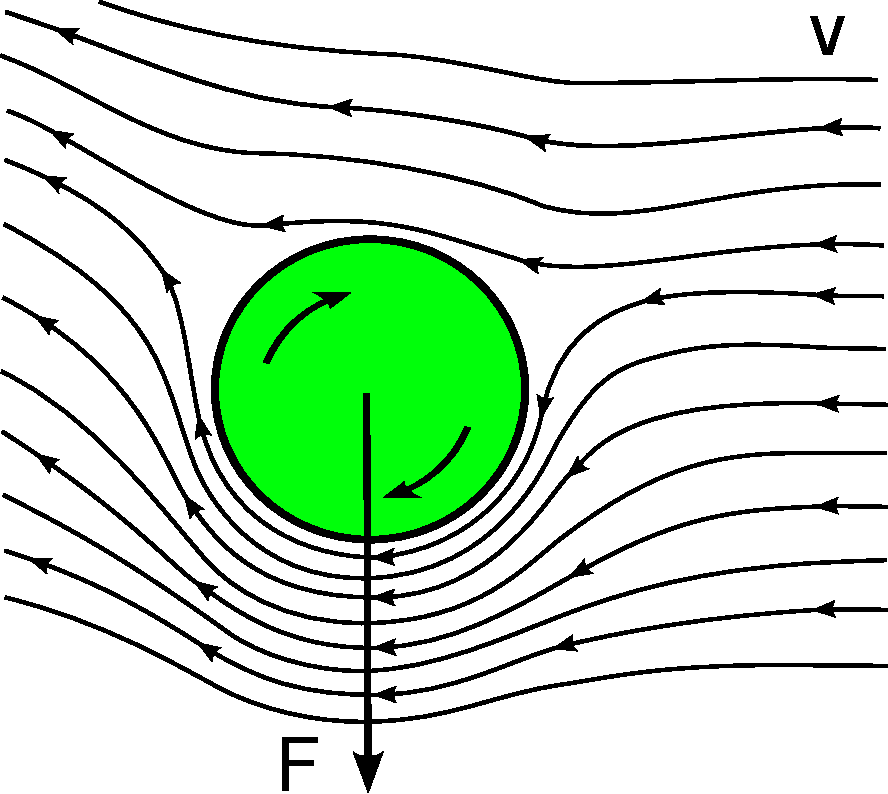
\includegraphics[width=5cm]{./Introduction_to_rocket_missile_tec/Magnus_effect.pdf}
\end{figure}
弹体绕自身对称轴旋转,使得两侧的的压强大小不一致,产生一个横向力$F$.

\section{火箭运动方程}
火箭在瞬时$t$的质量$M$和原质量$M_0$的关系时
\[
  M=M_0-\int_0^t \dot{m}\mathrm{d}t
\]
其中$\dot{m}$是质量变化率,为负值.
不考虑重力和气动力的情况下,火箭的速度称为理想速度,
是仅在发动机推力作用下火箭的速度.
于是
\[
  \mathrm{d}v=-u_e \frac{\mathrm{d}M }{M }
\]
也就是
\[
  v=-u_e \ln \frac{M}{M_0}
\]
记$\frac{M}{M_0}$为$\mu$,故火箭的理想末速度是
\begin{empheq}[box=\bluebox]{equation*}
  v_k=-u_e \ln \mu_k
\end{empheq}
\begin{note}
$\mu_k$是火箭的结构系数,是表示火箭结构设计优劣的一个
重要参数,用来衡量火箭的结构性能,$\mu_k$越小,火箭的速
度越大.
\end{note}
\begin{notice}
提高火箭的理想速度的两个方法:
\begin{enumerate}
  \item 提高燃气流的喷速$u_e$
  \item 降低火箭的结构系数$\mu_k$
\end{enumerate}
\end{notice}
\begin{example}
  现有一三级火箭,燃气的喷速均为$2200$m/s,结构
  系数均为$0.2$,求火箭的理想末速度.
  \[
    v=-3u_e \ln \mu_k=-3\times 2200\times \ln 0.2=10600\text{m/s}
  \]
\end{example}



%导弹的控制飞行原理
% % ! TEX root = ../mechanics.tex

\chapter{导弹的控制飞行原理}
导弹和普通武器的{\color{blue}本质区别}在
于导弹有制导系统.{\color{blue}制导系统}的基本任务
是确定导弹与目标的相对位置,操纵导弹飞行,
在一定的准确度下,引导导弹沿预定的弹道
飞向目标.

{\bfseries 控制力}\index{控制力}是控制
导弹质心运动的力.{\bfseries 操纵力}\index{操纵力}是
操纵导弹绕质心发生
转动的力.
\begin{notice}
	产生和改变控制力的方法:
	\begin{equation*}
		\color{titleblue}
		\begin{cases}
			 \text{有翼导弹:主要靠空气动力产生
			控制力}                     \\
			 \text{无翼导弹:主要靠发动机推力产生
				控制力}
		\end{cases}
	\end{equation*}
\end{notice}
用来产生操纵力矩的元件叫做{\color{blue}操纵元件}.
\begin{note}
	操纵元件除了产生操纵力矩对导弹起操纵作用
	外,它还可以对导弹起飞行稳定的作用.
\end{note}

\section{产生和改变控制力的方法}
\begin{equation*}
	\color{titleblue}
	\begin{cases}
		 利用空气动力来产生和改变控制力
		\begin{cases}
			轴对称导弹: & 有两对弹翼,在纵向对称平面           \\
			       & 和侧向对称平面内
			都能产生较             \\
			       & 大的空气动力.  \\
			面对面导弹: & 弹翼能产生
			较大的气动力,           \\
			       & 弹身和尾翼的空气
			动力较小.
		\end{cases}   \\
		 利用发动机推力来产生和改变控制力
	\end{cases}
\end{equation*}
\begin{note}
	这两种产生和改变控制力的方法的共同特点是:
	都需要依靠操纵元件使导弹绕质心转动.
\end{note}
\begin{notice}
	直接产生法向控制力的方法
	\begin{equation*}
		\color{titleblue}
		由火箭发动机直接产生法向控制力
		\begin{cases}
			 依靠旋转弯管型喷管直接产生法向
			控制力                \\
			 依靠侧向喷管直接产生法向控制力
		\end{cases}
	\end{equation*}
\end{notice}
\section{导弹的操纵元件}
\begin{equation*}
	\color{titleblue}
	\begin{cases}
		 空气动力舵面
		\begin{cases}
			 全动舵            \\
			 位于弹翼或尾翼后缘的舵和副翼 \\
			 翼尖舵和翼尖副舵       \\
			 转子副翼           \\
			 旋转弹翼           \\
			 扰流片
		\end{cases} \\
		 燃气动力操纵元件
		\begin{cases}
			 燃气舵               \\
			 摆动发动机             \\
			 摆动喷管              \\
			 摆帽(喷气流偏转器)        \\
			 燃气挡片              \\
			 向喷管内喷射气流或液体(二次喷射) \\
			 旋转弯管型喷管和侧喷管辅助发动机
		\end{cases}
	\end{cases}
\end{equation*}
\section{导弹制导原理}
 {\color{blue}制导系统}是完全操纵导弹飞向目标
任务所有设备的总和.
从准备发射到摧毁目标经过的三个阶
段:{\color{blue}发射控制,飞行控制,爆炸控制}.
\begin{note}
	控制系统的任务:操纵导弹执行引导系统发出的控制
	指令,控制导弹飞行目标.保证导弹在每一飞行段的
	稳定性.
\end{note}
\begin{align*}
	\color{titleblue}
	导弹的控制通道
	\begin{cases}
		 三通道控制
		\begin{cases}
			 俯仰 \\
			 偏航 \\
			 倾斜
		\end{cases} \\
		 双通道控制
		\begin{cases}
			 俯仰 \\
			 偏航
		\end{cases}
	\end{cases}
\end{align*}
\subsection{制导系统的分类}
\begin{equation*}
	\color{titleblue}
	制导系统
	\begin{cases}
		 自寻的系统
		\begin{cases}
			 主动式\text{:雷达,声学原理}         \\
			 半主动式\text{:雷达,激光}          \\
			 被动式\text{:雷达,红外,光学原理,声学原理}
		\end{cases} \\
		 遥控制导系统
		\begin{cases}
			 波束制导
       \begin{cases}
         无线电波束制导系统
         \text{:导弹自动沿雷达波束飞行}\\ 
         激光波束制导系统
         \text{:不易被干扰,精度高}
       \end{cases}\\
			 遥控指令制导\text{:目视,雷达,电视} \\
			 无线电制导                 \\
			 全球卫星制导
		\end{cases}      \\
		 自主制导
		\begin{cases}
			 惯性系统    \\
			 天文系统    \\
			 多普勒雷达系统 \\
			 地形匹配系统
		\end{cases}                  \\
		 复合制导系统
		\begin{cases}
			 自主+自动寻的系统    \\
			 自主+遥控系统      \\
			 遥控+自动寻的系统    \\
			 自主+遥控+自动寻的系统
		\end{cases}
	\end{cases}
\end{equation*}
\subsection{导弹的控制方式}
\begin{equation*}
	\color{titleblue}
	控制方式
	\begin{cases}
		 单通道控制,导弹自旋,一字舵面      \\
		 双通道控制,相互垂直的俯仰和偏航通道控制 \\
		 三通道控制,俯仰,偏航,倾斜三个通道控制
	\end{cases}
\end{equation*}
制导系统的基本要求如下
\begin{equation*}
	\color{titleblue}
	\begin{cases}
		 制导准确度(脱靶量)
		\begin{cases}
			 系统误差 \\
			 随机误差
		\end{cases}    \\
		 制导系统对目标的鉴别能力 \\
		 制导系统的可靠性     \\
		 制导系统的抗干扰能力
	\end{cases}
\end{equation*}
\begin{note}
	制导系统的制导误差主要取决于制导
	系统的动态误差,起伏误差,仪器误差.
\end{note}
\subsection{制导系统必须具备的功能}
\begin{enumerate}
	\item 导弹在飞行目标的过程中,要不断地
	      测量导弹的实际运动与理想运动之间的
	      偏差
	\item 根据偏差大小和方向形成控制指令,将
	      指令送到操纵元件,控制导弹改变运动状
	      态,消除该偏差
	\item 稳定导弹运动姿态角,使导弹始终保
	      持所需的姿态角
\end{enumerate}
\subsection{制导系统的组成}
{\bfseries 制导系统}是导引系统和控制系统的总称.
\begin{equation*}
	\color{titleblue}
	导引系统
	\begin{cases}
		测量装置 \text{:}& 测量目标和导弹的运动参数    \\
		程序装置  \text{:}&储存和发生使导弹按照预先规定
		的程序运动的参数和指令                    \\
		解算装置 \text{:}& 将测量装置测得的信息差经计算和
		变换后,形成控制指令信息输送给                \\
		     & 控制系统
	\end{cases}
\end{equation*}
\begin{equation*}
	\color{titleblue}
	控制系统
	\begin{cases}
		敏感装置 \text{:} & 感受和测量导弹的姿态角信息
		及重心运动信息                             \\
		综合装置  \text{:}& 将导引系统送来的信息与敏感装置
		送来的信息加以总和,                          \\
		      & 形成对导弹综合控制指令信息               \\
		放大变换器\text{:} & 将综合装置送来的指令信息进行
		校正,变换和功率放                           \\
		      & 大,使之称为推动执行机构工作的
		指令信息                                \\
		执行机构 \text{:} & 舵机与操纵元件组合的总称称为执行机构,
		它能根据指                               \\
		      & 令信息驱动操纵元件动作
	\end{cases}
\end{equation*}
\section{自主制导系统}
自主制导系统的基本原理
是:{\color{blue}按照发生前预先规定的程序或外界
固定的参考点作为基准来将导弹自动地导向目标}.
程序由导弹运动学参数与时间参数的一组固定关系组
成.固定的参考点可以利用卫星,星球,地理条件等.
\begin{note}
	自主自导系统的引导指令仅由弹上制导设备敏感
	地球或宇宙空间物质的物理特性产生,不与目
	标,制导站发生关联.
\end{note}
\subsection{测量,敏感装置}
\begin{equation*}
	\color{titleblue}
	\begin{cases}
		 陀螺仪
		\begin{cases}
			 定位陀螺仪,三个自由度,可测量
			两个方向的角偏移              \\
			 速率陀螺仪,两个自由度,可测量导弹
			绕某一坐标轴的角速度            \\
			 积分陀螺仪,可测量一个方向上的角偏移
		\end{cases} \\
		 飞行高度表
		\begin{cases}
			 气压式高度表,绝对高度 \\
			 无线电高度表,相对高度
		\end{cases}        \\
		 加速度计              \\
	\end{cases}
\end{equation*}
\begin{note}
	绝对高度是指到海平面的高度;相对高度是距
	地面的高度
\end{note}
陀螺仪的组成
\begin{equation*}
	\color{titleblue}
	\begin{cases}
		 转子,高速旋转,可绕轴转动    \\
		 内环架,通过轴和轴承固定在外环上 \\
		 外环架,通过轴和轴承固定在支架上
	\end{cases}
\end{equation*}
\begin{notice}
	陀螺仪的特性
	\begin{enumerate}
		\item {\bfseries 定轴性}:陀螺转子在惯性空间的
		      方位保持不变
		\item {\bfseries 进动性}:在主轴垂直的方向上
		      施加一外力矩$M$,则陀螺要绕着与外力
		      矩垂直的的方向转动
	\end{enumerate}
\end{notice}
干扰力矩的存在会引起转子轴缓慢的进动,
这个现象叫做陀螺
的 {\bfseries 漂移}\index{漂移}.
\begin{notice}
	使陀螺发生漂移的原因:
	\begin{enumerate}
		\item 轴承与传感器之间存在摩擦
		\item 陀螺仪本身制导的不对称和不平衡
	\end{enumerate}
\end{notice}
陀螺仪缓慢进动的角速度称为{\color{blue}漂移率或漂移
角速度}.
\begin{notice}
	减小漂移率的方法:
	\begin{enumerate}
		\item 增加转子的动量矩
		\item 减小干扰力
	\end{enumerate}
\end{notice}
\subsection{惯性制导系统}
{\color{blue}惯性制导}系统是利用导弹上的惯性
仪表来测量导弹的速度和坐标从而
形成指令信息来导引导弹的系统.
\begin{equation*}
  \color{titleblue}
  惯性制导系统
  \begin{cases}
    平台制导系统,将加速度计安装在
    陀螺稳定平台上\\ 
    捷联制导系统,将加速度计与导弹固连
  \end{cases}
\end{equation*}
\begin{notice}
  捷联制导系统的优缺点:
  \begin{enumerate}
    \item 优点:\\ 
      简化了系统,可靠性高
    \item 缺点:\\ 
      由于加速度计与导弹固连而
      处于相当苛刻的振动环境中,
      影响制导精度
  \end{enumerate}
\end{notice}
惯性制导系统
{\color{blue}完全自动地控制导弹飞行,具有
优秀的抗干扰能力}.但是,该系统中陀螺仪
{\color{blue}存在
漂移误差,该误差会积累}.

\subsection{天文制导系统}
利用测量恒星的方法来确定导弹的位置,一般
测量两颗恒星的位置.

天文制导系统完全自动化,不受外界的干扰.

\subsection{多普勒雷达制导系统}
多普勒制导系统往往用于复合制导系统中,用
来校正其他系统的误差.

\subsection{地形匹配系统}
利用某已知地区的地形特征作为标志,根据导弹
当下弹道测量的地形特征和预定弹道下的地形
特征做比较,来校正导弹的弹道,使导弹按照预定
路线导向目标.
\begin{note}
不能用于没有地形差别的海平面和平原地区.
\end{note}
\section{遥控制导系统}
{\color{blue}遥控制导系统}是由导弹以外的制导站
向导弹发送引导信息的制导系统.
\begin{equation*}
  \color{titleblue}
  遥控制导系统
  \begin{cases}
    指令制导系统
    \begin{cases}
      有线指令系统\\ 
      无线电指令系统
      \begin{cases}
        目视\\ 
        雷达自动跟踪
      \end{cases}\\ 
      电视指令系统
      \begin{cases}
        优点\text{:导引精度高}\\ 
        缺点\text{:容易受敌方干扰和天气影响}
      \end{cases}
    \end{cases}\\ 
    波束制导系统\\ 
    无线电导航制导系统
  \end{cases}
\end{equation*}

\begin{notice}
遥控制导系统的优缺点:
\begin{enumerate}
  \item 优点:\\ 
    制导精度高,制导距离比自寻的系统稍远,弹
    上制导设备简单
  \item 缺点:\\ 
  制导精度随导弹离制导站的距离增大而
    减小,且易受外界干扰
\end{enumerate}
\end{notice}
多用于地空,空空,空地导弹.

指令制导系统的组成
\begin{equation*}
  \color{titleblue}
  指令制导系统
  \begin{cases}
    观测装置\\ 
    指令形成装置\\ 
    控制线
  \end{cases}
\end{equation*}

电视导引系统的分类
\begin{equation*}
  \color{titleblue}
  \begin{cases}
    自动寻式的电视制导系统\\ 
    遥控式的电视指令制导系统
  \end{cases}
\end{equation*}
\section{自动寻的制导系统}
{\color{blue}自动寻的制导系统}是
目标辐射或反射的能量导引导弹去攻击
目标.
\begin{note}
自动寻的制导系统要求背景有足够的
能量对比性
\end{note}
\begin{notice}
自动寻的制导系统的三种类型:
\begin{enumerate}
  \item 主动式:\\ 
    照射目标的能源在导弹上,并且导弹接受
    目标反射回来的能量
  \item 半主动式:\\ 
    照射目标的能源在地面制导站或者其他位
    置,导弹上只有接收装置,制导距离比主动式
    大
  \item 被动式:\\ 
    目标本身就是辐射能源,不需要发射装置,弹上
    只有接受装置,导引头接受辐射能量
\end{enumerate}
\end{notice}
雷达自动寻的制导系统分类
\begin{equation*}
  \color{titleblue}
  \begin{cases}
    半主动式\text{:接收装置在导弹上}\\ 
    主动式\text{:发射和接收装置都在导弹上}
  \end{cases}
\end{equation*}
\begin{note}
缺点是容易受干扰
\end{note}
红外自动寻的制导系统分类
\begin{equation*}
  \color{titleblue}
  \begin{cases}
    半主动式\text{:接收装置在导弹上}\\ 
    主动式\text{:发射和接收装置都在导弹上}
  \end{cases}
\end{equation*}
\begin{equation*}
  \color{titleblue}
  \begin{cases}
    红外点源\text{:将目标看成是一个点}\\ 
    红外成像制导系统\text{:将目标的形状用红外绘制出来}
  \end{cases}
\end{equation*}
\begin{note}
红外导引头由红外探测系统和电子线路两部分组成.
\end{note}

激光自动寻的制导系统接收的是来自
激光发射器照射目标的反射激光,多用于半
主动式自动寻的制导系统中.

电视自动寻的制导系统的主要部件是
一部电视摄像机.
\begin{note}
电视自寻的制导系统具有被动式自动寻的制导
系统的优点,抗干扰性较强,隐蔽性好.
\end{note}
\section{舵机}
导弹控制系统的{\color{blue}执行机构}是根据控制指令信息来
驱动舵机带动操纵元件使弹体作出相应的姿态变
化.
\begin{equation*}
  \color{titleblue}
  舵机
  \begin{cases}
    气压式
    \begin{cases}
      冷气式舵机\text{:能源是贮存在容器中的
      压缩气体}\\ 
      燃气式舵机\text{:以燃气作为能源}\\ 
    \end{cases}\\ 
    液压式\text{:用一定压力的液压油作为舵机的能源}\\ 
    电磁式\\ 
    电动式\text{:主要是一台电机和减速装置}
  \end{cases}
\end{equation*}
\begin{notice}
几种舵机的优缺点
\begin{enumerate}
  \item 气压式舵机: 
  \begin{enumerate}
    \item 优点:\\ 
      简单,工作可靠
    \item 缺点:\\ 
      延时较大,快速性较差
  \end{enumerate}
\item 液压式舵机:
  \begin{enumerate}
    \item 优点:\\ 
      延时小,功率大,响应速度快
    \item 缺点:\\ 
      比其他舵机结构复杂,成本高
  \end{enumerate}
\item 电磁式舵机: 
  \begin{enumerate}
    \item 优点:\\ 
      结构简单,重量轻,需要的能量
      小,可靠性高
    \item 缺点:\\ 
      输出功率小
  \end{enumerate}
\end{enumerate}
\end{notice}


%火箭,导弹的飞行力学
% % ! TEX root = ../mechanics.tex
\chapter{火箭导弹的飞行力学}
作用在火箭弹的力有{\color{blue}发动机
推力$P$,火箭弹重力$G$,总空气动力$R$.}作
用在火箭弹上主要力矩有{\color{blue}俯仰力
矩$M_\theta$,偏航力矩$M_\Phi$,滚转
力矩$M_\gamma$}.
\begin{note}
	总空气动力作用在压心上,同时产生空气力矩.
\end{note}
火箭弹的运动方程中共有$9$个参数,即
速度$v$,弹道倾角$\theta$,攻角$\alpha$,俯仰
角$\Phi$,弹道坐标参数$x$,$y$和时间$t$,共有
$8$个方程,除时间$t$外,其余参数都可以看成是
时间$t$的函数.
\section{火箭弹的弹道}
\subsection{弹道特性}
火箭弹的弹道具有两个连续的区段,即
{\color{blue}主动段和被动段}.

若火箭弹在真空中飞行,无空气动力作用,射程
$x$则为
\[
	x=\frac{v_0^2 \sin 2\theta_0}{g }
\]
\begin{note}
	射程仅仅取决于主动段终点的速度$v_0$和
	弹道倾角$\theta_0$
\end{note}
\section{密集度问题}
设计精度用对目标的命中概率描述,包含
{\color{blue}准确度和密集度}两部分.
{\bfseries 准确度}\index{准确度}是
指火箭弹炸点散布中心偏离射击指向点的程度.
{\bfseries 密集度}\index{密集度}是
各火箭弹炸点围绕散布中心的密集程度.
\begin{note}
	密集度高不代表准确度好;准确度好不代表
	密集度高
\end{note}
引起导弹散布的误差根源:
\begin{equation*}
	\color{red}
	\begin{cases}
		方向密集度
		\begin{cases}
			横风的不一致和扰动气流 \\
			火箭弹离轨时的初始扰动 \\
			推力偏心和空气动力偏心 \\
			质量偏心和动不平衡
		\end{cases} \\
		距离密集度
		\begin{cases}
			火药装药质量不一致        \\
			火药装药比冲量不一致       \\
			火箭弹弹体质量不一致       \\
			火箭弹弹体加工公差引起的比冲量变化 \\
			飞行过程中阻力变化
		\end{cases}
	\end{cases}
\end{equation*}
\section{导弹的飞行弹道}
制导弹道按形成的特点可以分为:
\begin{equation*}
	\color{titleblue}
	\begin{cases}
		用于攻击固定目标的\text{:}整个
		弹道或大部分弹道在发射前就被制导
		系统预先确定 \\
		用于攻击活动目标的\text{:}弹道
		在发射前不能预先确定,是一种随机弹道
	\end{cases}
\end{equation*}
\begin{notice}
	弹道式导弹和无控火箭弹弹道的区别是:
	\begin{enumerate}
		\item 主动段有控制力和控制力矩
		\item 被动段不是抛物线形式,而是
		      椭圆曲线形弹道
	\end{enumerate}
\end{notice}
\subsection{弹道式导弹弹道的分段}
\begin{equation*}
	\color{titleblue}
	\begin{cases}
		主动段
		\begin{cases}
			垂直上升段  \\
			转弯飞行段  \\
			发动机关车段 \\
		\end{cases} \\
		被动段
		\begin{cases}
			自由飞行段 \\
			再入段
		\end{cases}
	\end{cases}
\end{equation*}
\begin{note}
	弹道式导弹只在主动段上制导
\end{note}
\section{有翼式导弹的弹道}
有翼式导弹的飞行路线是根据某种
与目标的相对关系来控制的.

导弹和目标之间的相对运动所
遵循的规律称为{\color{blue}导引规律},此时
的弹道称为{\color{blue}导引弹道}.

导弹与目标的连线称为
{\bfseries 目标线}\index{目标线}.

导弹速度矢量与目标线的夹角称为
{\bfseries 导弹前置角}\index{导弹前置角}.

飞行弹道可分为
\begin{equation*}
	\color{titleblue}
	\begin{cases}
		追踪导引弹道\text{:}导弹的速度矢量
		始终指向目标         \\
		平行接近法的飞行弹道\text{:}导引过程
		中目标线在空间的位置始终不变 \\
		三点法的飞行弹道\text{:}导弹,目标,制导站
		始终连成一线
	\end{cases}
\end{equation*}
\begin{notice}
	几种弹道的优缺点:
	\begin{enumerate}
		\item 追踪导引弹道:
		      \begin{enumerate}
			      \item 优点:\\
			            简单
			      \item 缺点:\\
			            当导弹需要迎面射击目标时,或追踪
			            近距离高速目标时,可能会出现弯曲度
			            过大的弹道,导弹要承受过大的载荷
		      \end{enumerate}
		\item 平行接近法弹道:
		      \begin{enumerate}
			      \item 优点:\\
			            当导弹迎向目标或近距离高速飞行目标时
			            ,弹道弯曲程度小,法向过载要求小
			      \item 缺点:\\
			            制导系统复杂,实现困难
		      \end{enumerate}
		\item 三点法的飞行弹道:
		      \begin{enumerate}
			      \item 优点:\\
			            制导简单,抗电子干扰能力强
			      \item 缺点:\\ 
              当导弹迎着目标或近距离高速飞行目标时,
              弹道弯曲程度大,法向过载要求大
		      \end{enumerate}
	\end{enumerate}
\end{notice}
\section{导弹的机动性,过载,稳定性及操纵性}
{\bfseries 机动性}\index{机动性}:指导弹能
迅速改变飞行速度的大小和方向的能力.
\begin{note}
可用导弹在飞行过程中所能产生的切向加速度和
法向加速度的大小来评定导弹机动性的好坏
\end{note}

对于有翼导弹,法向机动性取决于法向空气动力的
大小;对于采用推力控制飞行的导弹,法向机动性
取决于发动机推力的大小及其可能偏向弹体轴线
角度的大小.

\begin{notice}
影响导弹机动性的因素
\begin{enumerate}
  \item 导弹的气动特性
  \item 导弹的质量大小
  \item 弹道倾角$\theta$的大小
  \item 飞行的高度.高度越高大气密度越低,
    法向机动性就要下降.
  \item 弹翼的面积.弹翼面积越大,法向机动性
    就越好.
\end{enumerate}
\end{notice}

{\bfseries 过载}\index{过载}指作用在导弹
上外力的大小和导弹重量的比值.
\[
  n=\frac{N}{G }
\]
\begin{note}
过载是一个向量,方向与外力$\mathbf{N}$的
方向一致.是一个无量纲的量.
\end{note}
\begin{notice}
限制导弹过载的因素:
\begin{enumerate}
  \item 导弹操纵元件的偏转范围是有限的
  \item 产生气动法向力的攻角和侧滑角不可能
    太大,不能超过它们的临界值
  \item 导弹弹体的结构不允许法向力很大,否则
    弹体将遭到破坏
\end{enumerate}
\end{notice}

{\bfseries 稳定性}\index{稳定性}指导弹在飞行
过载中,由于受到某种干扰,使其偏离原来的飞行状
态,当干扰消失后,导弹恢复原来飞行状态的能力.
\begin{note}
只要保证气动力的焦点位于质心之后,并且有一段距离,
就可以保证攻角$\alpha$是稳定的,如果弹上装有自稳定
系统,则无此要求
\end{note}

{\bfseries 操纵性}\index{操纵性}指导弹在操纵元件
发生动作时,改变其原来飞行状态的能力以及对此
反应快慢的程度.
\begin{note}
导弹的稳定性和操纵性时对立统一的
\end{note}
\begin{notice}
稳定性和操纵性的对立统一:
\begin{enumerate}
  \item 对立性:\\ 
    导弹的操纵性越好,导弹就越容易改变其原来的
    飞行状态;导弹的操纵性越差,导弹就越难改变
    其原来的飞行状态.因此,提高导弹的操纵性,就
    会削弱导弹的稳定性,反之亦然.
  \item 统一性:\\ 
    静稳定性差或者静不稳定的导弹,则要求自动稳定
    系统使操纵元件发生动作从而产生操纵力矩,以便
    对导弹进行操纵,来克服外加干扰维持导弹的稳定.
    在这种情况下,如果导弹的操纵性好,导弹在自动
    稳定系统的作用下,能够较快地改变其飞行状态,
    使导弹快速达到稳定.因此,导弹的操纵性有助于
    加强导弹的稳定性.
\end{enumerate}
\end{notice}



%导弹的气动布局
% % ! TEX root = ../mechanics.tex
\chapter{导弹的气动布局}
\section{火箭弹稳定装置的基本类型}
\begin{equation*}
  \color{titleblue}
  两种尾翼
  \begin{cases}
    弧形张开式尾翼
    \begin{cases}
      整流罩\\ 
      弧形翼片\\ 
      连接轴\\ 
      同步环
    \end{cases}\\ 
    刀形张开式尾翼
    \begin{cases}
      尾翼座\\ 
      刀形翼片
      \begin{cases}
            前张式\\ 
            后张式
          \end{cases}\\ 
      翼片转轴
    \end{cases}
  \end{cases}
\end{equation*}
\begin{equation*}
  \color{titleblue}
  尾翼的分类
  \begin{cases}
    按尾翼刚度分
    \begin{cases}
      刚性尾翼\\ 
      弹性尾翼
    \end{cases}\\ 
    按尾翼尺寸和弹径关系分
    \begin{cases}
      同口径尾翼\\ 
      超口径尾翼
    \end{cases}\\ 
    按翼片和弹体的联接方式分
    \begin{cases}
      固定式尾翼\\ 
      张开式尾翼
    \end{cases}\\ 
    按尾翼平面形状分
    \begin{cases}
      矩形尾翼\\ 
      梯形尾翼\\ 
      三角形尾翼\\ 
      刀形尾翼
    \end{cases}
  \end{cases}
\end{equation*}
\begin{notice}
两种尾翼的特点
\begin{enumerate}
  \item 弧形张开式尾翼
    \begin{enumerate}
      \item 平时合拢在弹体上,最大外径不超过
        弹体直径,结构紧凑.
      \item 四片尾翼同时张开
      \item 翼片弧长最大不能超过弹体的$\frac{1}{4}$
        周长,为提供足够升力必须加大弦向尺寸.
      \item 翼片根部容易出现强度不足的问题.
    \end{enumerate}
  \item 刀形张开式尾翼
    \begin{enumerate}
      \item 翼片张开动力可选弹簧力,弹体自旋离心力等
      \item 能充分利用弹上的空间.
      \item 展向尺寸较大,为提高强度需加厚,阻力较大.
    \end{enumerate}
\end{enumerate}
\end{notice}

\subsection{尾翼的几何参数}
{\bfseries 展长}\index{展长}指机翼左右翼尖之间的距离.

{\bfseries 弦长}\index{弦长}指机翼前缘到机翼后缘之间的
距离.

{\bfseries 后掠角}\index{后掠角}指机翼设计中心线和机身
之间的夹角.

尾翼的主要参数包括{\color{blue}展弦比$\lambda$,后
掠角$\chi$,根稍比$\eta$,相对厚度$\overline{c}$,翼片
数$N$以及剖面形状}.

\begin{notice}
翼面参数的影响
\begin{enumerate}
  \item 展弦比:\\ 
    对亚音速飞行的火箭弹,增大展弦比可以减小阻力;当
    火箭弹超音速飞行时,增大展弦比会增大阻力.
  \item 后掠角:\\ 
    后掠角的作用时提高翼面的临界马赫数,以延缓前缘波
    阻的产生,从而有效的降低尾翼阻力系数的值.后掠角
    越大,临界马赫数就越大,火箭弹在低超音速飞行时,
    激波出现的可能性就越小,从而阻力减小.
  \item 根稍比:\\ 
    根稍比对气动力影响不显著.根稍比大的尾翼,气动载荷
    分布更靠近根部.梯形尾翼和三角翼气动性能差异小,但
    梯形尾翼翼尖刚度高.
  \item 相对厚度:\\ 
    尾翼的相对厚度主要影响阻力.厚度增加,阻力总是增加的.
    在保证强度,刚度条件下,应尽可能减小相对厚度.
  \item 剖面形状:\\ 
    剖面形状主要影响厚度波阻.选择翼剖面形状时,既要
    考虑尾翼的气动特性,又要考虑强度,刚度及加工工艺
    特性.
  \item 翼片数量:\\ 
    尾翼段阻力系数与翼片对数成正比,而增加$N$时,升力
    系数增加较小.
\end{enumerate}
\end{notice}
{\color{blue}
\begin{itemize}
  \item 减小展弦比,增加根稍比,可以使尾翼结构质量降低.
  \item 减小相对厚度,对实心结构的翼剖面来说,可以使
    尾翼的质量降低.
\end{itemize}}
在设计尾翼时,满足结构设计和飞行稳定性的条件下,应采用
小展弦比,大根稍比,小相对厚度.
\section{导弹的气动外形}
有翼导弹的升力,控制力主要由弹身,翼面,舵面产生.

  翼面沿周向的配置如下图
\begin{figure}[!ht]
  \centering 
  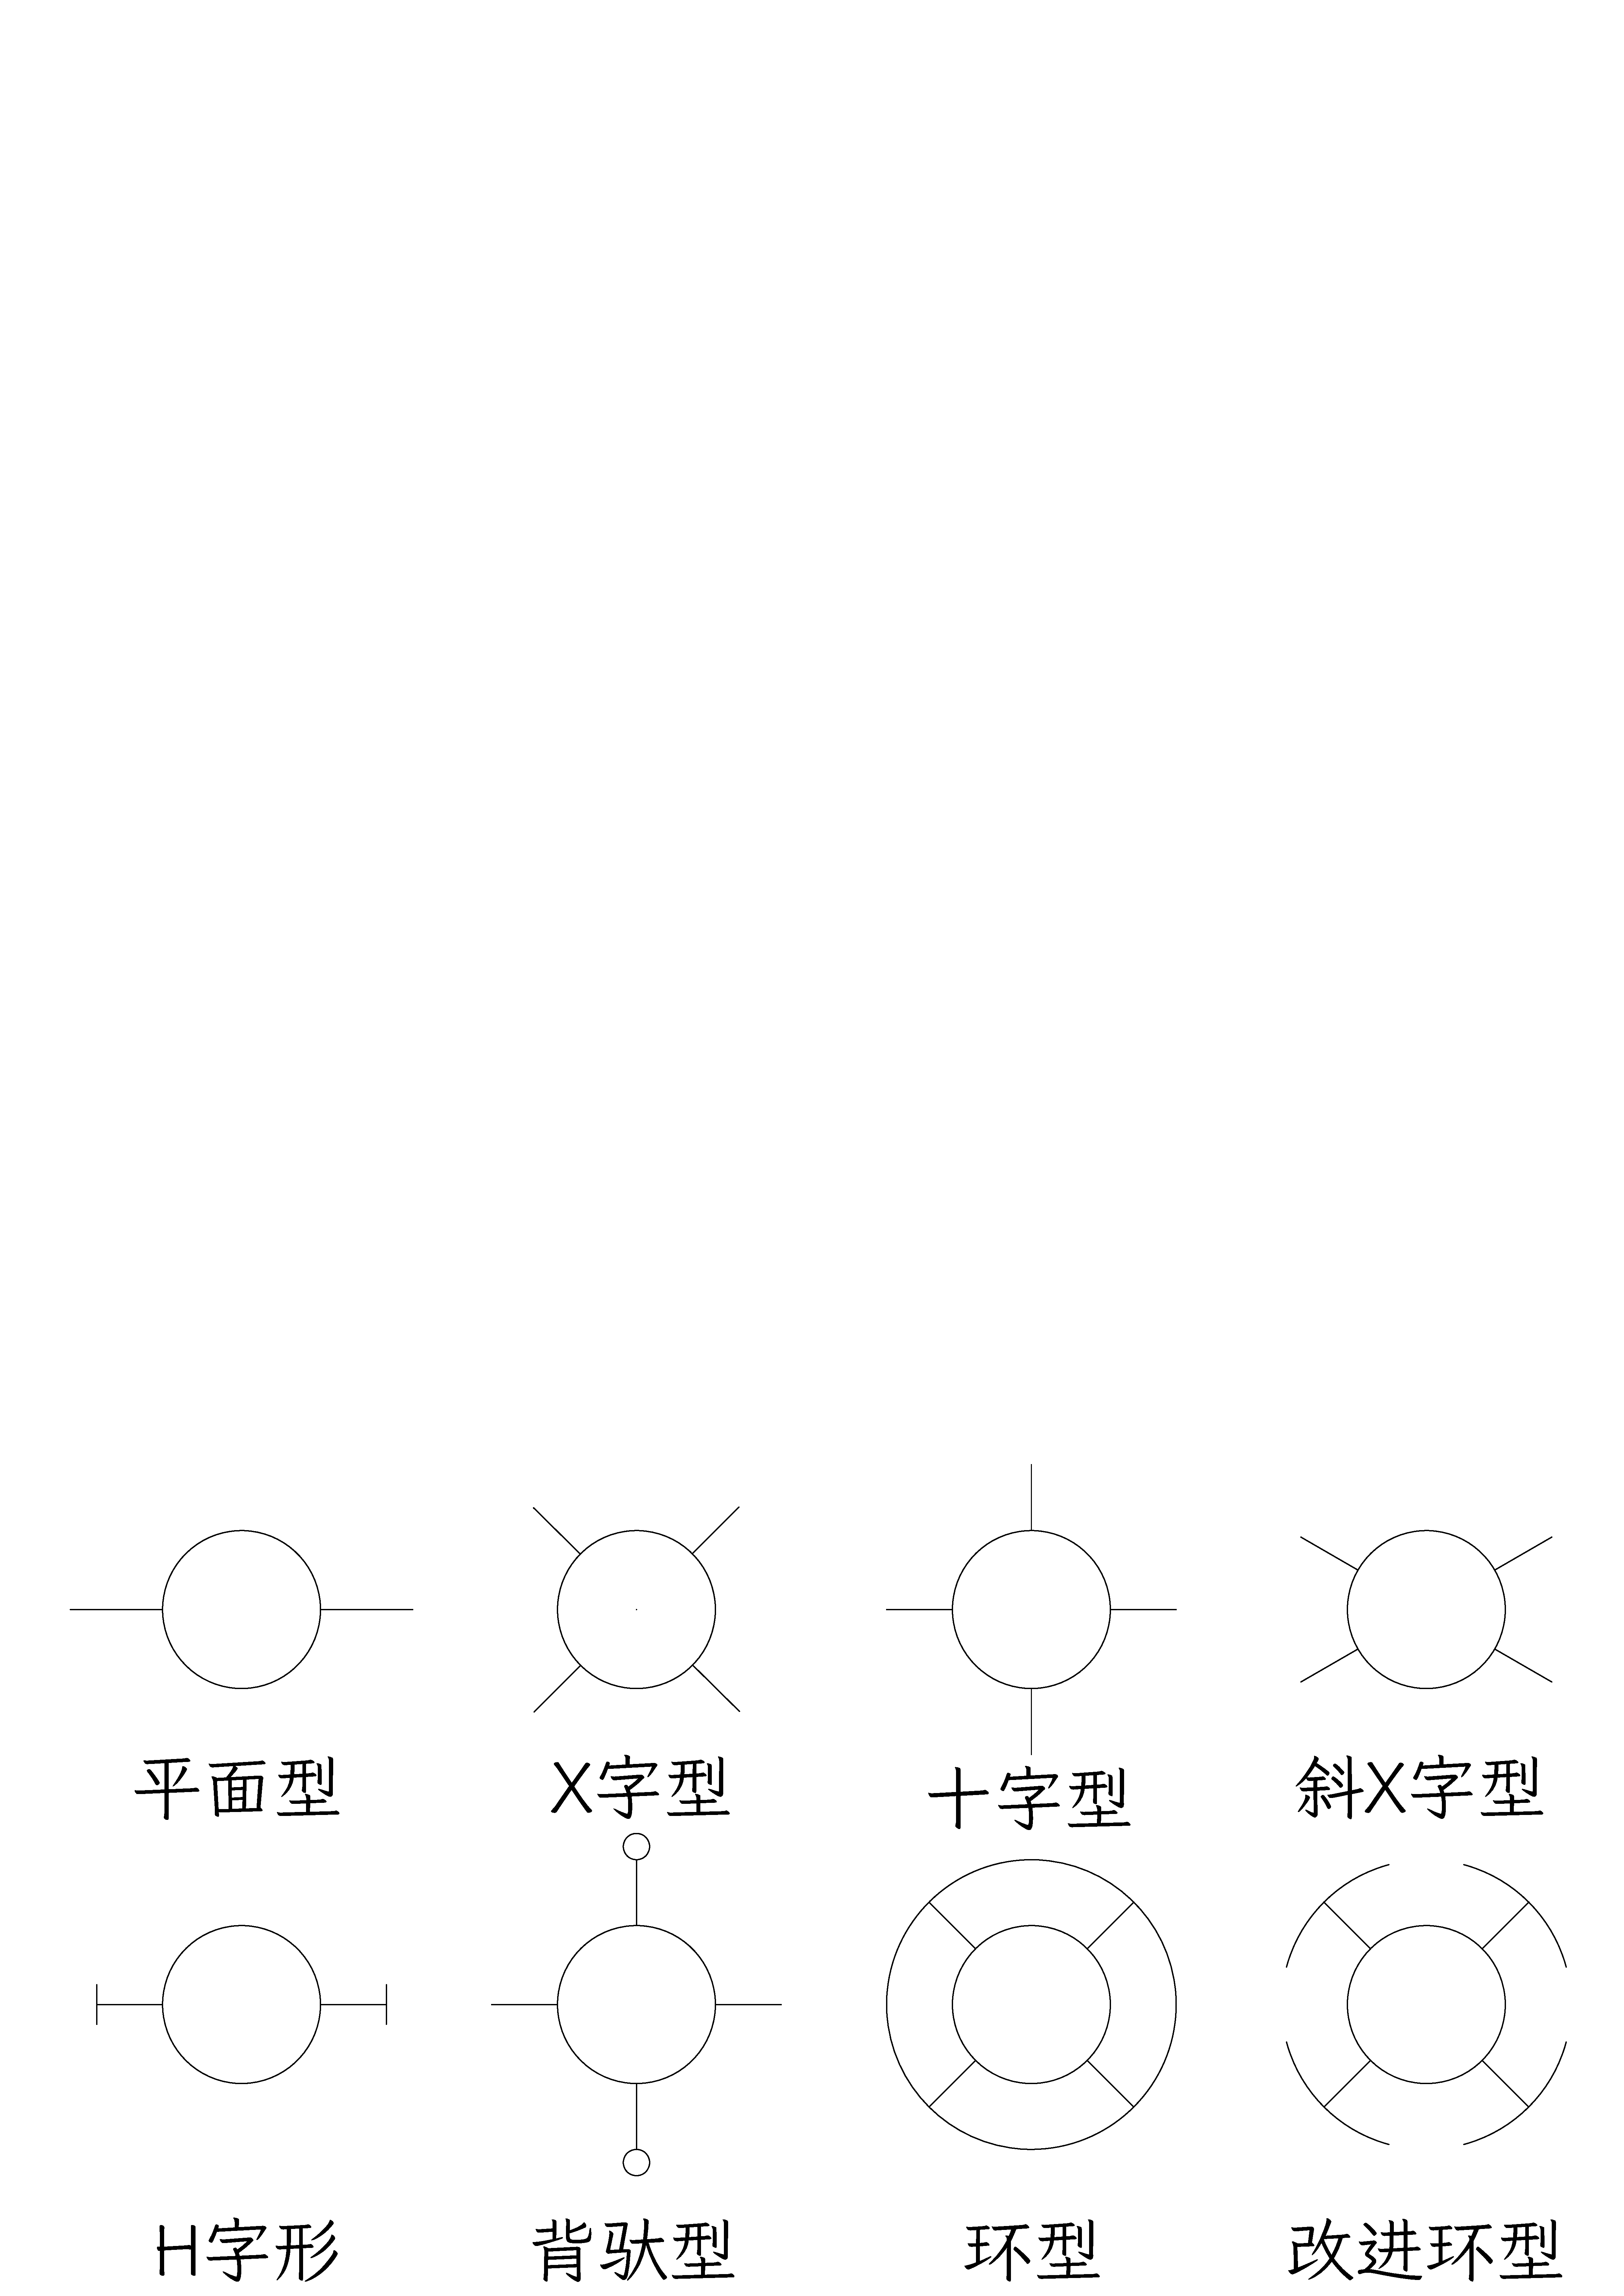
\includegraphics[width=9cm]{./Introduction_to_rocket_missile_tec/wings.pdf}
\end{figure}

\begin{equation*}
  \color{titleblue}
  翼面沿弹身轴向的布局
  \begin{cases}
    正常式\text{:}弹翼在前,操纵面在后\\ 
    鸭式\text{:}弹翼在后,操纵面在前\\ 
    旋转弹翼式\text{:}弹翼在前,同时又是
    操纵面:固定尾翼在后,起稳定作用\\ 
    无尾式\text{:}操纵面位于弹翼的后缘\\ 
    无弹翼式\text{:}尾部是操纵面,升力依靠
    弹身产生
  \end{cases}
\end{equation*}
\begin{notice}
翼面沿弹身纵向配置型式与控制特点:
\begin{enumerate}
  \item 正常式布局:\\ 
    正常式布局弹翼配置在弹身中段,舵面处于弹身
    尾段,且两组翼面通常为X-X型配置.

    条形翼可以利用翼体干扰提升升力,减质减阻.
    压心变化小,翼展小.

    特点是:
    \begin{enumerate}
      \item 由于舵面负偏转角产生一个使头部上抬的力矩
        ,所以舵面偏转角和弹体攻角相反.舵面产生的控制力
        的方向也始终与弹体攻角产生的升力方向相反,导弹的
        响应特性比较差.
      \item 升力特性和响应特性较鸭式布局和全动翼要差.
      \item 弹翼固定不偏转,空气动力的线性程度较其他两种
        布局要好些.
    \end{enumerate}
  \item 无翼式布局:\\ 
    实际就是全动翼式,整个弹翼做成可转动的.既可起翼的作用,
    又可以起舵的作用.可以提供很大的法向力(大机动过载).
    
    特点是:
    \begin{enumerate}
      \item 具有需要的过载特性
      \item 大大改善了非对称气动力特性
      \item 具有较高的舵面效率和需要的纵向静稳定性
      \item 具有较轻的质量和较小的气动阻力
      \item 结构简单,操作方便,使用性能好
    \end{enumerate}
  \item 鸭式布局:\\ 
    翼面布局与正常式相反,小的舵面位于弹身前部,大的弹翼
    位于弹身中后部.
    
    特点是:
    \begin{enumerate}
      \item 鸭式舵偏转方向始终与攻角一致,故其升阻比大
      \item 舵直接提供升力,反应快
      \item 舵在前部,舵面效率高
      \item 舵面与安定翼远离质心,便于静稳定度的调整
      \item 舵面展小,面积小,对后翼面下洗流影响小
      \item 舵面产生的升力近乎被安定翼由于舵面下洗
        而减小的升力相抵消,全弹的升力与舵面升力无关
      \item 鸭式舵{\color{red}很难作滚动控制}
    \end{enumerate}
    很难作滚动控制的解决方法是:
    \begin{enumerate}
      \item 减小尾翼翼展,以减小反滚转力矩
      \item 采用环形尾翼
      \item 采用新型的自由旋转尾翼
      \item 环形翼的基础上,采用T型翼片组合尾翼的布局
      \item 近距离耦合式鸭式布局(P119页)
      \item 断牙形前缘鸭式舵布局(P119页)
    \end{enumerate}
  \item 旋转弹翼布局:\\ 
    弹翼旋转,起控制舵的作用.尾翼固定,起稳定翼的作用.
    法向力主要靠旋转翼提供,升力靠弹翼偏转直接产生.
    质心位于升力作用点后,质心位置最有利.
  \item 无尾式布局:\\ 
    见P122页
\end{enumerate}
\end{notice}

导弹总体设计的核心是{\color{blue}外形设计和
气动力设计}.

导弹外形设计的两个任务:
\begin{enumerate}
  \item 导弹各部件的几何参数选择及几何尺寸的计算与确定
  \item 对弹上各部件进行气动布局,合力确定各部件的位置
    与布局形式
\end{enumerate}

气动布局的要求:
\begin{enumerate}
  \item 满足导弹战术技术指标和弹上各系统工作
    要求
  \item 充分利用最佳翼身干扰和翼面间干扰以及
    外挂物与翼身的干扰,设计出最优升阻比的外形
    配置
  \item 在作战空域内,导弹要满足机动性,稳定性
    和操纵性的要求
  \item 保证在最大使用攻角范围内,空气动力学
    特性尽可能处于线性范围,尤其是力矩特性
  \item 气动控制面设计要保证在使用攻角和速度
    范围内,压心变化尽可能小
  \item 便于运输,贮存和实战使用
\end{enumerate}


%火箭导弹的动力装置
% % ! TEX root = ../mechanics.tex
\chapter{火箭导弹的动力装置}
\begin{equation*}
	\color{titleblue}
	发动机
	\begin{cases}
		火箭发动机
		\begin{cases}
			固体火箭发动机 \\
			液体火箭发动机
		\end{cases} \\
		空气喷气发动机
		\begin{cases}
			涡轮喷气发动机  \\
			涡轮风扇发动机  \\
			涡轮螺旋桨发动机 \\
			冲压发动机
		\end{cases}
	\end{cases}
\end{equation*}
{\color{blue}火箭动力装置}是为火箭飞行提供动力
的装置,推进系统保证火箭获得所需的
作战射程和飞行速度等特性.

发动机总体技术要求和依据如下:
\begin{enumerate}
	\item 功能和要求
	\item 发动机的总冲量,比冲量,推力
	      时间曲线
	\item 对发动机燃气流的特殊要求:无烟,少烟等
	\item 质量,尺寸要求
	\item 布局设计及结构对接要求
	\item 可靠性及寿命周期
	\item 安全性
	\item 启动特性
	\item 经济性
\end{enumerate}

选择发动机的一般原则
\begin{enumerate}
	\item 工作时间
	\item 对全弹质量的影响:发动机本身的质量,
	      迎面阻力,燃料消耗量
	\item 性能影响
	\item 对发动机的掌握程度
\end{enumerate}
选择方法
\begin{enumerate}
	\item 比冲与马赫数的关系
	\item 耗油量与马赫数的关系
	\item 推力质量比与马赫数的关系
	\item 推力最大迎风面积比与马赫数的关系
\end{enumerate}

火箭发动机的主要性能参数
\begin{equation*}
	\color{titleblue}
	\begin{cases}
		总冲量    \\
		推力     \\
		工作时间   \\
		火箭发动机的高度特性,空气喷气发动速度和
		高度特性   \\
		比冲     \\
		推力质量比  \\
		质量比    \\
		单位迎面推力 \\
		推力曲线设计及实现
	\end{cases}
\end{equation*}

{\bfseries 比冲}\index{比冲}:发动机消耗单位推进剂质量
产生的冲量.

{\bfseries 推力质量比}\index{推力质量比}:发动机的推力
与动力装置结构的净质量(不含燃料)的比值.

{\bfseries 质量比}\index{质量比}:推进剂质量与动力
装置总质量的比值.

{\bfseries 单位迎面推力}\index{单位迎面推力}:发动机
推力与其最大横截面积的比值.

\section{固体火箭发动机}
结构:{\color{blue}推进剂,燃烧室,喷管和点火装置}.

固体火箭发动机的特点:
\begin{itemize}
	\item 结构简单
	\item 可在短时间内产生大推力
	\item 使用简单,工作可靠,可长期贮存
	\item 机动性好
\end{itemize}

工作原理,主要分为两个过程:
\begin{enumerate}
	\item 装药在燃烧室里面燃烧的过程.装药
	      的大部分化学能释放出来,转变为燃烧产物的
	      热能和压力能
	\item 燃气在喷管中的膨胀过程.燃气随着压力
	      和温度的下降而膨胀,压力能和热能转变为
	      动能
\end{enumerate}

固体推进剂的分类:
\begin{equation*}
	\color{titleblue}
	\begin{cases}
		均质火药
		\begin{cases}
			单质药,硝化纤维为主 \\
			双基药
			\begin{cases}
				硝化纤维 \\
				硝化甘油
			\end{cases}
		\end{cases} \\
		异质火药
		\begin{cases}
			复合药
			\begin{cases}
				氧化剂 \\
				燃烧粘结剂
			\end{cases} \\
			黑火药
		\end{cases}
	\end{cases}
\end{equation*}

改进型双基药:双基药中加入过氯酸铵,铝粉或黑索金等.

对固体推进剂的要求
\begin{itemize}
	\item 能量性能,能量大,比重大
	\item 燃烧性能,燃烧时稳定性好
	\item 机械性能,贮存,运输时不会发生断裂
	\item 安定性能,具有良好的物理安定性和化学
	      安定性
	\item 生产经济性能
\end{itemize}

药柱截面的几何形状和燃烧表面积随时间的
变化规律决定了发动机推力随时间变化的
规律.

固体火箭发动机的分类
\begin{equation*}
  \color{titleblue}
  \begin{cases}
    自由装填式
    \begin{cases}
      发动机顶盖,头部支撑弹性件\\ 
      点火装置\\ 
      药柱,药柱包覆层,挡药板\\ 
      燃烧室壳体\\ 
      隔热层\\ 
      喷管
    \end{cases}\\ 
    浇注式
    \begin{cases}
      顶盖,底盖,堵盖\\ 
      点火装置\\ 
      燃烧室壳体\\ 
      石墨衬套\\ 
      药柱\\ 
      喷管
    \end{cases}
  \end{cases}
\end{equation*}

对于固体火箭发动机,采用石墨喉衬解决耐热问题.

\section{液体火箭发动机}
结构:{\color{blue}燃烧室,推进剂贮箱,输送系统}.

液体火箭发动机的燃料分类
\begin{enumerate}
	\item 单组元:\\
	      含燃烧机和氧化剂,特点是常温常压稳定,
	      加热,加压或接触触媒剂时分解.输送系统简单.
	      用于副系统中或涡轮泵组能源.
	\item 双组元:\\
	      燃烧剂和氧化剂在喷入燃烧室前不混合.
	\item 三组元:\\
	      液氧/烃+液氧三组元
\end{enumerate}

对液体推进剂的要求:
\begin{itemize}
	\item 高比冲
	\item 无腐蚀,无毒,物理性能稳定,冰点低,比重大,物理性能稳定
	\item 一种组元比热大,化学稳定性好,流量大,可用来冷却
	\item 粘度小
	\item 燃烧速度快,点火时间短,不发生有害的振荡
\end{itemize}

液体火箭发动机的组成
\begin{equation*}
	\color{titleblue}
	\begin{cases}
		推进剂输送系统  \\
		流量调节控制活门 \\
		冷却系统     \\
		推力室      \\
		固定零部件
	\end{cases}
\end{equation*}

推进剂输送系统的分类:
\begin{equation*}
	\color{titleblue}
	\begin{cases}
		挤压式输送系统 \\
		涡轮泵式输送系统
	\end{cases}
\end{equation*}

两种发动机的比较
\begin{enumerate}
	\item 固体火箭发动机的结构和设计比较简单,
	      液体火箭发动机的结构和设计比较复杂
	\item 固体火箭发动机的推力,工作时间受环境初温
	      影响比较大,而液体火箭发动机对环境
	      初温的敏感性小
	\item 液体火箭发动机可以随意开车和停车,
	      而固体火箭发动机不行
	\item 对于大推力,长时间工作的火箭导弹采用液体
	      火箭发动机比较轻.对于工作时间短的火箭导弹,
	      采用固体火箭发动机比较轻
	\item 液体火箭发动机的工作时间为50-1400秒,
	      而固体固体火箭发动机的工作时间最长才百余秒
	\item 液体推进剂的比冲要比固体推进剂的高
	\item 液体火箭发动机更容易实现推力调节,而固体火箭
	      发动机很难做到
	\item 液体火箭发动机的地面勤务处理比固体火箭麻烦
\end{enumerate}

固-液火箭发动机的组成
\begin{equation*}
	\color{titleblue}
	\begin{cases}
		发动机(包含固体药柱,喷管) \\
		液体推进剂贮箱        \\
		高压气瓶           \\
		活门             \\
		减压器
	\end{cases}
\end{equation*}
\section{空气喷气发动机}
空气喷气发动机的特点是本身只携带燃油,
氧化剂靠空气中的氧气.

涡轮喷气发动机可以分为
\begin{equation*}
	\color{titleblue}
	涡喷
	\begin{cases}
		轴流式涡轮喷气发动机\text{:}
		气流沿压气机轴的平行方向流动 \\
		离心式涡轮喷气发动机\text{:}
		靠离心力给空气增压
	\end{cases}
\end{equation*}

{\bfseries 原理}

空气由进气道进入发动机后,流速减小,压强增大.
经压气机进一步增大压强,在燃烧室与燃料掺混后,
燃烧,产生高温高压的燃气对涡轮做功,涡轮带动
压气机.燃气流过涡轮后,经喷管高速向后喷出,产生
推力.

吸气式喷气发动机的一些性能参数:

{\color{blue}推力,单位推力,推重比,单位耗油率,
单位迎风面积推力,噪声和排气污染}.

组成
\begin{equation*}
	\color{red}
	\begin{cases}
		进气道\text{:}整理进入发动机的气流,
		消除紊乱的涡流
		\\
		压气机\text{:}压气机通道做成收敛形状,
		发动机匣上装有静子叶片,压气机轴上有
		转子叶片
		\\
		燃烧室\text{:}一部分空气与燃油混合,雾
		化,燃烧,变成高温高压的燃气
		\\
		涡轮\text{:}为压气机提供能量
		\\
		加力燃烧室\text{:}利用燃气中剩余的氧气
		,再次组织燃烧,提高燃气的温度
		\\
		喷管\text{:}飞行速度不太高时,采用收敛
		喷管,飞行速度较高时,采用拉瓦尔喷管
	\end{cases}
\end{equation*}

涡轮喷气发动机的特点
\begin{enumerate}
	\item 必须依靠外界能源启动
	\item 飞行高度增加,空气密度下降,推力下降
	\item 构造复杂,重量大
	\item 主要用在飞机上
\end{enumerate}

由于涡轮喷气发动机喷出的气流温度还很高,
尚且有相当一部分能量没有利用,因此提出
涡轮风扇发动机.

涡扇在涡喷的基础上,将气流分成两股,一股
参与燃烧,另外一股不参与燃烧直接喷出(或与
燃气混合后喷出).并且在发动机前缘加装一个
风扇,用来提高进气量.采用两组涡轮带动
风扇和压气机.

和涡轮喷气发动机相比优点是:
\begin{itemize}
	\item 耗油率小
	\item 推力大
\end{itemize}

\begin{note}
	涡扇发动机的推力大部分都是由外涵道的气流提供的,内涵
	道气流的能量大部分用来做功了
\end{note}

可以在外涵道上再次喷油燃烧做成一个加力燃烧室.
涡扇发动机的迎风面积比涡喷大些.

\section{冲压发动机}
冲压发动机的原理同涡喷发动机,同样具有
三个基本过程:{\color{blue}压缩过程,燃烧
过程,膨胀过程}.
区别是冲压发动机没有了压气机,靠速度冲压
将空气压缩.

冲压发动机的组成及功能
\begin{enumerate}
  \item 进气道:\\ 
    引入空气,实现压缩过程,提高气流压力.依靠
    高速气流的滞止过程进行压缩.理想情况下
    增压比很高
  \item 燃烧室:\\ 
    实现燃烧的地方,装有预燃室,点火器,燃油喷嘴.
  \item 尾喷管:\\ 
    高温高压气流实现膨胀加速.
  \item 燃油供给及自动调节系统:\\ 
    感受外界气流参数,调节燃油,保证正常燃烧.
\end{enumerate}

优点:
\begin{itemize}
  \item 构造简单,重量低,成本低
  \item 高速飞行状态下,经济性好,耗油率低
\end{itemize}

缺点:
\begin{itemize}
  \item 低速时推力小,耗油率高,静止时不能
    产生推力
  \item 冲压发动机对飞行状况的变化很敏感
  \item 随推力增加,发动机的体积和直径都越来越大
\end{itemize}

\section{火箭冲压发动机}
\begin{enumerate}
  \item 固体火箭冲压发动机:\\ 
    由进气道,燃气发生器,引射掺混补燃室组成.助推器是
    一个典型的固体火箭发动机.
  \item 固体燃料冲压发动机:\\ 
    助推器药柱与冲压发动机共用一个燃烧室
  \item 液体燃料冲压发动机:\\ 
    助推器和液体燃料发动机共用一个燃烧室
\end{enumerate}


%火箭导弹的战斗部
% % ! TEX root = ../mechanics.tex
\chapter{引信和战斗部}
\section{引信}
引信的三大功能
\begin{enumerate}
  \item 在引信生产装配,运输,贮存,装填,发射
    以及发射后的弹道起始段不能提前作用
  \item 感受目标信息并加以处理,确定战斗部的最佳
    起爆位置
  \item 向战斗部输出足够的起爆信息,完全地引爆
    战斗部
\end{enumerate}
引信的组成
\begin{equation*}
  \color{titleblue}
\begin{cases}
  安全系统\\ 
  发火控制系统\\ 
  传爆系列
\end{cases}
\end{equation*}
火工元件的发火方式
\begin{equation*}
  \color{titleblue}
  发火方式
  \begin{cases}
    机械发火
    \begin{cases}
      针刺发火\\ 
      撞击发火\\ 
      绝热压缩发火
    \end{cases}\\ 
    电发火\\ 
    化学发火
  \end{cases}
\end{equation*}

引信的分类
\begin{equation*}
  \color{titleblue}
  \begin{cases}
    触发引信
    \begin{cases}
      按时间分
      \begin{cases}
        瞬发引信\\ 
        延期引信
      \end{cases}\\ 
      按触发力源分
      \begin{cases}
        触发引信\\ 
        惯性引信
      \end{cases}\\ 
      按起爆能源分
      \begin{cases}
        机械触发引信\\ 
        压电引信\\ 
        电触发引信
      \end{cases}
    \end{cases}\\ 
    非触发引信
    \begin{cases}
      按受激励特征不同分
      \begin{cases}
        光学引信\\ 
        无线电引信\\ 
        气压引信
      \end{cases}\\ 
      按控制时间分
      \begin{cases}
        火药时间引信\\ 
        钟表时间引信\\ 
        电力计时引信
      \end{cases}
    \end{cases}
  \end{cases}
\end{equation*}

对火箭引信的特殊要求
\begin{enumerate}
  \item 引信应保证在低过载条件下平时安全
    与发射时可靠解除保险
  \item 引信要有足够的解除保险距离
  \item 火箭发动机工作不正常时,引信应保证
    不解除保险
  \item 引信应在大着角碰击目标时作用可靠
  \item 引信应是隔离雷管的
\end{enumerate}

\section{战斗部}
战斗部由{\color{blue}装填物,壳体,引信,传爆系列}组成.

{\bfseries 装填物}\index{装填物}是破坏目标的能源和工质.
主要有炸药和核装料.

{\bfseries 壳体}\index{壳体}是装载装填物的容器,同时也是
战斗部连接其他零部件的基体.还可以产生破片.

{\bfseries 引信}\index{引信}是适时引爆战斗部的引爆装置.

{\bfseries 传爆系列}\index{传爆系列}是一种能量放大器.
把目标给予的起始能量转变为爆炸波或火焰.

战斗部分类
\begin{equation*}
  \color{red}
  \begin{cases}
    常规战斗部
    \begin{cases}
      爆破战斗部\\ 
      聚能破甲战斗部\\ 
      杀伤战斗部
      \begin{cases}
        无控破片杀伤战斗部\\ 
        可控破片杀伤战斗部\\ 
        连续杆杀伤战斗部\\ 
        多聚能杀伤战斗部
      \end{cases}\\ 
      综合作用战斗部\\ 
      碎甲战斗部
    \end{cases}\\ 
    核战斗部
    \begin{cases}
      原子弹头\\ 
      氢弹头\\ 
      中子弹头
    \end{cases}\\ 
    特种战斗部
    \begin{cases}
      激光战斗部\\ 
      X射线战斗部\\ 
      化学毒剂战斗部\\ 
      燃烧战斗部\\ 
      发烟或发光战斗部
    \end{cases}
  \end{cases}
\end{equation*}

炸药是一种爆炸物质,具有一下特征:
\begin{itemize}
  \item 爆炸时产生气体
  \item 爆炸时释放热量
  \item 爆炸速度极快
\end{itemize}
起爆炸药的外能主要有{\color{blue}机械能起爆,
电能起爆,爆炸能起爆,热能起爆}.

炸药的爆炸性能主要有{\color{blue}感度,威力,烈度}.

杀伤战斗部的结构形式:{\color{blue}破片式
结构,条状式结构,聚能效应结构}.

几种典型的破片杀伤式战斗部
\begin{equation*}
  \color{titleblue}
  \begin{cases}
    壳体刻槽式杀伤战斗部\\ 
    装药表面刻槽式杀伤战斗部\\ 
    圆环叠加点焊式杀伤战斗部\\ 
    预制破片式杀伤战斗部
  \end{cases}
\end{equation*}

\chapter{其他知识}
弹道式导弹的特点:
\begin{enumerate}
  \item 弹道式导弹的弹道分为主动段
    和被动段
  \item 弹道式导弹的弹道大部分是在大气层
    之外,一般采用火箭发动机
  \item 弹道式导弹采用燃气舵,空气舵面,可
    偏摆的发动机来操作导弹转弯
  \item 弹道式导弹的飞行速度相当大
  \item 存在再入大气层问题
\end{enumerate}


\appendix
%附录
%积分
% ! TEX root=../mechanics.tex

\chapter{积分}
\section{第一个积分}
\label{马赫波积分}
求积分
\[
	\int \frac{\sqrt{M^2-1}}{\left(1+\frac{\gamma-1}{2}M^2\right)M}\mathrm{d}M
\]
首先,换元,令$M=\sec \alpha$,得到$\mathrm{d}M=\tan \alpha \sec \alpha \mathrm{d}\alpha$,
则有$\tan \alpha=\sqrt{M^2-1}$,$\alpha=\arctan \sqrt{M^2-1}$
\begin{equation*}
	\begin{split}
		\begin{WithArrows}[code-before=\color{titleblue}]
			\int \frac{\sqrt{M^2-1}}{\left(1+\frac{\gamma-1}{2}M^2\right)M}\mathrm{d}M
			%\Arrow{$M=\sec \alpha$\\
			%   $\mathrm{d}M= \tan \alpha \sec \alpha \mathrm{d}\alpha$ }\\
			&=\int \frac{\tan^2 \alpha \cdot \sec \alpha }{\sec \alpha \left(1+\frac{\gamma-1}{2}\sec^2 \alpha\right)}\mathrm{d}\alpha\\
			&= \int \frac{\tan^2 \alpha }{1+\frac{\gamma-1}{2}\sec^2\alpha} \mathrm{d}\alpha
			\Arrow{分子分母同乘\\ $\cos^2\alpha$,并约化}\\
			&=\int \left(-1+\frac{\gamma+1 }{2\cos^2\alpha+\gamma-1}\right)\mathrm{d}\alpha
			\Arrow{
				$u=\tan \alpha$\\
				$\mathrm{d}\alpha=\frac{\mathrm{d}u}{1+u^2}$
			}\\
			&=-\alpha+\int \frac{\gamma+1 }{\frac{2}{1+u^2}+\gamma-1}\cdot \frac{\mathrm{d}u}{1+u^2}\\
			&=-\alpha +\int \frac{1}{\frac{\gamma-1}{\gamma+1 }u^2+1 }\mathrm{d}u\\
			&=-\alpha+\sqrt{\frac{\gamma+1 }{\gamma-1}} \int
			\frac{1}{\left(\sqrt{\frac{\gamma-1}{\gamma+1 }} u\right)^2+1}
			\mathrm{d}\left(\sqrt{\frac{\gamma-1 }{\gamma+1}}u\right)\\
			&=-\alpha+\sqrt{\frac{\gamma+1 }{\gamma-1 }} \arctan \sqrt{\frac{\gamma-1}{\gamma+1}}u\\
			&=\sqrt{\frac{\gamma+1 }{\gamma-1}} \arctan \sqrt{\frac{\gamma-1 }{\gamma+1 }\left(M^2-1\right)}-\arctan \sqrt{M^2-1}
		\end{WithArrows}
	\end{split}
\end{equation*}

\section{第二个积分}
\label{三角函数定积分}
{\color{titleblue}
证明定积分
\[
	\int _0^\pi \frac{\cos n \theta}{\cos \theta -\cos \theta_0}\,\mathrm{d}\theta=\frac{\pi \sin n\theta_0}{\sin \theta_0},\qquad n=0,1,2,\ldots
\]
}

积化和差公式
\[
	\begin{split}
		\cos \theta -\cos \theta_0 & =\cos\left(\frac{\theta+\theta_0}{2}+\frac{\theta-\theta_0}{2}\right)
		-\cos\left(\frac{\theta+\theta_0}{2}-\frac{\theta-\theta_0}{2}\right)                                   \\
		                           & =-2\sin \frac{\theta+\theta_0}{2}\sin \frac{\theta-\theta_0}{2}
	\end{split}
\]
\[
	\begin{split}
		\sin \theta & =\sin\left(\frac{\theta+\theta_0}{2}+\frac{\theta-\theta_0}{2}\right)     \\
		            & =\cos \frac{\theta+\theta_0}{2}\sin \frac{\theta-\theta_0}{2}+
		\cos \frac{\theta-\theta_0}{2}\sin \frac{\theta+\theta_0}{2}
	\end{split}
\]
那么
\[
	\frac{2\sin \theta_0}{\cos \theta-\cos \theta_0}=\cot \frac{\theta_0-\theta}{2}+\cot \frac{\theta_0+\theta}{2}
\]
考虑积分
\[
	I=\int _0^\pi \frac{\cos n \theta}{\cos \theta -\cos \theta_0}\sin \theta_0 \,\mathrm{d}\theta
	=\int _0^\pi \left(\cot \frac{\theta_0-\theta}{2}+\cot \frac{\theta_0+\theta}{2}\right)\cos n \theta \,\mathrm{d} \theta
\]
而
\[
	\int _0^\pi \cot \frac{\theta_0-\theta}{2} \cos n \theta \,\mathrm{d}\theta
	\xlongequal{用-\theta 换\theta}
	\int _{-\pi}^0 \cot \frac{\theta_0+\theta}{2} \cos n \theta\,\mathrm{d}\theta
\]
\[
	\int _0^\pi \cot \frac{\theta_0+\theta}{2} \cos n \theta \,\mathrm{d}\theta
	\xlongequal{用-\theta 换\theta}
	\int _{-\pi}^0 \cot \frac{\theta_0-\theta}{2} \cos n \theta \,\mathrm{d}\theta
\]
\[
	\int _0^\pi \left(\cot \frac{\theta_0-\theta}{2}+\cot \frac{\theta_0+\theta}{2}\right)\cos n \theta \,\mathrm{d} \theta=
	\int _{-\pi}^0 \left(\cot \frac{\theta_0+\theta}{2}+\cot \frac{\theta_0-\theta}{2}\right)\cos n \theta \,\mathrm{d} \theta
\]
那么
\[
	\begin{split}
		\int _0^\pi\left(\cot \frac{\theta_0-\theta}{2}+\cot \frac{\theta_0+\theta}{2}\right)\cos n \theta \,\mathrm{d}\theta
		 & =
		\int _0^\pi \cot \frac{\theta_0-\theta}{2}\cos n \theta \,\mathrm{d} \theta+
		\int _0^\pi \cot \frac{\theta_0+\theta}{2}\cos n \theta \,\mathrm{d} \theta \\
		 & =
		\int _{-\pi}^0 \cot \frac{\theta_0+\theta}{2}\cos n \theta \,\mathrm{d} \theta+
		\int _0^\pi \cot \frac{\theta_0+\theta}{2}\cos n \theta\,\mathrm{d} \theta \\
		 & =
		\int _{-\pi}^\pi \cot \frac{\theta_0+\theta}{2}\cos n \theta \,\mathrm{d} \theta
	\end{split}
\]
所以
\begin{equation*}
	\begin{split}
		\begin{WithArrows}
			I&=\frac{1}{2}\int _0^\pi \left(\cot \frac{\theta_0+\theta}{2}+\cot \frac{\theta_0-\theta}{2}\right)\cos n \theta \,\mathrm{d}\theta \\
			&=\frac{1}{2}\int _{-\pi}^\pi \cot \frac{\theta_0+\theta}{2} \cos n \theta \,\mathrm{d} \theta 
      \Arrow{$t=\theta+\theta_0$}\\ 
      &=\frac{1}{2}\int _{\theta_0-\pi}^{\theta+\pi} \cos n \left(t-\theta_0\right) \cot \frac{t}{2}\,\mathrm{d} t  
      \Arrow{
      	展开$\cos n (t-\theta_0)$}\\ 
      &=\frac{1}{2}\int _{\theta-\pi}^{\theta_0+\pi} \left(\cos nt \cos n \theta_0 +\sin nt \sin n \theta_0 \right)\cot \frac{t}{2}\,\mathrm{d} t  \\ 
      &=\frac{\cos n \theta_0}{2} \int _{\theta_0-\pi}^{\theta_0+\pi} \cos nt \cot \frac{t}{2}\,\mathrm{d}t+
      \frac{\sin n \theta_0}{2} \int _{\theta_0-\pi}^{\theta_0+\pi} \sin nt \cot \frac{t}{2} \,\mathrm{d} t  
			\end{WithArrows}
	\end{split}
\end{equation*}
其中$\sin n \theta_0$和$\cos n \theta_0$都是和积分变量无关的
常数。

下证积分
\[
  \int _{\theta_0-\pi}^{\theta_0+\pi} \cos nt \cot \frac{t}{2} \,\mathrm{d}t=0,\qquad n=1,2, \ldots 
\]
显然
\[
  \int _{\theta_0-\pi}^{\theta_0+\pi} \sin nt\,\mathrm{d}t=0,\qquad n=1,2, \ldots 
\]
而积分
\[
  \begin{split}
  \int _{\theta_0-\pi}^{\theta_0+\pi} \sin (n-1)t \cos t \,\mathrm{d}t 
  &=\int _{\theta_0-\pi}^{\theta_0+\pi} \sin (n-1)t \,\mathrm{d} \sin t\\  
  &=\sin (n-1)t \sin t\bigg| _{\theta_0-\pi}^{\theta_0+\pi}-
    \int _{\theta_0-\pi}^{\theta_0+\pi} \sin t (n-1) \cos (n-1)t \,\mathrm{d}t \\ 
  &=(n-1)\int _{\theta_0-\pi}^{\theta_0+\pi} \cos (n-1)t \,\mathrm{d} \cos t \\
  &=(n-1) \cos t \cos (n-1)t \bigg| _{\theta_0-\pi}^{\theta_0+\pi}+
    \int _{\theta_0-\pi}^{\theta_0+\pi} (n-1)^2 \sin (n-1)t \cos t \,\mathrm{d} t \\
  &=(n-1)^2\int _{\theta_0-\pi}^{\theta_0+\pi} \sin (n-1)t \cos t \,\mathrm{d}t
  \end{split}
\]
所以积分
\[
  \int _{\theta_0-\pi}^{\theta_0+\pi} \sin (n-1)t \cos t \,\mathrm{d}t =0
\]
同理可证下面积分
\[
  \int _{\theta_0-\pi}^{\theta_0+\pi} \sin (n-1)t \sin t \,\mathrm{d}t=0
\]
\[
  \int _{\theta_0-\pi}^{\theta_0+\pi} \cos (n-1)t \cos t \,\mathrm{d}t=0
\]
\[
  \int _{\theta_0-\pi}^{\theta_0+\pi} \cos (n-1)t \sin t \,\mathrm{d}t=0
\]
于是
\[
  \begin{split}
    \cos nt \cdot \cot \frac{t}{2}
    &=\cos nt \frac{\cos \frac{t}{2}}{\sin \frac{t}{2}}\\ 
    &=\cos nt \frac{\cos ^2 \frac{t}{2}}{\sin \frac{t}{2}\cos \frac{t}{2}}\\ 
    &=\cos nt \frac{1+\cos t }{\sin t}\\
    &=\cos [(n-1)t+t] \frac{1+\cos t }{\sin t }\\
    &=\left[\cos (n-1)t \cos t -\sin (n-1)t \sin t\right]\frac{1+\cos t }{\sin t}\\ 
    &=\frac{\cos (n-1)t \cos t (1+\cos t)}{\sin t}-\sin (n-1)t -\sin(n-1)t \cos  t
  \end{split}
\]
记$I_n=\int_{\theta_0-\pi}^{\theta_0+\pi} \cos nt \cot \frac{t}{2}\, \mathrm{d}t$,那么
\[
  \begin{split}  
    I_1&=\int _{\theta_0-\pi}^{\theta_0+\pi} \cos t \cot \frac{t}{2}\,\mathrm{d}t \\
       &=\int _{\theta_0-\pi}^{\theta0+\pi} \cos t \frac{1+\cos t}{\sin t}\,\mathrm{d}t \\ 
       &=\int _{\theta_0-\pi}^{\theta_0+\pi} \frac{\cos t +\cos ^2 t }{\sin t}\,\mathrm{d} t \\ 
       &=\int _{\theta_0-\pi}^{\theta_0+\pi} \frac{\cos t +1- \sin t ^2 t}{\sin t}\, \mathrm{d}t\\ 
       &=\int _{\theta_0-\pi}^{\theta_0+\pi} \left(\cot \frac{t}{2} +\sin t \right)\,\mathrm{d}t \\
       &=0
  \end{split}
\]
所以
\begin{align*}
    I_n=
    \int _{\theta_0-\pi}^{\theta_0+\pi} \cos nt \cot \frac{t}{2} \,\mathrm{d} t 
    &=\int _{\theta_0-\pi}^{\theta_0+\pi} \frac{\cos (n-1)t \cos t (1+\cos t)}{\sin t}\,\mathrm{d}t
    -
    \int _{\theta_0-\pi}^{\theta_0+\pi} \sin (n-1)t \,\mathrm{d}t \\ 
    & \quad
    -
    \int _{\theta_0-\pi}^{\theta_0+\pi} \sin (n-1)t \cos t \,\mathrm{d}t\\ 
    &=\int _{\theta_0-\pi}^{\theta_0+\pi} \frac{\cos (n-1)t \cos t (1+\cos t)}{\sin t} \,\mathrm{d} t\\ 
    &=\int _{\theta_0-\pi}^{\theta_0+\pi} \frac{\cos (n-1)t (\cos t +\cos ^2 t)}{\sin t} \,\mathrm{d}t\\ 
    &=\int _{\theta_0-\pi}^{\theta_0+\pi} \frac{\cos (n-1)t (\cos t +1- \sin ^2 t )}{\sin t}\,\mathrm{d}t \\ 
    &=\int _{\theta0-\pi}^{\theta_0+\pi} \frac{(1+\cos t)\cos (n-1)t }{\sin t}\,\mathrm{d}t
    -\int _{\theta_0-\pi}^{\theta_0+\pi} \cos (n-1)t \sin t \,\mathrm{d}t \\ 
    &=\int _{\theta_0-\pi}^{\theta_0+\pi} \frac{(1+\cos t)\cos (n-1)t }{\sin t}\,\mathrm{d}t \\ 
    &=I_{n-1}
\end{align*}
所以$I_n=I_{n-1}=\cdots =I_1=0$.
同上可证
\[
  \int _{\theta_0-\pi}^{\theta_0+\pi} \sin nt \cot \frac{t}{2} \,\mathrm{d}t =
  \int _{\theta_0-\pi}^{\theta_0+\pi} \sin (n-1)t \, \cot \frac{t}{2}\,\mathrm{d}t
\]
而
\[
  \int _{\theta_0-\pi}^{\theta_0+\pi} \sin t \, \cot \frac{t}{2} \,\mathrm{d} t =2\pi
\]
所以
\[
  \int _{\theta_0-\pi}^{\theta_0+\pi} \sin nt \, \cot \frac{t}{2}\,\mathrm{d} t =2\pi
\]
所以
\[
  I=\frac{\sin n \theta_0}{2} \int _{\theta_0-\pi}^{\theta_0+\pi} \sin nt \cot \frac{t}{2}\, \mathrm{d} t 
  =\pi \sin n \theta_0
\]
原积分
\[
  \int _0^{\pi} \frac{\cos n \theta}{\cos \theta -\cos \theta_0}\,\mathrm{d}t =
  \frac{\pi \sin n \theta_0}{\sin \theta_0}
\]

\section{第三个积分}
{
  \color{titleblue}
  证明
  \[
    \int _0^\pi \frac{\sin n \theta\,\sin \theta}{\cos \theta - \cos \theta_0}\,
    \mathrm{d} \theta=-\pi \cos n \theta_0,\qquad n=1,2, \ldots 
  \]
}
由积化和差公式
\[
  \sin n \theta \sin \theta =\frac{1}{2}\left[\cos (n-1)\theta -\cos (n+1)\theta\right]
\]
所以原积分
\[
  \begin{split}
    I=\int _0^\pi \frac{\sin n \theta \sin \theta}{\cos \theta -\cos \theta_0}\,\mathrm{d}\theta
    &=\frac{1}{2} \int _0^\pi \frac{\cos (n-1) \theta}{\cos \theta-\cos \theta_0}\,\mathrm{d}\theta
    -\frac{1}{2}\int _0^\pi \frac{\cos (n+1) \theta}{\cos \theta -\cos \theta_0}\, \mathrm{d} \theta\\ 
    &=\frac{1}{2} \left(\frac{\pi \sin (n-1)\theta_0}{\sin \theta_0}-\frac{\pi \sin (n+1)\theta_0}{\sin \theta_0}\right)\\ 
    &=-\pi \cos n \theta_0
  \end{split}
\]

% ! TEX root = ./mechanics.tex

\chapter{超静定次数}
\section{基本原则}
\begin{enumerate}
\item 平面内的任意一个刚性杆件,如果要静定就要三个约束。如果没有约束就看成$\displaystyle -3$次静定。
\begin{figure}[!ht]
	\centering
\tikzset{every picture/.style={line width=0.75pt}} %set default line width to 0.75pt        

\begin{tikzpicture}[x=0.75pt,y=0.75pt,yscale=-1,xscale=1]
	%uncomment if require: \path (0,144); %set diagram left start at 0, and has height of 144
	
	%Straight Lines [id:da19142321097236792] 
	\draw [line width=2.25]    (110,110) -- (510,110) ;
	%Straight Lines [id:da6924235381108965] 
	\draw    (130,110) -- (110,130) ;
	%Straight Lines [id:da06754398351215163] 
	\draw    (140,110) -- (120,130) ;
	%Straight Lines [id:da05353958727844965] 
	\draw    (150,110) -- (130,130) ;
	%Straight Lines [id:da9799285575253245] 
	\draw    (160,110) -- (140,130) ;
	%Straight Lines [id:da1673500841222859] 
	\draw    (170,110) -- (150,130) ;
	%Straight Lines [id:da15631894580301942] 
	\draw    (180,110) -- (160,130) ;
	%Straight Lines [id:da74770424340761] 
	\draw    (190,110) -- (170,130) ;
	%Straight Lines [id:da6625553967151789] 
	\draw    (200,110) -- (180,130) ;
	%Straight Lines [id:da6964060835072168] 
	\draw    (210,110) -- (190,130) ;
	%Straight Lines [id:da2142763347370491] 
	\draw    (220,110) -- (200,130) ;
	%Straight Lines [id:da5361200634544281] 
	\draw    (230,110) -- (210,130) ;
	%Straight Lines [id:da6289898300908565] 
	\draw    (240,110) -- (220,130) ;
	%Straight Lines [id:da7639217090794013] 
	\draw    (250,110) -- (230,130) ;
	%Straight Lines [id:da43101159785028087] 
	\draw    (260,110) -- (240,130) ;
	%Straight Lines [id:da8335315550877818] 
	\draw    (270,110) -- (250,130) ;
	%Straight Lines [id:da19147462127275272] 
	\draw    (280,110) -- (260,130) ;
	%Straight Lines [id:da07753836724411789] 
	\draw    (290,110) -- (270,130) ;
	%Straight Lines [id:da49278394737292186] 
	\draw    (300,110) -- (280,130) ;
	%Straight Lines [id:da597832078560091] 
	\draw    (310,110) -- (290,130) ;
	%Straight Lines [id:da46741396957908243] 
	\draw    (320,110) -- (300,130) ;
	%Straight Lines [id:da408437076106271] 
	\draw    (330,110) -- (310,130) ;
	%Straight Lines [id:da6468877469838277] 
	\draw    (340,110) -- (320,130) ;
	%Straight Lines [id:da1515496875484319] 
	\draw    (350,110) -- (330,130) ;
	%Straight Lines [id:da7601285287056747] 
	\draw    (360,110) -- (340,130) ;
	%Straight Lines [id:da8753915548370792] 
	\draw    (370,110) -- (350,130) ;
	%Straight Lines [id:da03894040052460146] 
	\draw    (380,110) -- (360,130) ;
	%Straight Lines [id:da18654880215680536] 
	\draw    (390,110) -- (370,130) ;
	%Straight Lines [id:da394942910957522] 
	\draw    (400,110) -- (380,130) ;
	%Straight Lines [id:da1672593802412956] 
	\draw    (410,110) -- (390,130) ;
	%Straight Lines [id:da05772486377885255] 
	\draw    (420,110) -- (400,130) ;
	%Straight Lines [id:da49187521356559905] 
	\draw    (430,110) -- (410,130) ;
	%Straight Lines [id:da834562736813218] 
	\draw    (440,110) -- (420,130) ;
	%Straight Lines [id:da7470275272845139] 
	\draw    (450,110) -- (430,130) ;
	%Straight Lines [id:da8553633319133338] 
	\draw    (460,110) -- (440,130) ;
	%Straight Lines [id:da8670605086731122] 
	\draw    (470,110) -- (450,130) ;
	%Straight Lines [id:da8349863080348996] 
	\draw    (480,110) -- (460,130) ;
	%Straight Lines [id:da1809512268503919] 
	\draw    (490,110) -- (470,130) ;
	%Straight Lines [id:da5589817721122612] 
	\draw    (500,110) -- (480,130) ;
	%Straight Lines [id:da3160690002296842] 
	\draw    (510,110) -- (490,130) ;
	%Straight Lines [id:da3928674836828301] 
	\draw [color={rgb, 255:red, 74; green, 144; blue, 226 }  ,draw opacity=1 ][line width=2.25]    (220,10) -- (390,10) ;
	
\end{tikzpicture}
\caption{第一条原则}
\end{figure}


\item 只要刚性连接的都看成一根杆。
\begin{figure}[!ht]
	\centering
\tikzset{every picture/.style={line width=0.75pt}} %set default line width to 0.75pt        

\begin{tikzpicture}[x=0.75pt,y=0.75pt,yscale=-1,xscale=1]
	%uncomment if require: \path (0,243); %set diagram left start at 0, and has height of 243
	
	%Straight Lines [id:da48723828101034194] 
	\draw [line width=2.25]    (210,210) -- (270,210) ;
	%Straight Lines [id:da9181027120373297] 
	\draw [line width=2.25]    (240,50) -- (240,210) ;
	%Straight Lines [id:da602622313919287] 
	\draw [line width=2.25]    (200,120) -- (280,120)-- (280,10) ;
	%Straight Lines [id:da9240962643084318] 
	\draw [line width=2.25]    (380,210) -- (440,210) ;
	%Straight Lines [id:da6088177156525376] 
	\draw [line width=2.25]    (410,210) -- (410,60)-- (460,60) ;
	%Straight Lines [id:da18772355497010085] 
	\draw    (230,210) -- (220,220) ;
	%Straight Lines [id:da4111734204635673] 
	\draw    (220,210) -- (210,220) ;
	%Straight Lines [id:da22170283469466634] 
	\draw    (250,210) -- (240,220) ;
	%Straight Lines [id:da37045531210319527] 
	\draw    (240,210) -- (230,220) ;
	%Straight Lines [id:da3409018442815923] 
	\draw    (270,210) -- (260,220) ;
	%Straight Lines [id:da5614281144127149] 
	\draw    (260,210) -- (250,220) ;
	%Straight Lines [id:da4814860558051475] 
	\draw    (400,210) -- (390,220) ;
	%Straight Lines [id:da24775805984689558] 
	\draw    (390,210) -- (380,220) ;
	%Straight Lines [id:da5468227638976404] 
	\draw    (420,210) -- (410,220) ;
	%Straight Lines [id:da8736964963523615] 
	\draw    (410,210) -- (400,220) ;
	%Straight Lines [id:da8905437847943618] 
	\draw    (440,210) -- (430,220) ;
	%Straight Lines [id:da39185002883344033] 
	\draw    (430,210) -- (420,220) ;
	
\end{tikzpicture}
\caption{第二条原则}
\end{figure}


\item 刚性节点看成3个约束,刚性封闭框格也看成3个约束。
\begin{figure}[!ht]
	\centering
\tikzset{every picture/.style={line width=0.75pt}} %set default line width to 0.75pt        

\begin{tikzpicture}[x=0.75pt,y=0.75pt,yscale=-1,xscale=1]
	%uncomment if require: \path (0,234); %set diagram left start at 0, and has height of 234
	
	%Straight Lines [id:da1494206630363457] 
	\draw [line width=2.25]    (140,200) -- (240,200) ;
	%Straight Lines [id:da021038683819858628] 
	\draw [line width=2.25]    (190,20) -- (190,200) ;
	%Straight Lines [id:da6437333320834968] 
	\draw    (140,210) -- (150,200) ;
	%Straight Lines [id:da04598717292338339] 
	\draw    (150,210) -- (160,200) ;
	%Straight Lines [id:da057725790041922576] 
	\draw    (160,210) -- (170,200) ;
	%Straight Lines [id:da12188365586198291] 
	\draw    (170,210) -- (180,200) ;
	%Straight Lines [id:da6384772771066007] 
	\draw    (180,210) -- (190,200) ;
	%Straight Lines [id:da6270858296097501] 
	\draw    (190,210) -- (200,200) ;
	%Straight Lines [id:da7291068701837558] 
	\draw    (200,210) -- (210,200) ;
	%Straight Lines [id:da9173213173554711] 
	\draw    (210,210) -- (220,200) ;
	%Straight Lines [id:da24059052404723258] 
	\draw    (220,210) -- (230,200) ;
	%Straight Lines [id:da33228461820253474] 
	\draw    (230,210) -- (240,200) ;
	%Straight Lines [id:da29709537451612844] 
	\draw [line width=2.25]    (320,200) -- (420,200) ;
	%Straight Lines [id:da01947431895506302] 
	\draw    (320,210) -- (330,200) ;
	%Straight Lines [id:da19400504371362426] 
	\draw    (330,210) -- (340,200) ;
	%Straight Lines [id:da5685365967757696] 
	\draw    (340,210) -- (350,200) ;
	%Straight Lines [id:da7406641383381025] 
	\draw    (350,210) -- (360,200) ;
	%Straight Lines [id:da8270353077372523] 
	\draw    (360,210) -- (370,200) ;
	%Straight Lines [id:da6479397769943023] 
	\draw    (370,210) -- (380,200) ;
	%Straight Lines [id:da49645436249634667] 
	\draw    (380,210) -- (390,200) ;
	%Straight Lines [id:da3702297825653882] 
	\draw    (390,210) -- (400,200) ;
	%Straight Lines [id:da17210221936369385] 
	\draw    (400,210) -- (410,200) ;
	%Straight Lines [id:da5254368727523482] 
	\draw    (410,210) -- (420,200) ;
	%Straight Lines [id:da6489335975911368] 
	\draw [line width=2.25]    (420,200) -- (520,200) ;
	%Straight Lines [id:da6011696339904511] 
	\draw    (420,210) -- (430,200) ;
	%Straight Lines [id:da3438004738519771] 
	\draw    (430,210) -- (440,200) ;
	%Straight Lines [id:da09185455292510825] 
	\draw    (440,210) -- (450,200) ;
	%Straight Lines [id:da436741128707431] 
	\draw    (450,210) -- (460,200) ;
	%Straight Lines [id:da17578128972263207] 
	\draw    (460,210) -- (470,200) ;
	%Straight Lines [id:da543290232241731] 
	\draw    (470,210) -- (480,200) ;
	%Straight Lines [id:da16264624135224204] 
	\draw    (480,210) -- (490,200) ;
	%Straight Lines [id:da5032217662761382] 
	\draw    (490,210) -- (500,200) ;
	%Straight Lines [id:da19134027955433153] 
	\draw    (500,210) -- (510,200) ;
	%Straight Lines [id:da5675548470527982] 
	\draw    (510,210) -- (520,200) ;
	%Shape: Rectangle [id:dp022641157747854024] 
	\draw  [line width=2.25]  (350,90) -- (500,90) -- (500,160) -- (350,160) -- cycle ;
	
	
\end{tikzpicture}
\caption{第三条原则}
\end{figure}


\item 一个铰接点看成两个约束。
\begin{figure}[!ht]
	\centering
\tikzset{every picture/.style={line width=0.75pt}} %set default line width to 0.75pt        

\begin{tikzpicture}[x=0.75pt,y=0.75pt,yscale=-1,xscale=1]
	%uncomment if require: \path (0,225); %set diagram left start at 0, and has height of 225
	
	%Straight Lines [id:da7495306508589998] 
	\draw [line width=2.25]    (250,15) -- (250,95) ;
	%Straight Lines [id:da0004590644200239691] 
	\draw [line width=2.25]    (200,55) -- (250,55) ;
	%Shape: Circle [id:dp27954834617974855] 
	\draw  [line width=2.25]  (250,55) .. controls (250,52.24) and (252.24,50) .. (255,50) .. controls (257.76,50) and (260,52.24) .. (260,55) .. controls (260,57.76) and (257.76,60) .. (255,60) .. controls (252.24,60) and (250,57.76) .. (250,55) -- cycle ;
	%Straight Lines [id:da43820486304875406] 
	\draw [line width=2.25]    (370,15) -- (370,95) ;
	%Shape: Circle [id:dp1653818479346405] 
	\draw  [line width=2.25]  (370,55) .. controls (370,52.24) and (372.24,50) .. (375,50) .. controls (377.76,50) and (380,52.24) .. (380,55) .. controls (380,57.76) and (377.76,60) .. (375,60) .. controls (372.24,60) and (370,57.76) .. (370,55) -- cycle ;
	%Straight Lines [id:da9474388544997172] 
	\draw [line width=2.25]    (380,55) -- (420,55) ;
	%Straight Lines [id:da8207995915439157] 
	\draw [line width=2.25]    (255,190) -- (300,190) ;
	%Straight Lines [id:da24832170430256295] 
	\draw [line width=2.25]    (250,135) -- (250,185) ;
	%Shape: Circle [id:dp950836324956635] 
	\draw  [line width=2.25]  (245,190) .. controls (245,187.24) and (247.24,185) .. (250,185) .. controls (252.76,185) and (255,187.24) .. (255,190) .. controls (255,192.76) and (252.76,195) .. (250,195) .. controls (247.24,195) and (245,192.76) .. (245,190) -- cycle ;
	%Straight Lines [id:da20767079793157217] 
	\draw [line width=2.25]    (195,190) -- (245,190) ;
	%Straight Lines [id:da67856168253064] 
	\draw    (205,190) -- (195,200) ;
	%Straight Lines [id:da8269844492241123] 
	\draw    (210,190) -- (200,200) ;
	%Straight Lines [id:da5520780633357969] 
	\draw    (215,190) -- (205,200) ;
	%Straight Lines [id:da3110548979040937] 
	\draw    (220,190) -- (210,200) ;
	%Straight Lines [id:da2437318948912921] 
	\draw    (225,190) -- (215,200) ;
	%Straight Lines [id:da16138152432547614] 
	\draw    (230,190) -- (220,200) ;
	%Straight Lines [id:da9976779088439263] 
	\draw    (235,190) -- (225,200) ;
	%Straight Lines [id:da2860931698295972] 
	\draw    (240,190) -- (230,200) ;
	%Straight Lines [id:da09703262828007042] 
	\draw    (245,190) -- (235,200) ;
	%Straight Lines [id:da9506295823364495] 
	\draw    (260,190) -- (250,200) ;
	%Straight Lines [id:da8289995329213529] 
	\draw    (265,190) -- (255,200) ;
	%Straight Lines [id:da9315047008315245] 
	\draw    (270,190) -- (260,200) ;
	%Straight Lines [id:da8689083923793353] 
	\draw    (275,190) -- (265,200) ;
	%Straight Lines [id:da9894480469151854] 
	\draw    (280,190) -- (270,200) ;
	%Straight Lines [id:da6030150323123316] 
	\draw    (285,190) -- (275,200) ;
	%Straight Lines [id:da5270374873518371] 
	\draw    (290,190) -- (280,200) ;
	%Straight Lines [id:da9828122738641056] 
	\draw    (295,190) -- (285,200) ;
	%Straight Lines [id:da9117856715321269] 
	\draw    (300,190) -- (290,200) ;
	%Straight Lines [id:da8886518239950592] 
	\draw [line width=2.25]    (340,145) -- (385,145) ;
	%Shape: Circle [id:dp7986495199828691] 
	\draw  [line width=2.25]  (385,145) .. controls (385,142.24) and (387.24,140) .. (390,140) .. controls (392.76,140) and (395,142.24) .. (395,145) .. controls (395,147.76) and (392.76,150) .. (390,150) .. controls (387.24,150) and (385,147.76) .. (385,145) -- cycle ;
	%Straight Lines [id:da3436002039309032] 
	\draw [line width=2.25]    (390,150) -- (390,190) ;
	%Straight Lines [id:da4255271061782404] 
	\draw    (250,195) -- (245,200) ;
	%Straight Lines [id:da09365524036838879] 
	\draw    (247.01,193.41) -- (240.51,199.91) ;
	
\end{tikzpicture}
\caption{第四条原则}
\end{figure}


\item $\displaystyle N$个连杆铰接,算$\displaystyle N-1$个铰接点。
\item 组合式铰链可以分解计算。
\begin{figure}[!ht]
	\centering
\tikzset{every picture/.style={line width=0.75pt}} %set default line width to 0.75pt        

\begin{tikzpicture}[x=0.75pt,y=0.75pt,yscale=-1,xscale=1]
	%uncomment if require: \path (0,188); %set diagram left start at 0, and has height of 188
	
	%Straight Lines [id:da22317063315639074] 
	\draw [line width=2.25]    (160,75) -- (230,75) ;
	%Shape: Circle [id:dp9489222136216069] 
	\draw  [line width=2.25]  (190,70) .. controls (190,67.24) and (192.24,65) .. (195,65) .. controls (197.76,65) and (200,67.24) .. (200,70) .. controls (200,72.76) and (197.76,75) .. (195,75) .. controls (192.24,75) and (190,72.76) .. (190,70) -- cycle ;
	%Straight Lines [id:da20583145498241162] 
	\draw [line width=2.25]    (195,65) -- (195,20) ;
	%Straight Lines [id:da49673336594197814] 
	\draw [line width=2.25]    (165,45) -- (190,70) ;
	%Straight Lines [id:da285413877471715] 
	\draw    (265,55) -- (285,55) ;
	%Straight Lines [id:da8188364451016874] 
	\draw    (265,65) -- (285,65) ;
	%Shape: Circle [id:dp653456399289231] 
	\draw  [line width=2.25]  (335,70) .. controls (335,67.24) and (337.24,65) .. (340,65) .. controls (342.76,65) and (345,67.24) .. (345,70) .. controls (345,72.76) and (342.76,75) .. (340,75) .. controls (337.24,75) and (335,72.76) .. (335,70) -- cycle ;
	%Straight Lines [id:da9728875511808333] 
	\draw [line width=2.25]    (340,65) -- (340,20) ;
	%Straight Lines [id:da5379619411836745] 
	\draw [line width=2.25]    (310,45) -- (335,70) ;
	%Straight Lines [id:da990059257334768] 
	\draw    (380,55) -- (400,55) ;
	%Straight Lines [id:da5129400373430522] 
	\draw    (390,40) -- (390,75) ;
	%Straight Lines [id:da9355451773133447] 
	\draw [line width=2.25]    (425,75) -- (495,75) ;
	%Shape: Circle [id:dp11432021175312213] 
	\draw  [line width=2.25]  (455,70) .. controls (455,67.24) and (457.24,65) .. (460,65) .. controls (462.76,65) and (465,67.24) .. (465,70) .. controls (465,72.76) and (462.76,75) .. (460,75) .. controls (457.24,75) and (455,72.76) .. (455,70) -- cycle ;
	%Straight Lines [id:da8859230358800001] 
	\draw [line width=2.25]    (460,65) -- (460,20) ;
	%Straight Lines [id:da31215157818751194] 
	\draw [line width=2.25]    (160,160) -- (230,160) ;
	%Shape: Circle [id:dp5808272231115363] 
	\draw  [line width=2.25]  (190,155) .. controls (190,152.24) and (192.24,150) .. (195,150) .. controls (197.76,150) and (200,152.24) .. (200,155) .. controls (200,157.76) and (197.76,160) .. (195,160) .. controls (192.24,160) and (190,157.76) .. (190,155) -- cycle ;
	%Straight Lines [id:da6298355434059231] 
	\draw [line width=2.25]    (195,150) -- (195,105) ;
	%Straight Lines [id:da8001944987706804] 
	\draw [line width=2.25]    (170,130) -- (190,155) ;
	%Straight Lines [id:da5246616482260829] 
	\draw [line width=2.25]    (160,155) -- (190,155) ;
	%Straight Lines [id:da2919646235467013] 
	\draw [line width=2.25]    (200,155) -- (230,155) ;
	%Straight Lines [id:da2400442486059513] 
	\draw [line width=2.25]    (200,155) -- (220,130) ;
	%Straight Lines [id:da6721942655766391] 
	\draw    (260,135) -- (280,135) ;
	%Straight Lines [id:da4448569884443778] 
	\draw    (260,145) -- (280,145) ;
	%Shape: Circle [id:dp36494815010853787] 
	\draw  [line width=2.25]  (335,155) .. controls (335,152.24) and (337.24,150) .. (340,150) .. controls (342.76,150) and (345,152.24) .. (345,155) .. controls (345,157.76) and (342.76,160) .. (340,160) .. controls (337.24,160) and (335,157.76) .. (335,155) -- cycle ;
	%Straight Lines [id:da5657859649112764] 
	\draw [line width=2.25]    (340,150) -- (340,105) ;
	%Straight Lines [id:da5555589513444292] 
	\draw [line width=2.25]    (315,130) -- (335,155) ;
	%Straight Lines [id:da06438649379908123] 
	\draw [line width=2.25]    (305,155) -- (335,155) ;
	%Straight Lines [id:da6627977154856652] 
	\draw [line width=2.25]    (345,155) -- (375,155) ;
	%Straight Lines [id:da9999680845849797] 
	\draw [line width=2.25]    (345,155) -- (365,130) ;
	%Straight Lines [id:da8827320005031338] 
	\draw [line width=2.25]    (425,155) -- (495,155) ;
	%Shape: Circle [id:dp7062653938850874] 
	\draw  [line width=2.25]  (455,150) .. controls (455,147.24) and (457.24,145) .. (460,145) .. controls (462.76,145) and (465,147.24) .. (465,150) .. controls (465,152.76) and (462.76,155) .. (460,155) .. controls (457.24,155) and (455,152.76) .. (455,150) -- cycle ;
	%Straight Lines [id:da3725659895410498] 
	\draw [line width=2.25]    (460,145) -- (460,100) ;
	%Straight Lines [id:da41287463765411303] 
	\draw    (390,140) -- (410,140) ;
	%Straight Lines [id:da6770309244838046] 
	\draw    (400,125) -- (400,160) ;
	
\end{tikzpicture}
\caption{第六条原则}
\end{figure}
 \end{enumerate}

\section{计算规则}
\begin{enumerate}
\item 分析有几个独立杆件,按照原则2判定;

\item 计算独立的杆件有几根,乘3就是静定所需的约束数;

\item 计算杆件和地面的独立刚节点,乘3就是约束数;计算独立杆件和地面的铰接点,乘2就是约束数;如果有刚性封闭框格,乘3就是约束数;

\item 约束数减去静定约束数量就是超静定次数;
\end{enumerate}
\section{计算讲解}
\begin{enumerate}
	\item 
	\begin{figure}[!ht]
		\centering
\tikzset{every picture/.style={line width=0.75pt}} %set default line width to 0.75pt        

\begin{tikzpicture}[x=0.75pt,y=0.75pt,yscale=-1,xscale=1]
	%uncomment if require: \path (0,150); %set diagram left start at 0, and has height of 150
	
	%Shape: Circle [id:dp9914182276372867] 
	\draw  [line width=2.25]  (185,40) .. controls (185,37.24) and (187.24,35) .. (190,35) .. controls (192.76,35) and (195,37.24) .. (195,40) .. controls (195,42.76) and (192.76,45) .. (190,45) .. controls (187.24,45) and (185,42.76) .. (185,40) -- cycle ;
	%Shape: Circle [id:dp8016647757210809] 
	\draw  [line width=2.25]  (215,40) .. controls (215,37.24) and (217.24,35) .. (220,35) .. controls (222.76,35) and (225,37.24) .. (225,40) .. controls (225,42.76) and (222.76,45) .. (220,45) .. controls (217.24,45) and (215,42.76) .. (215,40) -- cycle ;
	%Straight Lines [id:da18362914864003743] 
	\draw [line width=2.25]    (170,40) -- (185,40) ;
	%Straight Lines [id:da4933046172461768] 
	\draw [line width=2.25]    (195,40) -- (215,40) ;
	%Straight Lines [id:da2711141890639779] 
	\draw [line width=2.25]    (225,40) -- (240,40) ;
	%Straight Lines [id:da32562115568615746] 
	\draw [line width=2.25]    (202.11,19.09) -- (192.51,35.49) ;
	%Shape: Circle [id:dp10414866216305319] 
	\draw  [line width=2.25]  (200,15) .. controls (200,12.24) and (202.24,10) .. (205,10) .. controls (207.76,10) and (210,12.24) .. (210,15) .. controls (210,17.76) and (207.76,20) .. (205,20) .. controls (202.24,20) and (200,17.76) .. (200,15) -- cycle ;
	%Straight Lines [id:da5873683565737926] 
	\draw [line width=2.25]    (207.31,18.69) -- (216.91,35.49) ;
	%Straight Lines [id:da6122438296070845] 
	\draw [line width=2.25]    (210,15) -- (340,15) ;
	%Shape: Circle [id:dp998731562932277] 
	\draw  [line width=2.25]  (340,15) .. controls (340,12.24) and (342.24,10) .. (345,10) .. controls (347.76,10) and (350,12.24) .. (350,15) .. controls (350,17.76) and (347.76,20) .. (345,20) .. controls (342.24,20) and (340,17.76) .. (340,15) -- cycle ;
	%Straight Lines [id:da285750534125607] 
	\draw [line width=2.25]    (345,20) -- (345,35) ;
	%Shape: Circle [id:dp8643094970594003] 
	\draw  [line width=2.25]  (340,40) .. controls (340,37.24) and (342.24,35) .. (345,35) .. controls (347.76,35) and (350,37.24) .. (350,40) .. controls (350,42.76) and (347.76,45) .. (345,45) .. controls (342.24,45) and (340,42.76) .. (340,40) -- cycle ;
	%Straight Lines [id:da013884097629328185] 
	\draw [line width=2.25]    (350,40) -- (370,40) ;
	%Straight Lines [id:da4379233825227673] 
	\draw [line width=2.25]    (320,40) -- (340,40) ;
	%Straight Lines [id:da050331560047672586] 
	\draw    (175,40) -- (170,45) ;
	%Straight Lines [id:da5517772901304674] 
	\draw    (180,40) -- (175,45) ;
	%Straight Lines [id:da316868350624264] 
	\draw    (185,40) -- (180,45) ;
	%Straight Lines [id:da0055372853104704856] 
	\draw    (200,40) -- (195,45) ;
	%Straight Lines [id:da9878254867743188] 
	\draw    (205,40) -- (200,45) ;
	%Straight Lines [id:da9680340560547118] 
	\draw    (210,40) -- (205,45) ;
	%Straight Lines [id:da34070066708396585] 
	\draw    (215,40) -- (210,45) ;
	%Straight Lines [id:da6403315980082345] 
	\draw    (230,40) -- (225,45) ;
	%Straight Lines [id:da321219972932689] 
	\draw    (235,40) -- (230,45) ;
	%Straight Lines [id:da7995635215222967] 
	\draw    (240,40) -- (235,45) ;
	%Straight Lines [id:da9215992744839685] 
	\draw    (325,40) -- (320,45) ;
	%Straight Lines [id:da2812531761231982] 
	\draw    (330,40) -- (325,45) ;
	%Straight Lines [id:da4032182147598755] 
	\draw    (335,40) -- (330,45) ;
	%Straight Lines [id:da6243992642409588] 
	\draw    (340,40) -- (335,45) ;
	%Straight Lines [id:da6384236910934022] 
	\draw    (355,40) -- (350,45) ;
	%Straight Lines [id:da5327993153676476] 
	\draw    (360,40) -- (355,45) ;
	%Straight Lines [id:da8493258949179276] 
	\draw    (365,40) -- (360,45) ;
	%Straight Lines [id:da07197380753727045] 
	\draw    (370,40) -- (365,45) ;
	%Shape: Circle [id:dp6897680758787883] 
	\draw  [line width=2.25]  (185,105) .. controls (185,102.24) and (187.24,100) .. (190,100) .. controls (192.76,100) and (195,102.24) .. (195,105) .. controls (195,107.76) and (192.76,110) .. (190,110) .. controls (187.24,110) and (185,107.76) .. (185,105) -- cycle ;
	%Shape: Circle [id:dp42195267814734905] 
	\draw  [line width=2.25]  (215,105) .. controls (215,102.24) and (217.24,100) .. (220,100) .. controls (222.76,100) and (225,102.24) .. (225,105) .. controls (225,107.76) and (222.76,110) .. (220,110) .. controls (217.24,110) and (215,107.76) .. (215,105) -- cycle ;
	%Straight Lines [id:da6902342346200661] 
	\draw [line width=2.25]    (170,105) -- (185,105) ;
	%Straight Lines [id:da9657095873534995] 
	\draw [line width=2.25]    (195,105) -- (215,105) ;
	%Straight Lines [id:da2165486146188269] 
	\draw [line width=2.25]    (225,105) -- (240,105) ;
	%Straight Lines [id:da10339878228696708] 
	\draw [line width=2.25]    (202.11,84.09) -- (192.51,100.49) ;
	%Shape: Circle [id:dp9909002560822875] 
	\draw  [line width=2.25]  (200,80) .. controls (200,77.24) and (202.24,75) .. (205,75) .. controls (207.76,75) and (210,77.24) .. (210,80) .. controls (210,82.76) and (207.76,85) .. (205,85) .. controls (202.24,85) and (200,82.76) .. (200,80) -- cycle ;
	%Straight Lines [id:da8879342100630068] 
	\draw [line width=2.25]    (207.31,83.69) -- (216.91,100.49) ;
	%Straight Lines [id:da3927764270501517] 
	\draw [line width=2.25]    (210,80) -- (340,80) ;
	%Shape: Circle [id:dp6732081377782273] 
	\draw  [line width=2.25]  (340,80) .. controls (340,77.24) and (342.24,75) .. (345,75) .. controls (347.76,75) and (350,77.24) .. (350,80) .. controls (350,82.76) and (347.76,85) .. (345,85) .. controls (342.24,85) and (340,82.76) .. (340,80) -- cycle ;
	%Straight Lines [id:da3628372644182305] 
	\draw [line width=2.25]    (345,85) -- (345,100) ;
	%Shape: Circle [id:dp01818429868303073] 
	\draw  [line width=2.25]  (340,105) .. controls (340,102.24) and (342.24,100) .. (345,100) .. controls (347.76,100) and (350,102.24) .. (350,105) .. controls (350,107.76) and (347.76,110) .. (345,110) .. controls (342.24,110) and (340,107.76) .. (340,105) -- cycle ;
	%Straight Lines [id:da26581419831396746] 
	\draw [line width=2.25]    (350,105) -- (370,105) ;
	%Straight Lines [id:da37792553011290275] 
	\draw [line width=2.25]    (320,105) -- (340,105) ;
	%Straight Lines [id:da21034468031376785] 
	\draw    (175,105) -- (170,110) ;
	%Straight Lines [id:da1437802844020426] 
	\draw    (180,105) -- (175,110) ;
	%Straight Lines [id:da7661815682433819] 
	\draw    (185,105) -- (180,110) ;
	%Straight Lines [id:da736235423281284] 
	\draw    (200,105) -- (195,110) ;
	%Straight Lines [id:da2708379314427376] 
	\draw    (205,105) -- (200,110) ;
	%Straight Lines [id:da11525260129749548] 
	\draw    (210,105) -- (205,110) ;
	%Straight Lines [id:da09009400744407436] 
	\draw    (215,105) -- (210,110) ;
	%Straight Lines [id:da49628465884200734] 
	\draw    (230,105) -- (225,110) ;
	%Straight Lines [id:da061512995343041554] 
	\draw    (235,105) -- (230,110) ;
	%Straight Lines [id:da6359910752574212] 
	\draw    (240,105) -- (235,110) ;
	%Straight Lines [id:da5273528296671772] 
	\draw    (325,105) -- (320,110) ;
	%Straight Lines [id:da21285129509789935] 
	\draw    (330,105) -- (325,110) ;
	%Straight Lines [id:da3339925878629304] 
	\draw    (335,105) -- (330,110) ;
	%Straight Lines [id:da3261037098825197] 
	\draw    (340,105) -- (335,110) ;
	%Straight Lines [id:da38906066370412895] 
	\draw    (355,105) -- (350,110) ;
	%Straight Lines [id:da50648220688569] 
	\draw    (360,105) -- (355,110) ;
	%Straight Lines [id:da4506439647752649] 
	\draw    (365,105) -- (360,110) ;
	%Straight Lines [id:da8329875654515277] 
	\draw    (370,105) -- (365,110) ;
	
	% Text Node
	\draw (175,87) node [anchor=north west][inner sep=0.75pt]  [font=\fontsize{0.53em}{0.64em}\selectfont] [align=left] {杆1};
	% Text Node
	\draw (216,87) node [anchor=north west][inner sep=0.75pt]  [font=\fontsize{0.53em}{0.64em}\selectfont] [align=left] {杆1};
	% Text Node
	\draw (266,68) node [anchor=north west][inner sep=0.75pt]  [font=\fontsize{0.53em}{0.64em}\selectfont] [align=left] {杆1};
	% Text Node
	\draw (347,88) node [anchor=north west][inner sep=0.75pt]  [font=\fontsize{0.53em}{0.64em}\selectfont] [align=left] {杆1};
	% Text Node
	\draw (201,63) node [anchor=north west][inner sep=0.75pt]  [font=\fontsize{0.53em}{0.64em}\selectfont] [align=left] {铰2};
	% Text Node
	\draw (182,113) node [anchor=north west][inner sep=0.75pt]  [font=\fontsize{0.53em}{0.64em}\selectfont] [align=left] {铰1};
	% Text Node
	\draw (212,113) node [anchor=north west][inner sep=0.75pt]  [font=\fontsize{0.53em}{0.64em}\selectfont] [align=left] {铰1};
	% Text Node
	\draw (336,63) node [anchor=north west][inner sep=0.75pt]  [font=\fontsize{0.53em}{0.64em}\selectfont] [align=left] {铰1};
	% Text Node
	\draw (337,113) node [anchor=north west][inner sep=0.75pt]  [font=\fontsize{0.53em}{0.64em}\selectfont] [align=left] {铰1};
	
\end{tikzpicture}
\caption{题图1}
\end{figure}
4根杆件,需要$\displaystyle 3\times 4=12$个约束;6个铰,共$\displaystyle 6\times 2=12$个约束,静定。

\item 
\begin{figure}[!ht]
	\centering
\tikzset{every picture/.style={line width=0.75pt}} %set default line width to 0.75pt        

\begin{tikzpicture}[x=0.75pt,y=0.75pt,yscale=-1,xscale=1]
	%uncomment if require: \path (0,300); %set diagram left start at 0, and has height of 300
	
	%Straight Lines [id:da7637584054348636] 
	\draw [line width=2.25]    (114,155) -- (114,170) ;
	%Shape: Circle [id:dp7403286552960038] 
	\draw  [line width=2.25]  (109,175) .. controls (109,172.24) and (111.24,170) .. (114,170) .. controls (116.76,170) and (119,172.24) .. (119,175) .. controls (119,177.76) and (116.76,180) .. (114,180) .. controls (111.24,180) and (109,177.76) .. (109,175) -- cycle ;
	%Straight Lines [id:da5534934091686219] 
	\draw [line width=2.25]    (114,180) -- (114,195) ;
	%Straight Lines [id:da8562095168105262] 
	\draw [line width=2.25]    (119,175) -- (134,175) ;
	%Shape: Circle [id:dp3019921419913527] 
	\draw  [line width=2.25]  (134,175) .. controls (134,172.24) and (136.24,170) .. (139,170) .. controls (141.76,170) and (144,172.24) .. (144,175) .. controls (144,177.76) and (141.76,180) .. (139,180) .. controls (136.24,180) and (134,177.76) .. (134,175) -- cycle ;
	%Straight Lines [id:da7424238245600134] 
	\draw [line width=2.25]    (139,180) -- (139,195) ;
	%Shape: Circle [id:dp6493364599828684] 
	\draw  [line width=2.25]  (134,200) .. controls (134,197.24) and (136.24,195) .. (139,195) .. controls (141.76,195) and (144,197.24) .. (144,200) .. controls (144,202.76) and (141.76,205) .. (139,205) .. controls (136.24,205) and (134,202.76) .. (134,200) -- cycle ;
	%Straight Lines [id:da04749018352898071] 
	\draw [line width=2.25]    (134,200) -- (119,200) ;
	%Straight Lines [id:da079002228020574] 
	\draw [line width=2.25]    (144,200) -- (159,200) ;
	%Straight Lines [id:da7461781062527937] 
	\draw [line width=2.25]    (139,170) -- (139,100)--(164,80) ;
	%Shape: Circle [id:dp07267328808005824] 
	\draw  [line width=2.25]  (164,80) .. controls (164,77.24) and (166.24,75) .. (169,75) .. controls (171.76,75) and (174,77.24) .. (174,80) .. controls (174,82.76) and (171.76,85) .. (169,85) .. controls (166.24,85) and (164,82.76) .. (164,80) -- cycle ;
	%Straight Lines [id:da009934043155127359] 
	\draw [line width=2.25]    (164,175) -- (184,175) ;
	%Straight Lines [id:da61956142167679] 
	\draw [line width=2.25]    (189.68,49.41)--(174,60) -- (174,175) ;
	%Shape: Circle [id:dp4597205490392009] 
	\draw  [line width=2.25]  (189.5,48) .. controls (189.5,45.24) and (191.74,43) .. (194.5,43) .. controls (197.26,43) and (199.5,45.24) .. (199.5,48) .. controls (199.5,50.76) and (197.26,53) .. (194.5,53) .. controls (191.74,53) and (189.5,50.76) .. (189.5,48) -- cycle ;
	%Straight Lines [id:da1070988873213643] 
	\draw [line width=2.25]    (198.68,45.08) -- (219,30) ;
	%Shape: Circle [id:dp8488215887475352] 
	\draw  [line width=2.25]  (218,27.67) .. controls (218,24.91) and (220.24,22.67) .. (223,22.67) .. controls (225.76,22.67) and (228,24.91) .. (228,27.67) .. controls (228,30.43) and (225.76,32.67) .. (223,32.67) .. controls (220.24,32.67) and (218,30.43) .. (218,27.67) -- cycle ;
	%Straight Lines [id:da48607158786038873] 
	\draw [line width=2.25]    (227,24) -- (254,5)-- (254,175) ;
	%Straight Lines [id:da6423924781209616] 
	\draw [line width=2.25]    (239,175) -- (269,175) ;
	%Straight Lines [id:da08639987813390859] 
	\draw    (109,160) -- (114,155) ;
	%Straight Lines [id:da45610594225215273] 
	\draw    (109,165) -- (114,160) ;
	%Straight Lines [id:da08803307470646748] 
	\draw    (109,170) -- (114,165) ;
	%Straight Lines [id:da5120222574356765] 
	\draw    (109,185) -- (114,180) ;
	%Straight Lines [id:da32590875409421227] 
	\draw    (109,190) -- (114,185) ;
	%Straight Lines [id:da8866333093245795] 
	\draw    (109,195) -- (114,190) ;
	%Straight Lines [id:da2980534124119898] 
	\draw    (119,205) -- (124,200) ;
	%Straight Lines [id:da19034693528208213] 
	\draw    (124,205) -- (129,200) ;
	%Straight Lines [id:da8321953875333166] 
	\draw    (129,205) -- (134,200) ;
	%Straight Lines [id:da8458660783523986] 
	\draw    (144,205) -- (149,200) ;
	%Straight Lines [id:da6127450746298369] 
	\draw    (149,205) -- (154,200) ;
	%Straight Lines [id:da4076568055341101] 
	\draw    (154,205) -- (159,200) ;
	%Straight Lines [id:da7888445806501094] 
	\draw    (164,180) -- (169,175) ;
	%Straight Lines [id:da30866939107003155] 
	\draw    (169,180) -- (174,175) ;
	%Straight Lines [id:da6933505928000521] 
	\draw    (174,180) -- (179,175) ;
	%Straight Lines [id:da4334051416688147] 
	\draw    (179,180) -- (184,175) ;
	%Straight Lines [id:da18248568787536756] 
	\draw    (239,180) -- (244,175) ;
	%Straight Lines [id:da2771412338867738] 
	\draw    (244,180) -- (249,175) ;
	%Straight Lines [id:da8778566418265144] 
	\draw    (249,180) -- (254,175) ;
	%Straight Lines [id:da4738801319278658] 
	\draw    (254,180) -- (259,175) ;
	%Straight Lines [id:da9454711411394303] 
	\draw    (259,180) -- (264,175) ;
	%Straight Lines [id:da5450482155303857] 
	\draw    (264,180) -- (269,175) ;
	%Straight Lines [id:da054873388327274064] 
	\draw [line width=2.25]    (364,155) -- (364,170) ;
	%Shape: Circle [id:dp24716371333640286] 
	\draw  [line width=2.25]  (359,175) .. controls (359,172.24) and (361.24,170) .. (364,170) .. controls (366.76,170) and (369,172.24) .. (369,175) .. controls (369,177.76) and (366.76,180) .. (364,180) .. controls (361.24,180) and (359,177.76) .. (359,175) -- cycle ;
	%Straight Lines [id:da43651764046393016] 
	\draw [line width=2.25]    (364,180) -- (364,195) ;
	%Straight Lines [id:da2376794126487809] 
	\draw [line width=2.25]    (369,175) -- (384,175) ;
	%Shape: Circle [id:dp12850278034368912] 
	\draw  [line width=2.25]  (384,175) .. controls (384,172.24) and (386.24,170) .. (389,170) .. controls (391.76,170) and (394,172.24) .. (394,175) .. controls (394,177.76) and (391.76,180) .. (389,180) .. controls (386.24,180) and (384,177.76) .. (384,175) -- cycle ;
	%Straight Lines [id:da7776740617858564] 
	\draw [line width=2.25]    (389,180) -- (389,195) ;
	%Shape: Circle [id:dp7177595274102815] 
	\draw  [line width=2.25]  (384,200) .. controls (384,197.24) and (386.24,195) .. (389,195) .. controls (391.76,195) and (394,197.24) .. (394,200) .. controls (394,202.76) and (391.76,205) .. (389,205) .. controls (386.24,205) and (384,202.76) .. (384,200) -- cycle ;
	%Straight Lines [id:da6987814615892838] 
	\draw [line width=2.25]    (384,200) -- (369,200) ;
	%Straight Lines [id:da08474458052218026] 
	\draw [line width=2.25]    (394,200) -- (409,200) ;
	%Straight Lines [id:da12026044428732141] 
	\draw [color={rgb, 255:red, 208; green, 2; blue, 27 }  ,draw opacity=1 ][line width=2.25]    (389,170) -- (389,100)-- (414,80) ;
	%Shape: Circle [id:dp8560318738218973] 
	\draw  [line width=2.25]  (414,80) .. controls (414,77.24) and (416.24,75) .. (419,75) .. controls (421.76,75) and (424,77.24) .. (424,80) .. controls (424,82.76) and (421.76,85) .. (419,85) .. controls (416.24,85) and (414,82.76) .. (414,80) -- cycle ;
	%Straight Lines [id:da8514782283464049] 
	\draw [line width=2.25]    (414,175) -- (434,175) ;
	%Straight Lines [id:da9312876373119325] 
	\draw [color={rgb, 255:red, 245; green, 166; blue, 35 }  ,draw opacity=1 ][line width=2.25]    (439.67,49.33)--(424,60) -- (424,175) ;
	%Shape: Circle [id:dp12837891653420574] 
	\draw  [line width=2.25]  (439.5,48) .. controls (439.5,45.24) and (441.74,43) .. (444.5,43) .. controls (447.26,43) and (449.5,45.24) .. (449.5,48) .. controls (449.5,50.76) and (447.26,53) .. (444.5,53) .. controls (441.74,53) and (439.5,50.76) .. (439.5,48) -- cycle ;
	%Straight Lines [id:da6063270705374815] 
	\draw [line width=2.25]    (448.68,45.08) -- (469,30) ;
	%Shape: Circle [id:dp6887941414929426] 
	\draw  [line width=2.25]  (468,27.67) .. controls (468,24.91) and (470.24,22.67) .. (473,22.67) .. controls (475.76,22.67) and (478,24.91) .. (478,27.67) .. controls (478,30.43) and (475.76,32.67) .. (473,32.67) .. controls (470.24,32.67) and (468,30.43) .. (468,27.67) -- cycle ;
	%Straight Lines [id:da9292587966472341] 
	\draw [color={rgb, 255:red, 74; green, 144; blue, 226 }  ,draw opacity=1 ][line width=2.25]    (477,24) -- (504,5)-- (504,175) ;
	%Straight Lines [id:da28067516290507477] 
	\draw [line width=2.25]    (489,175) -- (519,175) ;
	%Straight Lines [id:da891778097992113] 
	\draw    (359,160) -- (364,155) ;
	%Straight Lines [id:da7063785899748167] 
	\draw    (359,165) -- (364,160) ;
	%Straight Lines [id:da25053466145898295] 
	\draw    (359,170) -- (364,165) ;
	%Straight Lines [id:da7995502019059022] 
	\draw    (359,185) -- (364,180) ;
	%Straight Lines [id:da9831226426794244] 
	\draw    (359,190) -- (364,185) ;
	%Straight Lines [id:da18415416411539143] 
	\draw    (359,195) -- (364,190) ;
	%Straight Lines [id:da9761220428228994] 
	\draw    (369,205) -- (374,200) ;
	%Straight Lines [id:da40051814183181245] 
	\draw    (374,205) -- (379,200) ;
	%Straight Lines [id:da8831891405636185] 
	\draw    (379,205) -- (384,200) ;
	%Straight Lines [id:da8411012085905389] 
	\draw    (394,205) -- (399,200) ;
	%Straight Lines [id:da200790702061715] 
	\draw    (399,205) -- (404,200) ;
	%Straight Lines [id:da6129628031322918] 
	\draw    (404,205) -- (409,200) ;
	%Straight Lines [id:da7353173586046777] 
	\draw    (414,180) -- (419,175) ;
	%Straight Lines [id:da9904540615836375] 
	\draw    (419,180) -- (424,175) ;
	%Straight Lines [id:da7318069911056322] 
	\draw    (424,180) -- (429,175) ;
	%Straight Lines [id:da32391179548374627] 
	\draw    (429,180) -- (434,175) ;
	%Straight Lines [id:da4608611596174381] 
	\draw    (489,180) -- (494,175) ;
	%Straight Lines [id:da6923979028687459] 
	\draw    (494,180) -- (499,175) ;
	%Straight Lines [id:da3047112872517306] 
	\draw    (499,180) -- (504,175) ;
	%Straight Lines [id:da9918481123910363] 
	\draw    (504,180) -- (509,175) ;
	%Straight Lines [id:da9179836925630867] 
	\draw    (509,180) -- (514,175) ;
	%Straight Lines [id:da9108078478666357] 
	\draw    (514,180) -- (519,175) ;
	
	% Text Node
	\draw (340,167) node [anchor=north west][inner sep=0.75pt]   [align=left] {{\fontsize{0.53em}{0.64em}\selectfont 1铰}};
	% Text Node
	\draw (381,208) node [anchor=north west][inner sep=0.75pt]   [align=left] {{\fontsize{0.53em}{0.64em}\selectfont 1铰}};
	% Text Node
	\draw (425,72) node [anchor=north west][inner sep=0.75pt]   [align=left] {{\fontsize{0.53em}{0.64em}\selectfont 1铰}};
	% Text Node
	\draw (441.67,52.33) node [anchor=north west][inner sep=0.75pt]   [align=left] {{\fontsize{0.53em}{0.64em}\selectfont 1铰}};
	% Text Node
	\draw (470,32) node [anchor=north west][inner sep=0.75pt]   [align=left] {{\fontsize{0.53em}{0.64em}\selectfont 1铰}};
	% Text Node
	\draw (395,157) node [anchor=north west][inner sep=0.75pt]   [align=left] {{\fontsize{0.53em}{0.64em}\selectfont 2铰}};
	% Text Node
	\draw (370,157) node [anchor=north west][inner sep=0.75pt]   [align=left] {{\fontsize{0.53em}{0.64em}\selectfont 1杆}};
	% Text Node
	\draw (391,178) node [anchor=north west][inner sep=0.75pt]   [align=left] {{\fontsize{0.53em}{0.64em}\selectfont 1杆}};
	% Text Node
	\draw (370,122) node [anchor=north west][inner sep=0.75pt]   [align=left] {{\fontsize{0.53em}{0.64em}\selectfont 1杆}};
	% Text Node
	\draw (425,122) node [anchor=north west][inner sep=0.75pt]   [align=left] {{\fontsize{0.53em}{0.64em}\selectfont 1杆}};
	% Text Node
	\draw (505,107) node [anchor=north west][inner sep=0.75pt]   [align=left] {{\fontsize{0.53em}{0.64em}\selectfont 1杆}};
	% Text Node
	\draw (450,22) node [anchor=north west][inner sep=0.75pt]   [align=left] {{\fontsize{0.53em}{0.64em}\selectfont 1杆}};
	
	
\end{tikzpicture}
\caption{题图2}
\end{figure}
6根杆,需要18个静定约束;7个铰链,两个刚性节点,共20个约束,所以静不定。

\item 
\begin{figure}[!ht]
	\centering
\tikzset{every picture/.style={line width=0.75pt}} %set default line width to 0.75pt        

\begin{tikzpicture}[x=0.75pt,y=0.75pt,yscale=-1,xscale=1]
	%uncomment if require: \path (0,236); %set diagram left start at 0, and has height of 236
	
	%Shape: Circle [id:dp23519565043611412] 
	\draw  [line width=2.25]  (200,70) .. controls (200,67.24) and (202.24,65) .. (205,65) .. controls (207.76,65) and (210,67.24) .. (210,70) .. controls (210,72.76) and (207.76,75) .. (205,75) .. controls (202.24,75) and (200,72.76) .. (200,70) -- cycle ;
	%Straight Lines [id:da46219693531366635] 
	\draw [line width=2.25]    (200,70) -- (185,70) ;
	%Straight Lines [id:da594407196827959] 
	\draw [line width=2.25]    (205,75) -- (205,90) ;
	%Straight Lines [id:da2623331199355414] 
	\draw [line width=2.25]    (210,95) -- (225,95) ;
	%Shape: Circle [id:dp3367897921131897] 
	\draw  [line width=2.25]  (175,70) .. controls (175,67.24) and (177.24,65) .. (180,65) .. controls (182.76,65) and (185,67.24) .. (185,70) .. controls (185,72.76) and (182.76,75) .. (180,75) .. controls (177.24,75) and (175,72.76) .. (175,70) -- cycle ;
	%Shape: Circle [id:dp0264178961039494] 
	\draw  [line width=2.25]  (200,95) .. controls (200,92.24) and (202.24,90) .. (205,90) .. controls (207.76,90) and (210,92.24) .. (210,95) .. controls (210,97.76) and (207.76,100) .. (205,100) .. controls (202.24,100) and (200,97.76) .. (200,95) -- cycle ;
	%Straight Lines [id:da8609459024119492] 
	\draw [line width=2.25]    (185,95) -- (200,95) ;
	%Straight Lines [id:da5410908699076704] 
	\draw [line width=2.25]    (180,50) -- (180,65) ;
	%Straight Lines [id:da15337381161283403] 
	\draw [line width=2.25]    (180,75) -- (180,90) ;
	%Straight Lines [id:da2922082483040842] 
	\draw [line width=2.25]    (210,70) -- (280,70) ;
	%Shape: Circle [id:dp12119416785575376] 
	\draw  [line width=2.25]  (280,70) .. controls (280,67.24) and (282.24,65) .. (285,65) .. controls (287.76,65) and (290,67.24) .. (290,70) .. controls (290,72.76) and (287.76,75) .. (285,75) .. controls (282.24,75) and (280,72.76) .. (280,70) -- cycle ;
	%Straight Lines [id:da6006693672681356] 
	\draw [line width=2.25]    (205,65) -- (205,35) ;
	%Shape: Circle [id:dp23991289892963974] 
	\draw  [line width=2.25]  (200,30) .. controls (200,27.24) and (202.24,25) .. (205,25) .. controls (207.76,25) and (210,27.24) .. (210,30) .. controls (210,32.76) and (207.76,35) .. (205,35) .. controls (202.24,35) and (200,32.76) .. (200,30) -- cycle ;
	%Straight Lines [id:da25189205157242567] 
	\draw [line width=2.25]    (210,30) -- (280,30) ;
	%Straight Lines [id:da4458092198057997] 
	\draw [line width=2.25]    (285,65) -- (285,35) ;
	%Shape: Circle [id:dp8272442420888615] 
	\draw  [line width=2.25]  (280,30) .. controls (280,27.24) and (282.24,25) .. (285,25) .. controls (287.76,25) and (290,27.24) .. (290,30) .. controls (290,32.76) and (287.76,35) .. (285,35) .. controls (282.24,35) and (280,32.76) .. (280,30) -- cycle ;
	%Straight Lines [id:da649125647988025] 
	\draw [line width=2.25]    (290,70) -- (360,70) ;
	%Shape: Circle [id:dp7335670997822084] 
	\draw  [line width=2.25]  (360,70) .. controls (360,67.24) and (362.24,65) .. (365,65) .. controls (367.76,65) and (370,67.24) .. (370,70) .. controls (370,72.76) and (367.76,75) .. (365,75) .. controls (362.24,75) and (360,72.76) .. (360,70) -- cycle ;
	%Straight Lines [id:da42632116918742824] 
	\draw [line width=2.25]    (290,30) -- (360,30) ;
	%Straight Lines [id:da16567763232989408] 
	\draw [line width=2.25]    (365,65) -- (365,35) ;
	%Shape: Circle [id:dp7355781770388701] 
	\draw  [line width=2.25]  (360,30) .. controls (360,27.24) and (362.24,25) .. (365,25) .. controls (367.76,25) and (370,27.24) .. (370,30) .. controls (370,32.76) and (367.76,35) .. (365,35) .. controls (362.24,35) and (360,32.76) .. (360,30) -- cycle ;
	%Straight Lines [id:da18159845812626085] 
	\draw [line width=2.25]    (370,70) -- (440,70) ;
	%Shape: Circle [id:dp7499772356947552] 
	\draw  [line width=2.25]  (440,70) .. controls (440,67.24) and (442.24,65) .. (445,65) .. controls (447.76,65) and (450,67.24) .. (450,70) .. controls (450,72.76) and (447.76,75) .. (445,75) .. controls (442.24,75) and (440,72.76) .. (440,70) -- cycle ;
	%Straight Lines [id:da8128308363199674] 
	\draw [line width=2.25]    (370,30) -- (440,30) ;
	%Straight Lines [id:da3552429923332683] 
	\draw [line width=2.25]    (445,65) -- (445,35) ;
	%Shape: Circle [id:dp3370159699742472] 
	\draw  [line width=2.25]  (440,30) .. controls (440,27.24) and (442.24,25) .. (445,25) .. controls (447.76,25) and (450,27.24) .. (450,30) .. controls (450,32.76) and (447.76,35) .. (445,35) .. controls (442.24,35) and (440,32.76) .. (440,30) -- cycle ;
	%Straight Lines [id:da8665735411726667] 
	\draw [line width=2.25]    (209,33.51) -- (280.96,66.46) ;
	%Straight Lines [id:da7248822946779885] 
	\draw [line width=2.25]    (288.51,33.01) -- (361.21,66.21) ;
	%Straight Lines [id:da9812452977551205] 
	\draw [line width=2.25]    (288.21,66.21) -- (361.71,34.21) ;
	%Straight Lines [id:da7167238441492065] 
	\draw [line width=2.25]    (368.61,66.21) -- (441.86,33.96) ;
	%Straight Lines [id:da32262424050558725] 
	\draw [line width=2.25]    (445,75) -- (445,90) ;
	%Straight Lines [id:da6693031202485125] 
	\draw [line width=2.25]    (450,95) -- (465,95) ;
	%Shape: Circle [id:dp577006151183266] 
	\draw  [line width=2.25]  (440,95) .. controls (440,92.24) and (442.24,90) .. (445,90) .. controls (447.76,90) and (450,92.24) .. (450,95) .. controls (450,97.76) and (447.76,100) .. (445,100) .. controls (442.24,100) and (440,97.76) .. (440,95) -- cycle ;
	%Straight Lines [id:da6293894769594934] 
	\draw [line width=2.25]    (425,95) -- (440,95) ;
	%Straight Lines [id:da9144820390001076] 
	\draw    (180,50) -- (175,55) ;
	%Straight Lines [id:da8398723831155186] 
	\draw    (180,55) -- (175,60) ;
	%Straight Lines [id:da21102348218746814] 
	\draw    (175,65) -- (180,60) ;
	%Straight Lines [id:da8921781448238848] 
	\draw    (180,75) -- (175,80) ;
	%Straight Lines [id:da09245633305775192] 
	\draw    (180,80) -- (175,85) ;
	%Straight Lines [id:da8750925887380978] 
	\draw    (180,85) -- (175,90) ;
	%Straight Lines [id:da9175468420673367] 
	\draw    (190,95) -- (185,100) ;
	%Straight Lines [id:da0508910976554684] 
	\draw    (195,95) -- (190,100) ;
	%Straight Lines [id:da7557346252886263] 
	\draw    (200,95) -- (195,100) ;
	%Straight Lines [id:da9188599445414658] 
	\draw    (215,95) -- (210,100) ;
	%Straight Lines [id:da6409276180119865] 
	\draw    (220,95) -- (215,100) ;
	%Straight Lines [id:da5597865584176778] 
	\draw    (225,95) -- (220,100) ;
	%Straight Lines [id:da8189296849637484] 
	\draw    (430,95) -- (425,100) ;
	%Straight Lines [id:da43616035857318214] 
	\draw    (435,95) -- (430,100) ;
	%Straight Lines [id:da14999490635294266] 
	\draw    (440,95) -- (435,100) ;
	%Straight Lines [id:da19992242250523184] 
	\draw    (455,95) -- (450,100) ;
	%Straight Lines [id:da45641580336276655] 
	\draw    (460,95) -- (455,100) ;
	%Straight Lines [id:da43587571931229663] 
	\draw    (465,95) -- (460,100) ;
	%Shape: Circle [id:dp5740000482517797] 
	\draw  [line width=2.25]  (200,170) .. controls (200,167.24) and (202.24,165) .. (205,165) .. controls (207.76,165) and (210,167.24) .. (210,170) .. controls (210,172.76) and (207.76,175) .. (205,175) .. controls (202.24,175) and (200,172.76) .. (200,170) -- cycle ;
	%Straight Lines [id:da7173880580881142] 
	\draw [line width=2.25]    (200,170) -- (185,170) ;
	%Straight Lines [id:da6189071811526596] 
	\draw [line width=2.25]    (205,175) -- (205,190) ;
	%Straight Lines [id:da665036024485437] 
	\draw [line width=2.25]    (210,195) -- (225,195) ;
	%Shape: Circle [id:dp5518438485647084] 
	\draw  [line width=2.25]  (175,170) .. controls (175,167.24) and (177.24,165) .. (180,165) .. controls (182.76,165) and (185,167.24) .. (185,170) .. controls (185,172.76) and (182.76,175) .. (180,175) .. controls (177.24,175) and (175,172.76) .. (175,170) -- cycle ;
	%Shape: Circle [id:dp4898548545850001] 
	\draw  [line width=2.25]  (200,195) .. controls (200,192.24) and (202.24,190) .. (205,190) .. controls (207.76,190) and (210,192.24) .. (210,195) .. controls (210,197.76) and (207.76,200) .. (205,200) .. controls (202.24,200) and (200,197.76) .. (200,195) -- cycle ;
	%Straight Lines [id:da2131991119655101] 
	\draw [line width=2.25]    (185,195) -- (200,195) ;
	%Straight Lines [id:da4590391211398006] 
	\draw [line width=2.25]    (180,150) -- (180,165) ;
	%Straight Lines [id:da534073090032535] 
	\draw [line width=2.25]    (180,175) -- (180,190) ;
	%Straight Lines [id:da32113607929035504] 
	\draw [line width=2.25]    (210,170) -- (280,170) ;
	%Shape: Circle [id:dp0599651140315145] 
	\draw  [line width=2.25]  (280,170) .. controls (280,167.24) and (282.24,165) .. (285,165) .. controls (287.76,165) and (290,167.24) .. (290,170) .. controls (290,172.76) and (287.76,175) .. (285,175) .. controls (282.24,175) and (280,172.76) .. (280,170) -- cycle ;
	%Straight Lines [id:da5872035972987661] 
	\draw [line width=2.25]    (205,165) -- (205,135) ;
	%Shape: Circle [id:dp013148022042071661] 
	\draw  [line width=2.25]  (200,130) .. controls (200,127.24) and (202.24,125) .. (205,125) .. controls (207.76,125) and (210,127.24) .. (210,130) .. controls (210,132.76) and (207.76,135) .. (205,135) .. controls (202.24,135) and (200,132.76) .. (200,130) -- cycle ;
	%Straight Lines [id:da7275898676822157] 
	\draw [line width=2.25]    (210,130) -- (280,130) ;
	%Straight Lines [id:da5573152563057819] 
	\draw [line width=2.25]    (285,165) -- (285,135) ;
	%Shape: Circle [id:dp19721591778902625] 
	\draw  [line width=2.25]  (280,130) .. controls (280,127.24) and (282.24,125) .. (285,125) .. controls (287.76,125) and (290,127.24) .. (290,130) .. controls (290,132.76) and (287.76,135) .. (285,135) .. controls (282.24,135) and (280,132.76) .. (280,130) -- cycle ;
	%Straight Lines [id:da4361355097321793] 
	\draw [line width=2.25]    (290,170) -- (360,170) ;
	%Shape: Circle [id:dp5353892840599239] 
	\draw  [line width=2.25]  (360,170) .. controls (360,167.24) and (362.24,165) .. (365,165) .. controls (367.76,165) and (370,167.24) .. (370,170) .. controls (370,172.76) and (367.76,175) .. (365,175) .. controls (362.24,175) and (360,172.76) .. (360,170) -- cycle ;
	%Straight Lines [id:da5639048176630408] 
	\draw [line width=2.25]    (290,130) -- (360,130) ;
	%Straight Lines [id:da48600547258958926] 
	\draw [line width=2.25]    (365,165) -- (365,135) ;
	%Shape: Circle [id:dp37982327353282996] 
	\draw  [line width=2.25]  (360,130) .. controls (360,127.24) and (362.24,125) .. (365,125) .. controls (367.76,125) and (370,127.24) .. (370,130) .. controls (370,132.76) and (367.76,135) .. (365,135) .. controls (362.24,135) and (360,132.76) .. (360,130) -- cycle ;
	%Straight Lines [id:da28734497206776966] 
	\draw [line width=2.25]    (370,170) -- (440,170) ;
	%Shape: Circle [id:dp6598733069223] 
	\draw  [line width=2.25]  (440,170) .. controls (440,167.24) and (442.24,165) .. (445,165) .. controls (447.76,165) and (450,167.24) .. (450,170) .. controls (450,172.76) and (447.76,175) .. (445,175) .. controls (442.24,175) and (440,172.76) .. (440,170) -- cycle ;
	%Straight Lines [id:da9400464379079314] 
	\draw [line width=2.25]    (370,130) -- (440,130) ;
	%Straight Lines [id:da2951768729163653] 
	\draw [line width=2.25]    (445,165) -- (445,135) ;
	%Shape: Circle [id:dp633318316699272] 
	\draw  [line width=2.25]  (440,130) .. controls (440,127.24) and (442.24,125) .. (445,125) .. controls (447.76,125) and (450,127.24) .. (450,130) .. controls (450,132.76) and (447.76,135) .. (445,135) .. controls (442.24,135) and (440,132.76) .. (440,130) -- cycle ;
	%Straight Lines [id:da0837190136653525] 
	\draw [line width=2.25]    (209,133.51) -- (280.96,166.46) ;
	%Straight Lines [id:da291397093720843] 
	\draw [line width=2.25]    (288.51,133.01) -- (361.21,166.21) ;
	%Straight Lines [id:da37696126078438086] 
	\draw [line width=2.25]    (288.21,166.21) -- (361.71,134.21) ;
	%Straight Lines [id:da800541746852441] 
	\draw [line width=2.25]    (368.61,166.21) -- (441.86,133.96) ;
	%Straight Lines [id:da7556968242966731] 
	\draw [line width=2.25]    (445,175) -- (445,190) ;
	%Straight Lines [id:da7975943990353924] 
	\draw [line width=2.25]    (450,195) -- (465,195) ;
	%Shape: Circle [id:dp851281384340669] 
	\draw  [line width=2.25]  (440,195) .. controls (440,192.24) and (442.24,190) .. (445,190) .. controls (447.76,190) and (450,192.24) .. (450,195) .. controls (450,197.76) and (447.76,200) .. (445,200) .. controls (442.24,200) and (440,197.76) .. (440,195) -- cycle ;
	%Straight Lines [id:da7869088578073127] 
	\draw [line width=2.25]    (425,195) -- (440,195) ;
	%Straight Lines [id:da21735605049071616] 
	\draw    (180,150) -- (175,155) ;
	%Straight Lines [id:da5988868957040774] 
	\draw    (180,155) -- (175,160) ;
	%Straight Lines [id:da9247222255486098] 
	\draw    (175,165) -- (180,160) ;
	%Straight Lines [id:da6538866546745306] 
	\draw    (180,175) -- (175,180) ;
	%Straight Lines [id:da7364454229101443] 
	\draw    (180,180) -- (175,185) ;
	%Straight Lines [id:da5045848613640844] 
	\draw    (180,185) -- (175,190) ;
	%Straight Lines [id:da7396777276595483] 
	\draw    (190,195) -- (185,200) ;
	%Straight Lines [id:da6281672253834578] 
	\draw    (195,195) -- (190,200) ;
	%Straight Lines [id:da17942621581274465] 
	\draw    (200,195) -- (195,200) ;
	%Straight Lines [id:da9660198066488106] 
	\draw    (215,195) -- (210,200) ;
	%Straight Lines [id:da7876794426825018] 
	\draw    (220,195) -- (215,200) ;
	%Straight Lines [id:da8126293341049993] 
	\draw    (225,195) -- (220,200) ;
	%Straight Lines [id:da906254523283472] 
	\draw    (430,195) -- (425,200) ;
	%Straight Lines [id:da8061741545848513] 
	\draw    (435,195) -- (430,200) ;
	%Straight Lines [id:da3929134919104593] 
	\draw    (440,195) -- (435,200) ;
	%Straight Lines [id:da48009798679312365] 
	\draw    (455,195) -- (450,200) ;
	%Straight Lines [id:da4939812868975135] 
	\draw    (460,195) -- (455,200) ;
	%Straight Lines [id:da07311595517516234] 
	\draw    (465,195) -- (460,200) ;
	
	% Text Node
	\draw (155,161) node [anchor=north west][inner sep=0.75pt]   [align=left] {{\fontsize{0.53em}{0.64em}\selectfont 1铰}};
	% Text Node
	\draw (197,203) node [anchor=north west][inner sep=0.75pt]   [align=left] {{\fontsize{0.53em}{0.64em}\selectfont 1铰}};
	% Text Node
	\draw (430,203) node [anchor=north west][inner sep=0.75pt]   [align=left] {{\fontsize{0.53em}{0.64em}\selectfont 1铰}};
	% Text Node
	\draw (455,162) node [anchor=north west][inner sep=0.75pt]   [align=left] {{\fontsize{0.53em}{0.64em}\selectfont 2铰}};
	% Text Node
	\draw (456,122) node [anchor=north west][inner sep=0.75pt]   [align=left] {{\fontsize{0.53em}{0.64em}\selectfont 2铰}};
	% Text Node
	\draw (280,107) node [anchor=north west][inner sep=0.75pt]   [align=left] {{\fontsize{0.53em}{0.64em}\selectfont 3铰}};
	% Text Node
	\draw (210,147) node [anchor=north west][inner sep=0.75pt]   [align=left] {{\fontsize{0.53em}{0.64em}\selectfont 3铰}};
	% Text Node
	\draw (360,107) node [anchor=north west][inner sep=0.75pt]   [align=left] {{\fontsize{0.53em}{0.64em}\selectfont 3铰}};
	% Text Node
	\draw (186,117) node [anchor=north west][inner sep=0.75pt]   [align=left] {{\fontsize{0.53em}{0.64em}\selectfont 2铰}};
	% Text Node
	\draw (362,175) node [anchor=north west][inner sep=0.75pt]   [align=left] {{\fontsize{0.53em}{0.64em}\selectfont 4铰}};
	% Text Node
	\draw (282,175) node [anchor=north west][inner sep=0.75pt]   [align=left] {{\fontsize{0.53em}{0.64em}\selectfont 4铰}};
	% Text Node
	\draw (185,157) node [anchor=north west][inner sep=0.75pt]   [align=left] {{\fontsize{0.53em}{0.64em}\selectfont 1杆}};
	% Text Node
	\draw (207,178) node [anchor=north west][inner sep=0.75pt]   [align=left] {{\fontsize{0.53em}{0.64em}\selectfont 1杆}};
	% Text Node
	\draw (185,141) node [anchor=north west][inner sep=0.75pt]   [align=left] {{\fontsize{0.53em}{0.64em}\selectfont 1杆}};
	% Text Node
	\draw (235,173) node [anchor=north west][inner sep=0.75pt]   [align=left] {{\fontsize{0.53em}{0.64em}\selectfont 1杆}};
	% Text Node
	\draw (240,112) node [anchor=north west][inner sep=0.75pt]   [align=left] {{\fontsize{0.53em}{0.64em}\selectfont 1杆}};
	% Text Node
	\draw (247,133) node [anchor=north west][inner sep=0.75pt]   [align=left] {{\fontsize{0.53em}{0.64em}\selectfont 1杆}};
	% Text Node
	\draw (265,142) node [anchor=north west][inner sep=0.75pt]   [align=left] {{\fontsize{0.53em}{0.64em}\selectfont 1杆}};
	% Text Node
	\draw (315,112) node [anchor=north west][inner sep=0.75pt]   [align=left] {{\fontsize{0.53em}{0.64em}\selectfont 1杆}};
	% Text Node
	\draw (296,144) node [anchor=north west][inner sep=0.75pt]   [align=left] {{\fontsize{0.53em}{0.64em}\selectfont 1杆}};
	% Text Node
	\draw (340,142) node [anchor=north west][inner sep=0.75pt]   [align=left] {{\fontsize{0.53em}{0.64em}\selectfont 1杆}};
	% Text Node
	\draw (320,172) node [anchor=north west][inner sep=0.75pt]   [align=left] {{\fontsize{0.53em}{0.64em}\selectfont 1杆}};
	% Text Node
	\draw (367,145) node [anchor=north west][inner sep=0.75pt]   [align=left] {{\fontsize{0.53em}{0.64em}\selectfont 1杆}};
	% Text Node
	\draw (390,115) node [anchor=north west][inner sep=0.75pt]   [align=left] {{\fontsize{0.53em}{0.64em}\selectfont 1杆}};
	% Text Node
	\draw (395,135) node [anchor=north west][inner sep=0.75pt]   [align=left] {{\fontsize{0.53em}{0.64em}\selectfont 1杆}};
	% Text Node
	\draw (405,172) node [anchor=north west][inner sep=0.75pt]   [align=left] {{\fontsize{0.53em}{0.64em}\selectfont 1杆}};
	% Text Node
	\draw (425,175) node [anchor=north west][inner sep=0.75pt]   [align=left] {{\fontsize{0.53em}{0.64em}\selectfont 1杆}};
	% Text Node
	\draw (450,145) node [anchor=north west][inner sep=0.75pt]   [align=left] {{\fontsize{0.53em}{0.64em}\selectfont 1杆}};
	
	
\end{tikzpicture}
\caption{题图3}
\end{figure}
注意,不要把交叉连杆看成一个刚性体。

共有17根杆,所需约束数是$\displaystyle 17\times 3=51$,共有26个铰接点,提供$\displaystyle 26\times 2=52$个约束,所以是一次超静定。

\item 
\begin{figure}[!ht]
	\centering
\tikzset{every picture/.style={line width=0.75pt}} %set default line width to 0.75pt        

\begin{tikzpicture}[x=0.75pt,y=0.75pt,yscale=-1,xscale=1]
	%uncomment if require: \path (0,224); %set diagram left start at 0, and has height of 224
	
	%Straight Lines [id:da4926402348799044] 
	\draw [line width=2.25]    (175,60) -- (175,90) ;
	%Straight Lines [id:da41055620611277455] 
	\draw [line width=2.25]    (175,75) -- (400,75) ;
	%Straight Lines [id:da02667915550604416] 
	\draw [line width=2.25]    (245,75) -- (245,35)-- (315,75) ;
	%Straight Lines [id:da764914303187042] 
	\draw [line width=2.25]    (215,20)--(245,20) -- (245,35) ;
	%Shape: Circle [id:dp6875788113433514] 
	\draw  [line width=2.25]  (400,75) .. controls (400,72.24) and (402.24,70) .. (405,70) .. controls (407.76,70) and (410,72.24) .. (410,75) .. controls (410,77.76) and (407.76,80) .. (405,80) .. controls (402.24,80) and (400,77.76) .. (400,75) -- cycle ;
	%Straight Lines [id:da8607791943611469] 
	\draw [line width=2.25]    (405,80) -- (405,100) ;
	%Shape: Circle [id:dp9929159767740723] 
	\draw  [line width=2.25]  (400,105) .. controls (400,102.24) and (402.24,100) .. (405,100) .. controls (407.76,100) and (410,102.24) .. (410,105) .. controls (410,107.76) and (407.76,110) .. (405,110) .. controls (402.24,110) and (400,107.76) .. (400,105) -- cycle ;
	%Straight Lines [id:da9308734621261154] 
	\draw [line width=2.25]    (385,105) -- (400,105) ;
	%Straight Lines [id:da6167886437542032] 
	\draw [line width=2.25]    (410,105) -- (425,105) ;
	%Straight Lines [id:da3781247433144228] 
	\draw    (175,60) -- (170,65) ;
	%Straight Lines [id:da09688403166377757] 
	\draw    (175,65) -- (170,70) ;
	%Straight Lines [id:da02236680458236484] 
	\draw    (175,70) -- (170,75) ;
	%Straight Lines [id:da9266029705840937] 
	\draw    (175,75) -- (170,80) ;
	%Straight Lines [id:da6560925055883078] 
	\draw    (175,80) -- (170,85) ;
	%Straight Lines [id:da1072383370576786] 
	\draw    (175,85) -- (170,90) ;
	%Straight Lines [id:da2524066565701486] 
	\draw    (390,105) -- (385,110) ;
	%Straight Lines [id:da018333849975669114] 
	\draw    (395,105) -- (390,110) ;
	%Straight Lines [id:da1588289724130909] 
	\draw    (400,105) -- (395,110) ;
	%Straight Lines [id:da511418687355153] 
	\draw    (415,105) -- (410,110) ;
	%Straight Lines [id:da4411294065238933] 
	\draw    (420,105) -- (415,110) ;
	%Straight Lines [id:da3959637316904645] 
	\draw    (425,105) -- (420,110) ;
	%Straight Lines [id:da8248250839949525] 
	\draw [line width=2.25]    (175,155) -- (175,185) ;
	%Straight Lines [id:da4105875442230156] 
	\draw [line width=2.25]    (175,170) -- (400,170) ;
	%Straight Lines [id:da6885039855159105] 
	\draw [color={rgb, 255:red, 74; green, 144; blue, 226 }  ,draw opacity=1 ][line width=2.25]    (245,170) -- (245,130)--(315,170) --cycle ;
	%Straight Lines [id:da7100974826991093] 
	%\draw [color={rgb, 255:red, 74; green, 144; blue, 226 }  ,draw opacity=1 ][line width=2.25]    (245,130) --  ;
	%Straight Lines [id:da20640819956927414] 
	%\draw [color={rgb, 255:red, 74; green, 144; blue, 226 }  ,draw opacity=1 ][line width=2.25]    (245,170) -- (315,170) ;
	%Straight Lines [id:da3676884601189312] 
	\draw [line width=2.25]    (215,115)--(245,115) -- (245,130) ;
	%Shape: Circle [id:dp10150528037101392] 
	\draw  [line width=2.25]  (400,170) .. controls (400,167.24) and (402.24,165) .. (405,165) .. controls (407.76,165) and (410,167.24) .. (410,170) .. controls (410,172.76) and (407.76,175) .. (405,175) .. controls (402.24,175) and (400,172.76) .. (400,170) -- cycle ;
	%Straight Lines [id:da8540394926875026] 
	\draw    [line width=2.25](405,175) -- (405,195) ;
	%Shape: Circle [id:dp9198641963926999] 
	\draw  [line width=2.25]  (400,200) .. controls (400,197.24) and (402.24,195) .. (405,195) .. controls (407.76,195) and (410,197.24) .. (410,200) .. controls (410,202.76) and (407.76,205) .. (405,205) .. controls (402.24,205) and (400,202.76) .. (400,200) -- cycle ;
	%Straight Lines [id:da14781499842002876] 
	\draw [line width=2.25]    (385,200) -- (400,200) ;
	%Straight Lines [id:da24736463370233785] 
	\draw [line width=2.25]    (410,200) -- (425,200) ;
	%Straight Lines [id:da7122590154520754] 
	\draw    (175,155) -- (170,160) ;
	%Straight Lines [id:da1058850968818148] 
	\draw    (175,160) -- (170,165) ;
	%Straight Lines [id:da5823391938350444] 
	\draw    (175,165) -- (170,170) ;
	%Straight Lines [id:da34127889262377487] 
	\draw    (175,170) -- (170,175) ;
	%Straight Lines [id:da5313449251925304] 
	\draw    (175,175) -- (170,180) ;
	%Straight Lines [id:da8187122413937309] 
	\draw    (175,180) -- (170,185) ;
	%Straight Lines [id:da7048576985848289] 
	\draw    (390,200) -- (385,205) ;
	%Straight Lines [id:da7188975652374312] 
	\draw    (395,200) -- (390,205) ;
	%Straight Lines [id:da9595503808866876] 
	\draw    (400,200) -- (395,205) ;
	%Straight Lines [id:da6537452778450943] 
	\draw    (415,200) -- (410,205) ;
	%Straight Lines [id:da7948287248274102] 
	\draw    (420,200) -- (415,205) ;
	%Straight Lines [id:da27115215793344993] 
	\draw    (425,200) -- (420,205) ;
	
	
	% Text Node
	\draw (177,175) node [anchor=north west][inner sep=0.75pt]   [align=left] {{\fontsize{0.53em}{0.64em}\selectfont 1刚}};
	% Text Node
	\draw (246,155) node [anchor=north west][inner sep=0.75pt]   [align=left] {{\fontsize{0.53em}{0.64em}\selectfont 1封闭框格}};
	% Text Node
	\draw (271,177) node [anchor=north west][inner sep=0.75pt]   [align=left] {{\fontsize{0.53em}{0.64em}\selectfont 1杆}};
	% Text Node
	\draw (406,177) node [anchor=north west][inner sep=0.75pt]   [align=left] {{\fontsize{0.53em}{0.64em}\selectfont 1杆}};
	% Text Node
	\draw (401,147) node [anchor=north west][inner sep=0.75pt]   [align=left] {{\fontsize{0.53em}{0.64em}\selectfont 1铰}};
	% Text Node
	\draw (397,210) node [anchor=north west][inner sep=0.75pt]   [align=left] {{\fontsize{0.53em}{0.64em}\selectfont 1铰}};
	
	
\end{tikzpicture}
\caption{题图4}
\end{figure}
共有两根杆,所需的约束数是$\displaystyle 2\times 3=6$,共有两个铰接点,一个刚节点,一
个封闭框格,将封闭框格当作刚节点处理,提供$\displaystyle 2\times 3+2\times 2=10$个约束,所以超静定次数是4。

\item 
\begin{figure}[!ht]
	\centering
\tikzset{every picture/.style={line width=0.75pt}} %set default line width to 0.75pt        

\begin{tikzpicture}[x=0.75pt,y=0.75pt,yscale=-1,xscale=1]
	%uncomment if require: \path (0,264); %set diagram left start at 0, and has height of 264
	
	%Straight Lines [id:da5160741366532497] 
	\draw [line width=2.25]    (115,60) -- (115,75) ;
	%Shape: Circle [id:dp2687410831624888] 
	\draw  [line width=2.25]  (110,80) .. controls (110,77.24) and (112.24,75) .. (115,75) .. controls (117.76,75) and (120,77.24) .. (120,80) .. controls (120,82.76) and (117.76,85) .. (115,85) .. controls (112.24,85) and (110,82.76) .. (110,80) -- cycle ;
	%Straight Lines [id:da43556853701639153] 
	\draw [line width=2.25]    (115,85) -- (115,100) ;
	%Straight Lines [id:da40175409171441245] 
	\draw [line width=2.25]    (120,80) -- (140,80) ;
	%Shape: Circle [id:dp15478630419614814] 
	\draw  [line width=2.25]  (140,80) .. controls (140,77.24) and (142.24,75) .. (145,75) .. controls (147.76,75) and (150,77.24) .. (150,80) .. controls (150,82.76) and (147.76,85) .. (145,85) .. controls (142.24,85) and (140,82.76) .. (140,80) -- cycle ;
	%Straight Lines [id:da1086949616460533] 
	\draw [line width=2.25]    (145,85) -- (145,105) ;
	%Shape: Circle [id:dp15553012681956746] 
	\draw  [line width=2.25]  (140,110) .. controls (140,107.24) and (142.24,105) .. (145,105) .. controls (147.76,105) and (150,107.24) .. (150,110) .. controls (150,112.76) and (147.76,115) .. (145,115) .. controls (142.24,115) and (140,112.76) .. (140,110) -- cycle ;
	%Straight Lines [id:da04992393074530921] 
	\draw [line width=2.25]    (125,110) -- (140,110) ;
	%Straight Lines [id:da08902386540112195] 
	\draw [line width=2.25]    (150,110) -- (165,110) ;
	%Straight Lines [id:da28852280166053124] 
	\draw [line width=2.25]    (150,80) -- (230,80) ;
	%Shape: Circle [id:dp6311580353003505] 
	\draw  [line width=2.25]  (225,75) .. controls (225,72.24) and (227.24,70) .. (230,70) .. controls (232.76,70) and (235,72.24) .. (235,75) .. controls (235,77.76) and (232.76,80) .. (230,80) .. controls (227.24,80) and (225,77.76) .. (225,75) -- cycle ;
	%Straight Lines [id:da12366514972414633] 
	\draw [line width=2.25]    (230,80) -- (310,80) ;
	%Shape: Circle [id:dp6754617379024692] 
	\draw  [line width=2.25]  (310,80) .. controls (310,77.24) and (312.24,75) .. (315,75) .. controls (317.76,75) and (320,77.24) .. (320,80) .. controls (320,82.76) and (317.76,85) .. (315,85) .. controls (312.24,85) and (310,82.76) .. (310,80) -- cycle ;
	%Straight Lines [id:da31045124776317334] 
	\draw [line width=2.25]    (320,80) -- (400,80) ;
	%Straight Lines [id:da29723614714589175] 
	\draw [line width=2.25]    (400,80) -- (480,80) ;
	%Shape: Circle [id:dp6989685644440593] 
	\draw  [line width=2.25]  (395,75) .. controls (395,72.24) and (397.24,70) .. (400,70) .. controls (402.76,70) and (405,72.24) .. (405,75) .. controls (405,77.76) and (402.76,80) .. (400,80) .. controls (397.24,80) and (395,77.76) .. (395,75) -- cycle ;
	%Shape: Circle [id:dp038699483587436134] 
	\draw  [line width=2.25]  (480,80) .. controls (480,77.24) and (482.24,75) .. (485,75) .. controls (487.76,75) and (490,77.24) .. (490,80) .. controls (490,82.76) and (487.76,85) .. (485,85) .. controls (482.24,85) and (480,82.76) .. (480,80) -- cycle ;
	%Straight Lines [id:da36432189021004824] 
	\draw [line width=2.25]    (485,85) -- (485,105) ;
	%Shape: Circle [id:dp7509080095509892] 
	\draw  [line width=2.25]  (480,110) .. controls (480,107.24) and (482.24,105) .. (485,105) .. controls (487.76,105) and (490,107.24) .. (490,110) .. controls (490,112.76) and (487.76,115) .. (485,115) .. controls (482.24,115) and (480,112.76) .. (480,110) -- cycle ;
	%Straight Lines [id:da37329492109664275] 
	\draw [line width=2.25]    (465,110) -- (480,110) ;
	%Straight Lines [id:da7504370658264969] 
	\draw [line width=2.25]    (490,110) -- (505,110) ;
	%Straight Lines [id:da718393162042704] 
	\draw [line width=2.25]    (230,70) -- (230,20) ;
	%Straight Lines [id:da8622534295591009] 
	\draw [line width=2.25]    (315,75) -- (315,20) ;
	%Straight Lines [id:da538893648296594] 
	\draw [line width=2.25]    (400,70) -- (400,20) ;
	%Shape: Circle [id:dp83327132917508] 
	\draw  [line width=2.25]  (395,15) .. controls (395,12.24) and (397.24,10) .. (400,10) .. controls (402.76,10) and (405,12.24) .. (405,15) .. controls (405,17.76) and (402.76,20) .. (400,20) .. controls (397.24,20) and (395,17.76) .. (395,15) -- cycle ;
	%Shape: Circle [id:dp7413375967666942] 
	\draw  [line width=2.25]  (310,15) .. controls (310,12.24) and (312.24,10) .. (315,10) .. controls (317.76,10) and (320,12.24) .. (320,15) .. controls (320,17.76) and (317.76,20) .. (315,20) .. controls (312.24,20) and (310,17.76) .. (310,15) -- cycle ;
	%Shape: Circle [id:dp692379869397254] 
	\draw  [line width=2.25]  (225,15) .. controls (225,12.24) and (227.24,10) .. (230,10) .. controls (232.76,10) and (235,12.24) .. (235,15) .. controls (235,17.76) and (232.76,20) .. (230,20) .. controls (227.24,20) and (225,17.76) .. (225,15) -- cycle ;
	%Straight Lines [id:da4035042751990692] 
	\draw [line width=2.25]    (185,10) -- (440,10) ;
	%Straight Lines [id:da19209030167507746] 
	\draw [line width=2.25]    (148.71,76.62) -- (225.11,17.42) ;
	%Straight Lines [id:da12167322552162863] 
	\draw [line width=2.25]    (234.71,17.42) -- (311.51,75.82) ;
	%Straight Lines [id:da7831814489520303] 
	\draw [line width=2.25]    (395.91,17.02) -- (319.11,76.62) ;
	%Straight Lines [id:da34189632362095335] 
	\draw [line width=2.25]    (405,17.22) -- (481.11,76.22) ;
	%Straight Lines [id:da23142140571727654] 
	\draw    (115,60) -- (110,65) ;
	%Straight Lines [id:da35373819910558857] 
	\draw    (115,65) -- (110,70) ;
	%Straight Lines [id:da4435384799830113] 
	\draw    (115,70) -- (110,75) ;
	%Straight Lines [id:da5376430470344844] 
	\draw    (115,85) -- (110,90) ;
	%Straight Lines [id:da43691637431846164] 
	\draw    (115,90) -- (110,95) ;
	%Straight Lines [id:da2040030064123597] 
	\draw    (115,95) -- (110,100) ;
	%Straight Lines [id:da6947946970543506] 
	\draw    (130,110) -- (125,115) ;
	%Straight Lines [id:da7920839764391148] 
	\draw    (135,110) -- (130,115) ;
	%Straight Lines [id:da024679524720385038] 
	\draw    (140,110) -- (135,115) ;
	%Straight Lines [id:da3029419322094833] 
	\draw    (155,110) -- (150,115) ;
	%Straight Lines [id:da914200761423275] 
	\draw    (160,110) -- (155,115) ;
	%Straight Lines [id:da25205678886173355] 
	\draw    (165,110) -- (160,115) ;
	%Straight Lines [id:da18425558711354895] 
	\draw    (470,110) -- (465,115) ;
	%Straight Lines [id:da25874210241522944] 
	\draw    (475,110) -- (470,115) ;
	%Straight Lines [id:da26721948254170647] 
	\draw    (480,110) -- (475,115) ;
	%Straight Lines [id:da723274416401021] 
	\draw    (495,110) -- (490,115) ;
	%Straight Lines [id:da7992338753063852] 
	\draw    (500,110) -- (495,115) ;
	%Straight Lines [id:da8585578572420656] 
	\draw    (505,110) -- (500,115) ;
	%Straight Lines [id:da8921207198345475] 
	\draw [line width=2.25]    (115,185) -- (115,200) ;
	%Shape: Circle [id:dp3640315913614174] 
	\draw  [line width=2.25]  (110,205) .. controls (110,202.24) and (112.24,200) .. (115,200) .. controls (117.76,200) and (120,202.24) .. (120,205) .. controls (120,207.76) and (117.76,210) .. (115,210) .. controls (112.24,210) and (110,207.76) .. (110,205) -- cycle ;
	%Straight Lines [id:da5935553529421345] 
	\draw [line width=2.25]    (115,210) -- (115,225) ;
	%Straight Lines [id:da06438265495141615] 
	\draw [line width=2.25]    (120,205) -- (140,205) ;
	%Shape: Circle [id:dp6670515748191437] 
	\draw  [line width=2.25]  (140,205) .. controls (140,202.24) and (142.24,200) .. (145,200) .. controls (147.76,200) and (150,202.24) .. (150,205) .. controls (150,207.76) and (147.76,210) .. (145,210) .. controls (142.24,210) and (140,207.76) .. (140,205) -- cycle ;
	%Straight Lines [id:da6652515013505871] 
	\draw [line width=2.25]    (145,210) -- (145,230) ;
	%Shape: Circle [id:dp8465526458971575] 
	\draw  [line width=2.25]  (140,235) .. controls (140,232.24) and (142.24,230) .. (145,230) .. controls (147.76,230) and (150,232.24) .. (150,235) .. controls (150,237.76) and (147.76,240) .. (145,240) .. controls (142.24,240) and (140,237.76) .. (140,235) -- cycle ;
	%Straight Lines [id:da8756485770792573] 
	\draw [line width=2.25]    (125,235) -- (140,235) ;
	%Straight Lines [id:da437216203398457] 
	\draw [line width=2.25]    (150,235) -- (165,235) ;
	%Straight Lines [id:da37482128301765005] 
	\draw [line width=2.25]    (150,205) -- (230,205) ;
	%Shape: Circle [id:dp779301043413305] 
	\draw  [line width=2.25]  (225,200) .. controls (225,197.24) and (227.24,195) .. (230,195) .. controls (232.76,195) and (235,197.24) .. (235,200) .. controls (235,202.76) and (232.76,205) .. (230,205) .. controls (227.24,205) and (225,202.76) .. (225,200) -- cycle ;
	%Straight Lines [id:da8476373257772334] 
	\draw [line width=2.25]    (230,205) -- (310,205) ;
	%Shape: Circle [id:dp6911025864875577] 
	\draw  [line width=2.25]  (310,205) .. controls (310,202.24) and (312.24,200) .. (315,200) .. controls (317.76,200) and (320,202.24) .. (320,205) .. controls (320,207.76) and (317.76,210) .. (315,210) .. controls (312.24,210) and (310,207.76) .. (310,205) -- cycle ;
	%Straight Lines [id:da8172875312942447] 
	\draw [line width=2.25]    (320,205) -- (400,205) ;
	%Straight Lines [id:da9319316815944767] 
	\draw [line width=2.25]    (400,205) -- (480,205) ;
	%Shape: Circle [id:dp24334871857507423] 
	\draw  [line width=2.25]  (395,200) .. controls (395,197.24) and (397.24,195) .. (400,195) .. controls (402.76,195) and (405,197.24) .. (405,200) .. controls (405,202.76) and (402.76,205) .. (400,205) .. controls (397.24,205) and (395,202.76) .. (395,200) -- cycle ;
	%Shape: Circle [id:dp3296824119632933] 
	\draw  [line width=2.25]  (480,205) .. controls (480,202.24) and (482.24,200) .. (485,200) .. controls (487.76,200) and (490,202.24) .. (490,205) .. controls (490,207.76) and (487.76,210) .. (485,210) .. controls (482.24,210) and (480,207.76) .. (480,205) -- cycle ;
	%Straight Lines [id:da8212066553836015] 
	\draw [line width=2.25]    (485,210) -- (485,230) ;
	%Shape: Circle [id:dp31569431282262017] 
	\draw  [line width=2.25]  (480,235) .. controls (480,232.24) and (482.24,230) .. (485,230) .. controls (487.76,230) and (490,232.24) .. (490,235) .. controls (490,237.76) and (487.76,240) .. (485,240) .. controls (482.24,240) and (480,237.76) .. (480,235) -- cycle ;
	%Straight Lines [id:da39643775280181925] 
	\draw [line width=2.25]    (465,235) -- (480,235) ;
	%Straight Lines [id:da5925700227364239] 
	\draw [line width=2.25]    (490,235) -- (505,235) ;
	%Straight Lines [id:da3241947443171862] 
	\draw [line width=2.25]    (230,195) -- (230,145) ;
	%Straight Lines [id:da17380701433689705] 
	\draw [line width=2.25]    (315,200) -- (315,145) ;
	%Straight Lines [id:da5864466319936954] 
	\draw [line width=2.25]    (400,195) -- (400,145) ;
	%Shape: Circle [id:dp47558018745623465] 
	\draw  [line width=2.25]  (395,140) .. controls (395,137.24) and (397.24,135) .. (400,135) .. controls (402.76,135) and (405,137.24) .. (405,140) .. controls (405,142.76) and (402.76,145) .. (400,145) .. controls (397.24,145) and (395,142.76) .. (395,140) -- cycle ;
	%Shape: Circle [id:dp38168663445778317] 
	\draw  [line width=2.25]  (310,140) .. controls (310,137.24) and (312.24,135) .. (315,135) .. controls (317.76,135) and (320,137.24) .. (320,140) .. controls (320,142.76) and (317.76,145) .. (315,145) .. controls (312.24,145) and (310,142.76) .. (310,140) -- cycle ;
	%Shape: Circle [id:dp7700388269311647] 
	\draw  [line width=2.25]  (225,140) .. controls (225,137.24) and (227.24,135) .. (230,135) .. controls (232.76,135) and (235,137.24) .. (235,140) .. controls (235,142.76) and (232.76,145) .. (230,145) .. controls (227.24,145) and (225,142.76) .. (225,140) -- cycle ;
	%Straight Lines [id:da7243249555949296] 
	\draw [line width=2.25]    (185,135) -- (440,135) ;
	%Straight Lines [id:da6717713883646477] 
	\draw [line width=2.25]    (148.71,201.62) -- (225.11,142.42) ;
	%Straight Lines [id:da8457349287754523] 
	\draw [line width=2.25]    (234.71,142.42) -- (311.51,200.82) ;
	%Straight Lines [id:da29838696079980154] 
	\draw [line width=2.25]    (395.91,142.02) -- (319.11,201.62) ;
	%Straight Lines [id:da3305656614224548] 
	\draw [line width=2.25]    (405,142.22) -- (481.11,201.22) ;
	%Straight Lines [id:da7273563904617419] 
	\draw    (115,185) -- (110,190) ;
	%Straight Lines [id:da9268412608343775] 
	\draw    (115,190) -- (110,195) ;
	%Straight Lines [id:da21015350648265496] 
	\draw    (115,195) -- (110,200) ;
	%Straight Lines [id:da8039327958958937] 
	\draw    (115,210) -- (110,215) ;
	%Straight Lines [id:da8147242258195073] 
	\draw    (115,215) -- (110,220) ;
	%Straight Lines [id:da23225666869698114] 
	\draw    (115,220) -- (110,225) ;
	%Straight Lines [id:da9516716116420256] 
	\draw    (130,235) -- (125,240) ;
	%Straight Lines [id:da2427585082785111] 
	\draw    (135,235) -- (130,240) ;
	%Straight Lines [id:da9402138279767158] 
	\draw    (140,235) -- (135,240) ;
	%Straight Lines [id:da4637356661909817] 
	\draw    (155,235) -- (150,240) ;
	%Straight Lines [id:da47406303852547116] 
	\draw    (160,235) -- (155,240) ;
	%Straight Lines [id:da24484577089129544] 
	\draw    (165,235) -- (160,240) ;
	%Straight Lines [id:da1978006909215857] 
	\draw    (470,235) -- (465,240) ;
	%Straight Lines [id:da759688831152453] 
	\draw    (475,235) -- (470,240) ;
	%Straight Lines [id:da5660615415271757] 
	\draw    (480,235) -- (475,240) ;
	%Straight Lines [id:da5684084608519817] 
	\draw    (495,235) -- (490,240) ;
	%Straight Lines [id:da3669354154356299] 
	\draw    (500,235) -- (495,240) ;
	%Straight Lines [id:da3001846674393114] 
	\draw    (505,235) -- (500,240) ;
	
	% Text Node
	\draw (120,190) node [anchor=north west][inner sep=0.75pt]   [align=left] {{\fontsize{0.53em}{0.64em}\selectfont 杆1}};
	% Text Node
	\draw (146,212) node [anchor=north west][inner sep=0.75pt]   [align=left] {{\fontsize{0.53em}{0.64em}\selectfont 杆2}};
	% Text Node
	\draw (171,157) node [anchor=north west][inner sep=0.75pt]   [align=left] {{\fontsize{0.53em}{0.64em}\selectfont 杆3}};
	% Text Node
	\draw (236,209) node [anchor=north west][inner sep=0.75pt]   [align=left] {{\fontsize{0.53em}{0.64em}\selectfont 杆5}};
	% Text Node
	\draw (231,162) node [anchor=north west][inner sep=0.75pt]   [align=left] {{\fontsize{0.53em}{0.64em}\selectfont 杆4}};
	% Text Node
	\draw (271,152) node [anchor=north west][inner sep=0.75pt]   [align=left] {{\fontsize{0.53em}{0.64em}\selectfont 杆6}};
	% Text Node
	\draw (306,117) node [anchor=north west][inner sep=0.75pt]   [align=left] {{\fontsize{0.53em}{0.64em}\selectfont 杆7}};
	% Text Node
	\draw (316,157) node [anchor=north west][inner sep=0.75pt]   [align=left] {{\fontsize{0.53em}{0.64em}\selectfont 杆8}};
	% Text Node
	\draw (351,152) node [anchor=north west][inner sep=0.75pt]   [align=left] {{\fontsize{0.53em}{0.64em}\selectfont 杆9}};
	% Text Node
	\draw (381,207) node [anchor=north west][inner sep=0.75pt]   [align=left] {{\fontsize{0.53em}{0.64em}\selectfont 杆11}};
	% Text Node
	\draw (375,160) node [anchor=north west][inner sep=0.75pt]   [align=left] {{\fontsize{0.53em}{0.64em}\selectfont 杆10}};
	% Text Node
	\draw (446,152) node [anchor=north west][inner sep=0.75pt]   [align=left] {{\fontsize{0.53em}{0.64em}\selectfont 杆12}};
	% Text Node
	\draw (486,212) node [anchor=north west][inner sep=0.75pt]   [align=left] {{\fontsize{0.53em}{0.64em}\selectfont 杆13}};
	% Text Node
	\draw (91,197) node [anchor=north west][inner sep=0.75pt]   [align=left] {{\fontsize{0.53em}{0.64em}\selectfont 1铰}};
	% Text Node
	\draw (141,245) node [anchor=north west][inner sep=0.75pt]   [align=left] {{\fontsize{0.53em}{0.64em}\selectfont 1铰}};
	% Text Node
	\draw (481,245) node [anchor=north west][inner sep=0.75pt]   [align=left] {{\fontsize{0.53em}{0.64em}\selectfont 1铰}};
	% Text Node
	\draw (138,185) node [anchor=north west][inner sep=0.75pt]   [align=left] {{\fontsize{0.53em}{0.64em}\selectfont 3铰}};
	% Text Node
	\draw (205,187) node [anchor=north west][inner sep=0.75pt]   [align=left] {{\fontsize{0.53em}{0.64em}\selectfont 1铰}};
	% Text Node
	\draw (226,117) node [anchor=north west][inner sep=0.75pt]   [align=left] {{\fontsize{0.53em}{0.64em}\selectfont 3铰}};
	% Text Node
	\draw (321,136) node [anchor=north west][inner sep=0.75pt]   [align=left] {{\fontsize{0.53em}{0.64em}\selectfont 1铰}};
	% Text Node
	\draw (306,209) node [anchor=north west][inner sep=0.75pt]   [align=left] {{\fontsize{0.53em}{0.64em}\selectfont 4铰}};
	% Text Node
	\draw (396,117) node [anchor=north west][inner sep=0.75pt]   [align=left] {{\fontsize{0.53em}{0.64em}\selectfont 3铰}};
	% Text Node
	\draw (406,187) node [anchor=north west][inner sep=0.75pt]   [align=left] {{\fontsize{0.53em}{0.64em}\selectfont 1铰}};
	% Text Node
	\draw (491,187) node [anchor=north west][inner sep=0.75pt]   [align=left] {{\fontsize{0.53em}{0.64em}\selectfont 2铰}};
	
	
\end{tikzpicture}
\caption{题图5}
\end{figure}
共有13根杆,所需的约束数是$\displaystyle 13\times 3=39$,共有21个铰,提供$\displaystyle 2\times 21=42$个约束,所以是3次超静定。

\item 
\begin{figure}[!ht]
	\centering
\tikzset{every picture/.style={line width=0.75pt}} %set default line width to 0.75pt        

\begin{tikzpicture}[x=0.75pt,y=0.75pt,yscale=-1,xscale=1]
	%uncomment if require: \path (0,194); %set diagram left start at 0, and has height of 194
	
	%Straight Lines [id:da2278518570542789] 
	\draw [line width=1.5]    (30,165) -- (70,165) ;
	%Straight Lines [id:da7315269201747043] 
	\draw [line width=1.5]    (50,165) -- (50,50)-- (150.71,17.22)  ;
	%Straight Lines [id:da6638993087962914] 
	\draw [line width=1.5]    (50,100) -- (155,100) ;
	%Straight Lines [id:da48966667914475526] 
	\draw [line width=1.5]    (155,100) -- (155,165) ;
	%Straight Lines [id:da008406692418825301] 
	\draw [line width=1.5]    (155,20) -- (155,100) ;
	%Straight Lines [id:da4017894599236169] 
	\draw [line width=1.5]    (135,165) -- (175,165) ;
	%Straight Lines [id:da2357837981811337] 
	\draw [line width=1.5]    (250,105) -- (250,165) ;
	%Straight Lines [id:da43370440929558773] 
	\draw [line width=1.5]    (230,165) -- (270,165) ;
	%Shape: Circle [id:dp5507011538509812] 
	\draw  [line width=1.5]  (155,100) .. controls (155,97.24) and (157.24,95) .. (160,95) .. controls (162.76,95) and (165,97.24) .. (165,100) .. controls (165,102.76) and (162.76,105) .. (160,105) .. controls (157.24,105) and (155,102.76) .. (155,100) -- cycle ;
	%Straight Lines [id:da40906017203968315] 
	\draw [line width=1.5]    (165,100) -- (245,100) ;
	%Shape: Circle [id:dp9745676400737304] 
	\draw  [line width=1.5]  (245,100) .. controls (245,97.24) and (247.24,95) .. (250,95) .. controls (252.76,95) and (255,97.24) .. (255,100) .. controls (255,102.76) and (252.76,105) .. (250,105) .. controls (247.24,105) and (245,102.76) .. (245,100) -- cycle ;
	%Shape: Circle [id:dp8002754210711311] 
	\draw  [line width=1.5]  (150,15) .. controls (150,12.24) and (152.24,10) .. (155,10) .. controls (157.76,10) and (160,12.24) .. (160,15) .. controls (160,17.76) and (157.76,20) .. (155,20) .. controls (152.24,20) and (150,17.76) .. (150,15) -- cycle ;
	%Straight Lines [id:da340721933560612] 
	\draw    (35,165) -- (30,170) ;
	%Straight Lines [id:da2867803784961387] 
	\draw    (40,165) -- (35,170) ;
	%Straight Lines [id:da9659087430797149] 
	\draw    (45,165) -- (40,170) ;
	%Straight Lines [id:da9933224578325413] 
	\draw    (50,165) -- (45,170) ;
	%Straight Lines [id:da8659756131250109] 
	\draw    (55,165) -- (50,170) ;
	%Straight Lines [id:da06482404594290547] 
	\draw    (60,165) -- (55,170) ;
	%Straight Lines [id:da39895326937202324] 
	\draw    (65,165) -- (60,170) ;
	%Straight Lines [id:da2863827862472501] 
	\draw    (70,165) -- (65,170) ;
	%Straight Lines [id:da9799894515075047] 
	\draw    (140,165) -- (135,170) ;
	%Straight Lines [id:da06126295339752863] 
	\draw    (145,165) -- (140,170) ;
	%Straight Lines [id:da38388819574992494] 
	\draw    (150,165) -- (145,170) ;
	%Straight Lines [id:da7845217759000835] 
	\draw    (155,165) -- (150,170) ;
	%Straight Lines [id:da5214382633216363] 
	\draw    (160,165) -- (155,170) ;
	%Straight Lines [id:da18216161571140166] 
	\draw    (165,165) -- (160,170) ;
	%Straight Lines [id:da8067927832443309] 
	\draw    (170,165) -- (165,170) ;
	%Straight Lines [id:da40839726135724574] 
	\draw    (175,165) -- (170,170) ;
	%Straight Lines [id:da15009475781222337] 
	\draw    (235,165) -- (230,170) ;
	%Straight Lines [id:da05923756949774317] 
	\draw    (240,165) -- (235,170) ;
	%Straight Lines [id:da13815069669250502] 
	\draw    (245,165) -- (240,170) ;
	%Straight Lines [id:da6852803840765087] 
	\draw    (250,165) -- (245,170) ;
	%Straight Lines [id:da35233841371119845] 
	\draw    (255,165) -- (250,170) ;
	%Straight Lines [id:da35442813481477686] 
	\draw    (260,165) -- (255,170) ;
	%Straight Lines [id:da34387091945785686] 
	\draw    (265,165) -- (260,170) ;
	%Straight Lines [id:da9237048545834019] 
	\draw    (270,165) -- (265,170) ;
	%Straight Lines [id:da2854368783037786] 
	\draw [line width=2.25]    (320,165) -- (360,165) ;
	%Straight Lines [id:da7939834408458284] 
	\draw [color={rgb, 255:red, 208; green, 2; blue, 27 }  ,draw opacity=1 ][line width=2.25]    (340,165) -- (340,50)-- (440.71,17.22) ;
	%Straight Lines [id:da6309844422365305] 
	\draw [color={rgb, 255:red, 208; green, 2; blue, 27 }  ,draw opacity=1 ][line width=2.25]    (340,100) -- (445,100) ;
	%Straight Lines [id:da33719184836136296] 
	\draw [color={rgb, 255:red, 208; green, 2; blue, 27 }  ,draw opacity=1 ][line width=2.25]    (445,100) -- (445,165) ;
	%Straight Lines [id:da5854596356999977] 
	\draw [color={rgb, 255:red, 208; green, 2; blue, 27 }  ,draw opacity=1 ][line width=2.25]    (445,20) -- (445,100) ;
	%Straight Lines [id:da28314787699237565] 
	\draw [line width=2.25]    (425,165) -- (465,165) ;
	%Straight Lines [id:da08432624118500054] 
	\draw [line width=2.25]    (540,105) -- (540,165) ;
	%Straight Lines [id:da5176261483739903] 
	\draw [line width=2.25]    (520,165) -- (560,165) ;
	%Shape: Circle [id:dp06064648859965649] 
	\draw  [line width=2.25]  (445,100) .. controls (445,97.24) and (447.24,95) .. (450,95) .. controls (452.76,95) and (455,97.24) .. (455,100) .. controls (455,102.76) and (452.76,105) .. (450,105) .. controls (447.24,105) and (445,102.76) .. (445,100) -- cycle ;
	%Straight Lines [id:da6092522223226748] 
	\draw [line width=2.25]    (455,100) -- (535,100) ;
	%Shape: Circle [id:dp30794296909221464] 
	\draw  [line width=2.25]  (535,100) .. controls (535,97.24) and (537.24,95) .. (540,95) .. controls (542.76,95) and (545,97.24) .. (545,100) .. controls (545,102.76) and (542.76,105) .. (540,105) .. controls (537.24,105) and (535,102.76) .. (535,100) -- cycle ;
	%Shape: Circle [id:dp7752815575115419] 
	\draw  [line width=2.25]  (440,15) .. controls (440,12.24) and (442.24,10) .. (445,10) .. controls (447.76,10) and (450,12.24) .. (450,15) .. controls (450,17.76) and (447.76,20) .. (445,20) .. controls (442.24,20) and (440,17.76) .. (440,15) -- cycle ;
	%Straight Lines [id:da22347050742104302] 
	\draw    (325,165) -- (320,170) ;
	%Straight Lines [id:da10692103269810094] 
	\draw    (330,165) -- (325,170) ;
	%Straight Lines [id:da9442586693049801] 
	\draw    (335,165) -- (330,170) ;
	%Straight Lines [id:da4631804956430341] 
	\draw    (340,165) -- (335,170) ;
	%Straight Lines [id:da9734124532439943] 
	\draw    (345,165) -- (340,170) ;
	%Straight Lines [id:da6580176538862927] 
	\draw    (350,165) -- (345,170) ;
	%Straight Lines [id:da0976024017400523] 
	\draw    (355,165) -- (350,170) ;
	%Straight Lines [id:da7005076426348793] 
	\draw    (360,165) -- (355,170) ;
	%Straight Lines [id:da01537748066688649] 
	\draw    (430,165) -- (425,170) ;
	%Straight Lines [id:da33459566770017624] 
	\draw    (435,165) -- (430,170) ;
	%Straight Lines [id:da5187713888186638] 
	\draw    (440,165) -- (435,170) ;
	%Straight Lines [id:da3302357820430326] 
	\draw    (445,165) -- (440,170) ;
	%Straight Lines [id:da05535052643879457] 
	\draw    (450,165) -- (445,170) ;
	%Straight Lines [id:da48316003431940846] 
	\draw    (455,165) -- (450,170) ;
	%Straight Lines [id:da08744768983491658] 
	\draw    (460,165) -- (455,170) ;
	%Straight Lines [id:da8157206461796638] 
	\draw    (465,165) -- (460,170) ;
	%Straight Lines [id:da8946906494601916] 
	\draw    (525,165) -- (520,170) ;
	%Straight Lines [id:da21096861542073886] 
	\draw    (530,165) -- (525,170) ;
	%Straight Lines [id:da009226419651386708] 
	\draw    (535,165) -- (530,170) ;
	%Straight Lines [id:da9531100725903059] 
	\draw    (540,165) -- (535,170) ;
	%Straight Lines [id:da8824234084556002] 
	\draw    (545,165) -- (540,170) ;
	%Straight Lines [id:da25629536226391436] 
	\draw    (550,165) -- (545,170) ;
	%Straight Lines [id:da9128675804457929] 
	\draw    (555,165) -- (550,170) ;
	%Straight Lines [id:da2253434917996655] 
	\draw    (560,165) -- (555,170) ;
	
	% Text Node
	\draw (451,7) node [anchor=north west][inner sep=0.75pt]   [align=left] {{\fontsize{0.53em}{0.64em}\selectfont 1铰}};
	% Text Node
	\draw (447,103) node [anchor=north west][inner sep=0.75pt]   [align=left] {{\fontsize{0.53em}{0.64em}\selectfont 1铰}};
	% Text Node
	\draw (546,105) node [anchor=north west][inner sep=0.75pt]   [align=left] {{\fontsize{0.53em}{0.64em}\selectfont 1铰}};
	% Text Node
	\draw (332,168) node [anchor=north west][inner sep=0.75pt]   [align=left] {{\fontsize{0.53em}{0.64em}\selectfont 1刚}};
	% Text Node
	\draw (437,168) node [anchor=north west][inner sep=0.75pt]   [align=left] {{\fontsize{0.53em}{0.64em}\selectfont 1刚}};
	% Text Node
	\draw (532,168) node [anchor=north west][inner sep=0.75pt]   [align=left] {{\fontsize{0.53em}{0.64em}\selectfont 1刚}};
	% Text Node
	\draw (371,105) node [anchor=north west][inner sep=0.75pt]   [align=left] {{\fontsize{0.53em}{0.64em}\selectfont 杆1}};
	% Text Node
	\draw (491,85) node [anchor=north west][inner sep=0.75pt]   [align=left] {{\fontsize{0.53em}{0.64em}\selectfont 杆2}};
	% Text Node
	\draw (541,127) node [anchor=north west][inner sep=0.75pt]   [align=left] {{\fontsize{0.53em}{0.64em}\selectfont 杆3}};
	
	
\end{tikzpicture}
\caption{题图6}
\end{figure}
红色部分为一根杆,所以共有3根杆,所需约束数是$\displaystyle 3\times 3=9$;共有3个铰,3个刚节点,提供了$\displaystyle 3\times 3+2\times 3=15$个约束,所以超静定次数是6次。
\end{enumerate}

% ! TEX root = ../mechanics.tex

\chapter{开尔文环量定理证明}
\label{kelvin theroem}
考虑无粘不可压流动,由环量定义有
\[
	\Gamma=\oint _c \mathbf{V}\cdot \mathrm{d} \mathbf{s}
\]
由于力学中,函数的性质都很好,所以微分运算和积分运算可以
直接交换次序。即
\[
	\begin{split}
		\frac{\mathrm{D} \Gamma}{\mathrm{D}t } & =\frac{\mathrm{D} }{\mathrm{D} t }\oint _c \mathbf{V} \cdot \mathrm{d}\mathbf{s}  \\
		                                       & =\oint _c \frac{\mathrm{D}}{\mathrm{D} t}(\mathbf{V}\cdot \mathrm{d} \mathbf{s})  \\
		                                       & =\oint _c \frac{\mathrm{D} \mathbf{V} }{\mathrm{D} t}\cdot \mathrm{d}\mathbf{s} +
		\mathbf{V}\cdot \frac{\mathrm{D}(\mathrm{d}\mathbf{s})}{\mathrm{D} t}
	\end{split}
\]
因为
\[
	\frac{\mathrm{D}(\mathrm{d}\mathbf{s})}{\mathrm{D}t}=\mathrm{d}\mathbf{V}
\]
V是一个单值函数,所以
\[
	\begin{split}
		\oint _c \mathbf{V} \cdot \frac{\mathrm{D}(\mathrm{d}\mathbf{s})}{\mathrm{D}t} & =
		\oint _c \mathbf{V}\cdot \mathrm{d}\mathbf{V}                                       \\
		                                                                               & =
		\oint _c (\mathrm{d} \frac{V^2}{2})                                                 \\
		                                                                               & =0
	\end{split}
\]
所以
\[
	\frac{\mathrm{D} \Gamma}{\mathrm{D}t}=\oint _c \frac{\mathrm{D} \mathbf{V}}{\mathrm{D}t}\cdot \mathrm{d}\mathbf{s}
\]
由动量方程,$\frac{\mathrm{D}\mathbf{V}}{\mathrm{D}t}$是加速度,也即单位质量流体受到的合外力。
所以
\[
  \frac{\mathrm{D}\mathbf{V}}{\mathrm{D}t}=-\frac{1}{\rho}\nabla P
\]
而
\[
  \begin{split}
  \nabla P \cdot \mathrm{d}\mathbf{s}&=(\frac{\partial P }{\partial x},\frac{\partial P}{\partial y},
  \frac{\partial P}{\partial z})\cdot (\mathrm{d}x,\mathrm{d}y,\mathrm{d}z)\\ 
                                     &=\frac{\partial P }{\partial x}\mathrm{d}x+
                                     \frac{\partial P}{\partial y}\mathrm{d}y+
  \frac{\partial P}{\partial z}\mathrm{d}z\\
                                     &=\mathrm{d}P(全微分定义)
  \end{split}
\]
于是
\[
  \begin{split}
    \frac{\mathrm{D} \mathbf{V}}{\mathrm{D} t}\cdot \mathrm{d}\mathbf{s}&=
    -\frac{1}{\rho}\nabla P \cdot \mathrm{d}\mathbf{s}\\                                                                      &=
     -\frac{1}{\rho}\mathrm{d}P
\end{split}
\]
于是
\[
  \oint _c 
    \frac{\mathrm{D} \mathbf{V}}{\mathrm{D} t}\cdot \mathrm{d}\mathbf{s}=
    \oint _c 
     -\frac{1}{\rho}\mathrm{d}P
     =0
\]
其中$\rho=常数$或者$\rho=\rho(P)$,即为不可压流动,或者是密度只是压强的函数的流动。


%\printindex
\end{document}
